%%%%%%%%%%%%%%%%%%%%%%%%%%%%%%%%%%%%%%%%%
% AUthesis book
% LaTeX Template
% Version 1.0 (23/10/2023)
%
% This template is based on a template from:
% http://www.LaTeXTemplates.com
%
% Original author:
% Lorenzo Pantieri (http://www.lorenzopantieri.net) with extensive modif  ications by:
% Vel (vel@latextemplates.com), and
% Morten (morten.haastrup@eng.au.dk).
% Adaptation to Aarhus University and extension of the original template by:
% Mario J. Rincon (mjrp@mpe.au.dk)
%
% License:
% cC BY-NC-SA 3.0 (http://creativecommons.org/licenses/by-nc-sa/3.0/)
%
% Tip: compile with PDF chain (Options -> Configure TeXstudio -> Build -> Build & View)
%%%%%%%%%%%%%%%%%%%%%%%%%%%%%%%%%%%%%%%%%

%----------------------------------------------------------------------------------------
%	PACKAGES AND OTHER DOCUMENT CONFIGURATIONS
%----------------------------------------------------------------------------------------

\immediate\write18{makeindex \jobname.nlo -s nomencl.ist -o \jobname.nls}  % to be able to compile the nomenclature

\documentclass[
10pt, % Main document font size 10pt
b5paper, % Paper type, use 'letterpaper' for US Letter paper, b5paper for PhD Thesis book print, a4paper for standard page size (standard online version)
% oneside, % One page layout (no page indentation)
twoside, % Two page layout (page indentation for binding and different headers)
% headinclude,footinclude, % Extra spacing for the header and footer
% BCOR5mm, % Binding correction
openright  % to maintain the page order if the cover is a custom pdf page
]{book}  % book
\usepackage{duckuments}



\newtheorem{remark}{Remark}

\def\BibTeX{{\rm B\kern-.05em{\sc i\kern-.025em b}\kern-.08em
    T\kern-.1667em\lower.7ex\hbox{E}\kern-.125emX}}





\usepackage{cite}
\usepackage{amsmath,amssymb,amsfonts}
%\usepackage{algorithmic}
\usepackage{graphicx}
\usepackage{textcomp}
\usepackage{xcolor}
\usepackage[nolist]{acronym}
\usepackage{cite}   % for compact citations, i.e. [1, 2]
\usepackage{caption}  % Ensure this is included for normal captioning

%\usepackage{caption}     % For customizing captions
\usepackage{subcaption}  % For creating subtables
%\usepackage[caption=false,font=footnotesize]{subfig}
\usepackage{tabularx}    % For flexible table widths
\usepackage{booktabs}    % For better table lines
\usepackage{multirow}    % For multi-row cells
\usepackage{balance} % for balanced references across two columns on the last page
\usepackage{bm}
\captionsetup[subfig]{font=footnotesize}
\captionsetup[figure]{font=footnotesize}
\captionsetup[table]{font=footnotesize,labelfont=footnotesize}
\usepackage{pgfplots}
\usepackage{pgfplotstable}
%\pgfplotsset{compat=newest}
\usepackage{siunitx} % for units of meaurements
\usepackage[colorlinks=true,allcolors=blue]{hyperref} % hyperlink
\usepackage{balance}   %

\usetikzlibrary{matrix}

\usepackage{listings}
\lstset{basicstyle=\ttfamily}








\hyphenation{op-tical net-works semi-conduc-tor}
\usepackage{blindtext}
\usepackage{tikz}
\usepackage[utf8]{inputenc}
\usepackage[english]{babel}
\usepackage{subcaption}  % Add this in the preamble if not already included

\usepackage[ruled,vlined,linesnumbered]{algorithm2e}
\usetikzlibrary{positioning}
\usetikzlibrary{shapes.geometric}
\usetikzlibrary{arrows.meta}
\usepackage{subfig}
\usepackage[nolist]{acronym}
\usepackage[table, dvipsnames]{xcolor}
\usepackage[pdftex]{graphicx} % graphics package

%ea
%%%%%%
% \usepackage{graphicx}
% \usepackage[colorinlistoftodos]{todonotes}
% %\usepackage[lofdepth,lotdepth,caption=false]{subfig} % subplot package
% \usepackage{graphicx}
% \usepackage{caption}
% \usepackage{algorithm}
% \usepackage{algpseudocode}
% \captionsetup{compatibility=false}
% \usepackage{subcaption}
% \usepackage{tikz}
% \usetikzlibrary{shapes.geometric, arrows}
% \usepackage{array} % for defining custom column types
% \usepackage{amssymb} %we added the package to the document
% \usepackage{algorithm}
% \usepackage{algpseudocode}
% \usepackage{amsmath}  %

% \usepackage{algorithm}
% \usepackage{algorithmicx}
% \usepackage{algpseudocode}
% \usepackage{amsmath}


% \usepackage{epigraph}
% \usepackage{tabularx}
% \usepackage{tikz}
% \usepackage{tikz-3dplot}
% \usepackage{amsmath}
% \usepackage{pdfpages}
% \usepackage{amsmath, amssymb}
% %\usepackage{algorithm}
% %\usepackage{algpseudocode}
% \usepackage{amsmath}  %
% %\usepackage{algorithm}
% %\usepackage{algorithmicx}
% \usepackage{amssymb}
% \usepackage{xcolor}
% \usepackage[most]{tcolorbox} % add this in your preamble if not already there
% %\usepackage{arabtex}
% %\usepackage{utf8}
% %\usepackage{algorithm}
% %\usepackage{algpseudocode}
% \usepackage{mathtools}
% \usepackage{optidef} % For optimization problems



%%new 



%new
\usepackage{optidef} % For optimization problems

\usepackage[ruled,vlined]{algorithm2e} % Use 'ruled' for lines around the algorithm, 'vlined' for vertical lines, 'noline' to remove all lines
\usepackage{amsmath} % Recommended for mathematical notations like \mathbf, \mathcal

%%%%%
%ea








%%%%%%%%%%%%%%%%%%%%%%%%%%%%%%%%%%%%%%%%%
% AUthesis book
% LaTeX Template
% Version 1.0 (23/10/2023)
%
% This template is based on a template from:
% http://www.LaTeXTemplates.com
%
% Original author:
% Lorenzo Pantieri (http://www.lorenzopantieri.net) with extensive modifications by:
% Vel (vel@latextemplates.com), and
% Morten (morten.haastrup@eng.au.dk).
% Adaptation to Aarhus University and extension of the original template by:
% Mario J. Rincon (mjrp@mpe.au.dk)
%
% License:
% cC BY-NC-SA 3.0 (http://creativecommons.org/licenses/by-nc-sa/3.0/)
%
%%%%%%%%%%%%%%%%%%%%%%%%%%%%%%%%%%%%%%%%%

%----------------------------------------------------------------------------------------
%	REQUIRED PACKAGES
%----------------------------------------------------------------------------------------
\usepackage{xcolor}  % to define colours
\definecolor{AUpantone}{rgb}{0.0, 0.2392156, 0.5111111}
\definecolor{AUpantoneDark}{rgb}{0.0, 0.1450980392156863, 0.27450980392156865}
\definecolor{AUpantoneCyan}{rgb}{0.21568627, 0.6274509, 0.79607843}
\definecolor{AUpantoneTurkis}{rgb}{0.0, 0.6705882353, 0.6431372549}


\usepackage[
    paper=b5paper,
    inner=17.5mm,         % Inner margin % for book 20mm;   % for report 20mm
    outer=17.5mm,         % Outer margin
    % bindingoffset=10mm, % Binding offset FOR BOOK PRINTING
    top=20mm,           % Top margin
    bottom=20mm,        % Bottom margin
]{geometry}

\usepackage{tgpagella} % text only for Palatino font
\usepackage{mathpazo}  % math & text for Palatino font
\usepackage{titlesec}
% For chapter format
\titleformat{\chapter}[block]
  {\normalfont\LARGE}
  {\normalfont\makebox[\textwidth][r]{\makebox[\textwidth][r]{\scalebox{3}{\thechapter}}}}
  {10pt}
  {\vspace{1ex}\filright}
  [\vspace{1ex}\titlerule]
\titlespacing*{\chapter}{0pt}{10pt}{20pt}
\renewcommand{\thechapter}{\Roman{chapter}}  % to have roman numerals in toc
% For title of sections format
\titleformat*{\section}{\Large}
\titleformat*{\subsection}{\large}
\titleformat*{\subsubsection}{\normalsize}
\titleformat*{\paragraph}{\scshape}
\titleformat*{\subparagraph}{\scshape}
\usepackage{emptypage}  % To remove headers on empty pages
\usepackage{fancyhdr}  % to make headers and footers
\pagestyle{fancy}  % Enable the headers specified in this block and page style
\fancyhf{}  % clear headers and footers
\fancyhf[RFO, LFE]{\thepage}  % page number on the right on odd pages and the left of even pages
\fancyhf[RHO]{\leftmark}  % chapter name in the right of odd pages
\fancyhf[LHE]{\rightmark}  % section title in the left of even pages
\renewcommand{\headrulewidth}{0pt} % rule width

% Redefine the plain page style for chapter page
\fancypagestyle{plain}{%
  \fancyhf{}%
  \fancyhf[RFO, LFE]{\thepage}  % page number on the right on odd pages and the left of even pages
  \renewcommand{\headrulewidth}{0pt}% Line at the header invisible
  \renewcommand{\footrulewidth}{0.0pt}% Line at the footer invisible
}

% To change the math font to standard LaTeX Computer Modern, comment to use Euler font
\SetSymbolFont{operators}   {normal}{OT1}{cmr} {m}{n}
\SetSymbolFont{letters}     {normal}{OML}{cmm} {m}{it}
\SetSymbolFont{symbols}     {normal}{OMS}{cmsy}{m}{n}
\SetSymbolFont{largesymbols}{normal}{OMX}{cmex}{m}{n}
\SetSymbolFont{operators}   {bold}  {OT1}{cmr} {bx}{n}
\SetSymbolFont{letters}     {bold}  {OML}{cmm} {b}{it}
\SetSymbolFont{symbols}     {bold}  {OMS}{cmsy}{b}{n}
\SetSymbolFont{largesymbols}{bold}  {OMX}{cmex}{m}{n}

\SetMathAlphabet{\mathbf}{normal}{OT1}{cmr}{bx}{n}
\SetMathAlphabet{\mathsf}{normal}{OT1}{cmss}{m}{n}
\SetMathAlphabet{\mathit}{normal}{OT1}{cmr}{m}{it}
\SetMathAlphabet{\mathtt}{normal}{OT1}{cmtt}{m}{n}
\SetMathAlphabet{\mathbf}{bold}  {OT1}{cmr}{bx}{n}
\SetMathAlphabet{\mathsf}{bold}  {OT1}{cmss}{bx}{n}
\SetMathAlphabet{\mathit}{bold}  {OT1}{cmr}{bx}{it}
\SetMathAlphabet{\mathtt}{bold}  {OT1}{cmtt}{m}{n}

% Used added packages
\usepackage[nolist,nohyperlinks]{acronym}
\usepackage[shortlabels]{enumitem}
% \usepackage{blindtext}European
\usepackage[export]{adjustbox}
\usepackage{wrapfig, siunitx, caption, subcaption, multirow, nicefrac}
\usepackage{color, soul}
\usepackage{makecell}
\usepackage{pdfpages}
\usepackage{rotating}
\usepackage[english]{babel}
\usepackage{mathtools,amsmath, amssymb, amsthm} % For including math equations, theorems, symbols, etc
%to write big norm brackets in equations
\newcommand\norm[1]{\left\lVert#1\right\rVert}
\newcommand\normx[1]{\left\Vert#1\right\Vert}
\usepackage{hyperref}
\usepackage{pifont}
\newcommand{\cmark}{\ding{51}}%
\newcommand{\xmark}{\ding{55}}%
\usepackage[T1]{fontenc} % Use 8-bit encoding that has 256 glyphs
\usepackage[utf8]{inputenc} % Required for including letters with accents
\usepackage{graphicx} % Required for including images
\graphicspath{{figs/}} % Set the default folder for images
\usepackage{enumitem} % Required for manipulating the whitespace between and within lists
\usepackage{lipsum} % Used for inserting dummy 'Lorem ipsum' text into the template

\DeclareMathOperator*{\argmax}{arg\,max}
\DeclareMathOperator*{\argmin}{arg\,min}
\usepackage{varioref} % More descriptive referencing
\usepackage{listings}
\usepackage{epstopdf}
\usepackage[symbol]{footmisc}  % to add footmarks as symbols
\renewcommand{\thefootnote}{\fnsymbol{footnote}}
\usepackage[some]{background}  % to add watermark images to some pages
% Defininf here the bibliography style and format. Sort&compress stands for compressed formatting e.g. [3-7]
\usepackage[square, numbers, sort&compress]{natbib}
\usepackage{float}
\usepackage{booktabs}
\usepackage{microtype}
% to have the name of figures, tables, and equations based on chapters or not
% \counterwithout{figure}{chapter}
% \counterwithout{table}{chapter}
% \counterwithout{equation}{chapter}

\usepackage{cleveref}

\usepackage{nomencl}
\makenomenclature

\newenvironment{dedication}
  {\clearpage           % we want a new page
   \thispagestyle{empty}% no header and footer
   \vspace*{\stretch{1}}% some space at the top 
   \itshape             % the text is in italics
   \raggedleft          % flush to the right margin
  }
  {\par % end the paragraph
   \vspace{\stretch{3}} % space at the bottom is three times that at the top (to make it pretty)
   \clearpage           % finish off the page
  }

% For book class to not overlap roman numerals in toc
\usepackage{tocloft}
\setlength{\cftchapnumwidth}{3em}
\setlength{\cftsecnumwidth}{3em}
\setlength{\cftsubsecnumwidth}{4em}
\renewcommand\cftaftertoctitle{\vskip10pt\par\noindent\hrulefill\par\vskip-30pt}  % to add a horizontal line below toc title
\renewcommand\cftafterloftitle{\vskip10pt\par\noindent\hrulefill\par\vskip-30pt}  % to add a horizontal line below toc title
\renewcommand\cftafterlottitle{\vskip10pt\par\noindent\hrulefill\par\vskip-30pt}  % to add a horizontal line below toc title

% to make the spacing in the table of figures and tables consistent
% vertical
\renewcommand\cftfigafterpnum{\vskip5pt\par}
\renewcommand\cfttabafterpnum{\vskip5pt\par}
% horizontal
\cftsetindents{figure}{0em}{3.5em}
\cftsetindents{table}{0em}{3.5em}

%---------------------------------------------------------------------------------------
%     CODE
%---------------------------------------------------------------------------------------
% Set up caption font size
\captionsetup[figure]{font=small,labelfont=bf}
\captionsetup[table]{font=small,labelfont=bf}

\lstdefinestyle{mystyle}{
    basicstyle=\footnotesize,
    breakatwhitespace=true,         
    breaklines=true,                 
    captionpos=b,                    
    keepspaces=true,                 
    numbers=left,                    
    numbersep=5pt,                  
    showspaces=false,                
    showstringspaces=false,
    showtabs=false,                  
    tabsize=2
}
\lstset{style=mystyle}

%----------------------------------------------------------------------------------------
%	THEOREM STYLES
%---------------------------------------------------------------------------------------

\theoremstyle{definition} % Define theorem styles here based on the definition style (used for definitions and examples)
\newtheorem{definition}{Definition}

\theoremstyle{plain} % Define theorem styles here based on the plain style (used for theorems, lemmas, propositions)
\newtheorem{theorem}{Theorem}

\theoremstyle{remark} % Define theorem styles here based on the remark style (used for remarks and notes)

%----------------------------------------------------------------------------------------
%	HYPERLINKS
%---------------------------------------------------------------------------------------

\hypersetup{
%draft, % Uncomment to remove all links (useful for printing in black and white)
colorlinks=true, breaklinks=true, bookmarksnumbered,
urlcolor=AUpantone, linkcolor=AUpantone, citecolor=AUpantone, % Link colors
pdftitle={Vision-based navigation for underwater safety-critical applications}, % PDF title
pdfauthor={Olaya Álvarez Tuñón \textcopyright}, % PDF Author
pdfsubject={Fluid mechanics, Optimisation, Turbulence modelling}, % PDF Subject
pdfkeywords={PhD thesis, Fluid mechanics, Optimisation, Turbulence modelling}, % PDF Keywords
pdfcreator={pdfLaTeX}, % PDF Creator
pdfproducer={LaTeX} % PDF producer
}
% Other functions
\newcommand{\vect}[1]{\mathbf{#1}} %In order to show vectors in bold
\usepackage{appendix}  % to make appendices
% C++ typeset in appendix
\usepackage{listings}
% Set the default code style
\lstset{
    % frame=tb, % draw a frame at the top and bottom of the code block
    tabsize=4, % tab space width
    showstringspaces=false, % don't mark spaces in strings
    numbers=left, % display line numbers on the left
    commentstyle=\color{green}, % comment color
    keywordstyle=\color{blue}, % keyword color
    stringstyle=\color{red} % string color
}

%%% some macros to ease writing equations and such
\newcommand{\volsym}{\rlap{\kern.08em--}V} % Volume symbol
\newcommand\lrp[1]{\left( #1 \right)}
\newcommand\lrb[1]{\left[ #1 \right]}
\newcommand\lrcb[1]{\left\{ #1 \right\}}
\newcommand\avg[1]{\left\langle #1 \right\rangle}

%%% Extra math macros
\newcommand{\Partialdiff}[2]
    {\frac{\partial #1}{\partial #2}}
    
\def\Pardt{\partial_t}
\def\Pardi{\partial_i}
\def\Pardj{\partial_j}
    
\newcommand{\diff}[2]
    {\frac{d #1}{d #2}}
    
\newcommand{\mean}[1]
    {\langle #1 \rangle}

\def\ij{{ij}}

% Final touches
% \newcommand\customfont[1]{{\usefont{T1}{fonts/AUPassata_Light}{m}{n} #1 }}  % To use custom AU font (font files under "fonts" directory. Need to use XeLaTeX compiler)

\backgroundsetup{contents=\includegraphics{figs/formal/watermarkOddPage.pdf}, scale=1, opacity=0.05, angle=0}  % define the watermark figure for odd pages

\hyphenation{Fortran hy-phen-ation} % Specify custom hyphenation points in words with dashes where you would like hyphenation to occur, or alternatively, don't put any dashes in a word to stop hyphenation altogether


\newcommand{\HRule}{\rule{.9\linewidth}{.6pt}} % New command to make the lines in the title page
\definecolor{greenEIVA}{HTML}{CADB2A}
\definecolor{redEIVA}{HTML}{FF7043}
\definecolor{greenEIVAdark}{HTML}{749C48} 

%%%%%%%%%%%%%%%%%%%%% % Include the structure.tex file which specifies most of the document structure and layout
\begin{acronym}
\acro{AI}{artificial intelligence}
\acro{ASMK}{aggregated selective match kernel}
\acro{APE}{absolute positioning error}
\acro{ATE}{absolute trajectory error}
\acro{AUV}{autonomous underwater  vehicle}

\acro{BA}{bundle adjustment}
\acro{BT}{behavior tree}
\acrodefplural{BTs}{behavior trees}

\acro{BoW}{Bag-of-Words}
\acro{BRIEF}{binary robust independent elementary features}

\acro{CNN}{convolutional neural network}
\acrodefplural{CNN}[CNNs]{Convolutional neural networks}

\acro{DBoW2}{Bags  of  Binary  Words  for  FAST  Recognition  in  Image  Sequence}
\acro{DFKI}{Deutsches Forschungszentrum für Künstliche Intelligenz}
\acro{DOF}{degrees of freedom}
\acro{DRL}{deep reinforcement learning}
\acro{DVL}{doppler velocity logger}

\acro{EKF}{Extended Kalman filter}

\acro{FIM}{Fisher information matrix}
\acro{FCN}{fully convolutional network}
\acro{FCNs}{fully convolutional networks}
\acro{FPS}{frames per second}

\acrodef{GRU}[GRU]{gated recurrent unit}
\acrodefplural{GRU}{Gated recurrent units}
\acro{GNN}{graph neural network}
\acro{G-CNNs}{Group equivariant Convolutional Neural Networks}

\acro{IMU}{inertial measurement unit}
\acro{INS}{inertial navigation system}
\acro{IoU}{intersection over union}

\acro{KLT}{Kanade-Lucas-Tomasi}

\acro{LAUV}{lightweight autonomous underwater  vehicle}
\acro{LIFT}{learned invariant feature transform}
\acro{LSTM}{long short-term memory}
\acrodefplural{LSTM}{long short-term memory networks}

\acro{MLP}{multilayer perceptron}
\acrodefplural{MLP}[MLPs]{multilayer perceptrons}
\acro{muauv}[$\mu$AUV]{micro autonomous underwater vehicle}
\acro{mIoU}{mean intersection over union}
\acro{MPC}{model predictive control}
\acro{MSE}{mean square error}

\acro{NCC}{normalized cross correlation}
\acro{NED}{north-east-down}
\acro{NeRF}{neural radiance field}
\acro{NMPC}{nonlinear model predictive control}


\acro{ORB}{Oriented FAST and Rotated BRIEF}

\acro{RANSAC}{random sample consensus}
\acro{RCNN}{recurrent convolutional neural network}
\acro{RNN}{recurrent neural network}
\acrodefplural{RNN}[RNNs]{Recurrent neural networks}
\acro{ROS}{robot operating system}
\acro{ROV}{remotely operated vehicle}
\acro{RPE}{relative position error}

\acro{PCA}{principal component analysis}
\acro{PTAM}{parallel tracking and mapping}
\acro{PWM}{pulse width modulation}

\acro{RMSE}{root-mean-square error}
\acro{RL}{reinforcement learning}

\acro{SAD}{sum of absolute differences}
\acro{SfM}{structure from motion}
\acro{SLAM}{simultaneous localization and mapping}
\acro{SSD}{sum of squared differences}
\acro{SSS}{side-scan sonar}
\acro{SVD}{singular value decomposition}

\acro{UUV}{unmanned underwater vehicle}
\acro{UE5}{Unreal Engine 5}
\acro{UE4}{Unreal Engine 4}

\acro{VO}{visual odometry}
\acro{vSLAM}[vSLAM]{visual simultaneous localization and mapping}


\end{acronym}


%\epigraphfontsize{\small\itshape}
\setlength\epigraphwidth{8cm}
\setlength\epigraphrule{0pt}
  


%%
%\documentclass[tikz, border=10pt]{standalone} % Increased border slightly
\usepackage[nolist]{acronym}

\usepackage{tikz}
\usepackage{tikz-3dplot} % Required for tdplot_main_coords
\usepackage{amsmath}     % For math symbols and environments (pmatrix, bmatrix)
\usepackage{bm}          % For bold math symbols (\bm{0})
\usepackage{xcolor}      % For defining colors
\usetikzlibrary{arrows.meta} % For nicer arrow tips like Stealth
\usetikzlibrary{shapes.misc} % For rounded corners on nodes
\usetikzlibrary{patterns}    % For seafloor pattern
%%


%----------------------------------------------------------------------------------------
%	BEGIN DOCUMENT
%----------------------------------------------------------------------------------------

\begin{acronym}
    % \acro{CAMAP}{conflict-aware multi-agent planner}
    \acro{PINC}{physics informed neural network with control}
    \acro{PINN}{physics informed neural network}
    \acro{DMD}{dynamic mode decomposition}
    \acro{SINDyC}{sparse identification of non-linear dynamics with control}
   \acro{DMDc)}{ dynamic mode decomposition with control}
    \acro{MPC}{model predictive control}
    \acro{GP}{Gaussian process}
    \acroplural{GP}[GPs]{Gaussian processes}
    \acro{AUV}{Autonomous underwater vehicle}
    \acro{EKF}{extended kalman filter}
    \acro{ROV}{remotely operated vehicle}
    \acro{IMU}{inertial measurement unit}
    \acro{DVL}{doppler velocity log}
    \acro{NED}{North-EastDown}
    \acro{NN}{neural network}
    \acro{MPC}{model predictive control}
    \acro{GP}{Gaussian process}
    \acro{AUV}{autonomous underwater vehicle}
    \acro{MHE}{moving horizon estimator}
    \acro{EKF}{extended kalman filter}
    \acro{ROV}{remotely operated vehicle}
    \acro{TSP}{traveling salesman problem}
    \acro{IMU}{inertial measurement unit}
    \acro{DVL}{doppler velocity log}
    \acro{NED}{North East Down}
    \acro{RTI}{real-time iteration}
    \acro{OCP}{optimal control problem}
    \acro{LP}{linear program}
    \acro{MIP}{mixed integer program}
    \acro{EA-MPC}{entanglement aware model predictive control}
    \acro{TSDF}{ truncated signed distance field}
    \acro{SDF}{ signed distance field}
    \acro{CPP}{ coverage path planner}
    \acro{OEA-PP}{online entanglement aware path planner}
    \acro{OMPL}{open motion planning}
    \acroplural{ROV}[ROVs]{remotely operated vehicles}
    \acro{ROV}{remotely operated vehicle}
    \acro{AUV}{autonomous underwater vehicle}
    \acro{UWRS}{underwater robotics simulator}
    \acro{NMPC}{nonlinear model predictive control}
    \acro{MPC}{model predictive control}
    \acro{SLAM}{simultaneous localisation and mapping}
    \acro{vSLAM}{visual SLAM}
    \acro{RL}{reinforcement learning}
    \acro{DRL}{deep reinforcement learning}
    \acro{UE}{unreal engine}
    \acro{NED}{North-East-Down}
    \acro{UE5}{unreal engine 5}
    \acro{UE4}{unreal engine 4}
    \acro{ROS}{robot operating system}
    \acro{AI}{artificial intelligence}
    \acro{APE}{absolute positioning error}
    \acro{RPE}{relative positioning error}
    \acro{PWM}{pulse width modulation}
    \acro{DFKI}{Deutsches Forschungszentrum für Künstliche Intelligenz}
    \acro{NMPC}{nonlinear model predictive control}
    \acro{MPC}{model predictive control}
    \acro{VT-NMPC}{visual tracking nonlinear model predictive control}
    \acro{PAMPC}{perception-aware model predictive control}
    \acro{ROI}{region of interest}
    \acro{FOV}{field of view}
    \acro{VS}{visual servoing}
    \acro{PBVS}{position-based visual servoing}
    \acro{PBVS}{position-based visual servoing}
    \acro{IBVS}{image-based visual servoing}
    \acro{STL}{standard triangle language}
    \acro{KKT}{karush–kuhn–tucker}
    \acro{TSP}{traveling salesman problem}
    \acro{MPC}{model predictive control}
    \acro{GP}{Gaussian process}
    \acroplural{GP}[GPs]{Gaussian processes}
    \acro{AUV}{Autonomous underwater vehicle}
    \acro{MHE}{moving horizon estimator}
    \acro{ASGP}{adaptive sparse Gaussian process}
    \acro{EKF}{extended kalman filter}
    \acro{ROV}{remotely operated vehicle}
    \acro{DF-GP}{dynamic forgetting Gaussian process}
    \acro{IMU}{inertial measurement unit}
    \acro{DVL}{doppler velocity log}
    \acro{NED}{North-EastDown}
    \acro{RTI}{real-time iteration}
    \acro{NN}{neural network}
    \acro{OCP}{optimal control problem}
    \acro{LP}{linear program}
%    \acro{AUVs}{Autonomous underwater vehicles}
    \acro{ASGP}{adaptive sparse gaussian process}
\acro{REACT}{Real-time Entanglement-Aware Coverage
Path Planning for Tethered Underwater Vehicles}

  % Ensures ROVs is treated the same as ROV



\end{acronym}



\begin{document}

%%

%%

%%
% \frontmatter
\pagenumbering{gobble}  % To avoid page numbering for cover, abstract, preface etc

%----------------------------------------------------------------------------------------
%	COVER PAGE (I suggest that you make a custom PDF cover with Inkscape or similar software)
%----------------------------------------------------------------------------------------

% \begin{titlepage}
%     \includepdf[fitpaper=true, pages=1]{figs/formal/coverOnlineColour.pdf}
%     % \includepdf[fitpaper=true, pages=1]{figs/formal/coverOnlineBW.pdf}
% \end{titlepage}
% \newpage

%

%----------------------------------------------------------------------------------------
%	TITLE PAGE
%----------------------------------------------------------------------------------------

\begin{titlepage}
\begin{center}

\vspace*{.06\textheight}
{\scshape\LARGE Aarhus University\par}\vspace{1.5cm} % University name
\textsc{\Large Doctoral Thesis}\\[0.5cm] % Thesis type

\HRule \\[0.4cm] % Horizontal line
{\huge \bfseries Autonomous Marine Robots Optimal Control and Path Planning with Data-Driven Models
\par}\vspace{0.4cm} % Thesis title
\HRule \\[1.5cm] % Horizontal line  

\emph{Author:}
{Abdelhakim Khaled Amer} % Author name - remove the \href bracket to remove the link

\begin{minipage}[t]{0.4\textwidth}
\begin{flushright} \large

\end{flushright}
\end{minipage}\\[3cm]
 
\vfill

\large \textit{A thesis submitted in fulfillment of the requirements\\ for the degree of Doctor of Philosophy}\\[0.3cm] % University requirement text
\textit{in the}\\[0.4cm]
Artificial Intelligence in Robotics Group\\Department of Electrical and Computer Engineering\\[2cm] % Research group name and department name
 
\vfill

{\large \today}\\[4cm] % Date
%\includegraphics{Logo} % University/department logo - uncomment to place it
 
\end{center}
\end{titlepage}
%----------------------------------------------------------------------------------------
%	HEADERS (defined in template file)
%----------------------------------------------------------------------------------------

% If you want to experiment with headers, here is an example:
% \renewcommand{\sectionmark}[1]{\markright{\textsc{\color{AUpantoneDark}#1}}}
% \renewcommand{\chaptermark}[1]{\markleft{\textsc{\color{AUpantoneDark}#1}}}
% \renewcommand{\sectionmark}[1]{\markright{\spacedlowsmallcaps{#1}}} % The header for all pages (oneside) or for even pages (twoside)
% \lehead{\mbox{\llap{\small\color{AUpantone}\thepage\kern1em \vline}\color{AUpantone}\hspace{0.5em}\rightmark\hfil}} % The header style
% \rehead{\mbox{\llap{\small\color{AUpantone}\thepage\kern1em \vline}\color{AUpantone}\hspace{0.5em}\leftmark\hfil}} % The header style

% \rehead{\mbox{\hfill\color{AUpantone}\sectionmark\rlap{\small\vline\kern1em\thepage}}}

% \pagestyle{empty} % Enable the headers specified in this block (empty)

%----------------------------------------------------------------------------------------
% HEADINGS FORMAT
%----------------------------------------------------------------------------------------

% \titleformat{\chapter}[display]
%   {\color{AUpantoneDark}}
%   {\chaptertitlename\ \thechapter}{20pt}{\Huge}
% \titleformat{\section}
%   {\Large\bfseries\sffamily\color{AUpantoneDark}}
%   {\thesection}{1em}{}
% \titleformat{\subsection}
%   {\large\bfseries\sffamily\color{AUpantoneDark}}
%   {\thesubsection}{1em}{}

% \newenvironment{AUPeto}{\fontfamily{<familyname>}\selectfont}{\par}
% \setmainfont{AUPassata_Rg}[Extension = .ttf, BoldFont={AUPassata_Bold}]

%----------------------------------------------------------------------------------------
%  TITLE (Title page made in LaTeX. I recommend making a custom PDF and adding it since it is usually prettier)
%----------------------------------------------------------------------------------------

% \vspace{0.2cm}

\noindent\makebox[\linewidth]{{\rule{0.8\paperwidth}{4pt}}}

\vspace*{2ex}
\noindent{\color{AUpantoneDark}\LARGE
Robust Optimisation of Ultrasonic Flow Meters \\[5pt] by Computational Fluid Dynamics and Enhanced \\[5pt] Turbulence Modelling}
\vspace*{1ex} \\
\noindent\makebox[\linewidth]{{\rule{0.8\paperwidth}{4pt}}}

\vspace{0.2cm}
% \par
\noindent{\large Mario Javier Rinc\'on} \\[2pt]
\par
\noindent{\large Ph.D. Thesis}
% October 31\textsuperscript{st}, 2023}}  
\\
\noindent\makebox[0.3\linewidth]{{\rule{0.25\paperwidth}{4pt}}}

\vspace{3cm}

\begin{center}
	\makebox[\textwidth]{\includegraphics[width=0.9\textwidth]{figs/thesisCoverColour.png}}  % thesisCoverBW.png
\end{center}

\vspace{3cm}

\noindent{Aarhus University \\[2pt]
Department of Mechanical and Production Engineering \\[2pt]
October 2023}

\vfill

\noindent{\raisebox{-.5\height}{\includegraphics[width=3cm]{figs/logos/AUblack.pdf}}} \quad  % AUblack.pdf
\raisebox{-.5\height}{\includegraphics[width=3cm]{figs/logos/kamstrupBlack.pdf}} \quad  % kamstrupBlack.pdf
% \raisebox{-.5\height}{\includegraphics[width=3cm]{figs/logos/PSUblack.pdf}}  % PSUblack.pdf
\hfill
\raisebox{-.5\height}{\includegraphics[width=1.5cm]{figs/logos/ausegl_sort.pdf}}  % ausegl_sort.pdf

% \clearpage

%----------------------------------------------------------------------------------------
%	AUTHOR, COVER IMAGE, AND INSTITUTION INFORMATION
%----------------------------------------------------------------------------------------

\BgThispage  % add watermark
% \newgeometry{paper=a4paper,
%     inner=12.5mm,
%     outer=12.5mm,
%     % bindingoffset=10mm, % Binding offset FOR BOOK PRINTING
%     top=20mm,
%     bottom=20mm}  % to maintain margins in this page since minipages usually mess them up
\vspace*{\fill}
\begin{minipage}{0.6\textwidth}
% To avoid hyphenation in this section
\tolerance=1
% \emergencystretch=\maxdimen
\hyphenpenalty=10000
\hbadness=10000

\vspace*{\fill}
\textbf{Abdelhakim Amer } \\
\textit{Autonomous Marine Robots Optimal
Control and Path Planning with
Data-Driven Models } \\
Artificial intelligence in Robotics Laboratory (AIRLab) \\
Ph.D. Thesis \\
June 2025

\vspace*{2ex}
\textbf{Aarhus University} \\
Electrical and Computer Engineering \\
Finlandsgade 22 \\
8200 Aarhus N, Denmark \\
\url{https://ece.au.dk/en}

\vspace*{2ex}
\textbf{Cover page image} \\
- \\
\vspace*{2ex}
\end{minipage}
\hfill
\begin{minipage}[t]{0.1\paperwidth}
	\vspace*{15ex}  % adjust this distance to keep seal at the bottom
	\includegraphics[width=0.1\paperwidth]{figs/logos/ausegl_blaa.pdf}
\end{minipage}
\restoregeometry

%----------------------------------------------------------------------------------------
%	DEDICATION
%----------------------------------------------------------------------------------------

\cleardoublepage
\begin{dedication}


% You cannot hope to build a better world without improving the individuals.\\ To that end, each of us must work for our own improvement and share a general responsibility for all humanity, our particular duty being to aid those to whom we think we can be most useful.\\
% -- Marie Curie


%“It's not who we are underneath, but what we do that defines us.”\\
%― Batman Begins


\end{dedication}
\cleardoublepage
\pagenumbering{roman}  % To avoid page numbering for cover, abstract, preface etc

%----------------------------------------------------------------------------------------
%	ABSTRACT
%----------------------------------------------------------------------------------------

Autonomous underwater vehicles (AUVs) present several challenges due to the complex and simultaneous interplay of various factors, including but not limited to unmodeled dynamics, highly nonlinear behaviour, inter-couplings, communication delays, and environmental disturbances. In particular, environmental disturbances degrade trajectory tracking performance for model-based controllers, e.g., model predictive control (MPC) algorithms. Data-driven methods such as Gaussian process (GP) are effective at learning disturbances in real-time, however, the underlying offline hyperparameter tuning process limits their overall effectiveness. To overcome this limitation, we propose a novel dynamic forgetting Gaussian process (DF-GP) methodology that compensates for operational disturbances, thus circumventing the need for hyperparameter retuning. In essence, the proposed method optimally combines the predictions of individual GPs -- designed with handcrafted forgetting factors --, rendering precise disturbance estimation of varying timescales. What is more, the predicted disturbances update the model parameters in MPC, facilitating a learning-based control framework that ensures accurate tracking performance in different underwater scenarios. Rigorous simulation and real-world experiments demonstrate the efficiency and efficacy of the proposed framework. The results show a 25\% improvement in disturbance estimation and tracking performance, demonstrating that the proposed framework outperforms its direct competitors.%
\cleardoublepage % Start the acknowledgments on the second page, remove this if you have a longer abstract that goes onto the second page

%----------------------------------------------------------------------------------------
%	ACKNOWLEDGEMENTS
%----------------------------------------------------------------------------------------

\chapter*{Acknowledgments}
\thispagestyle{empty}
% I would like to dedicate this thesis to my father, Khaled Amer. He always pushed me to learn, grow, and strive for excellence. His encouragement to reach the highest levels of scientific achievement continues to inspire me every day.

% I would like to express my heartfelt thanks to my mother, my sister, my grandfather and grandmother, and all my family and friends for their unwavering support throughout my studies and my life. Their belief in me made this journey possible.

% I am deeply grateful to my supervisors, Professor Erdal Kayacan and Professor Henrik Gordon Petersen, for their guidance, support, and mentorship throughout my PhD. I would also like to sincerely thank Yury Brodskiy for his collaboration and encouragement.

% A special thank you to Mohit Mehndiratta—although we have never met in person, he has felt like both a mentor and a friend to me since the very beginning of my academic journey.

% I would also like to thank Weisheng Liang for the wonderful time we shared during his visit to Aarhus, for the collaboration we had together, and for everything I learned from working with him.

% A heartfelt thank you to Dr. Bilal Wehbe, who was always there to help and support me during my visit to DFKI. I am grateful for the collaboration and friendship we built during that time.

% I am thankful to my colleagues at the AIRLab for their friendship and for the many things I learned from them. I also appreciate the supportive environment and camaraderie I experienced with my colleagues at EIVA.

% To Jonas Le Fevre, thank you for making the thesis writing process enjoyable and collaborative. Working side by side with you turned a challenging task into a shared creative experience, and your feedback on my thesis has been invaluable.

% I would also like to thank my students—David, Aske, Frederik, and Andreas—for their valuable contributions and dedication throughout their thesis projects with me.

% Finally, I would like to thank Dr. Andriy for the time we spent together, for the scientific discussions that challenged and enriched me, and for his unwavering support.


% \vspace{-0.5cm} % Move table up on the page
% \begin{table}[b]
%     \centering
%     \begin{tabular}{c}
%         \vspace{-0.9cm}
%         \hspace{0.6cm}
%         \includegraphics[width=4cm]{Phd_thesis/formal/sign.pdf}\\  % Increased width from 2cm to 4cm
%         \underline{\hspace{5cm}} \\ % Wider underline to match new image size
%         \textit{AbdelHakim Amer} 
%     \end{tabular}
% \end{table}




% \noindent Aarhus University, October 31\textsuperscript{st} 2023.

\vfill
\cleardoublepage

%----------------------------------------------------------------------------------------
%	PREFACE
%----------------------------------------------------------------------------------------

\backgroundsetup{contents=\includegraphics{figs/formal/watermarkEvenPage.pdf}, scale=1, opacity=0.05, angle=0}  % Changing the background picture to EVEN pages
\phantomsection
%\pdfbookmark[0]{Titelblad}{titelblad}

% \vspace{10pt}

\chapter*{Preface}
\addcontentsline{toc}{chapter}{Preface}
% \section*{Project Design} Innovative Training Networks (ITN) - Marie Curie Actions
This thesis concludes a three-year research journey carried out between July 2022 and June 2025. This work was conducted out as part of the Ph.D. program at the Graduate School of Technical Sciences (GSTS) at Aarhus University, in collaboration with EIVA A/S in Denmark. 

Aarhus University served as the primary academic institution for this project, with the majority of the research conducted within the Department of Electrical and Computer Engineering, specifically in the Artificial Intelligence in Robotics group. This work was carried out under the supervision of Professor Erdal Kayacan. Industrial supervision was provided by Dr. Yury Brodskiy, research lead in the Autonomy department at EIVA A/S. 

The project was further enriched by the collaboration and mentorship of Dr. Mohit Mehindratta from GIM Robotics, whose expertise and ongoing guidance had a significant impact on the project's direction and outcomes. Professor Andriy Sarbakha from Aarhus University also contributed critical insights and guidance. In addition, during my research stay at the the German Research Center for Artificial Intelligence (DFKI), Dr. Bilal Wehbe provided thoughtful input and technical support that helped conduct the experimental aspects of the work.

This thesis focuses on the development of data-driven optimal control and navigation methods for autonomous marine robotics inspection applications. The outcomes of this project include six published scientific papers in the fields of control theory and robotics and one submitted journal paper under review. The author of this thesis is the main author of six of these publications.


%The thesis is structured as a collection of articles, comprising an introduction to the research topics and state-of-the-art developments, a detailed description of the proposed research questions, the most relevant manuscripts produced during the Ph.D. project, and concluding remarks.

\section*{Recognition of funding and grants}
\addcontentsline{toc}{section}{Recognition of funding and grants}
This research receives support from Innovation Fund Denmark grant number 2040-00032B and EIVA a/s.

\section*{Reading guide}
\addcontentsline{toc}{section}{Reading guide}
The contents of the individual Chapters in this dissertation with published manuscripts are introduced with an abstract summarising the contents of the Chapter and a reference to the original published work. References throughout the dissertation are listed at the end of the main document. The standard numbered style denounces the references. Hence, a citation is referred to by [Number]. Bibliographical citations appear at the end of the document where journal and proceedings papers are referred by author, article title between quotes, and journal names in \textit{italics}. Books are referred by author, title in \textit{italics}, publisher, edition, and year, while websites are referred by author, title, year, URL, and time of last visit. Figures, tables, and equations are numbered according to the particular Chapter they are placed in, where uppercase Roman numerals number Chapters. Therefore, the first figure in Chapter Three is assigned with figure number III.1 and the second III.2, etc. Descriptive captions for tables are found above relevant tables, and captions for figures are found under relevant figures. Additional explanatory concepts are added with footnotes, labeled with $\ast$, $\dagger$, $\ddagger$, and so forth.

\subsection*{Chapter's Guide}
This thesis follows a collection-of-papers format and is organized into two main parts. 

\textbf{Part I} provides a comprehensive overview and contextual foundation for the research. It begins with a general introduction to the problem domain, followed by the formulation of the research hypothesis and an outline of the thesis structure. A background chapter on Model Predictive Control (\ac{MPC}) is included to support readers unfamiliar with the control framework. The core contributions of the thesis are presented across five dedicated chapters, each corresponding to one of the included peer-reviewed publications. These chapters provide contextual framing and technical insight, and in some cases, incorporate updated figures or results from post-publication experiments. Part I concludes with a final chapter that summarizes the main findings, discusses their implications, and outlines potential directions for future research in autonomous marine robotics and control.

\textbf{Part II} includes the full versions of the four published (or accepted) research papers that constitute the core scientific contributions of the thesis. These are presented in their original form, with only minor formatting adaptations to align with the thesis layout.







\section*{List of Publications}
\addcontentsline{toc}{section}{List of Publications}
The following scientific manuscripts (in chronological order) have been published, accepted, or are under review at the time of submission of this thesis:

\vspace{1em}

\tcbset{
  colback=gray!5!white, 
  colframe=gray!75!black, 
  boxrule=0.5pt, 
  arc=4pt, 
  boxsep=5pt, 
  left=5pt, 
  right=5pt, 
  top=5pt, 
  bottom=5pt,
}

%\begin{tcolorbox}[colback=gray!10, colframe=gray!80, title=\textbf{Publications}]
\textbf{1.} \textbf{Amer, A.}, Mehndiratta, M., Brodskiy, Y., \& Kayacan, E. (2025). \textit{REACT: Real-time Entanglement-Aware Coverage Path Planning for Tethered Underwater Vehicles}. Submitted to the IEEE Transactions on Field Robotics, under review.\\[0.8em]

\textbf{2.} \textbf{Amer, A.}, Falsegar, D., Brodskiy, Y., \& Sarabakha, A. (2025). \textit{Modelling of Underwater Vehicles using Physics-Informed Neural Networks with Control}. Submitted to the International Joint Conference on Neural Networks (IJCNN), Accepted for publication.\\[0.8em]

\textbf{3.} \href{https://ieeexplore.ieee.org/document/10916556/authors#authors}{\textbf{Amer, A.}, Mehndiratta, M., Brodskiy, Y., \& Kayacan, E. (2025). \textit{Empowering Autonomous Underwater Vehicles Using Learning-based Model Predictive Control With Dynamic Forgetting Gaussian Processes}. \textit{IEEE Transactions on Control Systems Technology}.}\\[0.8em]

\textbf{4.} \href{https://ieeexplore.ieee.org/document/10900576}{Liang, W., \textbf{Amer, A.}, Mehndiratta, M., Chen, Z., Yao, B., \& Kayacan, E. (2025). \textit{Adaptive Robust Control Integrated With Gaussian Processes for Quadrotors: Enhanced Accuracy, Fault Tolerance and Anti-Disturbance}. \textit{IEEE Transactions on Systems, Man, and Cybernetics: Systems}.}\\[0.8em]

\textbf{5.} \href{https://ieeexplore.ieee.org/document/10406329}{\textbf{Amer, A.}, Mehndiratta, M., Sejersen, J.L.F., Pham, H.X., \& Kayacan, E. (2023). \textit{Visual Tracking Nonlinear Model Predictive Control Method for Autonomous Wind Turbine Inspection}. \textit{2023 21st International Conference on Advanced Robotics (ICAR)}, 431-438.}\\[0.8em]

\textbf{6.} \href{https://ieeexplore.ieee.org/abstract/document/10406819}{\textbf{Amer, A.}, Álvarez-Tuñón, O., Uğurlu, H.İ., Sejersen, J.L.F., Brodskiy, Y., \& Kayacan, E. (2023). \textit{UNav-Sim: A visually realistic underwater robotics simulator and synthetic data-generation framework}. \textit{2023 21st International Conference on Advanced Robotics (ICAR)}, 570-576.}\\[0.8em]

\textbf{7.} \textbf{Amer, A.}, Álvarez-Tuñón, O., Falsegar, D., Brodskiy, Y., \& Kayacan, E. (2023). \textit{MUDROV: A modular underwater defouling ROV for ship propeller cleaning}. \textit{Advanced Marine Robotics Workshop, International Conference on Intelligent Robots and Systems (IROS) 2023}.
%\end{tcolorbox}



\section*{Open-source contributions}

Additionally, as part of this PhD, several outcomes of the research have been realized as open-source projects, supporting research on learning-based control, motion planning, and simulation for field robotics applications.



\begin{itemize}
    \item \textbf{UNav-Sim} \\
    A visually realistic underwater robotics simulator and synthetic data-generation framework developed for benchmarking learning-based planning and control algorithms.\\
    \href{https://github.com/open-airlab/UNav-Sim}{\texttt{github.com/open-airlab/UNav-Sim}}

    \item \textbf{VT-NMPC: Autonomous Wind Turbine Inspection} \\
    An open-source implementation of Visual Tracking Nonlinear Model Predictive Control for autonomous drone-based wind turbine inspection.\\
    \href{https://github.com/open-airlab/VTNMPC-Autonomous-Wind-Turbine-Inspection}{\texttt{github.com/open-airlab/VTNMPC-Autonomous-Wind-Turbine-Inspection}}

    \item \textbf{Physics-Informed Neural Control (PINC)} \\
    A PyTorch-based Physics-Informed Neural Network framework for learning BlueROV dynamics. \\
    \href{https://github.com/eivacom/pinc-xyz-yaw}{\texttt{github.com/eivacom/pinc-xyz-yaw}}
\end{itemize}





\cleardoublepage

% \noindent\fbox{\parbox{\textwidth}{

\BgThispage  % add watermark

\begin{minipage}[t]{0.48\textwidth}
	\vspace*{0pt}			%\vspace*{-9pt}
	\includegraphics[width=0.74\linewidth]{figs/logos/AUpantoneBlueMPE.pdf}
\end{minipage}
\hfill
\begin{minipage}[t]{0.3\textwidth}
    \begin{flushright}
        {\small 
        \textbf{Aarhus University \\
        Department of Electrical
        and Computer Engineering} \\
        Finlandsgade 22 \\
        8200 Aarhus N, Denmark \\
        \url{http://ece.au.dk/en}}
    \end{flushright}
\end{minipage}

\vspace{5ex}

% \noindent\makebox[0.3\linewidth]{{\rule{0.25\paperwidth}{4pt}}}
\noindent\makebox[\linewidth]{{\rule{0.8\paperwidth}{4pt}}}

\vspace{5ex}

% \noindent\fbox{\parbox{\textwidth}{

\begin{minipage}[t]{0.485\textwidth}
\begin{flushleft}

% \textbf{Title:} \\[5pt]
% Robust Optimisation of Ultrasonic Flow Meters by Computational Fluid Dynamics and Enhanced Turbulence Modelling

\textbf{Thesis submitted:} \\[5pt]\hspace{2ex}
June 30\textsuperscript{st}, 2025
\\[5pt]
\textbf{Author:} \\[2pt]\hspace*{2ex}
\textbf{Abdelhakim Khaled Amer} \\\hspace*{2ex}
\href{mailto:olaya@ece.au.dk}{abdelhakim@ece.au.dk}\\\hspace*{2ex}
\href{mailto:oat@eiva.com}{abdelhakim@aucegypt.edu}\\\hspace*{2ex}

\textbf{Pages: -} \\
% \textbf{Appendices: None} \\ 
%\textbf{Project deadline: 29-5-2017}
\end{flushleft}
\end{minipage}
\hfill
\begin{minipage}[t]{0.485\textwidth}
\begin{flushleft}

\textbf{Supervisors:} \\[5pt]

\textbf{Henrik Karstoft} \\
Full Professor \\
Signal Processing and Machine learning \\
Aarhus University \\
\href{mailto:hka@ece.au.dk}{hka@ece.au.dk} \\[5pt]

\textbf{Erdal Kayacan} \\
Full Professor \\
Automatic Control Group (RAT) \\
Paderborn University \\
\href{mailto:abkar@mpe.au.dk}{erdal.kayacan@uni-paderborn.de} \\[5pt]

\textbf{Yury Brodskiy} \\
Senior Software Engineer \\
Computer Vision Group Leader \\
EIVA A/S \\
\href{mailto:ybr@eiva.com}{ybr@eiva.com} \\

\end{flushleft}
\end{minipage}
% }}

\vspace{5ex}

% \noindent\makebox[0.3\linewidth]{{\rule{0.25\paperwidth}{4pt}}}
\noindent\makebox[\linewidth]{{\rule{0.8\paperwidth}{4pt}}}


\vfill

\noindent {\footnotesize\itshape 
The contents of this Ph.D. thesis are freely accessible and distributed under the terms of the Creative Commons CC-BY-SA license, 
\begin{wrapfigure}{o}{0.1\textwidth}
    \includegraphics[width=0.1\textwidth]{figs/logos/CC_BY-SA_icon.svg.png}
\end{wrapfigure}
which permits unrestricted use, distribution, and reproduction in any medium, provided the original work is properly cited and the license type does not change. Furthermore, none of the contents of this dissertation includes plagiarism.
}

\newpage

\vspace{5ex}

{\Large \textbf{Project collaborators:}} 

\vspace{7ex}

\begin{center}

\includegraphics[width=0.48\textwidth, valign=c]{figs/logos/AUblack.pdf}
\hspace{5ex}
\includegraphics[width=0.45\textwidth, valign=c]{figs/logos/eivalogo.png}

\vspace{5ex}

\includegraphics[width=0.2\textwidth, valign=c]{Phd_thesis/figs/logos/dfki.png}
\hspace{14ex}
\includegraphics[width=0.35\textwidth, valign=c]{Phd_thesis/figs/logos/pad.png}


\vspace{2ex}

\includegraphics[width=0.25\textwidth, valign=c]{figs/logos/gim.jpg}
\hfill
\includegraphics[width=0.15\textwidth, valign=c]{Phd_thesis/figs/logos/upteko.png}
\hfill
\includegraphics[width=0.20\textwidth, valign=c]{Phd_thesis/figs/logos/airlab.jpg}


\vspace{2ex}

\includegraphics[width=0.2\textwidth, valign=c]{Phd_thesis/figs/logos/purdue.png}
\hspace{14ex}
\includegraphics[width=0.18\textwidth, valign=c]{Phd_thesis/figs/logos/zju.png}



\vspace{1ex}



\vspace{1ex}

\includegraphics[width=0.8\textwidth]{Phd_thesis/figs/logos/inno.png}
\end{center}

\cleardoublepage



\cleardoublepage

%----------------------------------------------------------------------------------------
%	TABLE OF CONTENTS &/OR LISTS OF FIGURES AND TABLES &/OR NOMENCLATURE
%----------------------------------------------------------------------------------------

% Format a little the ToC to align the formatting to the rest of the document
\renewcommand{\contentsname}{\normalfont\LARGE{Contents}}  % custom title
\pagestyle{plain}  % to not show headers or footers in these sections
\setcounter{tocdepth}{4}
\setcounter{secnumdepth}{4}
\tableofcontents  % Print the table of contents

\cleardoublepage
\renewcommand{\listfigurename}{\normalfont\LARGE{List of Figures}}  % custom title
\listoffigures  % Print the list of figures

\cleardoublepage
\renewcommand{\listtablename}{\normalfont\LARGE{List of Tables}}  % custom title
\listoftables  % Print the list of tables

%\cleardoublepage
%\input{formal/nomencl.ist}  
%\printnomenclature[2cm]  % Print the nomenclature

% To set headers and footers
\pagestyle{fancy}  % Enable the headers specified in this block and page style
\fancyhf{}  % clear headers and footers
\fancyhf[RFO, LFE]{\thepage}  % page number on the right on odd pages and the left of even pages
\fancyhf[RHO]{\slshape\nouppercase{\leftmark}}  % chapter name in the right of odd pages
\fancyhf[LHE]{\slshape Abdelhakim K. A. Ph.D. Thesis}  % text in the left of even pages
\renewcommand{\headrulewidth}{0pt} % rule width

%----------------------------------------------------------------------------------------
%	THE CONTENT
%----------------------------------------------------------------------------------------
\mainmatter
%%%%%%%%%%%%%%%%%%%%%%%%%%%%%%%%%%%%%%%%%%%%%%%%%%%%%%%%%%%%

\part*{Part I: Thesis Overview}
\label{partI:intro}
 \chapter{Introduction}


% % Some applications of marine (Underwater and Aerial drones), suvryeing and wind trubine inspection
% Marine robotics has emerged as a transformative technology across diverse domains requiring underwater operations. For example, the offshore energy sector increasingly relies on underwater and aerial robots for routine inspection of wind turbines, identifying structural damage that could compromise operational integrity. Similarly, the oil and gas industry utilizes specialized underwater vehicles for pipeline inspection, identifying potential leaks or structural weaknesses over vast underwater networks. Marine robotics also plays a pivotal role in environmental monitoring, archaeological surveying, and defense applications including mine countermeasures and underwater surveillance.


% % Need for autonomy
% Autonomous operation is crucuial, as it reduces human risk and also reliability of these technologies.


% % PRoblems with marine robotics and why itr needs advanced control


% Despite significant advances, marine robotics faces unique challenges to be deployed fully autonomously for operations. There is a need for high precision control algorithms to can handle highly non linear, high digrees of freedom system, while excuting complex menauvers and trajectories.
% b) Handling uncertainties in oepration conditions such as currents, winds and s on 

% b) Generic Control Algorithms that would apply to the diverse nature of different robots






\section{Marine Robotics: Advancing Autonomy for Underwater and Aerial Applications Through Optimal Control}

Marine robotics encompasses a diverse array of platforms, including remotely operated vehicles (ROVs), autonomous underwater vehicles (AUVs), unmanned surface vehicles (USVs), as well as unmanned aerial vehicles (UAVs) (see Fig. \ref{fig:underwater_robotics_applications}). These systems are increasingly vital across multiple domains. In the energy sector, they can perform essential inspections of offshore wind turbines and subsea pipelines, detecting critical structural defects or leaks. Beyond industry, applications span environmental monitoring, archaeological surveying, scientific research, and defense operations like mine countermeasures and surveillance.


\begin{figure*}[!h]
    \centering
    % First Row
    \begin{subfigure}[b]{0.44\textwidth}
        \centering
        \includegraphics[width=\textwidth]{Phd_thesis/figs/lark.png}
        \caption{Upteko inspection drone.}
        \label{fig:subfig1}
    \end{subfigure}
    \hfill
    \begin{subfigure}[b]{0.49\textwidth}
        \centering
        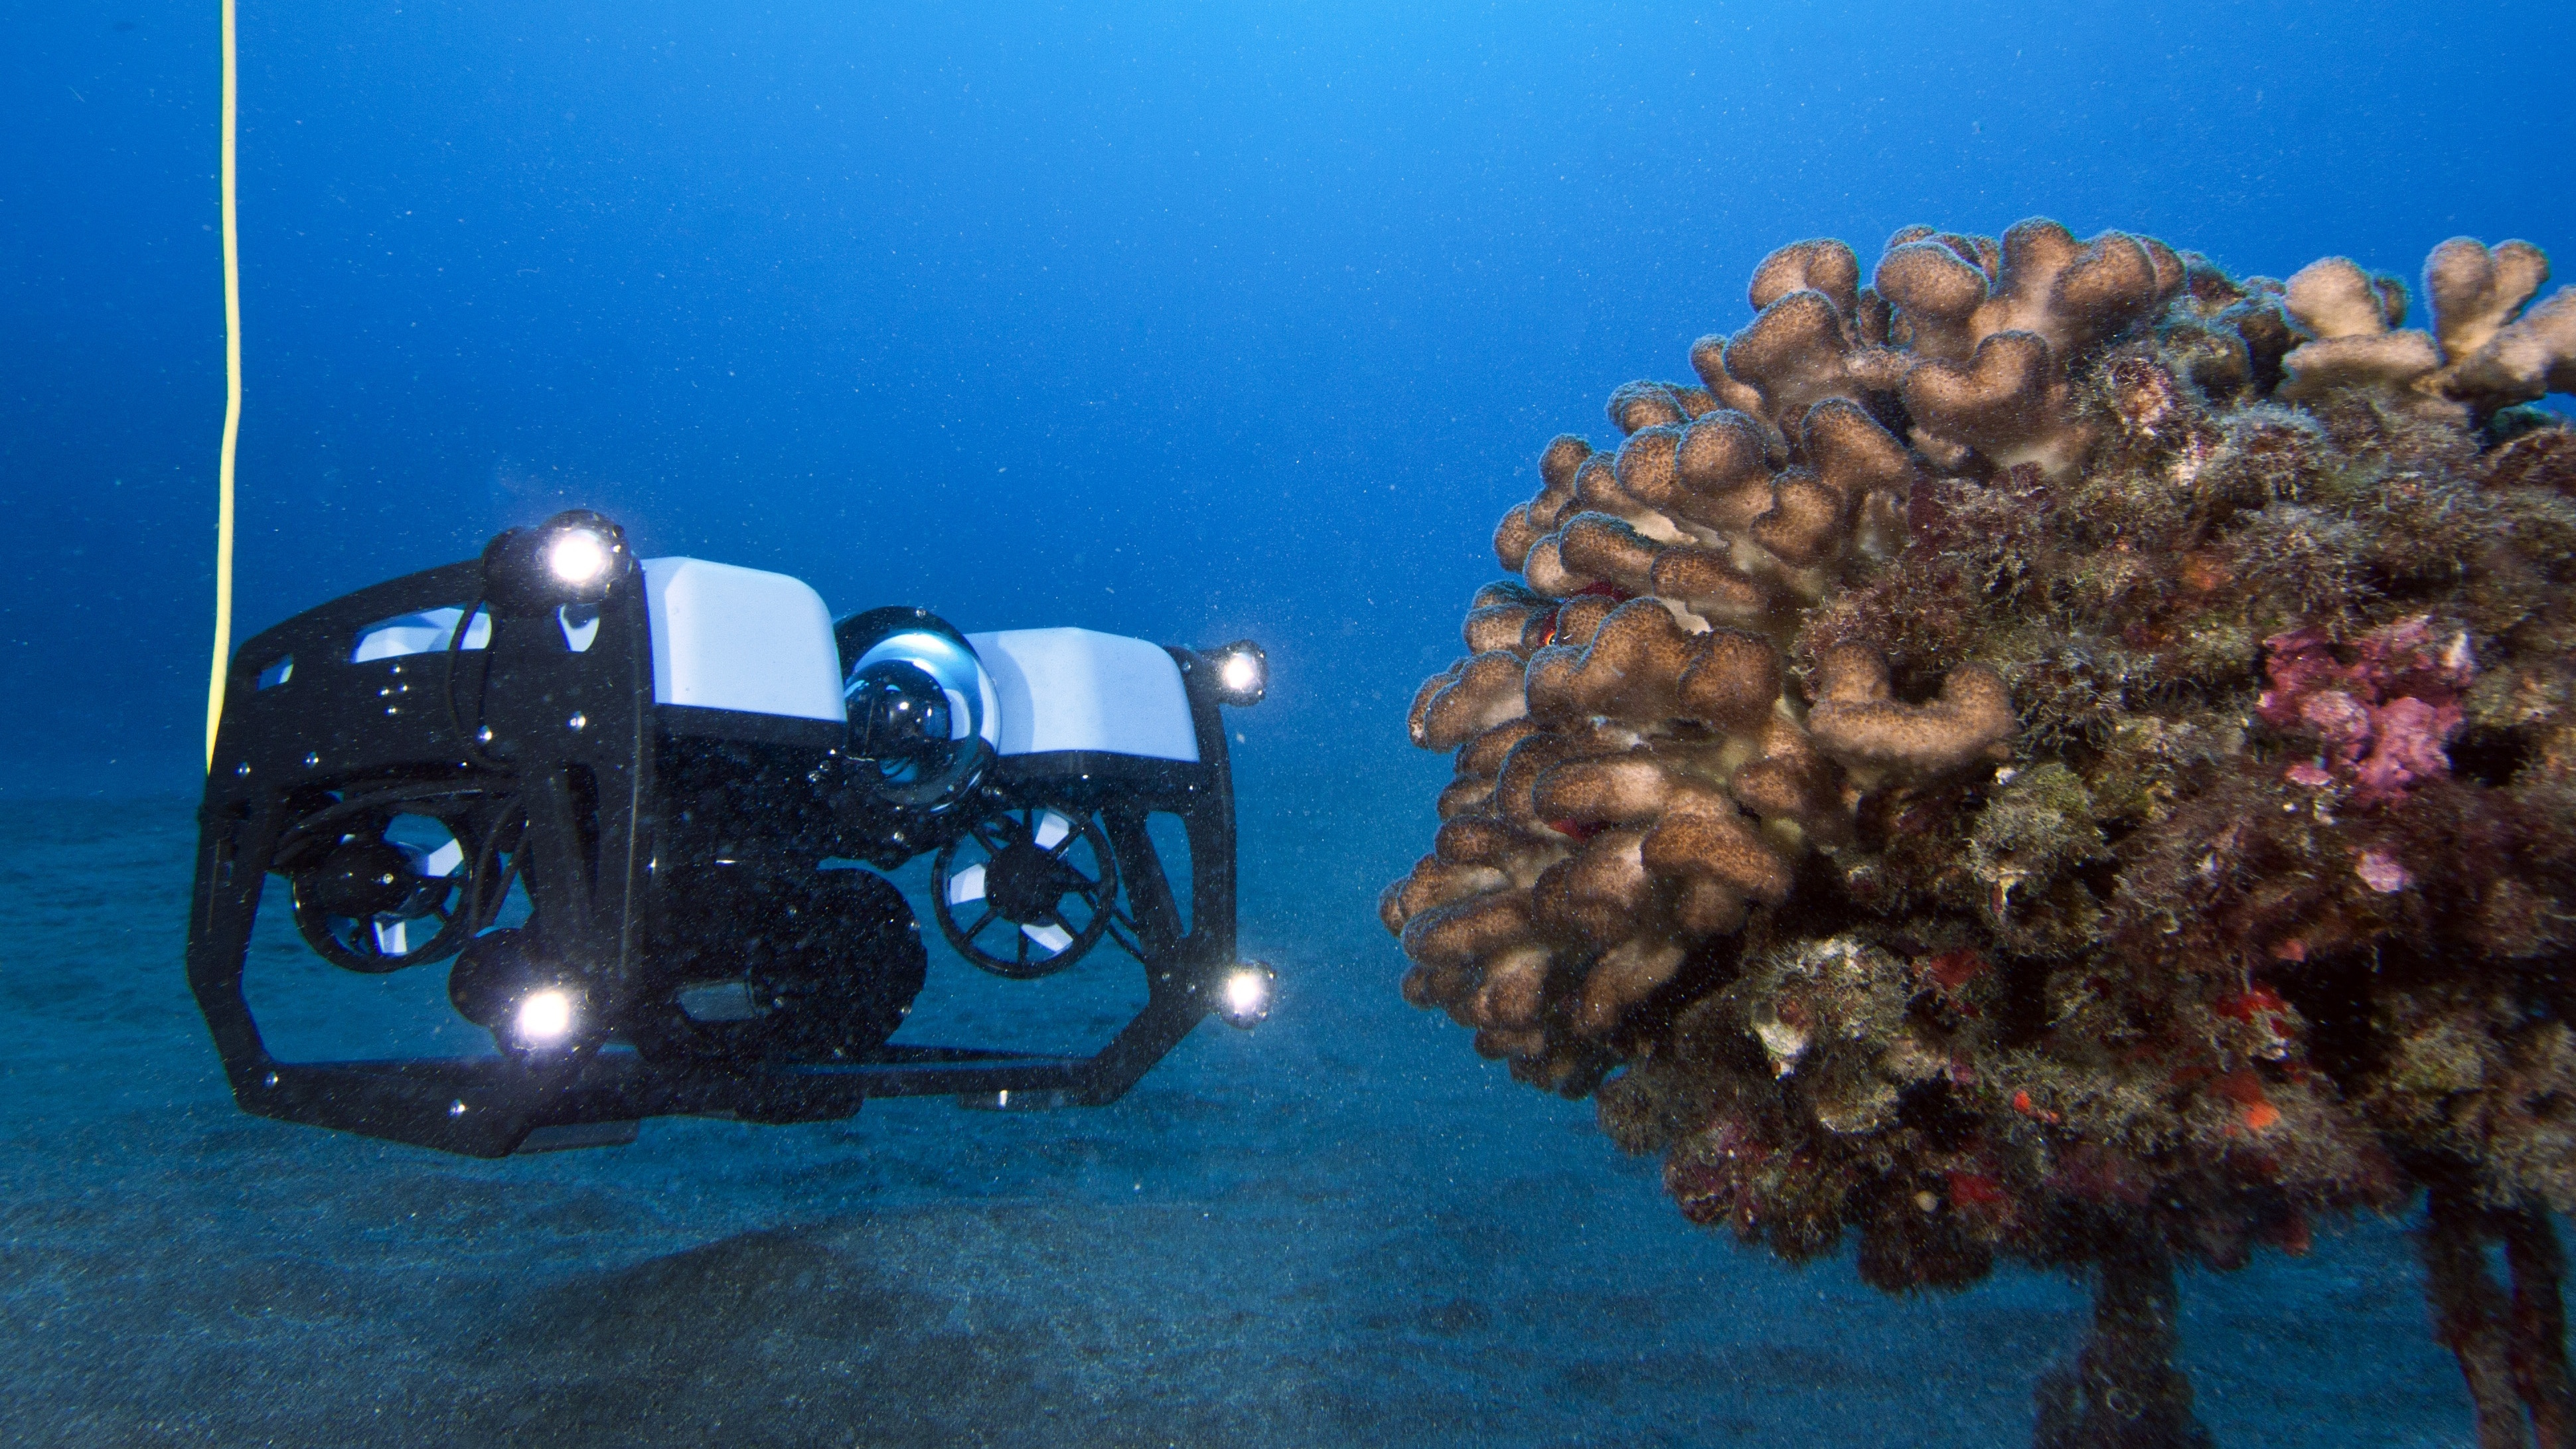
\includegraphics[width=\textwidth]{Phd_thesis/chapters/1.Introduction/figures/BlueROV2.jpg}
        \caption{BlueROV2 medium-sized tethered ROV \cite{bluerobotics_bluerov2_nodate}.}
        \label{fig:subfig2}
    \end{subfigure}
    
    \vspace{0.5cm} % Adjust vertical space between rows
    
    % Second Row
    \begin{subfigure}[b]{0.46\textwidth}
        \centering
        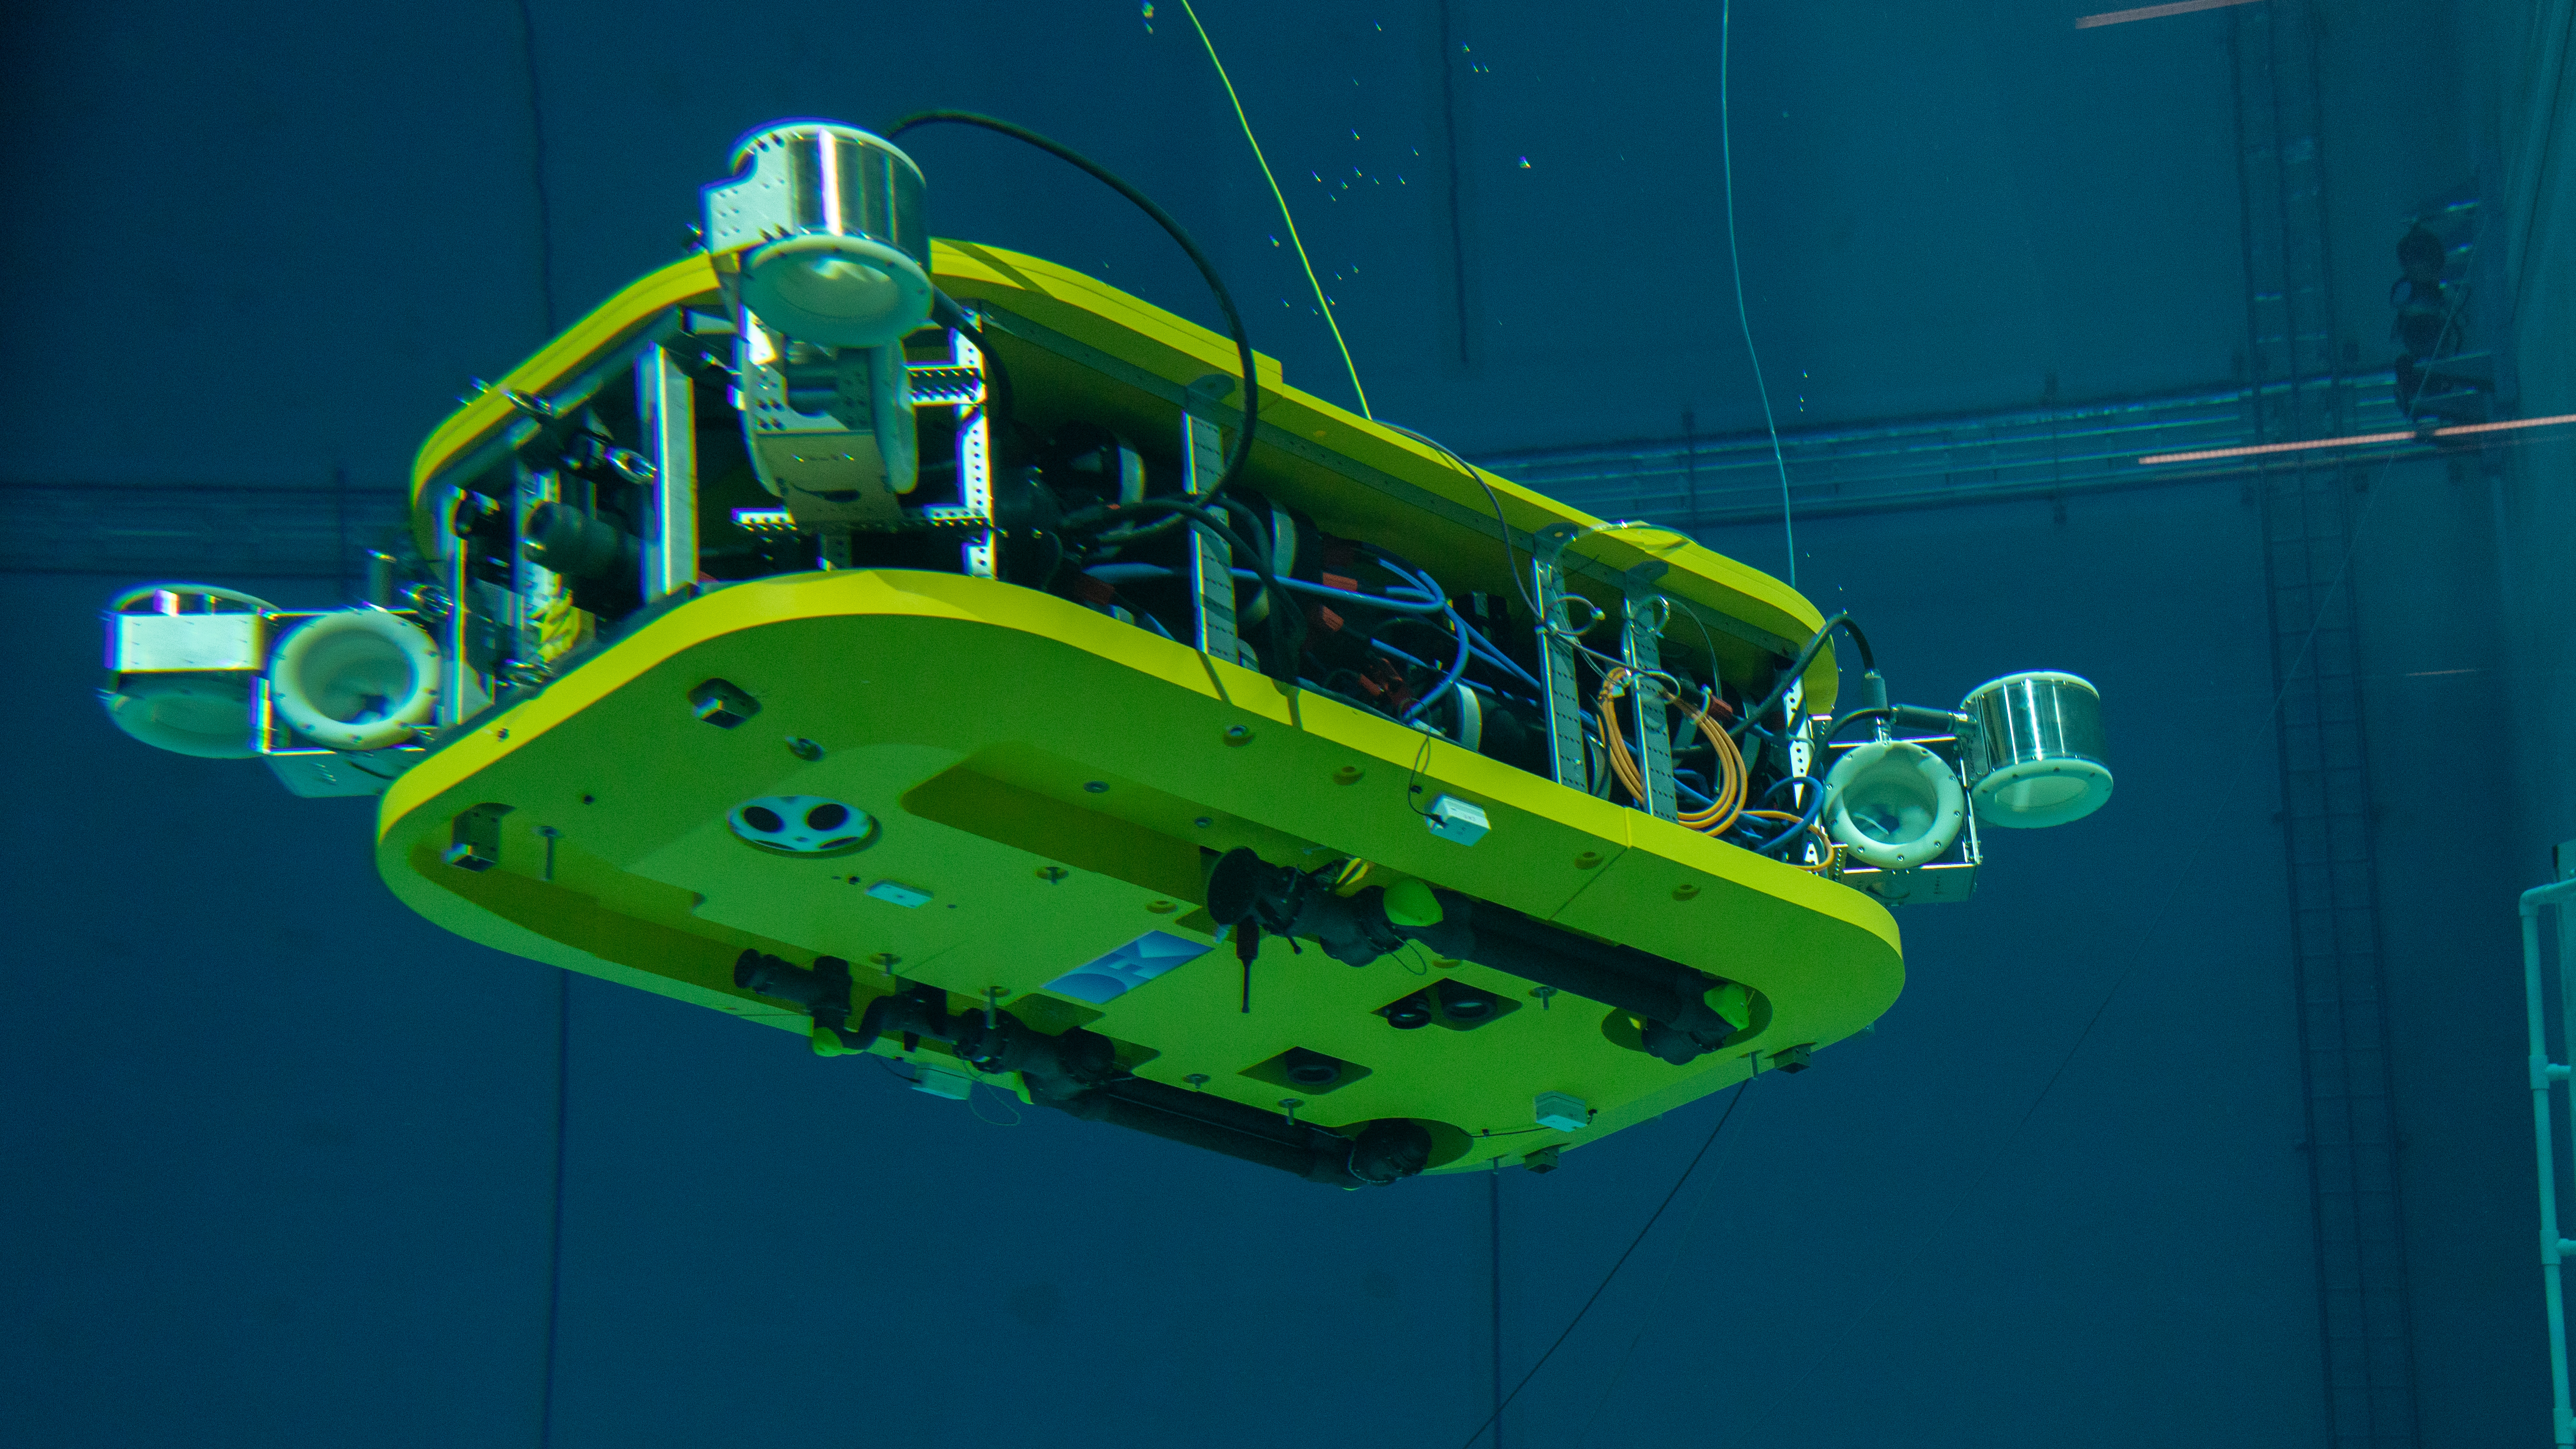
\includegraphics[width=\textwidth]{Phd_thesis/chapters/1.Introduction/figures/cuttlefish.jpg}
        \caption{DFKI Cuttlefish autonomous underwater vehicle \cite{christensen_cuttlefish_nodate}.}
        \label{fig:subfig3}
    \end{subfigure}
    \hfill
    \begin{subfigure}[b]{0.49\textwidth}
        \centering
        \includegraphics[width=\textwidth]{Phd_thesis/chapters/1.Introduction/figures/scanfish_towed.jpg}
        \caption{EIVA ScanFish Rocio remotely operated towed vehicle \cite{eiva_scanfish_nodate}.}
        \label{fig:subfig4}
    \end{subfigure}
    
    \caption{Showcase of the variety Marine Robotics Platforms.}
    \label{fig:underwater_robotics_applications}
\end{figure*}


Currently, many marine robotic tasks depend on remote control (teleoperation) or semi-autonomous functions, such as executing pre-programmed paths or simple line-following maneuvers. While effective for specific, well-defined tasks, these modes often necessitate skilled human pilots and constant supervision, limiting mission duration, complexity, and operational range.

The drive towards fully autonomous marine systems stems from the need to enhance operational safety, increase mission efficiency and capability, and reduce operational costs. By minimizing direct human intervention, autonomy mitigates the risk of human error, enables longer and more complex missions in challenging environments, and ultimately lowers operational expenses.


% --- Challenges to Autonomy ---
Achieving reliable underwater autonomy, however, requires overcoming fundamental challenges inherent to the complex and dynamic marine environment. Key among these are:

\begin{itemize}
    \item \textbf{Safe Navigation:} Ensuring safe navigation is essential, including robust obstacle avoidance and adherence to physical constraints. Many marine robots are tethered, so preventing tether entanglement during operation is a critical safety consideration.

    \item \textbf{Precise and Robust Trajectory Following:} The ability to accurately follow desired trajectories under disturbances such as ocean currents is fundamental for mission success in complex marine environments.

    \item \textbf{Generalizability Across Different Platforms:} Control and planning methods should transfer across a wide range of robotic platforms—such as UAVs, AUVs, and systems with varying sizes and degrees of freedom—without the need for substantial redesign or tuning.
\end{itemize}



















 %\subsection{Optimal Control in Marine Autonomy}

%Why optimal control is needed
Trajectory optimization has become central to recent breakthroughs in autonomy, enabling robots to perform increasingly complex tasks. By formulating trajectory planning as an optimization problem—where high-level objectives are specified rather than relying on predefined sequences of actions—systems can adapt and respond intelligently to dynamic environments. At the heart of this trajectory optimization lies Model Predictive Control (MPC) which allows simultaneous optimization of trajectories and control inputs in real time. It naturally accommodates the coupled dynamics and high degrees of freedom characteristic of autonomous vehicles, while explicitly handling constraints related to thruster limitations, operational boundaries, and collision avoidance. This integration of real-time planning, dynamic feasibility, and constraint satisfaction has unlocked new capabilities in marine autonomy that were previously out of reach using conventional methods.




    

    
    

    
 \subsection{Critical Barriers to \ac{MPC} Adoption in Marine Robotics Inspection Tasks}
\label{subsec:mpc_barriers}

While \ac{MPC} improves autonomous capabilities, there are fundamental challenges that could hinder \ac{MPC}'s performance and deployment in marine environments, which include:

\textbf{1. Simulation-Reality Discrepancy:} Existing underwater simulators lack both \textit{visual realism} (critical for perception algorithms) and \textit{physical fidelity} in modeling hydrodynamic interactions, making pre-deployment controller validation unreliable. This gap forces costly trial-and-error field testing.

\textbf{2. Environmental Uncertainty:} Marine disturbances—waves, currents, —exhibit multi-scale spatiotemporal variations that defy analytical modeling. Traditional \ac{MPC} performance degrades rapidly when hydrodynamic predictions from reality.

\textbf{3. Mission-Safety Tradeoffs:} Simultaneously optimizing inspection coverage while preventing tether entanglement requires solving high-dimensional constraints in real time—a computationally intractable problem for conventional planners.

\textbf{4. Perception-Control Decoupling:} Current frameworks treat trajectory tracking and visual inspection as separate objectives, often sacrificing coverage quality for path accuracy or vice versa. This disconnect leads to incomplete data collection in turbid or cluttered environments.

These challenges form a self-reinforcing cycle: poor simulation prevents controller refinement, environmental uncertainty degrades predictions, and safety constraints limit mission complexity. Overcoming this requires co-designing robust simulation tools, adaptive modeling techniques, and task-aware control architectures—the focus of this work.
 
% Define colors (ensure these are defined in your main document preamble)
\definecolor{navyblue}{rgb}{0.0, 0.0, 0.5}
\definecolor{cyan}{rgb}{0.0, 1.0, 1.0}


\section{Hypothesis and Research Goals}
Building on the challenges identified in applying \ac{MPC} to marine robotic inspection tasks, the core hypothesis of this thesis is formulated as follows:


%\subsection{Core Hypothesis}
\begin{figure}[h!]
    \centering
    \begin{tikzpicture}[
        hypothesisbox/.style = {
            draw=navyblue,
            line width=1.5pt,
            rounded corners=8pt,
            fill=cyan!3,      % Light cyan fill
            inner sep=12pt,
            text width=0.9\textwidth,
            align=justify
        }
    ]
\node[hypothesisbox] {
Enhanced with \textbf{data-driven modeling}, \textbf{perception-aware trajectory optimization}, and \textbf{tether-aware planning frameworks}, \ac{MPC} enables autonomous marine robots to achieve improved trajectory tracking and inspection coverage while mitigating entanglement risks—outperforming conventional geometric planning and standard \ac{MPC} approaches.
};
    \end{tikzpicture}
    
    \label{fig:revised_hypothesis_separate}
\end{figure}

%what is this hypotehsis about and why did you make it?
This hypothesis proposes that three synergistic advancements to \ac{MPC} will fundamentally improve underwater inspection systems. The proposed enhancements specifically target persistent challenges in marine robotics through:

\begin{itemize}
    \item \textbf{Entanglement-Aware Planning:} Incorporating entanglement-aware constraints into the planning process to enhance mission safety and operational reliability.
    
      \item \textbf{Perception-Aware Control:} Embedding visual inspection objectives directly into the trajectory optimization process to maximize coverage quality and ensure robustness to environmental disturbances.
    
    \item \textbf{Data-Driven Modeling:} Leveraging learning-based approaches to capture complex and uncertain hydrodynamic effects that degrade the performance of conventional \ac{MPC} in real-world conditions.
    

\end{itemize}

\subsection{Research Goals}
The hypothesis is  be validated through development and testing of its constituent components:



\begin{enumerate}
\item \textbf{Design Adaptive Disturbance Learning Frameworks:}  
Develop a learning-based framework for estimating external disturbances and environmental perturbations, enabling robust performance of MPC.


\item \textbf{Formulate a Perception-Aware \ac{MPC} Framework:}  
Integrate visual inspection quality metrics directly into MPC cost functions

\item \textbf{Design Entanglement-Aware Coverage Framework:}  
Develop real-time path planning with explicit entanglement prevention constraints

\item \textbf{Develop a Visually-Realistic Marine Robotics Simulation Platform:}  
Establish a synthetic testing environment bridging simulation-to-reality gaps
\end{enumerate}



 \subsection{Evaluation Criteria}
The evaluation framework directly aligns with the research goals through quantitative metrics assessing each component's contribution to the core hypothesis.}

\begin{table}[h!]
\centering
\caption{Performance Metrics for Hypothesis Validation}
\label{tab:eval_metrics}
\footnotesize
\begin{tabular}{p{0.22\textwidth}p{0.73\textwidth}}
\toprule
\textbf{Component} & \textbf{Evaluation Metrics} \\
\midrule

\textbf{Tether-Aware Planning} &
\begin{itemize}[leftmargin=*,noitemsep]
\item \textit{Safety}: Max allowable tether length exceedance time
\item \textit{Coverage}: Completeness (\% inspected area) on complex structures
\item \textit{Computation time}
\end{itemize} \\

\textbf{Perception-Aware Control} &
\begin{itemize}[leftmargin=*,noitemsep]
\item \textit{Safety}: Distance from inspection surface
\item \textit{Inspection Quality}: How centered the surfaces being inspected (defined in paper). 
\item \textit{Robustness}: Performance under operational disturbances
\end{itemize} \\

\textbf{Data-Driven Modelling} &
\begin{itemize}[leftmargin=*,noitemsep]
\item  \textit{Modelling Error}: Mean squared error in predicting environmental disturbances
\item \textit{Trajectory Tracking Error}:  Mean squared error in trajectory tracking
\end{itemize} \\



\bottomrule
\end{tabular}
\end{table}

 \section{Thesis Structure and Contributions}

\begin{figure}[h!]
    \centering
    \includegraphics[width=1.0\textwidth]{Phd_thesis/chapters/1.Introduction/figures/contributions_thesis.pdf}
    \caption{Research contributions and their interdependencies in marine robotics autonomy}
    \label{fig:contribution_structure}
\end{figure}

The main scientific and technological contributions presented in this thesis are:

\begin{description}[leftmargin=1cm, style=unboxed, font=\normalfont] % Using description list for clarity

    \item[\textcolor{blue}{\textbf{[C1] Simulation Infrastructure}}] \hfill \\
        Provides the foundational platform for development and validation.
        \begin{itemize}[leftmargin=0.5cm, itemsep=0pt]
            \item \textbf{C1.1: Visually Realistic Underwater Robot Simulator:} Development of a simulation environment combining realistic visual rendering with accurate hydrodynamic modeling to reduce the sim-to-real gap.
        \end{itemize}

    \item[\textcolor{blue}{\textbf{[C2] Control and Planning}}] \hfill \\
        Develops novel algorithms for safe and effective autonomous navigation and task execution.
        \begin{itemize}[leftmargin=0.5cm, itemsep=0pt]
            \item \textbf{C2.1: Tether-Aware Path Planning:} Algorithms for generating collision-free and entanglement-aware trajectories for tethered underwater robots during complex inspection tasks.
            \item \textbf{C2.2: Perception-Aware NMPC Formulation:} An \ac{NMPC} strategy that explicitly incorporates visual tracking objectives and constraints, optimizing for both path following and inspection quality.
        \end{itemize}

    \item[\textcolor{blue}{\textbf{[C3] Model Learning}}] \hfill \\
        Enhances controller performance by improving the fidelity of the underlying dynamic models.
         \begin{itemize}[leftmargin=0.5cm, itemsep=0pt]
            \item \textbf{C3.1: Learning Full Model Dynamics using PINNs:} Exploration of Physics-Informed Neural Networks for learning comprehensive dynamic models from data while respecting physical laws.
            \item \textbf{C3.2: Learning Model Residuals using GP:} Online estimation of model uncertainties and external disturbances using \acp{GP} to adaptively augment the nominal model used within the \ac{MPC}.
        \end{itemize}
\end{description}


 
%tikz stuff
\definecolor{xaxisred}{RGB}{220,20,60}    % Crimson for x-axis
\definecolor{yaxisgreen}{RGB}{50,205,50}  % Lime Green for y-axis
\definecolor{zaxisblue}{RGB}{0,0,255}     % Blue for z-axis
\definecolor{earthblue}{RGB}{0,51,102}    % Darker blue for earth frame
\definecolor{bodyred}{RGB}{178,34,34}     % Red for body frame
\definecolor{oceancolor}{RGB}{0,105,148}  % Ocean color
\definecolor{seafloor}{RGB}{139,115,85}   % Seafloor color
\definecolor{rovblue}{RGB}{30,144,255}    % ROV blue color
\definecolor{rovframe}{RGB}{50,50,50}     % ROV frame color

% Set up the view angles
\tdplotsetmaincoords{70}{120}



\chapter{Background on Data-Driven Model Predictive Control for Marine Robots}
\label{ch:background}

This chapter establishes the foundation for MPC design and implementation. We begin with first-principles modeling of marine robots using the 6-DOF framework, examine data-driven approaches to address modeling limitations, and conclude with MPC fundamentals including trajectory optimization and Sequential Quadratic Programming solution methods.

\section{Modelling Marine Robots}
\label{sec:modelling}
Accurate dynamic models are fundamental to MPC performance. This section develops the 6-DOF mathematical framework for underwater vehicles using first principles, then examines data-driven approaches to address modeling limitations.
This section introduces the common principles of modelling marine robotics, particularly underwater vehicles, using first principles. A motion model is crucial for developing simulators, designing model-based controllers such as MPC.

\subsection{Frames of Reference}
Underwater vehicle motion is typically described using two coordinate systems: an earth-fixed (inertial) reference frame and a body-fixed reference frame attached to the vehicle.

The global reference frame, denoted $\mathcal{F}_E$, is fixed relative to the Earth. For marine applications, the North-East-Down (NED) coordinate system is commonly used. Its origin is often set at a convenient location (e.g., deployment point), with axes defined as follows: the $x$-axis points toward true North, the $y$-axis points toward East, and the $z$-axis points downward, perpendicular to the Earth's surface.

The body-fixed reference frame, denoted $\mathcal{F}_B$, moves with the vehicle. Its origin is usually placed at the vehicle's center of gravity (see Fig.~\ref{fig:coordinate_frame_brov}). Following the Society of Naval Architects and Marine Engineers (SNAME) convention, the axes are defined such that the $x$-axis points forward along the longitudinal axis, the $y$-axis points starboard (right), and the $z$-axis points downward.

\begin{figure}[h!] % Changed [b!] to [h!] for better placement flexibility, adjust as needed
    \centering
    \includegraphics[width=0.5\textwidth]{Phd_thesis/chapters/1.Introduction/figures/brov4.pdf} % Ensure path is correct
    \caption{Coordinate frames of the BlueROV underwater vehicle: the body-fixed frame, $\mathcal{F}_B$, is attached to the vehicle’s center of gravity, and the earth-fixed frame, $\mathcal{F}_E$, is inertial. The thruster configuration is also shown: vertical thrusters in green, horizontal thrusters in blue.}
    \label{fig:coordinate_frame_brov}
\end{figure}

The vehicle's state involves position, orientation, linear velocities, and angular velocities. The position and orientation in the earth frame $\mathcal{F}_E$ are represented by the vector $\boldsymbol{\eta} = [x, y, z, \phi, \theta, \psi]^T$, where $\phi$, $\theta$, and $\psi$ are the Euler angles (roll, pitch, yaw). The linear and angular velocities in the body frame $\mathcal{F}_B$ are represented by the vector $\boldsymbol{\nu} = [u, v, w, p, q, r]^T$.

\subsection{Newton-Euler Equations of Motion}
The dynamics of an underwater vehicle, treated as a rigid body moving in a fluid, can be derived using the Newton-Euler equations. These must account for hydrodynamic effects like added mass and damping, as well as gravitational and buoyancy forces.

Fossen's vectorial formulation provides a standard framework:
\begin{align}
    \dot{\boldsymbol{\eta}} &= \mathbf{J}(\boldsymbol{\eta})\boldsymbol{\nu} \label{eq:kinematics} \\
    \mathbf{M}\dot{\boldsymbol{\nu}} + \mathbf{C}(\boldsymbol{\nu})\boldsymbol{\nu} + \mathbf{D}(\boldsymbol{\nu})\boldsymbol{\nu} + \mathbf{g}(\boldsymbol{\eta}) &= \mathbf{u} + \boldsymbol{\Delta} \label{eq:dynamics}
\end{align}

Equation \eqref{eq:kinematics} describes the kinematics, relating the body-fixed velocity vector $\boldsymbol{\nu} = [u, v, w, p, q, r]^T$, where $[u, v, w]$ are linear velocities and $[p, q, r]$ are angular velocities, to the rate of change of position and orientation in the global frame $\dot{\boldsymbol{\eta}} = [\dot{x}, \dot{y}, \dot{z}, \dot{\phi}, \dot{\theta}, \dot{\psi}]^T$ through the transformation matrix $\mathbf{J}(\boldsymbol{\eta})$. The pose vector $\boldsymbol{\eta} = [x, y, z, \phi, \theta, \psi]^T$ consists of position coordinates $[x, y, z]$ and Euler angles (roll $\phi$, pitch $\theta$, yaw $\psi$). The vector $\mathbf{u} = [X, Y, Z, K, M, N]^T$ represents the control forces and moments generated by actuators (thrusters, fins, etc.). The vector $\boldsymbol{\Delta}$ represents external environmental disturbances (currents, waves).

The transformation matrix $\mathbf{J}(\boldsymbol{\eta})$ is defined as
\begin{equation}
    \mathbf{J}(\boldsymbol{\eta}) =
    \begin{bmatrix}
        \mathbf{R}(\phi,\theta,\psi) & \mathbf{0}_{3\times3} \\
        \mathbf{0}_{3\times3} & \mathbf{T}(\phi,\theta)
    \end{bmatrix}
\end{equation}
where $\mathbf{R}(\phi,\theta,\psi)$ is the rotation matrix from the body-fixed frame $\mathcal{F}_B$ to the global frame $\mathcal{F}_G$ using the ZYX Euler angle convention:
\begin{equation}
    \mathbf{R}(\phi,\theta,\psi) = \mathbf{R}_z(\psi)\mathbf{R}_y(\theta)\mathbf{R}_x(\phi)
\end{equation}
and $\mathbf{T}(\phi,\theta)$ is the transformation matrix that maps body angular velocities to Euler angle rates:
\begin{equation}
    \mathbf{T}(\phi,\theta) =
    \begin{bmatrix}
        1 & \sin\phi \tan\theta & \cos\phi \tan\theta \\
        0 & \cos\phi & -\sin\phi \\
        0 & \sin\phi / \cos\theta & \cos\phi / \cos\theta
    \end{bmatrix}
\end{equation}
%Note that $\mathbf{T}(\phi,\theta)$ becomes singular when the pitch angle $\theta$ approaches $\pm 90^\circ$.

Equation \eqref{eq:dynamics} represents the dynamics of the vehicle. The system inertia matrix $\mathbf{M}$ is composed of the rigid-body inertia matrix $\mathbf{M}_{RB}$ and the hydrodynamic added mass matrix $\mathbf{M}_A$:
\begin{equation}
    \mathbf{M} = \mathbf{M}_{RB} + \mathbf{M}_A.
\end{equation}
The rigid-body inertia matrix $\mathbf{M}_{RB}$ is expressed as
\begin{equation}
    \mathbf{M}_{RB} =
    \begin{bmatrix}
        m \mathbf{I}_{3\times3} & -m \mathbf{S}(\boldsymbol{r}_G) \\
        m \mathbf{S}(\boldsymbol{r}_G) & \mathbf{I}_G
    \end{bmatrix}
\end{equation}
where $m$ is the vehicle mass, $\mathbf{I}_{3\times3}$ is the $3 \times 3$ identity matrix, $\boldsymbol{r}_G = [x_G, y_G, z_G]^T$ is the position vector of the center of gravity (CG) relative to the body-fixed frame, and $\mathbf{I}_G$ is the inertia tensor about the CG. The matrix $\mathbf{S}(\boldsymbol{r}_G)$ is the skew-symmetric matrix associated with $\boldsymbol{r}_G$, given by
\begin{equation}
    \mathbf{S}(\boldsymbol{r}_G) =
    \begin{bmatrix}
        0 & -z_G & y_G \\
        z_G & 0 & -x_G \\
        -y_G & x_G & 0
    \end{bmatrix}.
\end{equation}


The Coriolis-centripetal matrix $\mathbf{C}(\boldsymbol{\nu})$ represents the Coriolis and centripetal forces arising from vehicle motion, while the damping matrix $\mathbf{D}(\boldsymbol{\nu})$ models hydrodynamic drag forces. The restoring forces and moments due to gravity and buoyancy are encapsulated in the vector $\mathbf{g}(\boldsymbol{\eta})$. 
 
The added mass matrix $\mathbf{M}_A$ accounts for the inertia contribution of the fluid accelerated by the vehicle motion. It is typically represented using hydrodynamic derivatives:
\begin{equation}
    \mathbf{M}_{A} = -
    \begin{bmatrix}
        X_{\dot{u}} & X_{\dot{v}} & X_{\dot{w}} & X_{\dot{p}} & X_{\dot{q}} & X_{\dot{r}} \\
        Y_{\dot{u}} & Y_{\dot{v}} & Y_{\dot{w}} & Y_{\dot{p}} & Y_{\dot{q}} & Y_{\dot{r}} \\
        Z_{\dot{u}} & Z_{\dot{v}} & Z_{\dot{w}} & Z_{\dot{p}} & Z_{\dot{q}} & Z_{\dot{r}} \\
        K_{\dot{u}} & K_{\dot{v}} & K_{\dot{w}} & K_{\dot{p}} & K_{\dot{q}} & K_{\dot{r}} \\
        M_{\dot{u}} & M_{\dot{v}} & M_{\dot{w}} & M_{\dot{p}} & M_{\dot{q}} & M_{\dot{r}} \\
        N_{\dot{u}} & N_{\dot{v}} & N_{\dot{w}} & N_{\dot{p}} & N_{\dot{q}} & N_{\dot{r}}
    \end{bmatrix}
\end{equation}
where $X_{\dot{u}}$ is the added mass force in $x$-direction due to surge acceleration $\dot{u}$, etc.

The matrix $\mathbf{C}(\boldsymbol{\nu})$ represents Coriolis and centripetal forces, including rigid-body $\mathbf{C}_{RB}(\boldsymbol{\nu})$ and added mass $\mathbf{C}_A(\boldsymbol{\nu})$ terms:
\begin{equation}
    \mathbf{C}(\boldsymbol{\nu}) = \mathbf{C}_{RB}(\boldsymbol{\nu}) + \mathbf{C}_A(\boldsymbol{\nu})
\end{equation}
These terms arise from the rotation of the body frame and the interaction of the vehicle with the fluid.

The damping matrix $\mathbf{D}(\boldsymbol{\nu})$ represents hydrodynamic drag forces and moments opposing motion. It is often decomposed into linear $\mathbf{D}_{lin}$ and nonlinear (quadratic) $\mathbf{D}_{nonlin}(\boldsymbol{\nu})$ components:
\begin{equation}
    \mathbf{D}(\boldsymbol{\nu}) = \mathbf{D}_{lin} + \mathbf{D}_{nonlin}(\boldsymbol{\nu})
\end{equation}
Linear damping is often approximated as diagonal:
\begin{equation}
    \mathbf{D}_{lin} = -\text{diag}(X_u, Y_v, Z_w, K_p, M_q, N_r)
\end{equation}
Nonlinear damping, modeled as a quadratic function of the velocity, is expressed as:



\begin{equation}
    \mathbf{D}_{nonlin}(\boldsymbol{\nu}) = -\text{diag}(X_{u|u|}|u|, Y_{v|v|}|v|, Z_{w|w|}|w|, K_{p|p|}|p|, M_{q|q|}|q|, N_{r|r|}|r|)
\end{equation}

The vector $\mathbf{g}(\boldsymbol{\eta})$ represents restoring forces and moments due to gravity (weight $W=mg$) and buoyancy ($B$). If the CG and center of buoyancy (CB) at $\boldsymbol{r}_B = [x_B, y_B, z_B]^T$ do not coincide, these forces create moments:
\begin{equation}
    \mathbf{g}(\boldsymbol{\eta}) =
    \begin{bmatrix}
        (W-B)\sin\theta \\
        -(W-B)\cos\theta\sin\phi \\
        -(W-B)\cos\theta\cos\phi \\
        (y_G W - y_B B)\cos\theta\cos\phi - (z_G W - z_B B)\cos\theta\sin\phi \\
        -(x_G W - x_B B)\cos\theta\cos\phi - (z_G W - z_B B)\sin\theta \\ % Corrected signs based on Fossen convention
        -(x_G W - x_B B)\cos\theta\sin\phi + (y_G W - y_B B)\sin\theta % Corrected signs based on Fossen convention
    \end{bmatrix}
\end{equation}



Combining the kinematic and dynamic equations \eqref{eq:kinematics} and \eqref{eq:dynamics}, the nonlinear state-space model of the underwater vehicle can be expressed compactly as
\begin{equation}
    \dot{\boldsymbol{x}} = f(\boldsymbol{x}, \mathbf{u}) = 
    \begin{bmatrix}
        \dot{\boldsymbol{\eta}} \\
        \dot{\boldsymbol{\nu}}
    \end{bmatrix}
    =
    \begin{bmatrix}
        \mathbf{J}(\boldsymbol{\eta}) \boldsymbol{\nu} \\
        \mathbf{M}^{-1} \big( \mathbf{u} + \boldsymbol{\Delta} - \mathbf{C}(\boldsymbol{\nu}) \boldsymbol{\nu} - \mathbf{D}(\boldsymbol{\nu}) \boldsymbol{\nu} - \mathbf{g}(\boldsymbol{\eta}) \big)
    \end{bmatrix}.
\end{equation}
Here, the state vector is defined as \(\boldsymbol{x} = [\boldsymbol{\eta}^T, \boldsymbol{\nu}^T]^T\).



The control wrench \(\mathbf{u}\) is generated by the individual thruster outputs. For a vehicle equipped with \(n\) thrusters, where the \(i\)-th thruster produces thrust \(T_i\), the total wrench is modeled as
\begin{equation}
    \mathbf{u} = \mathbf{B} \boldsymbol{T},
\end{equation}
where \(\boldsymbol{T} = [T_1, T_2, \ldots, T_n]^T\) is the vector of thruster commands, and \(\mathbf{B}\) is the \(6 \times n\) thrust allocation matrix. Each column \(\mathbf{B}_i\) maps the thrust \(T_i\) to forces and moments in the body frame \(\mathcal{F}_B\), based on the thruster’s position \(\boldsymbol{r}_i\) and unit thrust direction vector \(\boldsymbol{d}_i\):
\begin{equation}
    \mathbf{B}_i = \begin{bmatrix} \boldsymbol{d}_i \\ \boldsymbol{r}_i \times \boldsymbol{d}_i \end{bmatrix}.
\end{equation}

%%%%%%%%%%%%%%%%
%%%%%%%%%%%%%%%
% DATA-DRIVEN 
%%%%%%%%%%%%%%%
%%%%%%%%%%%%%%%

\subsection{Data-Driven Modeling of Underwater Vehicle Dynamics}
%\subsection{Model Limitations and model learning}
Given these inherent modeling limitations, there is a growing interest in leveraging data-driven techniques to enhance the fidelity of underwater vehicle dynamics. While physics-based models like Fossen’s provide a solid foundation, they often fail to capture complex or unmodeled phenomena such as unsteady hydrodynamics, fluid-structure interactions, or environmental disturbances with sufficient accuracy. To address these gaps, learning-based approaches have emerged as powerful tools that can either replace or augment traditional models. These methods generally fall into two main categories: \textit{full model learning}, where the entire system dynamics are inferred directly from data, and \textit{residual dynamics learning}, where a correction term is learned to compensate for inaccuracies in an existing physics-based model. Both strategies offer complementary pathways for improving model accuracy and generalization in real-world, uncertain, and dynamic underwater environments.



\subsubsection{Full Parametric Model Learning}

In the full parametric model learning approach, the entire dynamic behavior of the vehicle is learned directly from data. This method assumes that the governing dynamics are either unknown or too complex to model accurately from first principles. The objective is to identify a parameterized function $\hat{f}(\boldsymbol{x}, \mathbf{u}; \boldsymbol{\theta})$ that approximates the true system dynamics:

\begin{equation}
    \dot{\boldsymbol{x}} = \hat{f}(\boldsymbol{x}, \mathbf{u}; \boldsymbol{\theta})
\end{equation}

Here, $\boldsymbol{\theta}$ represents the vector of model parameters that are learned from data. The learning process begins by collecting a dataset of time-series measurements, where the corresponding time derivatives $\dot{\boldsymbol{x}}_i$ are typically estimated using numerical differentiation. This results in a dataset of input-output pairs:
\[
\mathcal{D} = \left\{ \big((\boldsymbol{x}_i, \mathbf{u}_i),\ \dot{\boldsymbol{x}}_i \big) \right\}_{i=1}^N,
\]



The goal is to find the optimal parameters $\boldsymbol{\theta}^*$ that minimize the discrepancy between the model's predictions and the observed data. This can be formulated as a least-squares regression problem:

\begin{equation}
    \boldsymbol{\theta}^* = \arg \min_{\boldsymbol{\theta}} \sum_{i=1}^N \left\| \dot{\boldsymbol{x}}_i - \hat{f}(\boldsymbol{x}_i, \mathbf{u}_i; \boldsymbol{\theta}) \right\|^2
\end{equation}

Various function approximators can be used for $\hat{f}$~\cite{brunton2025machine}. Neural networks offer great flexibility in capturing complex nonlinearities but often require large datasets and lack interpretability. For more interpretable models, the Sparse Identification of Nonlinear Dynamics (SINDy) method identifies a sparse set of governing equations from a library of candidate functions. Another approach is Gaussian process regression, a non-parametric method that provides uncertainty quantification. Its hyperparameters are typically optimized by maximizing the marginal log-likelihood~\cite{rasmussen_gaussian_2008}.

\subsubsection{Residual Dynamics Learning}
While full model learning captures the entire system behavior from data, an alternative is to retain the nominal physics-based model and learn only the discrepancy. This leads to the residual dynamics learning approach. To train the correction model, the same time-series dataset used for full model learning—comprising state, velocity, acceleration, and control inputs—is utilized. Rather than learning the complete dynamics, the residual approach leverages the nominal model to estimate the predicted acceleration and isolates the discrepancy as a residual term. This residual force and moment vector is computed by rearranging the nominal dynamics equation~\eqref{eq:dynamics}:

\begin{equation}
    \boldsymbol{\Delta }= \mathbf{M} \dot{\boldsymbol{\nu}} + \mathbf{C}(\boldsymbol{\nu}) \boldsymbol{\nu} + \mathbf{D}(\boldsymbol{\nu}) \boldsymbol{\nu} + \mathbf{g}(\boldsymbol{\eta}) - \mathbf{u}.
\end{equation}

The resulting residual $\boldsymbol{\Delta}$ is used as the training target for a model that maps the measured state and input pair $(\boldsymbol{x}, \mathbf{u})$ to the residual $\hat{\boldsymbol{\Delta}}$, thereby capturing unmodeled dynamics such as unsteady hydrodynamic effects, actuator nonlinearities, or external disturbances.



The choice between full model learning and residual learning depends on the fidelity of the existing model, availability of domain knowledge, and the nature and volume of data. Full model learning provides maximum flexibility and is well-suited to data-rich scenarios with poorly understood dynamics. Residual learning, in contrast, leverages existing knowledge to guide the learning process and generally requires less data to achieve comparable accuracy. Both approaches can be integrated with MPC, enabling robust and high-performance operation in uncertain and dynamic underwater environments.





 % Assuming Chapter/Section numbering continues from previous context
\section{Overview of Model Predictive Control}

Model Predictive Control (MPC) is an advanced control strategy that leverages a dynamic model of the system to predict its future behavior and optimize control actions over a finite time period, known as the prediction horizon ($T_p$). At each control cycle, MPC solves an online optimization problem to find a sequence of future control inputs that minimize a predefined cost function, subject to constraints on the system's states and inputs.

A key characteristic of MPC is its receding horizon approach. Although an entire sequence of future control inputs is computed, only the first input in the sequence is applied to the system over the next sampling interval ($\delta$). At the subsequent time step, the system's state is measured or estimated, and the prediction horizon shifts forward. The optimization problem is then solved again with this updated information, providing feedback and adapting to changing conditions.

For underwater vehicles, MPC offers significant benefits:
\begin{itemize}
    \item \textbf{Constraint Handling:} Systematically incorporates operational limits, such as maximum thruster forces (represented as limits on generalized forces $\boldsymbo{\tau}$), velocity restrictions, or safe operating areas, directly into the control problem formulation.
    \item \textbf{Predictive Capability:} Anticipates future system behavior, allowing proactive control actions in response to reference trajectory changes or predictable disturbances.
    \item \textbf{Optimality:} Balances competing objectives, such as precise trajectory tracking versus minimizing control effort, through the design of the cost function.
    \item \textbf{Nonlinearity Handling:} Can explicitly utilize the nonlinear dynamic models (as derived previously, e.g., in Section \ref{sec}), capturing complex hydrodynamic effects more accurately than linear controllers.
\end{itemize}


\subsection{The MPC Algorithm Formulation}
The core MPC algorithm involves repeatedly solving an optimal control problem. Let the system state be $\boldsymbol{x} = [\boldsymbol{\eta}^T, \boldsymbol{\nu}^T]^T \in \mathbb{R}^{12}$ (combining position/orientation and velocities), and the control input be the generalized force/moment vector $\boldsymbol{\tau} \in \mathbb{R}^6$. The continuous-time dynamics are $\dot{\boldsymbol{x}} = f(\boldsymbol{x}, \boldsymbol{\tau})$, representing the vehicle's equations of motion.

The optimization problem solved at time $t$ is typically formulated as:
\begin{mini!}|s|
{\substack{\boldsymbol{\bar{\tau}}(\cdot) \\ \text{over } [t, t+T_p]}}
{J = \int_t^{t+T_p} L(\boldsymbol{\bar{x}}(\sigma), \boldsymbol{\bar{\tau}}(\sigma)) \, d\sigma + E(\boldsymbol{\bar{x}}(t+T_p))}
{\label{eq:mpc_opt}}
{}
\addConstraint{\dot{\boldsymbol{\bar{x}}}(\sigma)}{= f(\boldsymbol{\bar{x}}(\sigma), \boldsymbol{\bar{\tau}}(\sigma))}{\quad \forall \sigma \in [t, t+T_p]}
\addConstraint{\boldsymbol{\bar{x}}(t)}{= \boldsymbol{x}(t)}{}
\addConstraint{\boldsymbol{\bar{\tau}}(\sigma)}{\in \mathbb{T}}{\quad \forall \sigma \in [t, t+T_p]}
\addConstraint{\boldsymbol{\bar{x}}(\sigma)}{\in \mathbb{X}}{\quad \forall \sigma \in [t, t+T_p]}
\end{mini!}

In this formulation, $\boldsymbol{\bar{x}}(\sigma)$ and $\boldsymbol{\bar{\tau}}(\sigma)$ represent the predicted state and control trajectories over the prediction horizon $[t, t+T_p]$, while $\boldsymbol{x}(t)$ denotes the current measured or estimated state. The stage cost $L(\cdot, \cdot)$ is typically defined as a quadratic function $L(\boldsymbol{x}, \boldsymbol{\tau}) = \|\boldsymbol{x} - \boldsymbol{x}_{ref}\|_{\boldsymbol{Q}}^2 + \|\boldsymbol{\tau}\|_{\boldsymbol{R}}^2$, penalizing deviations from a reference state $\boldsymbol{x}_{ref}$ and control effort, weighted by matrices $\boldsymbol{Q} \succeq 0$ and $\boldsymbol{R} \succ 0$. The terminal cost $E(\cdot)$ is often expressed as $E(\boldsymbol{x}) = \|\boldsymbol{x} - \boldsymbol{x}_{ref}(t+T_p)\|_{\boldsymbol{P}}^2$, with $\boldsymbol{P} \succeq 0$ selected based on stability considerations. The sets $\mathbb{T}$ and $\mathbb{X}$ define the admissible control inputs and states, respectively.

The MPC control loop is summarized in Algorithm \ref{alg:mpc_loop}.
\begin{algorithm}[H]
\caption{MPC Control Loop}
\label{alg:mpc_loop}
\begin{algorithmic}[1]
    \State At time $t$, measure or estimate the current state $\boldsymbol{x}(t)$.
    \State Solve the optimal control problem \eqref{eq:mpc_opt} to obtain the optimal control sequence $\boldsymbol{\bar{\tau}}^*(\sigma)$ for $\sigma \in [t, t+T_p]$.
    \State Apply only the first part of the optimal control input, $\boldsymbol{\tau}_{MPC}(t) = \boldsymbol{\bar{\tau}}^*(t)$, to the system (or as input to a lower-level control allocation if used) over the interval $[t, t+\delta)$.
    \State Wait until the next sampling time $t+\delta$. Set $t \leftarrow t+\delta$ and go back to Step 1.
\end{algorithmic}
\end{algorithm}





\subsection{Discretization for Numerical Solution}
The continuous-time optimal control problem \eqref{eq:mpc_opt} must be discretized to be solved numerically. The prediction horizon $T_p$ is divided into $N$ intervals of length $\Delta t = T_p/N$. A common approach is to assume piecewise constant control inputs over each interval:
\begin{equation}
    \boldsymbo{\tau}(t) = \boldsymbo{\tau}_k \quad \text{for} \quad t \in [t_k, t_{k+1}), \quad k = 0, \dots, N-1
\end{equation}
where $t_k = t + k\Delta t$. The continuous state dynamics $\dot{\boldsymbo{x}} = f(\boldsymbo{x}, \boldsymbo{\tau})$ are discretized using a numerical integration method (e.g., Euler, Runge-Kutta) to obtain a discrete-time prediction model:
\begin{equation}
    \boldsymbo{x}_{k+1} = f_d(\boldsymbo{x}_k, \boldsymbo{\tau}_k)
\end{equation}
For instance, using the 4th-order Runge-Kutta (RK4) method:
\begin{equation}
    \boldsymbo{x}_{k+1} = \boldsymbo{x}_k + \frac{\Delta t}{6}(\mat{k}_1 + 2\mat{k}_2 + 2\mat{k}_3 + \mat{k}_4)
\end{equation}
where $\mat{k}_1 = f(\boldsymbo{x}_k, \boldsymbo{\tau}_k)$, $\mat{k}_2 = f(\boldsymbo{x}_k + \frac{\Delta t}{2}\mat{k}_1, \boldsymbo{\tau}_k)$, etc.
The cost function integral is approximated by a sum:
\begin{equation}
    J_d = \sum_{k=0}^{N-1} L_d(\boldsymbo{x}_k, \boldsymbo{\tau}_k) + E(\boldsymbo{x}_N)
\end{equation}
where $L_d(\boldsymbo{x}_k, \boldsymbo{\tau}_k) \approx \int_{t_k}^{t_{k+1}} L(\boldsymbo{\bar{x}}(\sigma), \boldsymbo{\tau}_k) \, d\sigma$, often simplified to $L_d = \Delta t \left( \|\boldsymbo{x}_k - \boldsymbo{x}_{ref,k}\|_{\mat{Q}}^2 + \|\boldsymbo{\tau}_k\|_{\mat{R}}^2 \right)$.

\subsection{Solving the Optimization Problem}
Discretization transforms the optimal control problem into a Nonlinear Program (NLP). The decision variables are the sequence of control inputs $\boldsymbo{T}_U = \{\boldsymbo{\tau}_0, \dots, \boldsymbo{\tau}_{N-1}\}$.

\subsubsection{Direct Methods}
Direct methods treat both the control inputs $\boldsymbo{T}_U$ and the resulting state sequence $\boldsymbo{T}_X = \{\boldsymbo{x}_1, \dots, \boldsymbo{x}_N\}$ as optimization variables (with $\boldsymbo{x}_0 = \boldsymbo{x}(t)$ fixed). The discretized dynamics $ \boldsymbo{x}_{k+1} = f_d(\boldsymbo{x}_k, \boldsymbo{\tau}_k) $ are enforced as equality constraints. The NLP takes the form:
\begin{equation}
\begin{aligned}
\min_{\boldsymbo{T}_U, \boldsymbo{T}_X} \quad & \sum_{k=0}^{N-1} L_d(\boldsymbo{x}_k, \boldsymbo{\tau}_k) + E(\boldsymbo{x}_N) \\
\text{s.t.} \quad & \boldsymbo{x}_{k+1} = f_d(\boldsymbo{x}_k, \boldsymbo{\tau}_k), \quad k=0, \dots, N-1 \\
& \boldsymbo{\tau}_k \in \mathbb{T}, \quad k=0, \dots, N-1 \\
& \boldsymbo{x}_k \in \mathbb{X}, \quad k=1, \dots, N \\
& \boldsymbo{x}_0 = \boldsymbo{x}(t)
\end{aligned}
\end{equation}
This structured NLP can be solved using general-purpose NLP solvers.

\subsubsection{Sequential Quadratic Programming (SQP)}
SQP is a common iterative method for solving NLPs. At each iteration $k$, it approximates the NLP by a Quadratic Program (QP) obtained by linearizing the constraints and using a quadratic approximation of the Lagrangian function. The QP subproblem typically looks like:
\begin{equation}
\begin{aligned}
\min_{\Delta\boldsymbo{z}} \quad & \frac{1}{2}\Delta\boldsymbo{z}^T \mat{H}_k \Delta\boldsymbo{z} + \boldsymbo{g}_k^T \Delta\boldsymbo{z} \\
\text{s.t.} \quad & \mat{A}_{eq,k} \Delta\boldsymbo{z} = \boldsymbo{b}_{eq,k} \\
& \mat{A}_{ineq,k} \Delta\boldsymbo{z} \leq \boldsymbo{b}_{ineq,k}
\end{aligned}
\end{equation}
where $\Delta\boldsymbo{z}$ represents the step change in the optimization variables (e.g., $\boldsymbo{T}_U, \boldsymbo{T}_X$), $\mat{H}_k$ approximates the Hessian of the Lagrangian, $\boldsymbo{g}_k$ is the gradient of the objective function, and $\mat{A}_{eq,k}, \mat{A}_{ineq,k}$ are Jacobians of the constraints, all evaluated at the current iterate $\boldsymbo{z}_k$. Solving this QP yields a search direction $\Delta\boldsymbo{z}$, and the next iterate is found using a line search.

% \subsection{Implementation Considerations}
% Implementing MPC effectively involves several practical aspects:

% \subsubsection{Real-Time Computation} % Kept this subsubsection title
% Solving the optimization problem online at each sampling instant $\delta$ requires significant computational power, especially for fast systems or long horizons. Techniques to enable real-time MPC include:
% \begin{itemize}
%     \item \textbf{Efficient Solvers:} Using structure-exploiting optimization algorithms (e.g., interior-point methods, active-set methods tailored for MPC).
%     \item \textbf{Warm-Starting:} Initializing the solver at time $t+\delta$ with the shifted optimal solution from time $t$.
%     \item \textbf{Reducing Complexity:} Using techniques like move blocking (keeping control input constant over several steps) or shortening the prediction horizon $T_p$. A common rule of thumb suggests $T_p$ should cover the dominant dynamics, e.g., 5-10 times the vehicle's main time constant.
%     \item \textbf{Constraint Softening:} Relaxing constraints slightly using penalty terms if the problem becomes infeasible, ensuring the solver always returns a (possibly suboptimal) solution.
% \end{itemize}

% \subsubsection{Other Considerations} % Combined stability mention here
% Beyond computational performance, ensuring the stability of the closed-loop system is a crucial aspect of practical MPC design, particularly when dealing with nonlinear dynamics and constraints. While rigorous stability guarantees often involve specific choices of terminal costs and constraints, these theoretical aspects are complex and depend heavily on the system and controller tuning. For this overview, we acknowledge stability as an important factor to consider during implementation and validation, although detailed analysis methods are not covered here.

% --- Optional: Combine Implementation Considerations into one subsection ---
\subsection{Implementation Considerations}
Implementing MPC effectively on a marine robot involves addressing several practical aspects.

Firstly, \textbf{real-time computation} is critical. Solving the optimization problem online at each sampling instant $\delta$ demands significant computational resources. Common techniques to achieve real-time performance include: using efficient, structure-exploiting optimization solvers; warm-starting the solver at time $t+\delta$ with the shifted solution from time $t$; reducing problem complexity via methods like move blocking (keeping control inputs constant over several steps) or adjusting the prediction horizon $T_p$ (which typically needs to be long enough to capture relevant dynamics); and potentially using constraint softening to handle occasional infeasibility gracefully.

Secondly, while the receding horizon nature provides feedback, \textbf{closed-loop stability} is not automatically guaranteed, especially for nonlinear systems with constraints. Ensuring stability is an important consideration in practical MPC design and tuning. Although formal methods exist (often involving specific choices for the terminal cost $E(\cdot)$ and potentially terminal constraints), they add complexity and are beyond the scope of this introductory overview. Stability performance in practice often needs to be verified through extensive simulation and experimental testing.


% \subsubsection{Control Allocation}
% The MPC controller typically computes the desired generalized forces and moments $\boldsymbo{\tau}_{MPC} \in \mathbb{R}^6$. These must then be distributed among the available actuators (e.g., $n$ thrusters). This is the thruster allocation problem, often solved as a separate, computationally cheaper optimization problem at each step:
% \begin{equation} \label{eq:thruster_alloc}
% \begin{aligned}
% \min_{\boldsymbo{T}} \quad & \|\mat{B}\boldsymbo{T} - \boldsymbo{\tau}_{MPC}\|^2 + \epsilon \|\boldsymbo{T}\|^2 \\ % Added regularization
% \text{s.t.} \quad & \boldsymbo{T}_{min} \leq \boldsymbo{T} \leq \boldsymbo{T}_{max}
% \end{aligned}
% \end{equation}
% where $\boldsymbo{T} \in \mathbb{R}^n$ is the vector of individual thruster commands (denoted $\boldsymbo{u}_{thr}$ previously), $\mat{B}$ is the $6 \times n$ thrust configuration matrix (from Section \ref{sec}), and $\boldsymbo{T}_{min}, \boldsymbo{T}_{max}$ are the saturation limits. A small regularization term ($\epsilon > 0$) can be added for robustness. This is typically a constrained least-squares problem, often solved using fast QP solvers.



 \section{Model Learning}

\subsection{Why model learning?}
In underwater robotics, accurate dynamical models are crucial for designing controllers, state estimation, and motion planning. The dynamics of underwater vehicles are typically represented as ordinary differential equations (ODEs) derived from hydrodynamic principles and Newton-Euler formulations. Classical approaches to modeling underwater vehicle dynamics rely on first principles to derive mathematical models based on physical laws. However, these analytical models often present limitations when applied to real underwater systems due to complex hydrodynamic effects that are difficult to model precisely.

Unmodeled dynamics such as complex fluid-structure interactions, vortex shedding, and boundary layer effects can significantly impact vehicle behavior. Parameter uncertainty is particularly pronounced in underwater environments, where hydrodynamic coefficients depend on vehicle geometry, operational depth, and environmental conditions. Environmental variations including currents, waves, and varying water density affect system behavior in ways that are challenging to predict analytically. Furthermore, computational constraints may limit the use of high-fidelity computational fluid dynamics (CFD) models in real-time applications, and system wear and biofouling can change hydrodynamic properties over time.

Data-driven model learning addresses these limitations by leveraging experimental data to identify underwater vehicle dynamics, either complementing or replacing analytical models. This approach is particularly valuable for underwater robots that interact with complex, uncertain marine environments, where accurate models are essential for achieving desired performance and safety objectives in challenging underwater operations.

\subsection{Model learning paradigms: Full model learning vs learning residuals}
Two primary paradigms have emerged in data-driven model learning for underwater vehicle dynamics:

\subsubsection{Full Model Learning}
In this approach, the entire hydrodynamic model is learned from data without incorporating prior knowledge from first principles. The underwater vehicle dynamics are represented as:

\begin{equation}
\dot{\mathbf{x}} = f_{\theta}(\mathbf{x}, \mathbf{u})
\end{equation}

where $\mathbf{x}$ represents the state (typically position, orientation, linear and angular velocities), $\mathbf{u}$ is the control input (thruster forces and moments), and $f_{\theta}$ is a parameterized function with parameters $\theta$ that are optimized based on observed vehicle behavior.

For underwater vehicles, full model learning offers advantages when hydrodynamic effects are particularly complex or when analytical models fail to capture significant dynamic phenomena. This approach requires no prior knowledge about the specific hydrodynamic structure, potentially providing higher accuracy when physical models are inadequate, and offers a unified framework regardless of vehicle configuration.

However, full model learning for underwater vehicles requires extensive datasets collected across various operating conditions, may struggle with generalization beyond the training data regime, offers limited interpretability of learned hydrodynamic coefficients, and may not preserve physical properties like energy conservation or symmetry in the hydrodynamic tensors.

\subsubsection{Learning Residuals}
The residual learning approach combines analytical hydrodynamic models with data-driven components. The underwater vehicle dynamics are represented as:

\begin{equation}
\dot{\mathbf{x}} = f_{physics}(\mathbf{x}, \mathbf{u}) + f_{residual}(\mathbf{x}, \mathbf{u})
\end{equation}

where $f_{physics}$ is the physics-based hydrodynamic model derived from fluid mechanics principles, and $f_{residual}$ represents the unmodeled dynamics learned from data.

For underwater vehicles, this paradigm is particularly valuable for handling complex hydrodynamic effects, unmodeled interactions with the environment, and systematic errors. The residual component can capture ocean current disturbances, unmodeled hydrodynamic effects such as cross-coupling terms, parameter uncertainties in added mass and damping matrices, and biofouling effects that alter vehicle hydrodynamics over time.

The residual learning approach incorporates prior hydrodynamic knowledge, typically requires less training data compared to full model learning, demonstrates better generalization properties beyond the training regime, preserves interpretability of the physical hydrodynamic coefficients, and is often more sample-efficient for underwater applications where data collection is expensive and time-consuming.

However, this approach depends on the quality of the base physical hydrodynamic model, may propagate errors if the physical model is significantly flawed, and requires careful integration of the two model components to avoid instabilities in the combined dynamic representation.

\subsection{Full model learning with PINNs}
Physics-Informed Neural Networks (PINNs) represent a sophisticated approach to full model learning that incorporates physical constraints into the neural network training process. For underwater vehicle dynamics, PINNs respect underlying hydrodynamic principles while maintaining the flexibility of neural networks.

PINNs approximate the underwater vehicle's state evolution using neural networks while enforcing consistency with governing differential equations. For an underwater vehicle described by:

\begin{equation}
\mathbf{M}\dot{\mathbf{\nu}} + \mathbf{C}(\mathbf{\nu})\mathbf{\nu} + \mathbf{D}(\mathbf{\nu})\mathbf{\nu} + \mathbf{g}(\mathbf{\eta}) = \mathbf{\tau} + \mathbf{\tau}_{env}
\end{equation}

where $\mathbf{M}$ is the inertia matrix (including added mass), $\mathbf{C}$ is the Coriolis and centripetal matrix, $\mathbf{D}$ is the damping matrix, $\mathbf{g}$ represents gravitational and buoyancy forces, $\mathbf{\tau}$ is the control input, and $\mathbf{\tau}_{env}$ represents environmental forces.

PINNs learn a neural network approximation $\hat{f}_\theta(\mathbf{x}, \mathbf{u}, t)$ using a composite loss function:

\begin{equation}
\mathcal{L}_{total} = \lambda_d \mathcal{L}_{data} + \lambda_p \mathcal{L}_{physics}
\end{equation}

where $\mathcal{L}_{data}$ measures the discrepancy between predictions and observed underwater vehicle behavior, and $\mathcal{L}_{physics}$ penalizes violations of known hydrodynamic principles.

The physics loss term enforces consistency with the vehicle's equations of motion through automatic differentiation:

\begin{equation}
\mathcal{L}_{physics} = \left\| \mathbf{M}\frac{d\hat{\mathbf{\nu}}}{dt} - \left(-\mathbf{C}(\hat{\mathbf{\nu}})\hat{\mathbf{\nu}} - \mathbf{D}(\hat{\mathbf{\nu}})\hat{\mathbf{\nu}} - \mathbf{g}(\hat{\mathbf{\eta}}) + \mathbf{\tau} \right) \right\|^2
\end{equation}

This ensures that the neural network's predictions respect hydrodynamic principles even in regions with limited or no training data.

For underwater vehicle dynamics, PINNs can incorporate various physical constraints including conservation laws ensuring energy or momentum conservation, kinematic constraints enforcing rigid body motion principles, and stability properties preserving known hydrodynamic stability characteristics of the vehicle.

PINNs offer several advantages for underwater vehicle modeling, including seamless integration of data and hydrodynamic constraints, requiring less training data compared to pure data-driven approaches, better generalization outside the training distribution, and physically consistent predictions even in extreme conditions.

However, PINNs face limitations in underwater applications, including computationally intensive training process that may be challenging for real-time applications, sensitivity to hyperparameter selection affecting model quality, challenges in balancing data and physics loss terms for optimal performance, and difficulty in encoding complex hydrodynamic constraints like free surface effects or vortex shedding.

\subsection{Learning residuals with Gaussian Process}
Gaussian Process (GP) regression is particularly well-suited for learning residual dynamics in underwater vehicle systems due to its probabilistic nature and sample efficiency. This approach combines analytical hydrodynamic models with data-driven components to capture unmodeled dynamics.

In the residual learning paradigm for underwater vehicles, the system dynamics are modeled as:

\begin{equation}
\dot{\mathbf{x}} = f_{nominal}(\mathbf{x}, \mathbf{u}) + \delta(\mathbf{x}, \mathbf{u})
\end{equation}

where $f_{nominal}$ represents the nominal hydrodynamic model and $\delta(\mathbf{x}, \mathbf{u})$ is the residual function learned using GP regression.

For underwater systems, the residual term typically captures complex hydrodynamic interactions such as vortex-induced forces, unmodeled coupling effects between degrees of freedom, varying added mass effects at different speeds, current and wave disturbances, and thruster nonlinearities including deadband and saturation.

The implementation process involves data collection gathering state-input-acceleration triplets from underwater vehicle operation, residual computation calculating the difference between observed and model-predicted accelerations, GP training fitting GP models to map from states and inputs to residual accelerations, and uncertainty propagation leveraging GP variance for robust underwater vehicle control.

\subsection{Gaussian Process Regression}
Gaussian Process regression provides a principled Bayesian approach to function approximation, offering both predictions and uncertainty estimates, which makes it particularly valuable for underwater robotics applications where model uncertainty can significantly impact performance and safety.

A Gaussian Process is fully specified by its mean function $m(\mathbf{x})$ and covariance function (kernel) $k(\mathbf{x}, \mathbf{x}')$:

\begin{equation}
f(\mathbf{x}) \sim \mathcal{GP}(m(\mathbf{x}), k(\mathbf{x}, \mathbf{x}'))
\end{equation}

Given observations $\mathcal{D} = \{(\mathbf{x}_i, y_i)\}_{i=1}^n$ where $y_i = f(\mathbf{x}_i) + \epsilon_i$ and $\epsilon_i \sim \mathcal{N}(0, \sigma_n^2)$, the posterior distribution at a test point $\mathbf{x}_*$ is Gaussian:

\begin{equation}
p(f_* | \mathbf{x}_*, \mathcal{D}) = \mathcal{N}(\mu_*, \sigma_*^2)
\end{equation}

with mean and variance:

\begin{equation}
\mu_* = m(\mathbf{x}_*) + \mathbf{k}_*^T(\mathbf{K} + \sigma_n^2\mathbf{I})^{-1}(\mathbf{y} - \mathbf{m})
\end{equation}

\begin{equation}
\sigma_*^2 = k(\mathbf{x}_*, \mathbf{x}_*) - \mathbf{k}_*^T(\mathbf{K} + \sigma_n^2\mathbf{I})^{-1}\mathbf{k}_*
\end{equation}

where $\mathbf{K}$ is the kernel matrix with entries $K_{ij} = k(\mathbf{x}_i, \mathbf{x}_j)$, $\mathbf{k}_*$ is the vector of kernel evaluations between $\mathbf{x}_*$ and training points, and $\mathbf{y}$ and $\mathbf{m}$ are vectors of observations and prior mean evaluations.

The choice of kernel function encodes prior beliefs about the hydrodynamic residual properties. Common kernels for underwater vehicle dynamics include:

Squared Exponential (SE) kernel:
\begin{equation}
k_{SE}(\mathbf{x}, \mathbf{x}') = \sigma_f^2 \exp\left(-\frac{||\mathbf{x} - \mathbf{x}'||^2}{2l^2}\right)
\end{equation}

Matérn kernel:
\begin{equation}
k_{\text{Matérn}}(\mathbf{x}, \mathbf{x}') = \sigma_f^2 \frac{2^{1-\nu}}{\Gamma(\nu)}\left(\frac{\sqrt{2\nu}||\mathbf{x} - \mathbf{x}'||}{l}\right)^\nu K_\nu\left(\frac{\sqrt{2\nu}||\mathbf{x} - \mathbf{x}'||}{l}\right)
\end{equation}

Periodic kernel (useful for capturing oscillatory hydrodynamic effects):
\begin{equation}
k_{\text{Periodic}}(\mathbf{x}, \mathbf{x}') = \sigma_f^2 \exp\left(-\frac{2\sin^2(\pi||\mathbf{x} - \mathbf{x}'||/p)}{l^2}\right)
\end{equation}

Hyperparameters such as length scale $l$ and signal variance $\sigma_f^2$ are typically optimized by maximizing the marginal likelihood of the observed underwater vehicle data.

GP regression offers several advantages for learning residual dynamics in underwater robotics. It provides sample efficiency, which is crucial when collecting underwater vehicle data is expensive and time-consuming due to deployment logistics and operational constraints. The variance in GP predictions provides a natural measure of model uncertainty, which can be incorporated into robust control frameworks essential for underwater operations where safety margins are critical. GPs offer non-parametric flexibility to represent complex nonlinear hydrodynamic effects without requiring explicit basis function selection. The probabilistic formulation helps prevent overfitting, especially important when training data from underwater trials is limited. Additionally, mean functions and kernel design can encode domain-specific knowledge about the expected hydrodynamic residual structure.

Despite their advantages, GPs face certain limitations in underwater applications. Standard GP inference scales as $\mathcal{O}(n^3)$ with the number of training points, limiting application to large datasets that might be necessary to capture diverse underwater conditions. Performance depends on proper hyperparameter tuning, which can be challenging without expert knowledge of the underlying hydrodynamics. GPs suffer from the curse of dimensionality, making high-dimensional inputs problematic for full 6-DOF underwater vehicle models. Many standard kernels assume stationary behavior, which may not hold for underwater systems experiencing varying flow regimes.

To mitigate computational limitations, several approximation methods have been developed for underwater applications, including sparse GPs using inducing points to approximate the full GP, local GPs training multiple models on different operating regimes of the underwater vehicle, random Fourier features approximating the kernel with explicit basis functions, and state-dependent factorization exploiting structure in multi-output underwater vehicle dynamics.

Model learning for underwater vehicle ODEs represents a crucial capability for advanced marine robotic systems, bridging the gap between analytical hydrodynamic models and real-world performance. The choice between full model learning with PINNs and residual learning with GPs depends on specific underwater application requirements, available prior knowledge of vehicle hydrodynamics, and data constraints imposed by the operating environment.

PINNs offer an elegant approach to incorporate hydrodynamic constraints into neural network frameworks, enabling data-efficient learning of complete underwater vehicle models. In contrast, GP-based residual learning provides a principled way to enhance existing physical models with uncertainty-aware data-driven components that can adapt to varying ocean conditions.

As underwater robotics systems continue to advance in complexity and application domains from deep-sea exploration to littoral operations, hybrid approaches that leverage the strengths of both paradigms show particular promise for achieving robust, accurate, and interpretable hydrodynamic models essential for autonomous underwater operations.


 \chapter{Advanced Marine Robotics Simulation}
\label{ch:simulator}
The development of reliable autonomous systems begins with the creation of a realistic simulation environment that supports rapid prototyping, synthetic data generation, and thorough testing of proposed algorithms. This is especially crucial in the context of underwater robotics, where field experiments are often expensive, logistically challenging, and time-consuming. Additionally, the absence of the Global Positioning System (GPS) underwater makes it difficult to obtain accurate ground-truth positioning, further underscoring the importance of simulation in the development cycle.


In this chapter, we address the critical need of visually realistic and customizable simulation tools in marine robotics. Compared to other robotics simulators, underwater simulators often suffer from limited rendering fidelity, poor underwater physics modeling, and weak integration with standard robotics tools such as ROS. To bridge this gap, we conducted a comprehensive survey of existing underwater simulators to identify their limitations and inform the design of a new tool.

To overcome these challenges, we introduce UNav-Sim, a novel, open-source underwater robotics simulator designed to support advanced autonomy and vision-based algorithms. UNav-Sim is the first underwater simulator to leverage Unreal Engine 5 (UE5) \cite{unreal} for high-fidelity visual environments while supporting essential robotics frameworks like ROS 2 and autopilot software. Built on top of AirSim \cite{airsim}, UNav-Sim enables rapid development and testing of underwater perception, navigation, and control algorithms. The framework includes a vision-based navigation stack and supports various sensor modalities, making it well-suited for both academic and industrial research. %Furthermore, we demonstrate UNav-Sim's applicability through a vision-based pipe-following task, integrating deep reinforcement learning, MPC, and ORB-SLAM for localization.




UNav-Sim has been widely adopted by the underwater robotics community, for realistic simulation and synthetic data generation. Future development will focus on expanding the suite of supported sensors, vehicle models, and customization underwater environments. 

With a robust simulation foundation in place, the next chapter shifts focus to a critical challenge in marine robotics: coverage path planning. We begin by addressing the limitations of traditional methods and introduce a novel framework tailored for safe and efficient inspection of complex underwater structures.
 \chapter{Entaglement Aware Coverage Path Planning}

This chapter presents REACT, a novel real-time path planning framework designed to enable safe and efficient inspection of underwater structures using tethered remotely operated vehicles (ROVs). Unlike traditional coverage path planners that neglect tether dynamics and risk entanglement, REACT integrates a fast geometry-based tether model utilizing signed distance fields (SDFs) to simulate the tether configuration in real time. By enforcing a maximum tether length constraint, REACT proactively prevents entanglement during mission execution.

The REACT framework operates by coupling this tether model with a model predictive controller (MPC) and an off-the-shelf coverage path planner (CPP), facilitating online replanning and optimal trajectory tracking. The system has been validated in simulated pipe inspection tasks, where it demonstrated the ability to maintain full coverage while avoiding tether-related failures.

The chapter also provides a comprehensive review of prior work in tether-aware planning, highlighting key limitations such as assumptions of 2D environments, reliance on offline computation, and lack of generalization to 3D scenarios. In contrast, REACT addresses these challenges by offering a scalable and adaptable solution suitable for complex and cluttered 3D underwater environments.

The chapter concludes with simulation results showing that, although REACT may incur a slight increase in path execution time, it ensures mission robustness by eliminating the risk of tether entanglement—making it a superior choice for real-world underwater inspection tasks where safety and reliability are paramount
 \chapter{Visually Robust Coverage Path Planning}
In this chapter, we address another critical challenge in coverage path planning: achieving visually robust inspection. We tackle this by incorporating perception objectives directly into the control framework. Specifically, we propose a novel Visual Tracking Nonlinear Model Predictive Control (VT-NMPC) framework designed to enable automated, safe, and efficient inspection of wind turbine blades using aerial robots. In contrast to traditional MPC-based approaches that track predefined position and heading trajectories, VT-NMPC introduces a surface-tracking paradigm, allowing the drone to follow inspection surfaces directly. This shift eliminates the need for precisely planned trajectories and enhances robustness to disturbances such as wind.

The proposed inspection framework consists of two key components:
\begin{itemize}
    
\item A global path planner that generates a distance-optimal sequence of surface regions to inspect across all turbine blades.

\item  A VT-NMPC controller that dynamically regulates the drone’s pose to maintain optimal distance and orientation relative to the blade surfaces, thereby ensuring high-resolution imaging while avoiding collisions.

\end{itemize}

The VT-NMPC cost function is designed to enforce visual inspection constraints — such as maintaining perpendicularity to the surface and respecting drone dynamics — making it inherently suited to the inspection task. This method reduces reliance on expert pilots, increases operational safety, and improves inspection quality.

The framework has been validated in both simulation and real-world tests on a custom-built drone platform. Results show that the proposed method achieves full blade coverage, demonstrates robustness to wind disturbances, and outperforms traditional trajectory-based MPC methods in terms of adaptability and visual inspection fidelity.

This chapter also reviews related work in automated drone-based inspection and details the complete pipeline from global path planning to real-time control. The open-sourced implementation further supports reproducibility and future research.
 \chapter{Full Data-Driven Model Learning for Underwater Vehicle Dynamics Using Physics-Informed Neural Networks with Control}

This chapter introduces an application of Physics-Informed Neural Networks with Control (PINC) for modeling the dynamics of underwater vehicles, particularly remotely operated vehicles (ROVs). PINC combines data-driven neural network modeling with embedded physical laws to improve prediction accuracy and generalization over traditional purely data-driven models. The approach leverages control inputs and time as inputs to produce physically consistent state transitions, extending reliable predictions beyond the training domain.

The work details the design and evaluation of various PINC configurations, investigating effects of network architecture, loss functions, gradient weighting, and training strategies on model performance. The framework includes physics-based regularization terms that enforce dynamic consistency and integrates autoregressive prediction techniques to improve long-horizon forecasting accuracy.

Experimental validation on a simulated underwater vehicle demonstrates that PINC achieves superior predictive accuracy with minimal computational overhead compared to non-physics-informed baselines. Key improvements stem from residual connections, gradient normalization, adaptive learning rate scheduling, and careful hyperparameter tuning. Robustness to sensor noise was also assessed through noisy input injection during training.

The chapter contributes an open-source implementation of the PINC framework along with a synthetic underwater vehicle simulator for data generation, facilitating reproducibility and future research.

Future work highlights include extending the model to capture full rotational dynamics (roll, pitch, yaw) and validating the approach on real-world ROV datasets to further enhance applicability in underwater robotics.
 \chapter{Learning Model Residuals with Gaussian Processes Using Adaptive Forgetting Factors for Underwater Vehicles}

Autonomous underwater vehicles (AUVs) present several challenges due to the complex and simultaneous interplay of various factors, including but not limited to unmodeled dynamics, highly nonlinear behavior, intercouplings, communication delays, and environmental disturbances. In particular, environmental disturbances degrade trajectory tracking performance for model-based controllers, e.g., model predictive control (MPC) algorithms. Data-driven methods such as Gaussian processes (GPs) are effective at learning disturbances in real time; however, the underlying offline hyperparameter tuning process limits their overall effectiveness.

In this work, we learn the residuals of the system dynamics, assuming a known nominal model. This approach is more data-efficient since we only learn the unmodeled effects—specifically, disturbances impacting crucial aspects of the system. Particularly in underwater environments, disturbances vary over multiple timescales. To handle this, we propose a novel dynamic forgetting GP (DF-GP) methodology that compensates for operational disturbances without requiring hyperparameter retuning. This method optimally combines the predictions of several GPs designed with handcrafted forgetting factors, enabling precise disturbance estimation across varying timescales. The predicted disturbances update the model parameters within MPC, enabling a learning-based control framework that ensures accurate tracking in different underwater scenarios.

The key contributions of this study are:

\begin{itemize}
\item A learning-based MPC framework built upon a GP architecture that facilitates efficient disturbance learning of varying timescales along with unmodeled uncertainties.
\item An online adaptive framework that optimally weighs the predictions of multiple GPs with varying forgetting factors.
\item Validation of the proposed framework through extensive simulations and real-world experiments demonstrating improved performance.
\end{itemize}

Rigorous simulation and experimental results show a 25\% improvement in disturbance estimation and tracking performance, outperforming direct competitors.


 \chapter{Conclusion \& Future Work}
This thesis confronted significant obstacles impeding robust autonomy in marine robotics. The core objective was to substantially enhance the performance and reliability of \ac{MPC}-based systems by integrating advancements across simulation, control, planning, and data-driven modeling. The underlying hypothesis guiding this work proposed that such an integrated approach would empower autonomous marine robots to execute complex missions, like underwater inspections, with improved safety, efficiency, and adaptability compared to conventional methods. Through the development and validation of several novel frameworks and methodologies, this research has made progress towards realizing this vision.

\section{Results Summary}


\label{sec:summary_contributions}

The research presented in this thesis yielded significant advancements in autonomous marine system capabilities. A foundational achievement was the development of \textbf{UNav-Sim}, a high-fidelity, open-source simulation environment leveraging UE5. This tool provides the necessary visual and physical realism to effectively bridge the simulation-to-reality gap, enabling more reliable development and pre-deployment testing of complex perception and control algorithms.

Building upon this foundation, crucial progress was made in enabling safer and more effective navigation, particularly for challenging inspection tasks. For tethered \acp{ROV} operating in complex, constrained environments, the \textbf{REACT} framework demonstrated the ability to perform comprehensive coverage planning while actively preventing tether entanglement. By employing real-time, geometry-aware tether modeling and reactive replanning, safe navigation was achieved in scenarios previously considered high-risk, ensuring mission integrity. Furthermore, the developement of perception-aware objectives, through the VT-NMPC method, showed how MPC can directly optimize for task-specific objectives, such as maintaining optimal visual inspection viewpoints, rather than merely following a predefined path. This approach promises more robust and higher-quality inspection.

Complementing these planning and control advancements, the thesis demonstrated methods to significantly enhance controller robustness against the uncertainties inherent in the marine environment. By incorporating physics-informed machine learning techniques (\textbf{PINC}), more accurate and generalizable dynamic models of underwater vehicles were developed, leading to improved long-horizon prediction capabilities crucial for \ac{MPC}. Moreover, the development of adaptive online learning methods (\textbf{DF-GP}) enabled \ac{MPC} frameworks to effectively estimate and compensate for time-varying environmental disturbances in real-time, drastically improving trajectory tracking accuracy  without requiring manual retuning for different conditions. Collectively, these results represent a substantial step towards more intelligent, adaptable, and reliable autonomous marine robots.
 \label{sec:analysis_results}

The findings summarized above provide strong evidence validating the central hypothesis of this thesis. The demonstrated results show that enhancing \ac{MPC} with synergistic advancements in data-driven modeling, entanglement-aware  planning , and perception-aware control indeed leads to superior performance in complex marine robotic tasks.

The research effectively addressed the key challenges initially identified. The simulation-reality gap was narrowed by the development of UNav-Sim, facilitating more trustworthy validation. The detrimental effects of environmental uncertainty and model mismatch on \ac{MPC} performance were significantly mitigated through the adaptive learning capabilities of DF-GP and the improved predictive power of PINC, resulting in enhanced robustness and tracking precision. The critical mission-safety tradeoffs, particularly tether entanglement for \acp{ROV}, were directly managed by the REACT framework, enabling safe operation in previously inaccessible or hazardous scenarios. Finally, the perception-control decoupling issue was tackled by the VT-NMPC approach, demonstrating how task objectives can be integrated into the controller for improved mission effectiveness.

The synergy between these advancements is crucial. More accurate and adaptive models derived from data-driven techniques allow the \ac{MPC} to operate more effectively. Safety-aware planners like REACT ensure this enhanced control respects operational constraints, while perception-aware formulations guide the robot to maximize task success. Validating these integrated systems is made feasible through realistic simulation. Therefore, the collective evidence confirms that this multi-faceted approach, enhancing \ac{MPC} from different angles, yields autonomous systems that are safer, more robust, and more capable than those based on standard techniques, particularly for demanding underwater inspection missions.


  \section{Future Work and Open Questions}
\label{sec:future_work}

While this thesis presents significant advancements, it also opens avenues for further research and addresses remaining open questions in marine robotics autonomy. Building upon the contributions presented, future work should focus on the following directions:

\begin{enumerate}
    \item \textbf{Integration and Holistic Validation:}
        \begin{itemize}
            \item \textcolor{black}{Integrate the developed components into a unified framework.} For instance, utilize models learned via PINC or disturbances estimated by DF-GP within the REACT planner and the VT-NMPC controller.
            \item \textcolor{black}{Conduct extensive real-world validation} of the integrated system, particularly REACT and the marine application of VT-NMPC, in diverse and challenging underwater environments beyond controlled tank tests or simulations. This is crucial for assessing true robustness and identifying limitations not captured synthetically.
        \end{itemize}

    \item \textbf{Enhancing Simulation Capabilities (UNav-Sim):}
        \begin{itemize}
            \item Incorporate a wider range of underwater sensors (e.g., various sonar types, acoustic modems, chemical sensors) with realistic noise models.
            \item Expand the library of vehicle models (different \acp{AUV}/\acp{ROV} with varying dynamics) and diverse, complex environmental scenarios (e.g., shipwrecks, coral reefs, offshore structures).
            \item Improve hydrodynamic modeling, potentially integrating learned components (from PINC/DF-GP) back into the simulator for higher fidelity.
        \end{itemize}

    \item \textbf{Advancing Control and Planning Algorithms:}
        \begin{itemize}
            \item Extend REACT to handle dynamic obstacles, multi-robot coordination with shared tethers, and optimize for energy consumption alongside coverage and safety.
            \item Fully adapt and validate the VT-NMPC framework for underwater visual inspection, considering challenges like poor visibility, variable lighting, and marine fouling. Explore fusion with other sensor modalities (e.g., sonar) for perception-aware control in low visibility.
            \item Investigate adaptive planning strategies that modify coverage paths based on real-time sensor feedback or areas of interest identified during the mission.
        \end{itemize}

    \item \textbf{Refining Data-Driven Modeling Techniques:}
        \begin{itemize}
           
            \item Investigate methods for \textcolor{black}{online adaptation and lifelong learning} for both PINC and DF-GP, allowing models to continuously improve and adapt to changing vehicle dynamics or environmental conditions over long deployments.
            \item Explore \textcolor{black}{minimal loss configurations} for PINC to optimize computational efficiency, potentially investigating alternative architectures like Recurrent Neural Networks (RNNs) as suggested.
            \item Further investigate \textcolor{black}{dynamic input and inducing point selection} strategies for \ac{DF-GP} to optimize performance and computational cost for online learning.
        \end{itemize}


\end{enumerate}

%\section{Introduction}
Simultaneous localization and mapping (SLAM) is a well-known method for the autonomous navigation of mobile robots. It defines a state estimation problem in which an autonomous system must determine its location in the environment while generating a representation of it as a map.
\ac{SLAM} has been implemented on autonomous mobile robots using various types of sensors, such as depth cameras, monocular and stereo RGB cameras, LiDAR \cite{intro:survey:lidarkhan2021comparative}, or acoustic \cite{intro:survey:jiang2019surveyacoustic}. This survey focuses on monocular visual-centered approaches for \ac{SLAM}, referred to as monocular visual \ac{SLAM} in the literature.


There are several advantages to using monocular visual SLAM over stereo visual SLAM. One is their simplicity: monocular systems only incorporate a single camera; therefore, they do not require stereo calibration and matching. 
Using a single camera also makes monocular visual SLAM more cost-effective than setups incorporating more sensors. Moreover, unlike stereo systems, the depth of field in monocular systems is not limited by the fixed distance between camera centres, i.e., the baseline. Consequently, monocular visual SLAM systems are more versatile against scene geometry changes than stereo systems.
Nevertheless, the availability of depth information in stereo setups allows them to retrieve the absolute scale of the motion estimate and to provide better accuracy than monocular setups.


\begin{figure*}[tbp]
\centering
\includegraphics[width=\textwidth]{figs/paper1-survey/introduction/1-pipeline.pdf}
\caption[Outline of the SLAM modules according to the pipeline implementation]{Standard modules for SLAM pipeline implementations as outlined in this chapter. The front-end is where the raw data is extracted from the sensors and abstracted into a model. The back-end infers from the front-end data and optimizes the estimates. The main modules in the front-end are tracking, loop detection, and relocalization. Tracking can be either direct or indirect. The back-end can be classified into filter and optimization-based techniques.}
\label{fig:pipeline}
\end{figure*}
  

Early visual \ac{SLAM} applications have relied on filtering algorithms for the estimation task. Given a set of landmarks detected in the image observed by the camera from a particular pose, filtering methods define a joint state vector that includes the landmarks' pose and the camera's aggregated pose. 
A filtering algorithm, e.g. the Kalman filter, iteratively updates this vector. However, as the state vector grows, so does the computational cost, exponentially in some cases \cite{intro:ito2000gaussian}. Moreover, these solutions suffer from random walk noise accumulation over time, which results in drift and high measurement uncertainty \cite{intro:survey:aulinas2008filterslam}.
More recently, a new class of SLAM systems arose: optimization-based or keyframe-based. These systems separate localization and mapping into two parallel threads: the localization, or front-end, is performed at frame rate, while the mapping, or back-end, takes place on a subset of the camera frames (keyframes), at keyframe rate \cite{intro:survey:younes2017keyframe}. 

The front-end includes the estimation of a camera's pose without the computation of a map. This problem is known as visual odometry, and many methods exist to solve it very efficiently. However, as the map is not corrected with new measurements, the pose estimate from visual odometry rapidly drifts over time. 
The back-end handles the map estimate, which in the loop closure algorithm minimizes the front-end drift by iteratively optimizing the map and pose estimates every time an area of the map is revisited. The loop closure algorithm is one of the critical concepts of \ac{SLAM}  that contributes to the camera's precise localization.
The above-mentioned algorithms can be subdivided further, as depicted in Fig. \ref{fig:pipeline}. Visual \ac{SLAM} systems can be further categorized with respect to the selected algorithms.  

Based on the constraints used for the pose estimate in the front-end, a visual \ac{SLAM} system can be classified as indirect or direct.
Indirect \ac{SLAM} techniques minimize the reprojection error between features that need to be extracted first, and associated afterwards. On the other hand, direct \ac{SLAM} methods minimize the photometric error between the selected features. The selection of features can be either sparse, semi-dense, or dense, defining another class of visual \ac{SLAM} systems. 

The back-end structure differs according to whether the approach is filter-based or optimization-based. 
To reduce the state space of the problem, filter-based methods marginalize all past measurements. Optimization-based methods address the state space reduction by performing the measurements under a subset of the frames processed in the front-end, i.e., the keyframes. The keyframes are selected according to distance or covisibility criteria. 
The optimization constraint chosen defines a pose graph optimization or a bundle adjustment algorithm. The information stored by the back-end comprises the \ac{SLAM} map, whose content varies depending on the implementation. It can comprise the 2D features, the 3D (sparse) map points, the depth (dense) map, the relative pose transforms, the estimated scale, and even semantic information.

The SLAM's pipeline has remained unchanged for classic or geometry-based implementations around the above-mentioned configurations. The establishment of deep learning has brought
a fundamental change to that structure, introducing end-to-end implementations of subsets of algorithms within the pipeline, and aiming for end-to-end SLAM approaches.
Visual \ac{SLAM} comprises a multidisciplinary problem, involving computer vision, geometry, optimization, statistics, and deep learning. Except for end-to-end approaches, each SLAM module comprises a set of algorithms implemented independently. The broad scope of the problem leads then to a wide variety of approaches to its study. Previous surveys have reviewed a selection of algorithms developed within a timeline \cite{intro:survey:2010to2016}, or have defined a de-facto standard formulation for SLAM and then reviewed some aspects, such as scalability  and robustness \cite{intro:survey:robust} or time continuity \cite{intro:survey:yan2019flow}. Other surveys focus on specific domain challenges such as dynamic \cite{intro:survey:dynamicenvs} or underwater \cite{intro:survey:uwvisualslam} environments. There are also reviews on subsets of SLAM such as visual odometry \cite{intro:survey:scaramuzza2011visualodomtut,intro:survey:VODL}, loop closure \cite{intro:survey:loopclosure}, pose graph optimization \cite{intro:survey:carlone2015initialization}, map building \cite{intro:survey:geomap, intro:survey:3dmap} or deep learning for pose estimation and semantic information \cite{intro:survey:DLSLAMreview18, intro:survey:semantic20}.

Rather than finding a de-facto implementation for monocular visual SLAM, the present work defines the standard modules that determine its pipeline, and surveys them. To the best of our knowledge, this is the first survey on monocular visual SLAM to introduce a general formulation for its pipeline that involves the different classes of geometry-based SLAM algorithms and end-to-end deep-learning-based SLAM algorithms. The aim of this general formulation is twofold: to serve as an introduction to the SLAM's terminology, and to identify the different combinations of taxonomies that yield a full SLAM pipeline. An outline of the SLAM's modules, as defined in this chapter, is shown in Fig. \ref{fig:pipeline}. For each module, the survey studies the recent advances within and outside the context of SLAM. Moreover, the challenges and opportunities for each SLAM algorithm are evaluated throughout the survey, culminating in a final experimental evaluation that compares a set of SLAM classes across different scenarios. 

The outline of the Chapter is as follows:
The front-end and back-end of geometry-based pipelines are introduced in Sections \ref{sec:frontend} and \ref{sec:backend}. Section \ref{sec:deeplearning} showcases end-to-end pipelines for the different modules for SLAM. Section \ref{sec:environment} enumerates the environmental challenges and shows the results from testing different pipelines under those challenges. Finally, Section \ref{sec:futurework} acknowledges future lines of development for visual SLAM.








%\input{chapters/2.Background}
%\input{chapters/3.Papers}

% \input{chapters/1.introduction/3-papers}
% %\chapter{Introduction to Optimal Control for Marine Robotics}
%\label{chapter:paper1}

 \cleardoublepage  % Survey

% % %%%%%%%%%%%%%%%%%%%%%%%%%%%%%%%%%%%%%%%%%%%%%%%%%%%%%%%%%%%



\part*{Part II: Contributed Papers}
 %\addcontentsline{toc}{part}{Part II: Data Availability and Model Adaptability in Underwater Robotics}
 \label{partII:paper}



\chapter{UNav-Sim – A High-Fidelity Underwater Robotics Simulator}
%\addcontentsline{toc}{chapter}{Paper I: UNav-Sim – A High-Fidelity Underwater Robotics Simulator}
\vspace{1cm}
This paper was published at the \textbf{International Conference on Advanced Robotics (ICAR), 2023}.

 \section{Abstract}
Underwater robotic surveys can be costly due to the complex working environment and the need for various sensor modalities. While underwater simulators are essential, many existing simulators lack sufficient rendering quality, restricting their ability to transfer algorithms from simulation to real-world applications. To address this limitation, we introduce UNav-Sim, which, to the best of our knowledge, is the first simulator to incorporate the efficient, high-detail rendering of Unreal Engine 5 (UE5). UNav-Sim is open-source\footnote{\url{https://github.com/open-airlab/UNav-Sim}} and includes an autonomous vision-based navigation stack. By supporting standard robotics tools like ROS, UNav-Sim enables researchers to develop and test algorithms for underwater environments efficiently.

\newpage 

 \section{Introduction}\label{sec:intro}
Marine robotics is an expanding field with numerous applications, including exploring underwater ecosystems and inspecting underwater infrastructure \cite{applications}. Recent developments in robotics and autonomy have demonstrated the superior capabilities of \ac{AI} and vision-based algorithms in solving complex tasks, such as drone racing \cite{DRL_erdal,gatenet} and inspection \cite{mohit}. These achievements have shown promise in developing \ac{AI} and autonomy for marine applications as well \cite{DFKI}. To mitigate the high costs involved in developing and testing such algorithms, photorealistic simulation environments are needed that can accurately model the complexity of underwater scenarios \cite{mimir23}.
%there is a trend to applyMarine robotics is an expanding field with numerous applications, such as exploring underwater ecosystems and inspecting underwater infrastructure \cite{applications}. With recent developements in robotics and autonomy, ex. in autonomous drone racing has shown the capalities of such A.I algorithms in solving challenging tasks. 
%there is a trend to apply
%Recent developments in \ac{AI} and robotic autonomy \cite{DRL_erdal}, \cite{gatenet}, \cite{pencil} have shown promise in using \ac{AI} in marine robotics applications \cite{dfki}. 
% This has the potential to revolutionize our %understanding and interaction with the oceans. 

%However, deploying and testing \ac{AI} algorithms in autonomous underwater includes various challenges. These challenges include high operational costs, as well as the risks involved in the setup and conducting the tests, thus making it inconvenient to conduct numerous tests. 



%This has the potential to revolutionize our understanding and interaction with the oceans. However, their are many challenges that hinder the progress of such technologies and deployment into real-life scenarios. According to \ac{DFKI} \cite{dfki}, the main challenge facing autonomous underwater robotics \ac{AI} development is integrating these techniques in resilient and long-term capable autonomous systems. 

%To reduce the design and deployment costs for underwater robots, there is a need for photo-realistic simulation environments that can also accurately model the complex physics of underwater systems. 

%Accordingly, it is essential to identify the key requirements a simulator must meet in research and development. 

%To create an effective simulation of underwater vehicles and their interactions with the environment, the simulation environment should accurately represent the physical behavior of the vehicles and their interactions with the water. This requires accurate physics and hydrodynamic modeling that considers various factors such as buoyancy, drag, and water currents. In addition, the simulation should provide high-fidelity visual modeling with detailed representations of the underwater environment. This includes light scattering, blur, distortion and other effects that mimic the real-world environment. To test the capabilities of underwater vehicles in different scenarios, the simulation environment should simulate various underwater environments, including shallow water, deep water, and marine environments with varied terrain, obstacles, and other objects. Lastly, the simulation environment should accommodate a wide range of underwater vehicles to enable researchers and engineers to test different types of vehicles and their capabilities in a simulated environment.



%With this in mind, we have identified the following criteria that an underwater robotics simulator is expected to provide:
%To overcome these challenges, there is a need for sophisticated simulation environments that can accurately model the complex physics of underwater systems and provide a realistic rendering of underwater environments. Accordingly, it is important to identify the key requirements that a simulator must meet in order to be effectively used in research and development. With this in mind, we have identified the following criteria that a simulator is expected to provide:
%\begin{itemize}


%\item Accurate physics and hydrodynamic modeling: The simulation environment should accurately represent the physical behavior of underwater vehicles and their interactions with the aquatic environment.

%\item High-fidelity visual modeling: The simulation environment should provide detailed visual representations of the underwater environment, including realistic lighting, motion blur, and other effects.

%\item Diverse environments: The simulation environment should simulate various underwater environments, including shallow water, deep water, and marine environments with varied terrain, obstacles, and other objects.

%\item Support for a wide range of vehicle types: The simulation environment should accommodate a wide range of underwater vehicles, including submersibles, \ac{AUV}, \ac{ROV}.

%\item Customization and flexibility: The simulation environment should offer high customization and flexibility, enabling users to create and modify their environments and vehicles. 

%\end{itemize}


\begin{figure}[t]
    \centering
    \includegraphics[width=8.5cm]{Phd_thesis/figures/UWRS_pipe.pdf}
    \caption{UNav-Sim is an underwater robotics simulator utilizing Unreal Engine 5 (UE5) highly realistic environments. The simulator includes many features useful for roboticists, such as ROS 2, and a wide range of sensors and cameras. The bottom right displays the feed from a front-facing RGB camera, while the bottom left shows a corresponding depth image.}
    \label{fig:uwrs}
\end{figure}



\begin{figure*}[!t]
    \centering
    \includegraphics[width=0.97\textwidth]{figures/abstract4.pdf}
    \caption{UNav-Sim system architecture is designed to be modular, allowing flexibility in adapting the simulator to various underwater autonomy tasks. The system utilizes Unreal Engine 5 (UE5) to provide a high-fidelity rendering environment for increased photo-realism.  A model predictive controller (MPC), combined with a deep reinforcement learning (DRL) planner and Visual \ac{SLAM} are utilized for vision-based underwater navigation.   }
    \label{fig:abstract} 
\end{figure*}


In this context, this paper presents UNav-Sim, the first open-source underwater simulator based on \ac{UE5} to create photorealistic environments (see Fig. \ref{fig:uwrs}). Compared to existing underwater robotics simulators, \cite{holoocean,uuv,dave,marus}, UNav-Sim provides superior rendering quality, essential for the development of \ac{AI} and vision-based navigation algorithms for underwater vehicles. It supports robotics tools such as ROS 2 and autopilot firmwares making it suitable for robotics research and development. The simulator uses the following open-source AirSim \cite{airsim} extensions: \cite{byu_vtol} to add custom vehicle models to AirSim, and \cite{coles} for integration of AirSim to \ac{UE5}. UNav-Sim can be used to simulate a wide range of underwater scenarios and models. The paper also demonstrates its effectiveness for the development of vision-based localization and navigation methods for underwater robots. 

The rest of the paper is structured as follows: Section \ref{sec:soa} presents an overview of the state-of-the-art simulators and their respective capabilities. Section \ref{sec:description} describes the software architecture, physics, and models that comprise UNav-Sim. In Section \ref{sec:stack}, we describe a vision-based underwater navigation stack that was developed as a component of UNav-Sim. Then, we present a test case in Section \ref{sec:tests}, where we showcase the abilities and features of our simulator in a vision-based pipe inspection scenario. Lastly, conclusions are drawn from this work in Section \ref{sec:conclusion}.


\input{Phd_thesis/chapters/3.Papers/1.paper1_unavsim/ICAR_2023_Hakim_1/sections/2-state_of_the_art}
\input{Phd_thesis/chapters/3.Papers/1.paper1_unavsim/ICAR_2023_Hakim_1/sections/3-simulator_description}
\input{Phd_thesis/chapters/3.Papers/1.paper1_unavsim/ICAR_2023_Hakim_1/sections/4-robotics_stack}
\section{Example use-cases}\label{sec:tests}
As a case study for UNav-Sim, we present an autonomous pipe inspection scenario. 
%We have used pre-existing assets from the unreal engine marketplace to construct the simulation environment. This modular approach represents a straightforward and adaptable method for simulation environment construction.
Pipe inspection, being the most common use case for \ac{ROV}s, presents a relevant and challenging use case, where vision-based navigation is essential to achieve the required task. Furthermore, we assess the efficacy of our underwater autonomy stack and report its performance in executing the designated autonomous pipe inspection task. A video showing the pipe inspection demonstration can be found here\footnote{\url{https://youtu.be/unZS33lCqpU}}.



\subsection{Vision-based pipe following with DRL}\label{sec:example:planning}

In this experiment, the performance of UNav-Sim is evaluated in a pipe-following task. An agent utilizing \ac{DRL} is trained with the gym interface provided by the simulator to generate position commands based on RGB image observations. An \ac{MPC} controller subsequently executes the position commands. The convolutional neural network policy inputs $180\times320$ pixel RGB image observation, $o_t$, from a downward-looking camera on \ac{ROV} and outputs an action, $a_t$, describing one meter away waypoint consisting of two values, $a_1, a_2 \in [-1, 1]$. The actions represent the direction of the position step and turn in the heading angle, respectively, similar to our previous work \cite{halil}. The reward is defined with respect to vertical divergence from the pipe unless the termination of episodes; $r_t = 10 - 2e_p^2 - 2e_\psi$ where $e_p$ is the closest distance to the pipe in the horizontal plane and $e_\psi$ is the error in heading with respect to pipe direction. An episode is terminated where the pipes are not in the camera's field of view, which is $e_p > 2.5 m$. The \ac{DRL} agent is trained with proximal policy optimization~\cite{schulman2017proximal} algorithm using \texttt{stable-baselines3}~\cite{stable-baselines3} package.

The trained policy is deployed on a pipe $\sim20$ meters long with right and left turns. The trajectory of the agent along with the pipes is visualized in Fig. \ref{fig:trajectory_drl}.
While the agent is not accurately tracking the pipes due to the exploratory behavior of the \ac{DRL} policy, it learns to make reasoning from image observations and successfully follows the pipe.
This experiment demonstrates the utilization of high-fidelity image observations and accurate dynamics provided by UNav-Sim in a particular application.

\begin{figure}[t]
    \centering
    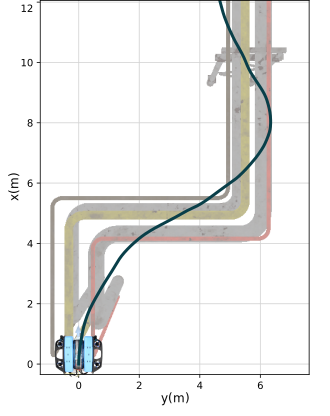
\includegraphics[width=8.4cm]{figs/paper5-unavsim/trajectory2.pdf}
    \caption[Trajectory drawn by the ROV in the DRL experiments]{Trajectory followed by the \ac{DRL} agent (dark blue) along with the pipes from the top view. The starting point is the origin of the coordinate frame and is indicated with the \ac{ROV}.
    %The  experimental results show that training the ego agent (\ac{ROV}) in a photo-realistic underwater environment can effectively enable it to be deployed in an underwater pipe inspection scenario.
    }
    \label{fig:trajectory_drl}
\end{figure}



\subsection{Visual localization benchmarking}
The vision-based trajectory generated in Section \ref{sec:example:planning}, being carried out by the robot with the controller showcased in Section \ref{sec:stack:control}, has served as a test setup for the visual localization experiment.
Two trajectories are carried out: a linear trajectory where no area in the map is revisited (see Fig. \ref{fig:trajectory_drl}), and a trajectory with a loop, where the robot navigates back to the starting point.
The benchmarking is automatically performed by the \texttt{robot\_visual\_localization} metapackage using \cite{grupp2017evo}. 

During runtime, the estimated trajectory $P_i$ and the ground truth trajectory $Q_i$ are recorded into separate files composing a sequence of time-synchronized spatial poses. The pose format is the one proposed in \cite{sturm2012tumrgbd}, composed of the three spatial coordinates with the orientation in quaternions.
The metrics implemented are the \ac{APE} and the \ac{RPE}, which are automatically deployed over the recorded trajectories before shutdown. TartanVO presents a monocular visual odometry algorithm. Therefore, for a fair comparison, the ORB-SLAM3 experiment is executed under a monocular setup. 
The deployment of monocular algorithms implies that the orientation of the algorithm's world frame and the trajectory's scale is arbitrary. Therefore, the estimated trajectories are aligned with the ground truth by obtaining the transform $S \in Sim_3$ that best aligns $P_i$ with $Q_i$.

With the deployment of the automatic stack for visual inspection proposed by UNav-Sim, benchmarking of visual localization algorithms becomes a straightforward task: the robot follows the pipeline autonomously under the planned trajectory, with the visual localization algorithms being automatically executed by the \texttt{robot\_visual\_localization} package, which on shutdown generates the results as depicted in Table \ref{unavsim:table:comparisonSLAM}. It can be seen from the generated results that the two proposed algorithms depict a similar performance in the linear trajectory, but ORB-SLAM outperforms TartanVO under the presence of a closed loop.
Despite ORB-SLAM's high efficiency in state-of-the-art datasets, the realistic underwater conditions confront one of the main challenges for feature-based approaches: the lack of texture. Moreover, the pipes are the main source of features, which avoids their uniform distribution across the image. Without enough evenly-distributed features, the ORB-SLAM's front end drifts. Nevertheless, the closed trajectory shows the convenience of the back-end's loop closure algorithm: the absolute errors are significantly reduced for translation and rotation.
On the other hand, TartanVO presents a drift similar to ORB-SLAM's in the translations, but slightly higher for rotations. These results show the great potential of learning-based algorithms under imaging conditions that challenge geometry-based methods. Although the lack of generalization ability is the main source of drift in this case, TartanVO has been trained with high amounts of diversified data that explain its good performance in the proposed setup.

In conclusion, the framework proposed in UNav-Sim has enabled the automatic benchmarking of state-of-the-art visual localisation algorithms in a realistic underwater scenario. This has allowed the challenges and opportunities of these algorithms to be easily demonstrated in a geometry-based and learning-based manner.

\begin{table}[ht!]
\centering
\footnotesize
\caption[Visual localization results in the pipeline tracking scenario]{Visual localization results in the pipeline tracking scenario.}
\label{unavsim:table:comparisonSLAM}
\begin{tabular}{cc c c c c  }
\toprule

Trajectory                   & Algorithm  & APE[m]         & RPE[m]         & APE[rad]       & RPE[rad] \\
\midrule
\multirow{2}{*}[0em]{Linear} & ORB-SLAM3  & 1.75          & \textbf{0.412} & \textbf{1.53} & \textbf{0.036} \\
                             & TartanVO   & \textbf{1.67} & 0.489          & 1.95          & 0.108 \\
\midrule
\multirow{2}{*}[0em]{With loop}   & ORB-SLAM3  & \textbf{0.078}          & 0.372 & \textbf{1.62} & \textbf{0.006} \\
                             & TartanVO   & 0.961 & \textbf{0.322}         & 2.10          & 0.068 \\
\bottomrule
\end{tabular}
\end{table}

% \begin{table}[ht!]
% \centering
% \scriptsize
% \caption{visual localization results in the pipeline tracking scenario.
% }
% \label{unavsim:table:comparisonSLAM}
% \begin{tabular}{|c| c c c c | }
% \hline

% Algorithm  & APE[m]         & RPE[m]         & APE[rad]       & RPE[rad] \\
% \hline
% ORB-SLAM3  & 1.754          & \textbf{0.412} & \textbf{1.525} & \textbf{0.036} \\
% TartanVO   & \textbf{1.667} & 0.489          & 1.952          & 0.108 \\
% \hline
% \end{tabular}
% \end{table}




\section{Conclusion \& future work} \label{sec:unavsim:conclusion}
We have developed UNav-Sim, a novel open-source underwater simulator, which builds upon AirSim and \ac{UE5} and incorporates state-of-the-art robotics algorithms. UNav-Sim also supports \ac{ROS} and multiple operating systems, facilitating a streamlined and efficient development process for robotics applications. Future work will include the incorporation of additional underwater sensors, vehicle models, and more custom environments. 




\chapter{REACT: Real-time Entanglement-Aware Coverage
Path Planning for Tethered Underwater Vehicles}
%\addcontentsline{toc}{chapter}{Paper II: REACT: Real-time Entanglement-Aware Coverage Path Planning for Tethered Underwater Vehicles}
\vspace{1cm}

This paper was submitted to the \textbf{Transactions on Field Robotics}.

 \section{Abstract}
 Inspection of complex underwater structures with tethered underwater vehicles is often hindered by the risk of tether entanglement. We propose REACT (real-time entanglement-aware coverage path planning for tethered underwater vehicles), a framework designed to overcome this
limitation. REACT comprises a fast geometry-based tether model using the signed distance field (SDF) map for accurate, real-time simulation of taut tether configurations around arbitrary structures. This model enables an efficient online replanning strategy, enforcing a maximum tether length constraint, thereby actively preventing entanglement. By integrating REACT into a coverage path planning framework, we achieve safe and optimal inspection paths, previously challenging due to tether constraints. What is more, the underlying model predictive controller (MPC) renders optimal trajectory following while accounting for system dynamics. The complete REACT framework’s efficacy is validated in a pipe inspection scenario, demonstrating safe, entanglement-free navigation and full-coverage inspection.

 \newpage
 \section{Introduction}
\label{sec:introduction}

% % Underwater Robot Applications:
%
In many applications, \Acfp{ROV} play a pivotal role, including surveying, inspection, and search-and-rescue operations, by improving efficiency and ensuring safety \cite{amer2023unav, amergp}.
%
% Why We Need Tether:
%
Most \acp{ROV} are tethered to ensure a continuous power supply during long-duration missions and to maintain reliable communication.
%
% Introducing Problem Definition:
%
However, the presence of a tether introduces complexities in path planning and control, as it poses a risk of entanglement with underwater objects such as flora, fauna, or structures being inspected.

This challenge restricts the applicability of many path planning algorithms originally designed for untethered drones and surface vehicles. For instance, numerous \ac{CPP} algorithms exist to compute distance-optimal paths for covering 3D structures \cite{bircher2015structural,feng2024fc, amer2023visual}. Additionally, exploration path planners are employed to determine the next viewpoints for mapping and exploring unknown terrains \cite{dang2020graph}. However, these methods do not account for entanglement with the surroundings and thus cannot be directly applied to tethered underwater robots.
%
% Entanglement Problem and Definition:
%
Entanglement occurs when the movement of the underwater vehicle is restricted due to physical interactions between the tether and objects in the environment. Tether can bend or loop around obstacles, limiting vehicle mobility. This work bridges a critical gap in automatic asset inspection with \ac{ROV} by proposing \ac{REACT}.

The contributions of this work can be summarized as follows:
\begin{itemize}
\item A fast online tether model that computes the tether configuration in real time using \ac{SDF} data of arbitrary underwater structures.
\item An efficient online replanning method that prevents entanglement by incorporating a maximum tether length constraint.
\item Integration of the proposed method into a coverage path planning framework with \ac{MPC} to enable optimal inspection of underwater structures while avoiding entanglement.

\item Demonstration of the complete framework in simulation, showcasing its ability to ensure safe and efficient underwater structure inspection.
\end{itemize}





%
\begin{figure}[t!]
	\centering	\includegraphics[width=0.7\linewidth]{figures/react_abstract.pdf}
	  \caption{\textcolor{black}{Overview of the \ac{REACT} inspection framework. In the offline phase, a \ac{SDF} map is generated from a point cloud, and the FC-Planner \cite{feng2024fc} computes an optimal waypoint sequence. In the online phase, a tether model $\mathbf{P}^{tether}(t)$ ensures the maximum tether length is maintained, while an \ac{MPC} controller applies the optimal wrench $\mathbf{u}(t)$ to the \ac{ROV}}.}
    \label{fig:abstract}
\end{figure}
%


The remainder of this paper is organized as follows: Section \ref{sec:related_work} reviews the state of the art. Section \ref{sec:framework} presents the path planning framework for underwater structure inspection with tether constraints. Section \ref{sec:tether_model} introduces the taut-tether model, and Section \ref{sec:planner} details the online entanglement-aware path planner. Experimental results are shown in Section \ref{sec:experiments}, followed by conclusions and future work in Section \ref{sec:conclusion}.






\section{State of the art}
\label{sec:related_work}

% Paragraph 1: Introduction to Tether Importance and Entanglement Definition
Tethers play a vital role in numerous mobile robotics applications, offering crucial power delivery and reliable data transmission. It enables extended operational periods and ensures consistent communication links for the robot. However, the risk of entanglement with obstacles represents a significant planning challenge. To systematically address this, a taxonomy of entanglement definitions has been presented in \cite{definitions}, cataloging existing interpretations from the literature and introducing new definitions, paving the way for developing new path planning strategies that account for entanglement.

% Paragraph 2: Early Approaches - 2D Offline Path Planning (Single Robot)
Initial efforts to develop entaglement-aware path planners often focused on two-dimensional environments and employed offline computation strategies. For instance, \cite{rov_mccammon} and \cite{mechsy2017novel} proposed methods for planning paths in 2D to cover a predefined set of waypoints while considering tether constraints. Notably, \cite{mechsy2017novel} formulated the path planning problem for a \ac{ROV} as a mixed-integer programming problem. Their approach first solves a \ac{TSP} to find an optimal waypoint sequence and then incorporates homotopic constraints during path generation to minimize the likelihood of tether entanglement. While effective for predefined scenarios, these offline methods lack the adaptability required for dynamic environments.

% Paragraph 3: Advancements - 2D Online Path Planning (Single Robot)
Addressing the need for real-time adaptability, subsequent research explored online path planning algorithms, still primarily in 2D. \cite{kim} introduced a homotopy-augmented topological approach combined with graph search techniques, allowing for dynamic adjustments to the path based on environmental perception. Similarly, \cite{withy} developed a hybrid A* variant that utilizes a modified tangent graph. This method efficiently plans curvature-constrained paths for tethered robots subject to winding angle constraints, demonstrating guarantees and providing simulation results for online entanglement avoidance. %These online planners represent a significant step towards real-time tether management.

% Paragraph 4: Scaling Complexity - Multi-Robot Systems in 2D
The complexity of tether management increases significantly when coordinating multiple robots. Several approaches have tackled this challenge in 2D. Early work by \cite{hert1996ties} laid groundwork in this area, followed by methods like \cite{zhang2019planning}. More recently, \cite{cao2023neptune} presented an efficient online path planner for multi-robot systems. Their method integrates a homotopy-based high-level planner with trajectory optimization and smoothing techniques to generate entanglement-free paths. However, despite its online capability, this approach remains constrained to 2D environments.

% Paragraph 5: Moving to Three Dimensions - 3D Path Planning (Single Robot)
Real-world applications frequently require navigation in 3D environments, such as with underwater robots. Consequently, work by  \cite{bhattacharya2012topological} and \cite{martinez2021optimization} explored topological aspects and optimization techniques for 3D tethered navigation. \cite{petit2022tape} specifically presented a 3D exploration path planner that incorporates explicit contact avoidance constraints for the tether, facilitating safer navigation for single tethered robots in complex three-dimensional spaces.

% Paragraph 6: 3D Multi-Robot Path Planning
 \cite{hert1999motion} extended their earlier 2D work to handle the increased complexity of 3D multi-robot scenarios. Further advancements by \cite{patil2023coordinating} and  \cite{cao2023path} introduced path planning strategies that explicitly consider the topological constraints imposed by multiple interacting tethers in 3D. While these methods advance the state-of-the-art in multi-robot coordination, they are generally designed for offline computation and are not suited for online path planning where real-time implementation is essential.

% Paragraph 7: Identifying the Research Gap
% Summarize the limitations of existing work: 
In summary, existing tether-aware planners often face limitations for practical online coverage path planning (CPP) in complex 3D settings. Many are too computationally intensive for real-time use \cite{mechsy2017novel, hert1999motion, patil2023coordinating, cao2023path}, lack integrated tether-aware CPP frameworks, or rely on simplifying assumptions like 2D environments or basic obstacle shapes \cite{kim, withy, cao2023neptune}, hindering generalization to real-world inspection tasks.
% Paragraph 8: Introducing the Proposed Solution (REACT) based on its key contributions
To address these limitations, we propose \ac{REACT}, a novel approach that enables real-time, entanglement-aware path planning in arbitrary 3-D environments.


% --- End of Literature Review Section ---













































% % Introduce tether in literature
% Tether considerations in autonomous robot planning has drawn increasingly attention in robotics literature due to their critical role in enabling robots to operate autonomously in unknown environments for a wide range of mobile robots. 
% % Entaglement definitions
% A taxonomy of entanglement definitions is presented in \cite{definitions} which catalogs existing definitions from the literature and also introduces six new definitions.  These definitions open the door to the design of new entanglement aware path planning approaches.

% % 2-D , offline
% Regarding the path planners, many path planning methods have been proposed to address tether entanglement in 2-D environments. \cite{rov_mccammon} and \cite{mechsy2017novel} propose 2-D offline path planning to cover a set a way-points. In particular, \cite{mechsy2017novel} formulate the path planning problem for a \ac{ROV} as a mixed-integer programming problem. Their method solves a \ac{TSP} to determine the optimal sequence of waypoint visits, while incorporating homotopic constraints to reduce the likelihood of tether entanglement.
% % 2-D , online
% Also in 2-D, but in an online fashion, a homotopy-augmented topological approach, combined with graph search techniques is proposed by \cite{kim}. In addition to offline methods, online path planners allow real-time entanglement avoidance \cite{kim}, \cite{withy}. A hybrid A* variant uses a modified tangent graph to efficiently plan curvature-constrained, tethered robot paths under winding angle constraints, with guarantees and simulation results provided \cite{withy}.
% % 2-D , Multirobot
% Other approaches, also in 2-D address the tether constraints problem for the multi-robot case in \cite{zhang2019planning}, \cite{hert1996ties}, and \cite{cao2023neptune}. An efficient online path planner is presented in \cite{cao2023neptune}, combining a homotopy-based high-level planner with trajectory optimization and smoothing to generate entanglement-free paths for multi-robot systems. However, this approach is limited to 2-D environments. 
% % 3-D , Multirobot
% Entanglement avoidance has also been investigated in 3-D environments, as demonstrated in \cite{petit2022tape}, \cite{martinez2021optimization}, and \cite{bhattacharya2012topological}. In particular, \cite{petit2022tape} presents a 3-D exploration path planner that incorporates contact avoidance constraints on the tether, enabling safe navigation for tethered robots in three-dimensional spaces. For multi-robot operations, \cite{hert1999motion} extends earlier work to handle the increased complexity of coordinating multiple tethered robots. Further advancements by \cite{patil2023coordinating} and \cite{cao2023path} introduce improved coordination strategies that consider topological constraints imposed by multiple tethers. However, these approaches are not designed for real-time, online path planning.

% % NICHE and summary of research gap 
% In summary, most existing planners suffer from limitations that hinder their use in practical, online coverage path planning applications. Many are too computationally intensive for real-time implementation, and there is a lack of coverage path planning frameworks that explicitly account for the tether during planning. Existing tether-aware methods often rely on simplifying assumptions, such as 2-D environments or simplistic obstacle shapes (e.g., circles or cylinders), and thus fail to generalize to complex, real-world environments—particularly in inspection tasks.
% % Introduce REACT
% To address these limitations, we propose \ac{REACT}, a novel approach that enables real-time, entanglement-aware path planning in arbitrary 3-D environments.




\section{Overall \ac{REACT}  Framework}
\label{sec:framework}
\ac{REACT} framework, as depicted in \ref{fig:abstract}, consists of two main components: an offline planning phase and an online execution phase. In the offline phase, the environment is provided as a point cloud, including the object to be inspected. A \ac{SDF} map is then generated from this point cloud using the nvblox library \cite{nvblox}. The extracted point cloud of the structure to be inspected is then processed by the FC-Planner \cite{feng2024fc} to compute an optimal ordered sequence of waypoints, to acheive a path that performs full inspection coverage, initially disregarding tether constraints.

%Online Phase
In the online phase, tether constraints are handled by a entanglement-aware re-planner that ensures that the maximum tether length is not exceeded due to entanglement. This is achieved using our developed tether model, which continuously updates based on the current state of the tether and the new position of the \ac{ROV}, denoted as $\textbf{p}_{rov}$. The online planner then provides the reference state to an \ac{MPC} controller, which computes and applies the optimal wrench (forces and torques) to the \ac{ROV}.



%%%%%%%%%%%%%%%%%%%%%
%%%%%%  Tether Figure  
%%%%%%%%%%%%%%%%%%%%%

\begin{figure*}[t!]
    \centering
    \includegraphics[width=1\linewidth]{Phd_thesis/figures/tether_model.pdf}
    \caption{Tether shortcutting during \ac{ROV} motion from \( t_1 \) to \( t_2 \). (1) Initial tether with new \ac{ROV} position \( \mathbf{p}_{\text{rov}} \) appended; (2) Successful shortcut from the end node; (3) Collision encountered when attempting further shortcutting, prompting move to the next node; (4) Another collision detected from the new node; (5) Successful shortcut from a subsequent node; (6) Final tether configuration (yellow) after applying all feasible shortcuts.}
    \label{fig:tether}
\end{figure*}
%%%%%%%%%%%%%%%%%%%%%%%%



%%%%%%%%%%%%%%%%%%%%%%%%%%%
%%%%%%%%%%%%%%%%%%%%%%%%%%%
%%%%%% Tether Model Section
%%%%%%%%%%%%%%%%%%%%%%%%%%%
%%%%%%%%%%%%%%%%%%%%%%%%%%%
\section{Tether Model}
\label{sec:tether_model}
In this section, we introduce a computationally efficient kinematic \ac{ROV} tether model. Inspired by the shortcutting algorithm used in the ropeRRT path planner \cite{roperrt}, which simplifies sampled trajectories in a manner analogous to a rope tightening around an obstacle. The key assumption in the proposed model is that we assume a geometry-based constraint where the tether remains taut and fully stretched at all times.

\subsection{Tether model description}
Let the tether path at time \( t \) be denoted by \( \mathbf{P}^{tether}(t) = \{ p_i(t) \}_{i=1}^{N} \), where each node \( p_i(t) \in \mathbb{R}^3 \) represents the position of the \( i \)-th node in 3D space at time \( t \), and \( N \) is the total number of nodes in the tether path. The position of the ROV at time \( t \), denoted by \( \mathbf{p}_{rov}(t) \in \mathbb{R}^3 \), is appended \( p_{N+1}(t) \) at the end of the tether path, ensuring that the ROV's position is included in the configuration. 

The proposed tether model iteratively optimizes the tether path via two main mechanisms: shortcutting and pulling. For each pair of nodes \( (p_i(t), p_j(t)) \) where \( i < j \), the algorithm attempts to shortcut the path segment between them. If the line of sight between \( p_i(t) \) and \( p_j(t) \) is collision-free, determined via a \ac{SDF} map \( \mathcal{M}_{sdf} \), the intermediate nodes are replaced with a straight segment sampled at a resolution \( \delta_n \).





%%%%%%%%%%%%%%%%%%%%%%%%%%%%%%%%%%%%%%%%%%
%%%%%%  Tether Model Algorithm  %%%%%%%%%
%%%%%%%%%%%%%%%%%%%%%%%%%%%%%%%%%%%%%%%%%%


\begin{algorithm}[H]
%\SetAlgoLined
\LinesNotNumbered  % Disable line numbers

\SetKwInOut{Input}{Require}
\SetKwInOut{Output}{Return}
\Input{
ROV position $\mathbf{p}_{rov}(t)$, 
Tether path $\mathbf{P}^{tether}(t)$, 
SDF map $\mathcal{M}_{sdf}$, 
parameters: $\delta_{n}$
}
\Output{Taut-tether at $t+1$ : $\mathbf{P}^{tether}(t+1)$}
\BlankLine

\tcp{Extend tether path to include the current ROV position as the endpoint}
Append $\mathbf{p}_{rov}(t)$ to $\mathbf{P}^{tether}(t).end()$\;

%\tcp{Iterative shortcutting path segments by skipping intermediate nodes}
\tcp{Iterative shortcutting}
\For{$i \gets len(\mathbf{P}^{tether}(t)) - 2$ \textbf{to} $1$}{
    \For{$j \gets i+1$ \textbf{to} $len(\mathbf{P}^{tether}(t)) - 1$}{
        \tcp{Check if shortcutting the path is valid between nodes $i$ and $j$}
        \If{checkshortcut($\mathbf{P}^{tether}(t), i, j$)}{
            \tcp{Replace intermediate nodes $i-j$ }
            ReplaceIntermediateNodes($\mathbf{P}^{tether}(t)$, $i$, $j$, $\delta_{n}$)\;
        }
        \Else{
            \If{not CheckLineOfSight($\mathcal{M}_{sdf}$, $\mathbf{P}^{tether}(t)$)}{
                \tcp{Line of sight is blocked by obstacle, stop shortcutting}
                \textbf{break}\;
            }
            \If{isInCollision($\mathcal{M}_{sdf}$, $\mathbf{P}^{tether}(t)[j]$)}{
                \tcp{Pull node towards tether end}
                PullNode($\mathbf{P}^{tether}(t)[j]$, $\mathbf{P}^{tether}(t).end()$, $\delta_{n}$)\;
            }
        }
    }
}
\Return{$\mathbf{P}^{tether}(t+1)$}\;
\caption{Taut-Tether Model}
\label{alg:tether_optimization}
\end{algorithm}



%%%%%%%%%%%%%%%%%%%%%%%%%%%
%%%%%%%%%%%%%%%%%%%%%%%%%%%
% Homotopy equivelance proof
%%%%%%%%%%%%%%%%%%%%%%%%%%%
%%%%%%%%%%%%%%%%%%%%%%%%%%%


% \subsection{Homotopic Equivalence of the Shortcutting-Based Tether Path}
% \label{sec:homotopy_proof}

% In this subsection, we demonstrate that the taut-tether path generated primarily through the shortcutting mechanism is homotopically equivalent to the Remotely Operated Vehicle's (ROV) actual trajectory. This argument focuses on the geometric simplification provided by shortcutting, assuming the tether behaves like a rope tightening around obstacles.

% \subsubsection{Preliminaries and Definitions}
% Let the ambient Euclidean space be $X = \mathbb{R}^3$. The static obstacle region, $O \subset X$, is a closed set. The \textbf{free configuration space} is defined as $C_{free} = X \setminus O$. A \textbf{path} in $C_{free}$ is a continuous function $\gamma: [0,1] \to C_{free}$.

% Two paths $\gamma_0, \gamma_1: [0,1] \to C_{free}$ sharing the same endpoints (i.e., $\gamma_0(0)=\gamma_1(0)$ and $\gamma_0(1)=\gamma_1(1)$) are said to be \textbf{homotopic in $C_{free}$} (denoted $\gamma_0 \sim \gamma_1$) if there exists a continuous function $H: [0,1] \times [0,1] \to C_{free}$, called a \textbf{homotopy}, such that:
% \begin{itemize}
%     \item $H(s,0) = \gamma_0(s)$ for all $s \in [0,1]$,
%     \item $H(s,1) = \gamma_1(s)$ for all $s \in [0,1]$,
%     \item $H(0,\tau) = \gamma_0(0)$ for all $\tau \in [0,1]$ (startpoints fixed),
%     \item $H(1,\tau) = \gamma_0(1)$ for all $\tau \in [0,1]$ (endpoints fixed).
% \end{itemize}
% Let $p_A \in C_{free}$ denote the fixed anchor point of the tether and $p_R(t) \in C_{free}$ be the ROV's position at time $t$. The actual continuous trajectory of the ROV up to time $t$ is a path $\Gamma_{ROV}: [0,1] \to C_{free}$, with $\Gamma_{ROV}(0) = p_A$ (assuming the path starts at the anchor for simplicity) and $\Gamma_{ROV}(1) = p_R(t)$.

% A \textbf{piecewise linear (PL) path}, $\mathbf{P}$, connecting $p_A$ to $p_R(t)$ is defined by an ordered sequence of $N+1$ vertices $(v_0, v_1, \ldots, v_N)$ where $v_0=p_A$, $v_N=p_R(t)$, and each $v_k \in C_{free}$. The path consists of line segments $L(v_k, v_{k+1}) = \{ (1-s)v_k + s v_{k+1} \mid s \in [0,1] \}$. For $\mathbf{P}$ to be a path in $C_{free}$, each segment $L(v_k, v_{k+1})$ must be entirely contained in $C_{free}$.

% \subsubsection{Initial Tether Path and Shortcutting as a Homotopy}
% Let $\mathbf{P}_{init}(t)$ be an initial PL path representing the tether before shortcutting optimization at time $t$. This path connects $p_A$ to $p_R(t)$ and is assumed to be a PL approximation of $\Gamma_{ROV}$ lying in $C_{free}$. It is a standard result in algebraic topology that $\Gamma_{ROV} \sim \mathbf{P}_{init}(t)$ if $\mathbf{P}_{init}(t)$ is a sufficiently fine approximation.

% The shortcutting mechanism iteratively refines a PL path. Let $\mathbf{P}_{k} = (v_0, \ldots, v_M)$ be the PL tether path at iteration $k$. A shortcutting step selects two non-consecutive vertices $v_i, v_j \in \mathbf{P}_{k}$ (where $i < j-1$). Let $\sigma_{old}$ be the subpath of $\mathbf{P}_{k}$ from $v_i$ to $v_j$, and let $\sigma_{new}$ be the straight-line segment $L(v_i, v_j)$. If $\sigma_{new} \subset C_{free}$ (i.e., the line of sight is collision-free), the path $\mathbf{P}_{k+1}$ is formed by replacing $\sigma_{old}$ with $\sigma_{new}$.

% \textbf{Claim:} If $\sigma_{new} \subset C_{free}$, then $\sigma_{old} \sim \sigma_{new}$ in $C_{free}$ relative to their common endpoints $v_i$ and $v_j$.

% \textit{Proof of Claim:}
% The tether model is "analogous to a rope tightening around an obstacle." When a flexible rope segment, initially following $\sigma_{old} \subset C_{free}$, is pulled taut between $v_i$ and $v_j$, and the direct path $\sigma_{new}$ is also in $C_{free}$, the rope physically deforms into $\sigma_{new}$ by moving exclusively through $C_{free}$.
% This continuous deformation can be represented by a homotopy. Let $\sigma_{old}(s)$ parameterize the PL path $\sigma_{old}$ for $s \in [0,1]$, and $\sigma_{new}(s) = (1-s)v_i + s v_j$ parameterize the segment $\sigma_{new}$. A straight-line homotopy is $H(s, \tau) = (1-\tau)\sigma_{old}(s) + \tau\sigma_{new}(s)$ for $s, \tau \in [0,1]$.
% The "rope tightening" analogy implies that if $\sigma_{new} \subset C_{free}$, then the entire region swept by the deformation from $\sigma_{old}$ to $\sigma_{new}$ is also contained in $C_{free}$. Thus, $H(s, \tau) \in C_{free}$ for all $s, \tau$. This ensures that $\sigma_{old} \sim \sigma_{new}$ in $C_{free}$.
% Since $\mathbf{P}_{k+1}$ is obtained from $\mathbf{P}_{k}$ by substituting $\sigma_{old}$ with a homotopic segment $\sigma_{new}$, it follows that $\mathbf{P}_{k} \sim \mathbf{P}_{k+1}$.
% \hfill $\qed$

% \subsubsection{Iterative Application and Final Equivalence}
% The shortcutting algorithm generates a sequence of PL paths $\mathbf{P}_{init}(t) = \mathbf{P}_0, \mathbf{P}_1, \ldots, \mathbf{P}_{final}$, where $\mathbf{P}_{final}$ is the resulting taut-tether path, denoted $\mathbf{P}^{tether}(t)$. Since each step is a homotopy, $\mathbf{P}_0 \sim \mathbf{P}_1 \sim \ldots \sim \mathbf{P}_{final}$. By the transitivity of the homotopy relation, $\mathbf{P}_{init}(t) \sim \mathbf{P}^{tether}(t)$.

% Given that $\Gamma_{ROV} \sim \mathbf{P}_{init}(t)$, and $\mathbf{P}_{init}(t) \sim \mathbf{P}^{tether}(t)$, we conclude by transitivity that:
% $$ \Gamma_{ROV} \sim \mathbf{P}^{tether}(t) $$
% Thus, the taut-tether path $\mathbf{P}^{tether}(t)$, resulting from the shortcutting operations, is homotopically equivalent to the ROV's actual trajectory $\Gamma_{ROV}$ within the free configuration space $C_{free}$. The shortcutting process simplifies the path to a tighter representative within its original homotopy class with respect to the obstacles.



%%%%%%%%%%%%%%%%%%%%%%%%%%%%%%%%%%%%%%%%%%
%%%%%%%%%%%%%%%%%%%%%%%%%%%%%%%%%%%%%%%%%%
%%%%%%%%%%%%%%%%%%%%%%%%%%%%%%%%%%%%%%%%%%


If the shortcut is obstructed or the endpoint node \( p_j(t) \) is in collision, the model applies a pulling operation. This simulates disentanglement by moving \( p_j(t) \) incrementally toward the tether endpoint \( p_{N+1}(t) \), ensuring the new configuration remains collision-free. This iterative process continues until no further shortcuts or pulling is possible, resulting in an updated, taut, and obstacle-free tether path \( \mathbf{P}^{tether}(t+1) \). An example of the shortcut operation is illustrated in Fig.~\ref{fig:tether}.


% %%%%%%%%%%%%%%%%%%%%%%%%%%%
% %%%%% REACT Planner %%%%%%
% %%%%%%%%%%%%%%%%%%%%%%%%%%%
\begin{algorithm}[H]
\LinesNotNumbered  % Disable line numbers

\SetKwInOut{Input}{Input}
\SetKwInOut{Output}{Return}
\Input{
Waypoints $\mathbf{W}$, 
Maximum tether length $L_{\max}$, 
Current tether configuration $\mathbf{P}^{tether}(t)$, 
Current ROV position $\mathbf{p}_{\text{rov}}(t)$, 
Current waypoint index $k$, $d_{thresh}$}

\Output{Target point for controller $\mathbf{p}_{\text{target}}$}
\BlankLine

Compute $L_{\text{tether}}(t)$ 

\If{$L_{\text{tether}}(t) > L_{\max}$ \textbf{and not} finding\_safe\_path}{
    finding\_safe\_path $\gets$ True\; \tcp{Activate recovery mode}
    $\mathbf{P}_{\text{recovery}} \gets \text{SearchAlternativePath}(\mathbf{P}^{tether}(t), \mathbf{W}[k], L_{\max})$\; \tcp{Find path within tether limits}
    $\mathbf{P}_{\text{safe}} \gets \text{RefineRecoveryPath}(\mathbf{P}_{\text{recovery}})$\; %\tcp{Optimize the recovery path}
    path\_is\_safe $\gets \text{CheckPathValidity}(\mathbf{P}_{\text{safe}})$\; \tcp{Check if recovery path is valid}
    safe\_path\_index $\gets 0$\; \tcp{Start from the beginning of the recovery path}
}

\If{finding\_safe\_path \textbf{and} path\_is\_safe}{
    $\mathbf{p}_{\text{target}} \gets \text{GetPointAlongPath}(\mathbf{P}_{\text{safe}}, \text{safe\_path\_index})$\; \tcp{Get target from recovery path}
    \If{$\|\mathbf{p}_{\text{rov}}(t) - \mathbf{p}_{\text{target}}\| < d_{thresh}$}{
        safe\_path\_index $\gets$ safe\_path\_index + 1\; \tcp{Advance to next point}
    }
    \If{safe\_path\_index $\ge$ $|\mathbf{P}_{\text{safe}}|$}{
        finding\_safe\_path $\gets$ False\; \tcp{Recovery complete}
        $\mathbf{p}_{\text{target}} \gets \mathbf{W}[k]$\; \tcp{Resume wp tracking}
    }
}
\Else{
    finding\_safe\_path $\gets$ False\; \tcp{Reset recovery}
    $\mathbf{p}_{\text{target}} \gets \mathbf{W}[k]$\; \tcp{Default to current wp}

    \If{$\|\mathbf{p}_{\text{rov}}(t) - \mathbf{p}_{\text{target}}\| < d_{thresh}$}{
         $k \gets k + 1$\; \tcp{Advance to next wp}
    }
}
\Return{$\mathbf{p}_{\text{target}}$}\;
\caption{Real-time Entanglement-Aware Path Planning}
\label{alg:main_loop}
\end{algorithm}


%%%%%%%%%%%%%%%%%%%%%%%%%%%%%%%%%
%% Alg. 3 Recovery Path  Algorithm %%%
%%%%%%%%%%%%%%%%%%%%%%%%%%%%%%%%%

\begin{algorithm}[t]
\LinesNotNumbered  % Disable line numbers
\SetKwInOut{Input}{Require}
\SetKwInOut{Output}{Return}
\Input{
Current tether $\mathbf{P}(t)$,
Goal waypoint $\mathbf{p}_{\text{goal}}$,
Maximum length $L_{\max}$
}
\Output{Recovery path segment $\mathbf{P}_{\text{recovery}}$}
\BlankLine
best\_path $\gets$ None\;
prev\_len $\gets \infty$\;
found\_suitable $\gets$ False\;
\For{$i \gets |\mathbf{P}(t)| - 3$ \textbf{downto} 3}{
    $\mathbf{P}_{\text{candidate}} \gets \text{GeneratePath}(i, \mathbf{P}(t), \mathbf{p}_{\text{goal}})$\;
    $L_{\text{candidate}} \gets \text{ComputeLength}(i, \mathbf{P}(t), \mathbf{P}_{\text{candidate}})$\;\\
    \If{$L_{\text{candidate}} < 0.7L_{\max}$} %\textbf{and} $L_{\text{candidate}} < 0.65 \cdot \text{prev\_len}$}
    {
         best\_path $\gets \text{ExtractSegment}(i+2, \mathbf{P}(t))$\;
         found\_suitable $\gets$ True\;
         \textbf{break}\;
    }
    prev\_len $\gets \text{ComputeLength}(i-3, \mathbf{P}(t), \text{GeneratePath}(i-3, \mathbf{P}(t), \mathbf{p}_{\text{goal}}))$\;
}
\If{\textbf{not} found\_suitable}{
    $\mathbf{p}_{\text{rov}} \gets \mathbf{P}(t)[|\mathbf{P}(t)|-1]$\; \tcp{Fallback}
    $\mathbf{P}_{\text{recovery}}$ $\gets \text{PlanShortestPath}(\mathbf{p}_{\text{rov}}, \mathbf{p}_{\text{goal}})$\;
}
\Return{$\mathbf{P}_{\text{recovery}}$}\;
\caption{Search Alternative Recovery Path}
\label{alg:search_alternative}
\end{algorithm}

%%%%%%%%%%%%%%%%%%%%%%%%%%%%%%%%%%%%%%%%%%
%%%%%%%%%%%%%%%%%%%%%%%%%%%%%%%%%%%%%%%%%%
%%%%%%%%%%%%%%%%%%%%%%%%%%%%%%%%%%%%%%%%%%



%%%%%%%%%%%%%%%%%%%%%%%%%%%
%% Refine Path  Algorithm
%%%%%%%%%%%%%%%%%%%%%%%%%%%
\begin{algorithm}[b]
\LinesNotNumbered  % Disable line numbers
\SetKwInOut{Input}{Input}
\SetKwInOut{Output}{Return}
\Input{
    Recovery path $\mathbf{P}_{\text{recovery}}$;\\
    Offset distance $\delta_{\text{offset}}$;\\
    Sampling distance $\delta_{\text{sample}}$
}
\Output{Refined safe path $\mathbf{P}_{\text{safe}}$}
\BlankLine
$\mathbf{P}_{\text{offset}} \gets \text{TetherPathOffset}(\mathbf{P}_{\text{recovery}}, \delta_{\text{offset}})$\;
\\
$\mathbf{P}_{\text{sampled}} \gets \text{PerturbTetherPath}(\mathbf{P}_{\text{offset}}, \delta_{\text{sample}})$\;
\\
$\mathbf{P}_{\text{safe}} \gets \text{SmoothTetherPath}(\mathbf{P}_{\text{sampled}})$\;
\\
\Return{$\mathbf{P}_{\text{safe}}$}\;
\caption{Refine Recovery Path}
\label{alg:refine_path}
\end{algorithm}


%%%%%%%%%%%%%%
%%%%%%%%%%%%%%
%%%%%%%%%%%%%%

%%%%%%%%%%%%%%%%%%%%%%%%%%%
%%%%%%%%%%%%%%%%%%%%%%%%%%%
%%%%%%% PLANNER %%%%%%%%%
%%%%%%%%%%%%%%%%%%%%%%%%%%
%%%%%%%%%%%%%%%%%%%%%%%%%%





\section{Real-Time Entanglement-Aware Path Planner}
\label{sec:planner}

In this section, we present the real-time entanglement-aware path planner, a local planner designed to handle real-time entanglement-free path finding for autonomous system navigating operating with a tether. The planner runs in an online manner, continuously monitoring the tether configuration and adapting the \ac{ROV}'s path to avoid exceeding the maximum allowable tether length, \( L_{\text{max}} \), while ensuring safe, collision-free motion towards a sequence of reference waypoints.

At each time step \( t \), the planner utilizes the current estimated tether configuration  $\mathbf{P}^{tether}(t)$. The planner also maintains a list of reference waypoints \( \mathbf{W} = \{\mathbf{p}_{\text{waypoint}}(k)\}_{k=1}^{M} \), where \( \mathbf{p}_{\text{waypoint}}(k) \in \mathbb{R}^3 \) denotes the \( k \)-th target waypoint. The current tether length \( L_{\text{tether}}(t) \) is computed by summing the Euclidean distances between consecutive tether points, i.e., \( L_{\text{tether}}(t) = \sum_{i=1}^{N-1} \| p_i(t) - p_{i+1}(t) \| \), and is subsequently compared to the predefined maximum allowable length \( L_{\text{max}} \), to activate the re-planner.

\subsection{Nominal Operation}
If the tether length constraint is satisfied, i.e., \( L_{\text{tether}}(t) \leq L_{\text{max}} \), the planner operates in its nominal mode. It identifies the next reference waypoint \( \mathbf{p}_{\text{waypoint}}(k) \) from the list \( \mathbf{W} \) that has not yet been reached and directs the \ac{ROV} controller towards it. The system proceeds sequentially through the waypoints as long as the tether constraint remains satisfied.



\subsection{Entanglement Avoidance Strategy}
If the tether length exceeds the maximum allowable limit, \( L_{\text{tether}}(t) > L_{\text{max}} \), the entanglement avoidance strategy is activated. This strategy aims to guide the \ac{ROV} along a temporary recovery path to de-tangle the tether before resuming navigation towards the original target waypoint.

The planner initiates a search for a suitable recovery path by iteratively evaluating potential de-tangle paths based on the current tether configuration \( \mathbf{P}^{tether}(t) \). Starting from the \ac{ROV}'s end of the tether (node \( p_{N-1}(t) \)) and moving backward towards the anchor point \( p_1(t) \), the planner considers each node \( p_i(t) \) as a potential pivot point. For each \( i \), a candidate alternative trajectory is implicitly generated, consisting of the segment from the \ac{ROV} back to \( p_i(t) \) followed by a newly planned path segment from \( p_i(t) \) to the current target waypoint \( \mathbf{p}_{\text{waypoint}}(k) \). The planner computes the estimated length of this candidate alternative tether configuration.

A recovery path is selected based on length criteria: the planner seeks a pivot point \( p_i(t) \) such that the corresponding alternative path length is significantly shorter than \( L_{\text{max}} \) (e.g., \( < 0.7 L_{\text{max}} \)) and offers substantial improvement compared to alternatives generated using nearby pivot points (e.g., \( p_{i-3}(t) \)). Once such an index \( i \) is found, the recovery path segment \( \mathbf{P}_{\text{recovery}} \) is defined as the portion of the current tether from the \ac{ROV} back to a point slightly further back along the tether, specifically \( p_{i+2}(t) \). This segment represents the initial trajectory the \ac{ROV} must follow to begin resolving the entanglement. If no suitable recovery path is found during the backward search, a direct path from the \ac{ROV}'s current position to the goal waypoint is generated as a fallback. This recovery path search process is illustrated in Fig. \ref{fig:planner_search}.  










\subsection{Recovery Path Refinement and Execution}
The initially selected recovery path \( \mathbf{P}_{\text{recovery}} \) undergoes further refinement to enhance safety and smoothness before execution. This involves several steps:
\begin{enumerate}
    \item \textbf{Centroid Offsetting:} Points along \( \mathbf{P}_{\text{recovery}} \) are pushed slightly outwards, away from the path's geometric centroid, to increase clearance from potential obstacles near the path's center.
    \item \textbf{Random Sampling Perturbation:} Points are locally perturbed by sampling in random directions, seeking nearby collision-free states to potentially escape minor constraint violations or local minima.
    \item \textbf{Polynomial Smoothing:} A polynomial function (e.g., 3rd order) is fitted to segments of the path to generate a smoother trajectory, reducing sharp turns and improving dynamic feasibility.
\end{enumerate}
The resulting refined path is denoted as \( \mathbf{P}_{\text{safe}} \). The planner then checks if \( \mathbf{P}_{\text{safe}} \) is collision-free using the state validity checker. If the entanglement strategy is active and \( \mathbf{P}_{\text{safe}} \) is valid, the controller is directed to follow points sequentially along \( \mathbf{P}_{\text{safe}} \). Once the \ac{ROV} reaches the end of \( \mathbf{P}_{\text{safe}} \), the entanglement avoidance strategy is deactivated, and the planner reverts to nominal operation, targeting the next waypoint from the original list \( \mathbf{W} \). If \( \mathbf{P}_{\text{safe}} \) is found to be invalid (e.g., due to collisions introduced during refinement), the system continues targeting the original waypoint \( \mathbf{p}_{\text{waypoint}}(k) \), relying on lower-level collision avoidance or requiring further planning cycles. 

The core logic can be summarized in the following algorithms. Algorithm~\ref{alg:main_loop} outlines the main planning cycle, Algorithm~\ref{alg:search_alternative} details the search for the recovery path, and Algorithm~\ref{alg:refine_path} describes the path refinement process.














%%%%%%%%%%%%%%%%%%%%%%%%%%%%%%%%%%%%%%%%%%
%%%%%%%%%%%%%%%%%%%%%%%%%%%%%%%%%%%%%%%%%%
%%%%%%%%%%%%%%%%%%%%%%%%%%%%%%%%%%%%%%%%%%












%%%%%%%%%%%%%%%%%%%%%%%%%
%%%% Figure : Planner search 
%%%%%%%%%%%%%%%%%%%%%%%%
%%%%%%%%%%%%%%%%%%%%%%%%
\begin{figure*}[t!]
    \centering
    \includegraphics[width=\textwidth]{Phd_thesis/figures/planner.pdf}
    \caption{Recovery path search process: 
    (1) Following the path from node \( \mathbf{p}_3 \), denoted as \( \mathbf{P}_{r_3} \), causes the tether length \( L_{\text{tether}} \) to exceed the maximum allowed length \( L_{\text{max}} \); 
    (2) a backward recovery search is initiated from node \( \mathbf{p}_2 \) along the tether trajectory \( \mathbf{P}_{tether}(t) \), but the resulting path yields no improvement in tether length; 
    (3) continuing the search further back to node \( \mathbf{p}_1 \) leads to a feasible path and an updated, valid tether configuration; 
    (4) the final planned safe path \( \mathbf{P}_{safe} \) (green) satisfies the tether constraint (\( L_{\text{tether}} \leq L_{\text{max}} \)), ensuring an entanglement-free configuration.}
    \label{fig:planner_search}
\end{figure*}
%%%%%%%%%%%%%%%%
%%%%%%%%%%%%%%%%

\section{Experiments}
\label{sec:experiments}

% one point to discuss about teher length, extends operaion.
% dsicussion on how to define maximum tether length to entaglement.
% What is the common operational tether length in industry? 
%cost benefit analysis for tether saving vs time saving

% when comaping planner compare them relative to each other percentage

% Mention that after inspection, we need to deantgale so this will take time for CPP 

%Mention that this scaled model sceanrio 

%
%Offline vs online discussion
%

%online allows for arbitrary fixation.

% allows for suggestion for remotely 

% can be emebeded in offline planer

% Run one more shape for simulations.

% Add detangeling operaton.

This section presents the experimental results of our proposed \ac{REACT} method. The entire framework is implemented in C++ to ensure computational efficiency, and integrated with ROS to facilitate modularity and ease of deployment on real-world robotic systems. For the planning component, we utilize the \ac{OMPL} library \cite{ompl} to compute shortest paths using the RRT* algorithm.  


\subsection{Experimental Set Up}
The path planner is implemented for a BlueROV2 simulation model. A \ac{MPC} approach is chosen to account for model constraints and to provide the optimal control input $\mathbf{u}^{ref} \in \mathbb{R}^4$, where $\mathbf{u}^{ref} = [F_x, F_y, F_z, M_z]^T$ represents the forces in the $X$, $Y$, and $Z$ directions, and the moment about the $Z$-axis. The goal is to follow the desired reference trajectory $\mathbf{x}^{ref} \in \mathbb{R}^6$, where $\mathbf{x}^{ref} = [x_{ref}, y_{ref}, z_{ref}, \psi_{ref}]^T$ contains the reference position ($x_{ref}$, $y_{ref}$, $z_{ref}$) and the reference yaw angle $\psi_{ref}$.

The entanglement-aware path planner provides $\mathbf{x}^{ref}$ in real time, ensuring the BlueROV2 avoids obstacles while following the desired trajectory. For further details about the controller and model, the reader is referred to \cite{amergp}.

%\subsection{Results}
We perform a comparative analysis of the proposed \ac{REACT} method and a baseline conventional \ac{CPP} (FC-Planner \cite{feng2024fc}), which does not contain explicit entanglement handling. Both planners were tested in the same simulated pipe environment.

The simulation setup consists of a pipe structure represented by an underwater pipe model from \cite{feng2024fc}. The simulated onboard camera featured a horizontal field of view of 70 degrees and a vertical field of view of 60 degrees, with a maximum inspection range of 3.0 meters. The tether constraint was defined by a maximum allowable tether length of $L_{max}$ = 10.0 meters.

Environmental coverage was evaluated geometrically. At each subsampled time step, the position and orientation of the camera were used to determine which triangles in the environment mesh were visible. A triangle was marked as visible if its centroid was within the inspection range, its surface normal faced the camera, and its projection lay within the camera's field of view. Over time, the set of all uniquely observed triangles was accumulated. The coverage at time $t$ was defined as the ratio of the number of unique visible triangles up to time $t$ to the total number of triangles in the environment.


\subsection{Results}

The quantitative performance metrics for both planners are summarized in Table~\ref{tab:performance_metrics}.

\begin{table}[ht]
    \centering
    \caption{Performance Metrics Comparison}
    \label{tab:performance_metrics}
    \resizebox{\columnwidth}{!}{%
    \begin{tabular}{|l|c|c|c|}
        \hline
        \textbf{Planner} & \textbf{Total Time (s)} & \textbf{Tether Exceeded (s)} & \textbf{Final Coverage (\%)} \\
        \hline
        \ac{REACT} & 546.00 & 93.12 & 99.91 \\
        CPP  & 429.00 & 96.58 & 99.82 \\
        \hline
    \end{tabular}%
    }
    \vspace{0.5em}
\end{table}


Figures~\ref{fig:coverage_vs_time} and~\ref{fig:tether_vs_time} visualize the performance of the planners in terms of environmental coverage and tether length, respectively.

\begin{figure}[ht]
    \centering
    \begin{subfigure}[b]{0.48\linewidth}
        \centering
        \includegraphics[width=\linewidth]{figures/coverage_vs_time.pdf}
        \caption{Environmental Coverage vs. Time for both planners.}
        \label{fig:coverage_vs_time}
    \end{subfigure}
    \hfill
    \begin{subfigure}[b]{0.48\linewidth}
        \centering
        \includegraphics[width=\linewidth]{figures/tether_length_vs_time.pdf}
        \caption{Tether Length vs. Time, highlighting the 10.0m maximum limit.}
        \label{fig:tether_vs_time}
    \end{subfigure}
    \caption{Comparison of coverage and tether behavior over time.}
    \label{fig:coverage_tether_sidebyside}
\end{figure}


\begin{figure}[ht]
    \centering
    \begin{subfigure}[b]{0.48\linewidth}
        \centering
        \includegraphics[width=\linewidth]{figures/fc_planner_final_view.pdf}
        \caption{3-D plot CPP.}
        \label{fig:3d_cpp}
    \end{subfigure}
    \hfill
    \begin{subfigure}[b]{0.48\linewidth}
        \centering
        \includegraphics[width=\linewidth]{figures/ta_planner_final_view.pdf}
        \caption{3-D plot, \ac{REACT}.}
        \label{fig:3d_oea}
    \end{subfigure}
    \caption{3D views of final trajectories. (a) CPP results in entangled tether geometry. (b) \ac{REACT} yields a non-entangled tether configuration, reflecting effective entanglement avoidance.}
    \label{fig:3Dplots}
\end{figure}




The results highlight distinct trade-offs between the two planning strategies. The \ac{CPP}, lacking entanglement awareness, completed the trajectory significantly faster (429.00~s vs. 546.00~s) while achieving marginally less final coverage (99.81\% vs. 99.91\%).

However, focusing solely on speed and final coverage overlooks the critical aspect of tether management in constrained environments. As shown in Figure~\ref{fig:tether_vs_time}, both planners exceeded the $L_{\text{max}}$ constraint during execution. The \ac{CPP} exceeded the limit at 96.58~s, slightly later than the Online Entanglement-Aware PP at 93.12~s. 

This metric requires careful interpretation. \ac{REACT} is explicitly designed to avoid and react to potential tether entanglement. Its reactive replanning often involves maneuvers specifically intended to reposition the \ac{ROV} and adjust the tether configuration for safety. These maneuvers can temporarily increase tether length, potentially causing earlier—but controlled and intentional—exceedances of the simple length threshold as the planner actively works to prevent more critical entanglement states later in the mission.

Conversely, the \ac{CPP}, lacking this foresight and reactivity, proceeds along its path until physical constraints force a violation. While this happened slightly later in this simulation, the approach risks encountering more severe or unrecoverable tether states without the ability to proactively mitigate them.

The longer execution time of the \ac{REACT} directly reflects the computational cost of tether modeling, collision checking for the tether, and executing reactive replanning maneuvers when necessary. This deliberate approach prioritizes tether safety and mission robustness over raw speed, offering a significant advantage for reliable operation in complex, real-world underwater scenarios where tether integrity is paramount. 

The \ac{CPP}'s speed advantage comes at the cost of ignoring potential tether hazards, making it less suitable for missions where entanglement poses a significant risk. Therefore, \ac{REACT} demonstrates superior performance in the context of safe and robust tethered \ac{ROV} operation, despite the longer completion time observed in this comparison.














\section{Real-world Experiments}
\label{sec:real-world}

This section presents real-world experimental results validating our proposed \ac{REACT} method. The experiments were conducted at the underwater robotics facility of the German Research Center for Artificial Intelligence (DFKI), which features a 23$\times$19$\times$8 meter test basin equipped with a 12-camera Qualisys motion capture system for precise state estimation. The full system is implemented in C++ for computational efficiency and deployed using ROS for real-time operation and modular integration with onboard ROV software.

\subsection{Experimental Setup}
The experimental platform is a BlueROV2, configured identically to the simulation setup.

The test environment consists of a custom-built L-shaped pipe structure, mimicking the simulation inspection scenario.

Two planning modes are evaluated:
\begin{itemize}
    \item \textbf{REACT (Ours)}: Full system with entanglement-aware reactive path planning and tether modeling.
    \item \textbf{Baseline (No REACT)}.

A helical trajectory is commanded around the pipe in both modes, with the ROV maintaining constant forward motion and visual alignment with the structure surface. The tether configuration remains unchanged between trials, and all runs are repeated to ensure consistency.

\begin{figure}[ht]
    \centering
    \includegraphics[width=0.5\linewidth]{Phd_thesis/figures/pipe.JPG}
    \caption{Experimental setup showing the BlueROV2 in the DFKI underwater basin and the L-shaped pipe structure used for testing.}
    \label{fig:realworld_setup}
\end{figure}

\subsection{Experimental Results}

Figure~\ref{fig:realworld_trajectory} illustrates the ROV trajectories for both planning modes. When using REACT, the system anticipates entanglement risk and executes tether-safe maneuvers to maintain a feasible configuration. In contrast, the baseline trial encounters a critical tether entanglement mid-mission, causing premature mission termination.

\begin{figure}[ht]
    \centering
    \begin{subfigure}[b]{0.48\linewidth}
        \centering
        \includegraphics[width=\linewidth]{placeholder_trajectory_noreact.pdf}
        \caption{Trajectory without entanglement handling (Baseline).}
        \label{fig:traj_noreact}
    \end{subfigure}
    \hfill
    \begin{subfigure}[b]{0.48\linewidth}
        \centering
        \includegraphics[width=\linewidth]{placeholder_trajectory_react.pdf}
        \caption{Trajectory with \ac{REACT} enabled.}
        \label{fig:traj_react}
    \end{subfigure}
    \caption{Real-world ROV trajectories. Without REACT, the mission fails due to tether entanglement. With REACT, the ROV completes the mission successfully.}
    \label{fig:realworld_trajectory}
\end{figure}

Quantitative evaluation of surface coverage confirms these observations. Table~\ref{tab:realworld_coverage} shows that the REACT method consistently achieves higher final coverage by avoiding mission-ending entanglements.

\begin{table}[ht]
    \centering
    \caption{Coverage Performance in Real-world Trials}
    \label{tab:realworld_coverage}
    \resizebox{0.8\columnwidth}{!}{%
    \begin{tabular}{|l|c|c|}
        \hline
        \textbf{Planner} & \textbf{Mission Completion} & \textbf{Final Coverage (\%)} \\
        \hline
        \ac{REACT} & Full & XX.XX \\
        Baseline (No REACT) & Failed (Entangled) & XX.XX \\
        \hline
    \end{tabular}%
    }
    \vspace{0.5em}
\end{table}

These results highlight the limitations of conventional planners that neglect tether dynamics. While the baseline planner initially tracks the commanded trajectory, it becomes entangled mid-mission, leaving the \ac{ROV} physically stuck. In contrast, REACT successfully detects and mitigates such risks via local tether-aware replanning, enabling robust mission completion in cluttered underwater environments. These findings underscore the necessity of incorporating entanglement awareness into autonomous planning frameworks for reliable real-world deployment.



\section{Conclusion & Future Work}
\label{sec:conclusion}
We presented \ac{REACT} a real-time entanglement-aware path planning framework for tethered \ac{ROV}'s operating in constrained underwater environments. Through comparative simulations, we demonstrated that while conventional planners may complete missions faster, they lack the ability to handle tether-related challenges effectively. \ac{REACT} mitigates potential entanglement through reactive replanning, offering a more robust and reliable solution. Despite a moderate increase in execution time, the entanglement-aware planner enhances mission safety and integrity—making it a preferable choice for high-risk, cluttered inspection scenarios where tether management is critical. 

As future work, an experimental validation setup will be established to evaluate \ac{REACT} in a controlled underwater environment. 



%Furture work will involve creating a ros plugin and integration with the UNav-sim simulator.






\chapter{Visual Tracking Nonlinear Model Predictive Control Method for
Autonomous Wind Turbine Inspection}
%\addcontentsline{toc}{chapter}{Paper III: Visual Tracking Nonlinear Model Predictive Control Method for Autonomous Wind Turbine Inspection}
\vspace{1cm}
This paper was published at the \textbf{International Conference on Advanced Robotics (ICAR), 2023}.
\section{Abstract}
Automated visual inspection of on-and offshore wind turbines using aerial robots provides several benefits, namely, a safe working environment by circumventing the need for workers to be suspended high above the ground, reduced inspection time, preventive maintenance, and access to hard-to-reach areas. A novel nonlinear model predictive control (NMPC) framework alongside a global wind turbine path planner is proposed to achieve distance-optimal coverage for wind turbine inspection. Unlike traditional MPC formulations, visual tracking NMPC (VT-NMPC) is designed to track an inspection surface, instead of a position and heading trajectory, thereby circumventing the need to provide an accurate predefined trajectory for the drone. An additional capability of the proposed VT-NMPC method is that by incorporating inspection requirements as visual tracking costs to minimize, it naturally achieves the inspection task successfully while respecting the physical constraints of the drone. Multiple simulation runs and real-world tests demonstrate the efficiency and efficacy of the proposed automated inspection framework, which outperforms the traditional MPC designs, by providing full coverage of the target wind turbine blades as well as its robustness to changing wind conditions. The implementation codes\footnote{\url{https://www.github.com/open-airlab/VTNMPC-Autonomous-Wind-Turbine-Inspection}} are open-sourced.
\newpage


\section{INTRODUCTION}



%Wind turbine blades operate in harsh working conditions, being subjected to high centrifugal loads, erosion, lightning strikes, and bird hits. Therefore, their condition needs to be consistently monitored by performing regular inspections. Traditionally, human operators conduct visual inspections, which are expensive and underlie significant risks, where workers are suspended high above the ground. Consequently, piloted drones are deployed due to lower operating costs and reduced downtime of turbines by performing faster inspection \cite{NLR}. However,  manual inspections rely on the skills and experience of the pilot. As such, a need for an automated inspection framework, which eliminated the need for a skilled human pilot is evident.

Wind turbine blades operate in harsh working conditions, underlying exposure to high centrifugal loads, erosion, lightning strikes, and bird hits. Thus, their condition needs consistent monitoring via regular inspections. Traditionally, human operators conduct arduous visual inspections, which are expensive and underlie significant risks, as the inspectors are suspended high above the ground. Consequently, piloted drones are deployed due to lower operating costs and reduced downtime of turbines by performing faster inspection \cite{NLR}. However, manual inspections heavily rely on pilots' experience and skills. Hence, the need for an automated inspection framework that substitues a skilled human pilot is evident.

There are several challenges in the automated drone-based inspection of wind turbine blades. One of them is maintaining a specific distance from the blades’ surface. A large distance negatively affects image resolution, while being too close involves the risk of crashing into the blade, especiallty when exposed to strong winds.
Another challenge is that the drone should be perpendicular to the blades’ surface for an optimal view angle of the region of interest. This challenge underlies two aspects: (i) obtaining the relative viewing angle to the surface gets tricky for a trajectory with desired position and heading attributes, and (ii) maintaining the desired relative view requires consistent rejection of operational disturbances from the controller.





The core of the proposed methodology is the underlying surface trajectory -- comprising of an optimal sequence of inspection surfaces -- that replaces an explicit position and heading trajectory for the drone. Such a novel approach essentially circumvents closely tracking a predefined trajectory that is no longer appropriate to achieve full inspection coverage due to operational disturbances. To start with, a global distance-optimal sequence of inspection surfaces is obtained via a greedy search-based optimization strategy over each wind turbine blade surface. Next, a novel \ac{VT-NMPC} method is proposed which manipulates the drone's pose to precisely cover each inspection surface. Owing to the well-crafted objective function, the \ac{VT-NMPC} method allows the drone to consistently correct its relative pose to the blade's surface, thus maintaining the desired distance and optimal viewing angle to the inspected turbine blade. %The efficacy of the proposed inspection framework is manifested over realistic Gazebo simulations, wherein the entire testing environment is accurately modeled with reality, including wind. 
The contributions of this work are as follows:


\begin{itemize}
    \item %An automated, optimal, wind turbine blades inspection framework, where time optimality is achieved by utilizing a time-optimal coverage path planner.
    An automated wind turbine inspection framework that renders end-to-end inspection by taking turbines' global position and dimensions as inputs.
 
  %  \item An efficient and distance-optimal path planner that finds the optimal sequence of surfaces to visit based on a graph representation of the wind turbine.

    \item A novel \ac{NMPC} method with visual tracking objectives, rendering an optimal relative drone's pose to the inspection surface at all times. 
    
    %enabling the drone to maintain an optimal relative pose to the inspection surface at all times.  
     %\item \hl{Implementation and analysis of the proposed method on an in-house built drone to demonstrate its applicability in a real-world inspection scenario..}
    \item Implementation and analysis of the proposed method
on a customized drone to demonstrate its real-world applicability.

\end{itemize}


\begin{figure*}
    \centering
    % \includegraphics[width=0.47\textwidth]{Autonomous_Robots/figures/abstract.pdf}
    % \includesvg[width=0.98\textwidth]{Autonomous_Robots/figures/abstract_svg.svg}
    \includegraphics[width=1\textwidth]{Phd_thesis/figures/abstract_vtmpc_1.pdf}
    \caption{Overview of the automated inspection framework modules. The user specifies the dimensions and location of the turbines and the output is the motor commands for the drone. The model generation and global planning are calculated pre-flight (offline), while the optimization and control are performed onboard (online).} 
    \label{fig:abstract}
\end{figure*}


The rest of this paper is organized as follows: Section \ref{sec:RelatedWork} introduces the state-of-the-art inspection methods. Section \ref{sec:methodology} presents the problem formulation and illustrates the proposed automated inspection framework. The mathematical model of the inspection drone is presented in Section \ref{sec:robot} followed by the \ac{VT-NMPC} problem formulation in Section \ref{sec:design}. The simulation results are presented in Section \ref{sec:results}, followed by real-world implementation experiments in Section \ref{sec:results_r}. Finally, some conclusions are drawn from this work in Section \ref{sec:conclusion}.


\section{Related Work}
\label{sec:RelatedWork}

%\subsection{Inspection Path Planning}

%Path planning is the problem of finding the best path connecting an initial pose to a desired pose, subject to certain constraints. In the context of inspection, path planning usually requires additional constraints imposed on the path, such that the inspection task is achieved. Performing the inspection successfully, usually means that the inspection vehicle needs to have traversed certain points along the path, and/or have covered certain areas using the on-board sensors. 

%There are different approaches in which this problem is tackled in the literature. The methods can be broadly divided into two main categories: model based methods, and model free methods. Model based methods require a prior knowledge of the geometry and dimensions of the structure being inspected. This information, for example, can be provided in the form of a point cloud, as  in \cite{CPP}, or a triangular mesh representation of the structure \cite{SIP}. Even though these methods are usually computationally expensive, this is not a significant disadvantage when the environment is considered static. This is because in static environments, such as in wind farms, the computation need only to be performed once at the beginning of the inspection and the computed path remains unchanged throughout the inspection. 




%On the other hand, model free methods, do not exploit existing information about the structure being inspected or the environment. These methods rely on on board sensors for navigation and planning. Some of these methods create a model of the structure during inspection, such as in \cite{plan3d}\cite{3dmodeling}\cite{aarhus}. This online model generation process is usually computationally heavy, thus usually infeasible to be applied in real-time. However, these methods have the advantage of being more general in their application and robust against uncertainty in the model, as the 3-D model is generated, and updated on the fly. Other model free methods that do not generate a 3-D model of the inspected structures are usually more efficient. Mostly these methods use classic computer vision algorithms to detect and track features on the turbine \cite{Parlange_Msc}\cite{stokkeland}. Being computationally light comes at the disadvantage that they are more sensitive to the quality of the images and the lighting conditions, making them less reliable. A more comprehensive review of different path planning methods for inspection and coverage can be found here\cite{coverage_survey}\cite{survey}. 
% Another set of emerging methods are learning based techniques, that utilize neural networks for detecting and tracking the turbine or parts of it.
%\subsection{Vision Based Control}

%\subsection{Inspection path planning}

%Path planning is the problem of finding the best path connecting an initial pose to a desired pose, subject to certain constraints. In the context of inspection, path planning usually requires additional constraints imposed on the path, such that the inspection task is achieved. Performing the inspection successfully, usually means that the inspection vehicle needs to have traversed certain points along the path, and/or have covered certain areas using the on-board sensors. 

%There are different approaches in which this problem is tackled in the literature. The methods can be broadly divided into two main categories: model based methods, and model free methods. Model based methods require a prior knowledge of the geometry and dimensions of the structure being inspected. This information, for example, can be provided in the form of a point cloud, as  in \cite{CPP}, or a triangular mesh representation of the structure \cite{SIP}. Even though these methods are usually computationally expensive, this is not a significant disadvantage when the environment is considered static. This is because in static environments, such as in wind farms, the computation need only to be performed once at the beginning of the inspection and the computed path remains unchanged throughout the inspection. 




%On the other hand, model free methods, do not exploit existing information about the structure being inspected or the environment. These methods rely on on board sensors for navigation and planning. Some of these methods create a model of the structure during inspection, such as in \cite{plan3d}\cite{3dmodeling}\cite{aarhus}. This online model generation process is usually computationally heavy, thus usually infeasible to be applied in real-time. However, these methods have the advantage of being more general in their application and robust against uncertainty in the model, as the 3-D model is generated, and updated on the fly. Other model free methods that do not generate a 3-D model of the inspected structures are usually more efficient. Mostly these methods use classic computer vision algorithms to detect and track features on the turbine \cite{Parlange_Msc}\cite{stokkeland}. Being computationally light comes at the disadvantage that they are more sensitive to the quality of the images and the lighting conditions, making them less reliable. A more comprehensive review of different path planning methods for inspection and coverage can be found here\cite{coverage_survey}\cite{survey}. 
% Another set of emerging methods are learning based techniques, that utilize neural networks for detecting and tracking the turbine or parts of it.




%\subsubsection{Vision based control}
Several approaches tried to address the problems of state estimation, planning, and control for aerial vehicles in challenging outdoor scenarios \cite{jakob,micha,aruco}. For autonomous wind turbine inspection, trajectory-tracking-based approaches are proposed in the literature wherein an optimal waypoint sequence comprising of 3D position and heading, is generated beforehand \cite{CPP,3dmodeling,SIP}. Howbeit, disturbances such as wind render the predefined trajectory insufficient to achieve full coverage of the inspection area.
Alternatively, other solutions, \cite{mohit,lidar} generate the inspection trajectory on the fly by utilizing relative distance measurements. The main limitation of these methods is the global suboptimality of the generated trajectory. Additionally, distance-optimality is a desired feature for an automated wind turbine inspection framework because of the limited battery life of the drones.

Other approaches, such as  \Ac{VS} methods provide a trajectory that allows the drone to maintain a collision-free sight to a given point of interest. For instance, in \cite{target_aware}, an optimal trajectory for a quadrotor is obtained by solving a nonlinear optimization problem, followed by the trajectory tracking via \ac{NMPC}. Another method that provides an optimal trajectory by developing a path parameterization algorithm for quadrotors, considering their limited \ac{FOV}, is proposed in \cite{mit}. %Also, a trajectory optimization algorithm for quadrotors that jointly optimizes aggressiveness and feature co-visibility in a known environment is proposed in \cite{differentialflatness}.
As such, all these \ac{VS} methods treat the trajectory generation and tracking as separate tasks. Conversely, a more efficient way is to generate the trajectory as part of the control problem. This approach is illustrated in \cite{VS_MPC}, %wherein they design a linear MPC that combines trajectory tracking and \ac{VS}-based velocity goals to control the quadrotor. 
wherein they design a linear MPC that renders trajectory tracking while generating {\ac{VS}}-based velocity profiles to navigate the quadrotor.
Another work based on a similar principle is illustrated in \cite{falanga2018pampc}, where the \ac{PAMPC} method is proposed. This method adds a cost to the problem formulation of \ac{NMPC} to maintain a target within the \ac{FOV}-center while minimizing image blur. %Additionally, recent work in \cite{PCMPC} introduces \ac{FOV} constraints to keep a suspended load visible at all times. %The aforementioned methods are able to locally plan to adjust the pose of the drone such that it achieves a certain predefined visual goal. However, they are not sufficient on their own to achieve inspection goals, such as finding the global time-optimal path or achieving total coverage of the turbine blades. Thus in this work, a hierarchical framework is developed, where a global time-optimal path planner is executed offline, which is then fed to the VT-NMPC for local planning. Local planning is achieved through introducing visual tracking costs defined in the VT-NMPC, which ensures that the drone will aim to satisfy the inspection requirements, even under wind disturbances and uncertainties in the environment. In the next section, this inspection framework is presented along with its sub-modules. An overview of the automated inspection framework is presented in Fig. \ref{fig:abstract}. 
%In the proposed automated inspection framework, \hl{we develop a time-optimal graph based global planner that computes the shortest inspection path over the whole wind turbine. In contrast to the model-based structural planner in \cite{SIP}, the developed path planner exploits the structure of the wind turbine, which allows the reduction of the nodes on the graph to 24, which significantly decreases the computation time. This reduction of dimensional allows the utilization of an optimal greedy search based method for solving the Traveling Salesman Problem (TSP), instead of Lin-Kernighan heuristic, which doesn't guarantee optimality.}
%\hl{the developed planner employs a greedy search-based strategy th, thus significantly expediting the planning process.} 
%\textcolor{red}{We may mention another problem with SIP that our planner solves.}
%Subsequently, the generated inspection sequence is forwarded to the visual tracking {\ac{NMPC}}, which aims to keep the inspection point centered within the {\ac{FOV}}. In this part, we address the control and local planning problem jointly using a MPC similar to \cite{falanga2018pampc, VS_MPC}. The main difference that distinguishes the proposed VT-NMPC method from {\ac{PAMPC}} is the optimization problem which is formulated using {\ac{PBVS}} methodology, in contrast to an {\ac{IBVS}} formulation adopted by {\ac{PAMPC}}. As such, the {\ac{PBVS}} formulation allows the inspection point to be outside the {\ac{FOV}}, which is an essential requirement since we cannot guarantee that the drone will be facing the turbine all the time.%\subsection{Remarks on chosen approach}
%In our proposed method, a model-based structural path planning method, namely \cite{SIP} is chosen to provide the inspection input. This path planning method was chosen because it gives the optimal order to visit the points we want to inspect with minimal time. Then we introduce a local trajectory generation, where we address the control and trajectory generation problem jointly, similar to \cite{falanga2018pampc, VS_MPC}, with the aim of keeping the inspection point of interest centered within \ac{FOV}. In this part, we introduce the visual tracking \ac{NMPC}. The method was chosen to be implemented using a \ac{NMPC} for its many advantages. 

%\ac{NMPC} has the advantage that it has superior performance in tracking and stability compared to other methods, especially under wind disturbances, as shown in \cite{NLMPC_eth}. Furthermore, it introduces non-linearity in the model, objectives, and constraints, this adds flexibility compared to the linear \ac{MPC}. Our \ac{NMPC} method is different from \cite{falanga2018pampc} as we formulate our problem as a \ac{PBVS} instead of an \ac{IBVS}. The \ac{PBVS} formulation allows us to have the point of view to be initially outside the \ac{FOV}. This is an essential requirement since we cannot guarantee that the drone will be facing the turbine all the time. 

%In the proposed automated inspection framework, we address the control and trajectory generation problem jointly, similar to \cite{falanga2018pampc, VS_MPC}. \hl{We develop a time-optimal graph based global planner that computes the shortest inspection path over the whole wind turbine. In contrast to the model-based structural planner in \cite{SIP}, the developed path planner exploits the structure of the wind turbine, which allows the reduction of the nodes on the graph to 24, which significantly decreases the computation time. This reduction of dimensional allows the utilization of an optimal greedy search based method for solving the Traveling Salesman Problem (TSP), instead of Lin-Kernighan heuristic, which doesn't guarantee optimality.}
%\hl{the developed planner employs a greedy search-based strategy th, thus significantly expediting the planning process.} 
%\textcolor{red}{We may mention another problem with SIP that our planner solves.}
%Subsequently, the generated inspection sequence is forwarded to the visual tracking {\ac{NMPC}}, which aims to keep the inspection point centered within the {\ac{FOV}}. The main difference that distinguishes the proposed VT-NMPC method from {\ac{PAMPC}} is the optimization problem which is formulated using {\ac{PBVS}} methodology, in contrast to an {\ac{IBVS}} formulation adopted by {\ac{PAMPC}}. As such, the {\ac{PBVS}} formulation allows the inspection point to be outside the {\ac{FOV}}, which is an essential requirement since we cannot guarantee that the drone will be facing the turbine all the time.

The above methods plan a local path that fulfills a predefined visual goal rather than resulting in a global inspection trajectory. Therefore, they are insufficient on their own to realize all inspection-related goals, such as finding a global distance-optimal path and achieving total coverage of the inspection surface. In the next section we present our hierarchical inspection framework, wherein an offline distance-optimal planner results in a global trajectory, followed by the VT-NMPC method rendering local planning. %The VT-NMPC is formulated as a PBVS method, being defined in the cartesian frame, thus making it simpler and more intuitive. Moreover, the underlying visual tracking costs in the VT-NMPC method ensure that the drone will satisfy the inspection requirements even under operational disturbances such as wind.
\section{Automated Inspection Framework}
\label{sec:methodology}
The turbine blades need to be inspected in two phases. In the first phase, the wind turbine rests in an inverted Y configuration, wherein the top blade is oriented vertically upward, while the other two are at a $120$ degree angle from the vertical. In order to inspect the surfaces pointing towards the ground, the wind turbine is rotated $120$ degrees, and a re-planning is performed on the last two surfaces. The inspection framework is demonstrated for a Vestas V100, having tower height ($t_h$) of $120$m, blade length ($b_l$) of $50$m, and blade width ($b_w$) of $3$m (See Fig. \ref{fig:abstract}).
%Besides, each inspection surface needs to be within the \ac{FOV} during inspection to facilitate full coverage. %As such, an onboard Zenmuse X7 camera model is selected that delivers high quality and high-resolution images with an integrated lens mount, rendering ease of switching between four available lenses. %\cite{x7}. Additionally, a $35$mm lens is selected, which is expected to provide the maximum possible magnification without the surfaces being outside the \ac{FOV}.
%As such, the relative distance between the drone and inspection surface needs to be close enough to achieve good quality images yet far enough to avoid a collision.
%Next, we illustrate the proposed inspection framework. 
An overview of the automated inspection framework is presented in Fig. \ref{fig:abstract}.



\subsection{Triangular Mesh Generation}



First, a simplified triangular mesh representation of the turbine blades is created. For this purpose,  wind turbine dimensions, $b_l$, $b_w$, and $t_h$, are given as inputs. Three cuboids of dimensions $b_l$ $\times$ $b_w$ $\times$ $\frac{b_w}{3}$ are then created with a $120^{\circ}$ relative angle between them. The cuboids represent the turbine blades in a simplified form, wherein each cuboid comprises right-angle triangular elements on each surface.  This simplified model overestimates the blade's width as it does not account for the tapering towards the tip. However, introducing this simplification facilitates generating a model of any commercial wind turbine, irrespective of design or size, thus rendering the proposed method generic. It should be noted that the mesh generation process can be customized to support any desired initial wind turbine configuration, and is not limited to the Y configuration. %The resulting wind turbine model essentially comprises the matrices that contain the vertex positions of the triangular mesh elements and the corresponding surface normals are subsequently input to the global path planner.

%\includegraphics[ scale=1]{figures/SystemOverview1.pdf}


\subsection{Wind Turbine Inspection Path Planner}

%A time-optimal, graph based global planner is proposed, that computes the shortest inspection path over the whole wind turbine. 
%Next, we illustrate the time-optimal path planner. The function of this planner is to find the time-optimal order of points for the drone to inspect, based on the generated \ac{STL} model from the earlier step. The \ac{STL} model of the turbine, consists of 12 surfaces in total, 4 for each blade. The triangles that make up the mesh are first grouped into these 12 surfaces by using the surface normal and the centroid position of each triangle. For each group created, two nodes are defined, one at each end of the surface. Thus a graph structure is created based on the surfaces as shown in Fig. \ref{fig:planner}. Next, for the created graph, the ordered list of nodes to visit is computed, by solving the \ac{TSP}. Since the dimensions of the graph is reduced to a relatively small number of nodes (24), a greedy search algorithm is implemented to solve the \ac{TSP}, which guarantees optimality. 
 
 %To make sure that the drone is path is along the blade's surface, and that the obtained path does not contain jumps from one surface to another, an additional condition is introduced to the search algorithm. 
 %One requirement on the path produced is that once one surface is visited through a node, we need to move along the surface such that we inspect the whole surface, until we reach the other node on the surface and exit to find the next surface to inspect. 
 
 
%\hanote{ One requirement which is imposed on the path, is that once a surface is visited through a node, the leaving node needs to assigned to the other node on the same surface. This ensures that the drone inspects one surface at a time, and that it does not jump between surfaces. Finally, the ordered list of intermediate points and corresponding normals between the nodes are found by using linear line fitting and interpolation. Similar to \cite{SIP}, the proposed path planner uses a \ac{STL} model of the turbine for computing the time-optimal path. However, this method exploits the wind turbines structure, where the graph is created based on surfaces, instead of individual triangles. This simplification allows the reduction of the nodes on the graph by several orders of magnitude, thus significantly decreasing the computation time. Another advantage that the simplified representation brings is that it allows applying an exact optimal search method, instead of the heuristic method (Lin-Kernighan heuristic) that was applied in \cite{SIP}, which doesn't guarantee optimality}. %Additionally, it allows the utilization of an optimal greedy search based method for solving the TSP, instead of Lin-Kernighan heuristic, that was used by \cite{SIP}, which means that we are guaranteed op.
% A high level overview of the algorithm is provided in the pseudo code here \ref{alg:shortest}.
%We then apply a greedy search based optimization strategy to find the shortest path that passes through all nodes, with a constraint, if we first connect to a node on another surface, the next connection on the path needs to be to the other node on the surface, such that we always continue on the same surface once we visit it. 
%Next, we illustrate the time-optimal path planner. 





In essence, the function of this planner is to obtain a distance-optimal sequence of inspection points, which are the centers of each triangular mesh surface, utilizing the generated simplified mesh model. For this purpose, the path-planning algorithm underlies three steps: Clustering, ordering, and interpolation. Within the clustering step, each triangular element from the wind turbine model is grouped into different surfaces based on its centroid location and value of the surface normal. The wind turbine model then consists of twelve clusters (surfaces) in total, four for each blade. Then, in the second step, two nodes are defined for each cluster or blade surface, whereby the nodes are located at each end of the surface (root and tip). Thus, a graph structure is created by connecting each node, as shown in Fig.~\ref{fig:planner}, where the edge length connecting the nodes is the cost to be minimized. Subsequently, the ordered list for the node is obtained via solving a \ac{TSP}, with a constraint that renders the entry and exit node to always belong to the same cluster. This constraint facilitates sequential surface inspection while ensuring that the drone does not jump between surfaces. Since the generated graph comprises a relatively small number of nodes ($24$), we adopt a brute force algorithm to solve the \ac{TSP}, thus guaranteeing distance optimality. Finally, the ordered list of intermediate points and corresponding normals between the nodes are found via linear line fitting and interpolation techniques. A very simplified version of the wind turbine-specific path planner algorithm is provided as pseudocode in Algorithm \ref{alg:1}.
Similar to \cite{SIP}, the proposed path planner uses a mesh generated model of the turbine for computing the distance-optimal path. However, this work exploits the wind turbine structure, wherein the graph is created based on surfaces rather than individual triangles. This simplification reduces the number of nodes by several orders of magnitude, thus significantly lowering the computation time. 
Yet, the simplification compromises the generality as a universal planner, restricting it to only wind turbine inspection.%Another advantage of the simplified representation is its ability to accommodate an exact optimal search method instead of the Lin-Kernighan heuristic method in \cite{SIP}. Consequently, the \jsnote{distance} optimality of the obtained solution can be guaranteed by the proposed planner in this paper. 
While  \cite{SIP} is a general planner for any structure, the output of the planner is not compatible with the proposed controller. The output from \cite{SIP} is the reference point of the inspection drone, while the proposed planner and controller are working with reference of the inspection point on the mesh surface. One could project the drone's reference point onto the inspection mesh, but as \cite{SIP} computes optimal position by utilizing the FOV of the camera, there is no direct correlation between the projected drone references points and the inspection point. In conclusion, a new planning method was needed in order to fully utilize the potential of the proposed controller. 




\begin{figure}
    \centering
   
    \includegraphics[width=0.5\textwidth]{figures/windturbine_planner.pdf}
    \caption{%Time-optimal path planner which utilizes the structure of the wind turbine to create a graph based search algorithm. A node (green) is placed at the end of each surface of the blade. A graph networks is thus created between the nodes. A thick black edges represent a connection between the nodes of the same surface (group).
   A topological representation of our graph-based search algorithm for distance-optimal path planner. A node (green) is placed at the end of each blade's surface, which are all connected by (blue) edges to form a graph. The goal is to find the sequence of nodes to visit that minimizes the total distance traveled while satisfying the imposed constraints. }
    
    \label{fig:planner}  
\end{figure}














%\begin{algorithm}
%\caption{Shortest path trajectory generation}
%\begin{algorithmic}[1]

%\Function{Trajectory}{Mesh, starting\_position} 
%\State $groups \leftarrow$ grouping(mesh) 
%\State $end\_nodes \leftarrow$ find\_end\_nodes(groups)
%\State $end\_nodes\_o \leftarrow$ end\_nodes\_o(end\_nodes)
%\State $[\mathbf{n},\mathbf{p}] \leftarrow$ interpolate(end\_nodes\_o)


%For{group in $grps$:}

%\EndFor
        %\For{\texttt{g in new\_groups}}
        %\State \texttt{result.append(g)}
      %\EndFor

%\EndFunction
%\end{algorithmic}
%\end{algorithm}




%\begin{algorithm}
%\caption{Grouping the elements by surface}
%\begin{algorithmic}[1]

%\Function{grouping}{$faces,normals$}       
%    \State $grps \leftarrow$ group according to normals
 %   \State $lwst \leftarrow$ size of group with lowest amount of faces
    
     %\For{group in $grps$:}
      %  \State $new\_group \leftarrow$ split group into size of lwst and a rest grp using KMeansConstrained
        %\For{\texttt{g in new\_groups}}
        %\State \texttt{result.append(g)}
      %\EndFor
      %\EndFor

%\EndFunction
%\end{algorithmic}
%    \label{alg:shortest}  

%\end{algorithm}





%\begin{algorithm}
%\caption{Find shortest route}
%\begin{algorithmic}[1]

%\Function{grouping}{$faces,normals$}       
%    \State $grps \leftarrow$ group according to normals
%    \State $grps \leftarrow$ sort grp by z-value for all grp in grps
    
    %\State $lwst \leftarrow$ size of group with lowest amount of faces
    
%     \For{group in $grps$:}
%        \State nodes.append(grp[0]) 
%        \State nodes.append(gpr[len(grp)-1])
%    \EndFor

%     \For{i in len($grps$)}
%     \For{j in len($grps$)} 
 %          \State $edge\_cost[i][j] \leftarrow$ $dist(nodes[i], nodes[j])$
 %           \EndFor
 %     \EndFor
  %    \State $current\_node \leftarrow$ node with min distance to start\_node
  %    \State $current\_dist \leftarrow$ dist(current\_node, start\_node)
   %    \State $seen\_nodes \leftarrow list$
    %   \State $node\_order \leftarrow list$
     %   \State $global\_best\_dist \leftarrow inf$
      % \State $resulting\_dist, resulting\_order = jump\_to\_node(current\_node, current\_dist,$ \\ $seen\_nodes,node\_order, global\_best_\dist, edges) $
                                                

     %   \State \texttt{result.append(g)}

      
      
     % \EndFor

%\EndFunction
%\end{algorithmic}
%    \label{alg:shortest}  

%\end{algorithm}



%\begin{algorithm}
%\caption{Find shortest route}
%\begin{algorithmic}

%# Set visited on entering node:
 %  \State $visited[current\_node] \leftarrow$  1
 %  \State $node\_order.append(current\_node)$
    
%    # set visited on leaving node:
  %	\State $leaving\_node \leftarrow$ $current\_node$ - (($current\_node$ mod 2)*2-1)
   % \State $visited[leaving\_node] \leftarrow 1$
   % \State $node\_order.append(leaving_node)$
%    $current_dist \leftarrow$ $current\_dist$ + $edges[current\_node, leaving\_node]$
   	
 %  	\State $state \leftarrow$ $hash(leaving\_node + visited) $
%\end{algorithmic}
 %   \label{alg:jumptonode}  

%\end{algorithm}


\begin{comment}


% \begin{algorithm}
% \label{alg:1}
% \caption{Wind turbine time-optimal path planner}
% \begin{algorithmic}
% %# Set visited on entering node:
%   \State $grps \leftarrow$ group elements by normals $\&$ centroid location
%     \label{alg:1}
% %# Set visited on e
%   \State $grps \leftarrow$ sort elements by z-value
%   %\For{group in $grps$}    
% %        \State order elements  by the  by z- value 
        
%  %   \EndFor
    
 
%     \State $nodes \leftarrow$ Find the  nodes of each group/surface 

%     \While{creating the tour, T}
%     \If {visiting a new group} 
%       \State $current\_node \leftarrow$ assign entering node
%       \State $leaving\_node \leftarrow$ assign leaving node
%     \EndIf
%   \If {distance(T) $<$ $shortest\_distance$}
%     \State $best\_tour \leftarrow$ T 
%     \State $shortest\_distance \leftarrow$ distance(T)
%     \EndIf
%     \EndWhile
%     \While{there are more permutations of T }
%     \State generate a new permutation of T 
%     \EndWhile
%     \State $intermediate\_points \leftarrow$ line fitting and interpolation 
    
% \end{algorithmic}
%  %   \label{alg:jumptonode}  

% \end{algorithm}
\end{comment}




\begin{algorithm} 
\caption{Wind turbine specific path planner}
\label{alg:1}
\begin{algorithmic}
%# Set visited on entering node:
   \State \textbf{A) Create the graph (clustering)}
   \State $groups \leftarrow$ group elements by normals $\&$ centroid location
   % \label{alg:1}
%# Set visited on e
   \State $groups \leftarrow$ sort elements in each group by z-value
%\new   
\State \textbf{B) Solve the TSP via brute force (ordering)}
   % \While{creating the tour, T}
   %    \State $enter\_node \leftarrow$ closest node to previous leaving node(if not visited)
    %   \State $leave\_node \leftarrow$ the other node in the same group
%    \EndWhile
   
   
   %While there is more permutations of T do:
	%# generate a new permutations T:

   
    \While{there are more permutations of the tour, T }
    %\For{group in $grps$} 4
%    \newline
%    \Comment{generate a new permutation of T}
        \State T = []
        \State shuffle groups
        \For{$group$ in $groups$}  
        \State		T append one of end nodes in $group$
		\State	T append other end node in $group$
		\EndFor
		\If{T is not new}
		\State  continue
		\EndIf
		\If {distance(T) $<$ $shortest\_distance$}
            \State $best\_tour \leftarrow$ T 
            \State $shortest\_distance \leftarrow$ distance(T)
        \EndIf
    \EndWhile


    \State \textbf{C) Find intermediate points (interpolation)}
    \State $intermediate\_points \leftarrow$ line fitting and interpolation 
    
\end{algorithmic}
 %   \label{alg:jumptonode}  

\end{algorithm}




%The generated model is then used by the path planner to provide information on the order that we need to inspect these areas. The surface normals of the areas are then calculated from the model, and the centroid of each area and are fed as an input to the VT-NMPC, which has the function of ensuring visibility of the surface being inspected through satisfying the costs specified in the objective function.

% The global planner is based on the structural inspection path planner \cite{SIP}. This is a model based planner that can be used to provide a time-optimal path for inspecting structures based on a triangular mesh representation of the structure (representing the structure surface by interconnected mesh areas). It finds the optimal sequence of positions $x,y,z$ as well as the corresponding yaw angles, for a drone to inspect a given structure. This is done through a two step procedure, first optimizing the view point positions and then the yaw angle for each area in the mesh.

% The viewpoints position optimization objective is formulated in quadratic form, with the an objective of minimizing the distance between each viewpoint and its neighbouring view point. The optimization is subject to constraints, such as distance from the inspected area, incidence angles and FOV constraints, in order to ensure visibility of the inspected area. The second optimization step is about finding the yaw angle that is able view the area being inspected from the corresponding view point, which is calculated from the first optimization step.

% In our inspection framework, we don't use the view points obtained from the optimization directly as an input to the MPC. For each viewpoint, we find the closest surface from our wind turbine model. Thus we know the order of the surfaces to visit. Also, we only use the first optimization step from the global planner, since the control of the yaw angle will be based on the position of the surface being inspected. This is done so that the desired yaw angle is dynamically changing based on the relative position of the drone and the surface being inspected, thus making it more robust. 

%Next, the generated turbine model is given to a global path planner that obtains a sequence to time-optimally inspect the triangular meshes. 

%The incorporated global path planner is based on the structural inspection path planner proposed in \cite{SIP}. In essence, it is a model-based planner that provides a time-optimal path for inspecting structures based on their triangular mesh representation (representing the structure surface by interconnected mesh areas). Eventually, the planner results in a time-optimal trajectory containing 3D viewpoint positions and the corresponding yaw angles for the drone to follow. 

%Overall, the optimal trajectory is computed through a two-step procedure. Firstly, it optimizes the viewpoint positions by formulating a quadratic cost that minimizes the distance between each viewpoint and its neighbor. Also, the optimization problem is subjected to constraints, namely distance from the inspected area, incidence angles, and \ac{FOV} constraints, facilitating proper visibility. The second optimization step computes the yaw angle that ensures the visibility of the inspected area from the corresponding viewpoint, calculated in the first step.

%In contrast to the solution in \cite{SIP}, we do not directly utilize the obtained viewpoints trajectory from the above optimization problem. Rather, we fetch a sequence to visit the inspection surfaces by finding the corresponding closest surface to each viewpoint. Besides, we only use the first optimization step from the global planner, since the designed \ac{VT-NMPC} method implicitly controls the yaw angle based on the current relative position of the drone to the inspection surface, rendering it robust to operational disturbances. Note that any inspection surface is represented by its centroid \textbf{p} and normal \textbf{n}. Hence, the output from the global planner is an inspection point trajectory, which is obtained by connecting the centroids of the inspection surfaces.

%A limitation of this method is that, as it is, it doesn't allow pitching as a degree of freedom. This means that for our turbine with inclined surfaces, the method will fail to converge. Therefore, we reformulate the problem to allow inspection of the inclined surfaces. This is done by removing the FOV constraints from the optimization process and discarding the yaw angle optimization step. The output of the algorithm is then only the positions of the viewpoints and the corresponding coordinates of the vertices area to be inspected. Through the knowledge of the coordinates of the area, we have information on which direction that the drone needs to be pointing to. This information  will then be used as a input to our controller for local planning.

%We create an automatic STL generator of a turbine based on the turbines dimensions to automatically provide the input STL to the planner. Since the global planner path is dependant on the mesh size of the structure, the output path is jerky and sometimes has too sharp turns. Therefore the output points of the path planner is interpolated before being provided to the controller. 


% \begin{table}[H]
% \centering
% \begin{tabular}{|c|c|c|}
% \hline
% Method                        & Distance (m) & Avg Process time (ms) \\
% \hline\hline
% SIP\cite{SIP} & 484.99   & 8344             \\
% \hline
% Our Planner                   & 484.84   & 540             \\
% \hline
% \end{tabular}
% \caption{Comparison between SIP and wind turbine specific planner projected out 7m from the mesh.}}
% \label{table:sipvsour}
% \end{table}
\subsection{Visual Tracking Nonlinear Model Predictive Control }




% Nonlinear model predictive controller is an optimization based control method that is becoming extensively popular for robotic applications \cite{mpc_survey,Mohit2017Receding,Mehndiratta2019,quadplux}. A MPC calculates control actions using a constrained optimization and a model-based prediction. Based on the current desired surface to inspect and the state measurement, the MPC calculates the desired inputs to the PID controller, which are the desired attitude rates and thrust. The surface to be inspected is represented by its centroid \textbf{p} and normal \textbf{n}. The MPC provides visual coverage of the inspected structure by satisfying visual tracking costs that are specified in the objective function \ref{eq:NMPC1}.

% Unlike other MPC methods, the proposed method doesn't require a prior knowledge of the desired position that the drone needs to be in\cite{falanga2018pampc}. This has two advantages. First of all, the way points are not always available for an inspection problem, and its usually easier to provide the surface being inspected as an input. Secondly, safety can be ensured between way points, as the MPC is regularly minimizing a distance objective between the surface its inspecting and the drone. 

An NMPC is an optimization-based control method that is commonly preferred for robotic applications {\cite{mpc_survey, Mohit2017Receding, Mohitacc2018, Mehndiratta2019,quadplux,tilt,mohit_fault_tolerant_c,mohit_3dprint,tractor, kraus_mpc, arm_mpc}}. It calculates control actions utilizing constrained optimization and a model-based prediction. In this work, based on the given inspection point trajectory and the state measurements, the designed \ac{VT-NMPC} method calculates the desired attitude rates and thrust, which are given as inputs to the PID controller performing the actuator control. Moreover, the \ac{VT-NMPC} method facilitates visual coverage of the inspected structure by satisfying some visual tracking costs that are specified later in Section \ref{sec:design}.
Unlike other MPC controllers, the designed \ac{VT-NMPC} method does not require the desired position trajectory for the drone. Note that the proposed VT-NMPC is a generic inspection controller and is not limited to wind turbine inspection. The proposed method has two advantages. Firstly, the waypoints are not always available for an inspection problem, whereas it is straightforward to provide the inspection surface's position as input. Secondly, safety is ensured throughout the flight, as the \ac{VT-NMPC} method consistently optimizes the objective of keeping the drone at a specific distance from the inspection surface. 



%Another feature that distinguishes the proposed method is the heading cost \eqref{eq:heading_function}, is formulated using {\ac{PBVS}} methodology, in contrast to an {\ac{IBVS}} formulation adopted by {\ac{PAMPC}}. For \ac{IBVS} methods, projecting the point of interest onto the image plane might lead to an offset in the desired heading angle when the point of interest is behind the drone. \ac{PBVS} methods, on the other hand, do not suffer from this limitation which is a crucial advantage since the drone is not guaranteed to be facing the turbine at all times. 
%The {\ac{PBVS}} formulation allows the inspection point to be outside the {\ac{FOV}}, which is an essential requirement, since the drone is not guaranteed to be facing the turbine at all times.  

%Thus the View point optimization problem is formulated as follows:
%\begin{equation}
%     \begin{aligned}
%\min_{g^k} \quad & (g^k-g^{k-1}_{p})(g^k-g^{k-1}_{p})+(g^k-g^{k-1}_{s})(g^k-g^{k-1}_{s})\\
%&\quad +(g^k-g^{k-1})(g^k-g^{k-1})\\
%\textrm{s.t.} \quad &n_ig^k\geq n^T_ix_i     \\
%  &a^T_ng^k\geq a_nx_1+d_{min}   \\
%  &-a^T_ng^k\geq -a_nx_1-d_{max}    \\
%\end{aligned}
%\end{equation}

%\begin{figure}%
%    \centering
%    \hspace*{-1.6cm}
%    \subfloat[\centering label 1]{{\includegraphics[width=5.6cm]{figures/GP.jpg} }}%
%    \qquad
%    \hspace*{-2.2cm}
%    \subfloat[\centering label 2]{{\includegraphics[width=5.6cm]{figures/TG.png} }}%
%    \caption{Global Planner and Trajectory Generator}%
%    \label{fig:example}%
%\end{figure}

\section{Inspection drone}\label{sec:robot}
%An off-the-shelf quadrotor platform DJI Matrice 100 having an x-configuration was selected to be the drone used to demonstrate our method. It is equipped with a front-facing Zenmuse x7 camera. %\cite{x7}.
%Additionally, a Pixhawk flight controller %\cite{px4}is mounted onboard to control it in the ROS environment. Next, 
We present the dynamic model of the utilized quadrotor in Newton-Euler format \cite{deepmodel_mohit}, while replacing Euler angles with quaternion. The translational kinematics is obtained using the transformation from body frame ($\mathcal{F}_B$) to Earth-fixed frame ($\mathcal{F}_E$) as follows:
%
\begin{align} \label{eq:kin_tilt}
	& \left[ \begin{array}{c} \dot{x} \\ \dot{y} \\ \dot{z} \end{array} \right] = R_{EB} \left[ \begin{array}{c} u \\ v \\ w \end{array} \right],
\end{align}
%
where $x$, $y$, $z$ represent the translational position that is defined in frame $\mathcal{F}_E$, while $u$, $v$, $w$ are the translational velocities and are defined in the frame $\mathcal{F}_B$ and, finally, $R_{EB}$ represents the rotation matrix between frames $\mathcal{F}_E$ and $\mathcal{F}_B$, %which can be written in quaternion form as follows:
%
% \begin{align} 
% 	R_{EB} &= \nonumber \\
% 	& \hspace{-0.9cm} \left[ \begin{array}{ccc} 1 - 2q_y^2 - 2q_z^2 &  2(q_x q_y - q_w q_z) & 2(q_x q_z+q_w q_y)  \\
%     2(q_xq_y+q_wq_z) & 1 - 2q_x^2 - 2q_z^2 & 2(q_y q_y-q_w q_x) \\
%     2(q_xq_z-q_wq_y) & 2(q_y q_z+q_w q_x) & 1 - 2q_x^2 - 2q_y^2 \end{array} \right], 
% \end{align}
%
associated with the unit quaternion vector $\mathbf{q}_{EB}=q_x, q_y, q_z, q_w$. The rigid-body dynamic equations in the body-fixed coordinate are given as follows, assuming the quadrotor to be a point mass such that all the forces act at the center of gravity.
%
\begin{subequations} \label{eq:force}
\begin{align}
	\dot{u} &= r v - w q + 2 g (q_x  q_z - q_w  q_y), \label{eq:force_x} \\
	\dot{v} &= p w - r u - 2 g (q_y  q_z + q_w  q_x),  \label{eq:force_y} \\
	\dot{w} &= q u - p v - g (1 - 2 q_x  q_x - 2  q_y  q_y)  + \frac{1}{m} T, \label{eq:force_z} 
\end{align}
\end{subequations}
%
where $p$, $q$, $r$ are the angular body rates defined in the body frame, $T$ is the total thrust force generated by the drone's propellers in the body frame, and $m$ is the quadrotor's total mass. Additionally, the following represents the relation between the global angular rates in $\mathcal{F}_E$ and the body rates in $\mathcal{F}_B$:
%
\begin{subequations} \label{eq:rates}
\begin{align}
	\dot{q_x} &= 0.5 (p q_w + r q - q q_z), \\
    \dot{q_y} &= 0.5  (q q_w - r q_x + p q_z), \\
    \dot{q_z} &= 0.5 (r q_w + q q_x - p q_y), \\
    \dot{q_w} &= 0.5 (-p q_w - q q_y - r q_z).
\end{align}
\end{subequations}
%

%Finally, the lumped nonlinear dynamic model of the aerial robot at high-level can be written in a discretized form as:
Finally, we can rewrite the lumped nonlinear dynamic model of the quadrotor at a high level in its discretized form as follows:
%
\begin{align} \label{eq:model_eqs}
    \mathbf{x}_{k+1} = \mathtt{f_d}(\mathbf{x}_k,\mathbf{u}_k),  \quad
   % \mathtt{z}_k = \mathtt{h}(\mathtt{x}_k,\mathtt{u}_k),
\end{align}
%
where $\mathbf{x} \in \mathbb{R}^{10}$ and $\mathbf{u} \in \mathbb{R}^{4}$, are the state and control vectors and they comprise of:
\begin{align}
    \mathbf{x} &= [x,y,z,u,v,w, q_x,q_y,q_z,q_w]^T, \quad  \\
    \mathbf{u} &= [p,q,r,T]^T.
\end{align}
The state function is denoted by $\mathtt{f_d}(\cdot,\cdot)$: $\mathbb{R}^{10} \times \mathbb{R}^{4} \rightarrow \mathbb{R}^{10}$.


\section{Proposed VT-NMPC Formulation}
\label{sec:design}
% \subsection{Problem Formulation} 
%  We introduce here our NMPC formulation, with non linear costs and constraints, which utilizes a least-square problem formulation in discrete-time:

The least-square objective of the proposed \ac{VT-NMPC} with nonlinear costs and constraints can be formulated in discrete time as follows:

%
\begin{subequations} \label{eq:NMPC}
\begin{align}
	\minimize_{\mathbf{x}_k,\mathbf{u}_k} \; & \frac{1}{2} \Biggl\{\sum_{k = 0}^{N_c-1} \left( \mathcal{C}_{h}
	+\mathcal{C}_{{d}} +\mathcal{C}_{{r}} + \mathcal{C}_{{o}} + \mathcal{C}_{\mathbf{x}^*}+ \mathcal{C}_{\mathbf{u}}\right) + \mathcal{C}_{N_c} 
	\Biggr\} \label{eq:NMPC1} \\
	\textrm{s.t.} \; & \mathbf{x}_{k+1} = \mathtt{f_d}(\mathbf{x}_k,\mathbf{u}_k), \hspace{0.5cm} k \in [0, N_c-1],  \label{eq:NMPC2} \\
    & \mathbf{u}_{k,\textrm{min}} \leq \mathbf{u}_k \leq \mathbf{u}_{k,\textrm{max}}, k \in [0, N_c-1], \label{eq:NMPC4}
\end{align}
\end{subequations}
%
where the terms $\mathbf{u}_{k,\textrm{min}} \leq \mathbf{u}_{k,\textrm{max}} \in \mathbb{R}^{4}$ in \eqref{eq:NMPC4}, specify the lower and upper bounds on the controls, respectively. The terms inside the summation in \eqref{eq:NMPC1} together account for the stage cost. Amongst them, the first four costs, namely $\mathcal{C}_{h}$, $\mathcal{C}_{d}$, $\mathcal{C}_{r}$, $\mathcal{C}_{o}$ represent the cost associated with visual tracking objective and are expressed in the following form: 
%
\begin{align} 
	\mathcal{C}_{h} &= (h_k - h^{\textrm{ref}})^T\mathrm{w}_{h}(h_k - h^\textrm{ref}), \label{eq:NMPC1_stageCostVisual_head} \\
	\mathcal{C}_{d} &= (d_k - d_k^{\textrm{ref}})^T\mathrm{w}_{d}(d_k - d^{\textrm{ref}}),  \label{eq:NMPC1_stageCostVisual_dist} 
	\\
	\mathcal{C}_{r} &= (r_k - r_k^{\textrm{ref}})^T\mathrm{w}_{r}(r_k - r^{\textrm{ref}}),  \label{eq:NMPC1_stageCostVisual_roi}
	\\
	\mathcal{C}_{o} &= (o_k - o_k^{\textrm{ref}})^T\mathrm{w}_{o}(o_k - o^{\textrm{ref}}),  \label{eq:NMPC1_stageCostVisual_oi}
\end{align}
%
The first visual tracking cost, $\mathcal{C}_{h}$ essentially controls the heading of the drone, which penalizes the deviation of the inspection area's centroid from the drone's \ac{FOV}-center. Accordingly, a heading function $h$ is formulated as a dot product between a vector representing the forward direction of the drone in the Earth-fixed frame and a vector $\mathbf{a}$ that connects the drone to the center of the inspection area in the X-Y plane, as illustrated in Fig.~\ref{fig:methodoverview}. Consequently, the heading function is expressed as follows:
%
\begin{align}\label{eq:heading_function}
    h &= (R_{EB} \; \mathbf{x}_B)\cdot \mathbf{a}_{xy},
\end{align}
%
where the vector $\mathbf{x}_B = [1, 0, 0]^T$, and $\mathbf{a}_{xy} = [a_{x}, a_{y}, 0]^T$ reflects a vector comprising the $x-y$ components of the original vector $\mathbf{a}$, which is given as:
%
\begin{equation}\label{eq:a}
    \mathbf{a} = \begin{bmatrix}
           a_{x} \\
           a_{y} \\
           a_{z}  
         \end{bmatrix}
    = \begin{bmatrix}
           p_{x}-x \\
           p_{y}-y \\
           p_{z}-z  
         \end{bmatrix}.
\end{equation}
%
where $\mathbf{p} = [p_x, p_y, p_z]^T$ refers to the center of the inspection area. Moreover, the reference value for the heading function $h^\textrm{ref}$ is set to $1$ so that the two vectors are aligned.  

The second visual tracking cost, $\mathcal{C}_{d}$ controls the position of the drone such that the drone stays within a specified radius from the center point $\mathbf{p}$. This cost penalizes the deviation of the current Euclidean distance ($d$) from its specified reference value ($d^\textrm{ref}$). Also, the Euclidean distance is calculated in the X-Y plane as follows:
\begin{align}\label{eq:euc_dist}
    d &= \| \mathbf{a}_{xy}\|.
\end{align}
The reference Euclidean distance $d^\textrm{ref}$ is the distance that the user desires to maintain from the wind turbine for safety. In this work, $d^{\textrm{ref}}$ is set to $7$m, which has been the de-facto reference distance in the literature for wind turbine inspection \cite{lidar2,stokkeland,ICUAS2020}. 
The third visual tracking cost, $\mathcal{C}_{r}$ ensures that the drone stays within the desired region of interest, which is maintaining a specific distance from the inspection surface along its surface-normal in the X-Y plane. The region of interest function $r$ is calculated by taking the dot product of the vector $\mathbf{a}_{xy}$ and the normal vector to the surface being inspected:
%
\begin{align}\label{eq:roi_functon}
    r &= \mathbf{a}_{xy}\cdot \mathbf{n},
\end{align}
%
where the normal vector is given by $\mathbf{n} = [n_x, n_y, 0]^T$. The reference distance to be maintained ($r^\textrm{ref}$) is set equal to $d^{\textrm{ref}}$, i.e., $r^{\textrm{ref}}$ = $d{^\textrm{ref}}$ = 7m. It is to be noted that, the region of interest function $r$ together with the distance function $d$ guide the drone to the desired position -- at a specified distance from the inspection surface centroid --, while aligning with the positive direction of the surface-normal. \\
%\begin{remark}
%\hanote{In Fig. \ref{fig:methodoverview}, $d$ and $r$ are depicted for minimizing the cost functions  \ref{eq:NMPC1_stageCostVisual_dist} and \ref{eq:NMPC1_stageCostVisual_roi} respectively, which corresponds to $d = d^{\textrm{ref}}$ \& $r = d^{\textrm{ref}}$. Graphically this corresponds to a circle of radius  $d^{\textrm{ref}}$ around the centre of the point to inspect $\mathbf{p}$ and a line at a distance $d^{\textrm{ref}}$ in the direction of the surface normal $\mathbf{n}$. The intersection point of the minimum of both functions (the circle and the line) is aligned with the surface normal, and thus minimizing the respective cost functions drives the drone to the desired position relative to the inspection surface.} 
%\end{remark}
The final visual tracking cost, $\mathcal{C}_{o}$ comprises of an orthogonality function $o$ (visually depicted in Fig.~\ref{fig:methodoverview}), which is defined as the magnitude of the orthogonal projection of the vector $\mathbf{a}$ on the surface normal $\mathbf{n}$, and is expressed as follows:
%
\begin{align}\label{eq:orth_functon}
    o &= \|(\mathbf{a}-(\mathbf{a}\cdot \mathbf{n} )\mathbf{n})\|,
\end{align}
%
in essence, the role of this cost is to align the drone with the surface normal, hence, $o^{\textrm{ref}}$ is set to $0$. The last two stage costs in \eqref{eq:NMPC1} are the costs associated with states and control, penalizing the deviations of the predicted states and control trajectories from their references. They are given as follows:
%
\begin{align} \label{eq:NMPC1_stageCostStateControl}
	\mathcal{C}_{\mathbf{x}^{\textrm{*}}} &= (\mathbf{x}_k^{\textrm{*}} - \mathbf{x}_k^{\textrm{* ref}})^T\mathbf{W}_{\mathbf{x}^{\textrm{*}}}(\mathbf{x}_k^{\textrm{*}} - \mathbf{x}_k^{\textrm{* ref}}), \\
	\mathcal{C}_{\mathbf{u}} &= (\mathbf{u}_k - \mathbf{u}_k^{\textrm{ref}})^T\mathbf{W}_{\mathbf{u}}(\mathbf{u}_k - \mathbf{u}_k^{\textrm{ref}}),
\end{align}
%
where $\mathbf{x}^{\textrm{*}} = [u,v,w, q_x,q_y]^T \in \mathbf{x}$. The following trajectories are selected for a smooth response from the drone:
%
\begin{align} 
	\mathbf{x}^{\textrm{* ref}} &= \mathbf{x}_{N_c}^{\textrm{* ref}} =  \left[u_r,v_r,w_r,0,0 \right]^T, \label{eq:ref_x_NMPC} \\ 
	\mathbf{u}^{\textrm{ref}} &=  \left[0,0,0, mg \right]^T. \label{eq:ref_u_NMPC}
\end{align}
%
The weights defined in the stage cost are given by $ \mathrm{w}_{h} \in \mathbb{R}^{1 \times 1} $, $\mathrm{w}_{d} \in \mathbb{R}^{1 \times 1}$, and $  \mathrm{w}_{r} \in \mathbb{R}^{1 \times 1} $, $ \mathbf{W}_{\mathbf{x}^{\textrm{*}}} \in \mathbb{R}^{5 \times 5} $, $  \mathbf{W}_{\mathbf{u}} \in \mathbb{R}^{4 \times 4}$. The weight matrices associated with state and control costs are selected to be diagonal and positive-(semi) definite matrices. 
Finally, the second component in \eqref{eq:NMPC1} refers to the terminal cost which is given by: 
%
\begin{align} \label{eq:NMPC1_terminalCost}
	& \mathcal{C}_{\mathbf{N_c}} = (\mathbf{x}_{N_c}^{\textrm{*}} - \mathbf{x}_{N_c}^{\textrm{* ref}})^T\mathbf{W}_{N_c}(\mathbf{x}_{N_c}^{\textrm{*}} - \mathbf{x}_{N_c}^{\textrm{* ref}}).
\end{align}
%
The above cost penalizes the finite nature of the prediction horizon, which caters to the stability of the overall optimization problem. Herein, $ \mathbf{W}_{N_c} \in \mathbb{R}^ {5 \times 5} $ is the corresponding positive-(semi) definite weight matrix which is also selected as diagonal. 
\begin{figure}
    \centering
    % \includegraphics[width=0.48\textwidth]{figures/VTMPC_c.png}
    % \includesvg[width=0.49\textwidth]{Autonomous_Robots/figures/methodology_less.svg}
    \includegraphics[width=0.5\textwidth]{figures/vtmpc_overview_1.pdf}
    \caption{Graphical depiction of the visual costs for the VT-NMPC for inspecting a surface of normal $\mathbf{n}$. The intersection between the line $r=r^\textrm{ref}$ , the circle $d=d^\textrm{ref}$ and the normal vector $\mathbf{n}$ represent the optimal position that the drone should attain during inspection relative to the surface. }
    %\caption{Top view of a drone using \ac{VT-NMPC} method for inspection two surfaces, 1 and 2. The two surfaces are defined by the centroid position $\mathbf{p}_1$ and $\mathbf{p}_2$ and the the surface normal  $\mathbf{n}_1$ and $\mathbf{n}_2$. The Visual Tracking costs work together to achieve a desired pose,  $\mathbf{x}_1$ and $\mathbf{x}_2$, relative to the points $\mathbf{p}_1$ and $\mathbf{p}_2$ respectively.}
    %The drone starts at $t_0$ at a distance $d_0$ and having an orientation defined by the local forward vector $\mathbf{x}_b$. The desired orientation is defined by vector  $\mathbf{a}$. $t_0<t<t_1$ and $t_1<t<t_2$ defines the transient region, where the input surface has changed and the MPC  tries to satisfy the cost functions $h, d, r$ until it reaches the desired position at at $t=t_1$ and $t=t_2$. At $t_1$ and $t_2$ the drone has reached steady state, where the cost functions are minimized. At these time instances, the orientation is aligned perfectly with vector $\mathbf{a}_1$ and the position is at the intersection between the corresponding \ac{ROI} defined by the function $r$ and the desired distance $D$.} 
    \label{fig:methodoverview}  
\end{figure}
In terms of the implementation of the \ac{VT-NMPC} method, the weight matrices are selected based on the method proposed in \cite{deepmodel_mohit}. The incorporated active exploration approach renders automated tuning of the controller weights based on the drone’s performance during tuning trials. The method essentially utilizes an intelligent trial-and-error-based strategy that utilizes retrospective knowledge to improve the next set of controller weight attempts, balancing exploration and exploitation in an automated fashion. Accordingly, the following weights are achieved:
%
\begin{align*}
    \mathrm{w}_h &= 80, \; \mathrm{w}_d = 30, \mathrm{w}_r = 25, \mathrm{w}_o = 60\\ 
	\mathbf{W}_{\mathbf{x}^{\textrm{*}}} &= \textrm{diag}(0.3,0.3,1,80,80) \\
	\mathbf{W}_{\mathbf{u}} &= \textrm{diag}(1,1,0.25,0.03), \mathbf{W}_{N_c} =1.5\mathbf{W}_{\mathbf{x}}.
\end{align*}
%
Additionally, the following constraints are imposed on the control input to obtain a smooth response,
%
\begin{align} 
    -100\ (^{\circ}/\textrm{s}) \leq & \; p, q, r \leq 100\ (^{\circ}/\textrm{s}), \label{eq:const_rates} \\
    0.3mg\ \text{(N)} \leq & \quad T \quad \leq 2mg\ \text{(N)}. \label{eq:constT}
\end{align}
%

%ACADO \cite{acado}, along with qpOASES solver \cite{qpoases}, are used for the implementation of the NMPC. It is capable of transcribing system dynamics with both single and multiple shooting integration schemes. Moreover, it generates C++ code, which then can be compiled while utilizing the accelerators and optimizers available \cite{acado2}. Therefore, it can run very efficiently and is suitable for real-time implementation. The optimization problem of \ac{NMPC} is solved utilizing the direct multiple shooting method with a shooting grid size of $0.01$s, to enable real-time feasibility. A direct solution was chosen as it can account for both inequality and equality constraints. A prediction horizon of 30($N_c = 30$) and the sampling time was set to $0.01$s.+9
\subsection{Implementation Details}
The optimization problem underlying the \ac{VT-NMPC} is solved by utilizing the direct multiple shooting method with a shooting grid size of $0.01$s, to enable real-time feasibility. Direct solution methodology is adopted over the indirect methods, as the former can account for both inequality and equality constraints. Subsequently, the resulting discretized optimal control problem (OCP) reduces to a sequential quadratic program which is further solved via the generalized Gauss-Newton method with the help of a special real-time iteration (RTI) scheme proposed in \cite{DIEHL2002577}. Moreover, ACADO toolkit \cite{acado}, along with qpOASES solver %\cite{qpoases} %\cite{qpoases}
is utilized as the solution platform for solving the OCP in \eqref{eq:NMPC}
as it incorporates the direct multiple shooting method and the RTI approach altogether. Additionally, the prediction horizon $N_c = 30$ and a sampling time of $0.01$s for computational tractability.
%As the solution platform, ACADO toolkit \cite{acado} along with qpOASES solver \cite{qpoases} is utilized in this work, which incorporates the direct multiple shooting method and the RTI approach altogether for solving OCP in \eqref{eq:NMPC}. The ACADO toolkit is an open-source C++ based software environment that is capable of transcribing system dynamics with both single and multiple shooting integration schemes. Moreover, it generates tailored (well structured to avoid redundant computations), self-contained C-codes, which then can be compiled while utilizing the accelerators and optimizers available \cite{acado2}. Therefore, it can run very efficiently and is suitable for real-time implementation.


%%%%%%%%%%%%%%%%%%%%%%   BEGIN DELETE IF NOT USE FULL    %%%%%%%%%%%%%%%%%%%%%%%%%%%%
% %
% \begin{align} \label{eq:NMPC1_stageCost}
% 	& \mathcal{C}_{h} = (h_k - h^{\textrm{ref}})^T\mathbf{W}_{h}(h_k - h^\textrm{ref}), \\
% 	& \mathcal{C}_{d} = (d_k - d_k^{\textrm{ref}})^T\mathbf{W}_{d}(d_k - d^{\textrm{ref}}), 
% 	\\
% 	& \mathcal{C}_{r} = (d_k - d_k^{\textrm{ref}})^T\mathbf{W}_{r}(r_k - r^{\textrm{ref}}), \\
%  	& \mathcal{C}_{\mathbf{x}^{*}} = (\mathbf{x}_k^{*} - \mathbf{x}_k^{\textrm{* ref}})^T\mathbf{W}_{\mathbf{x}^{*}}(\mathbf{x}_k^{*} - \mathbf{x}_k^{\textrm{* ref}}), \\
% 	& \mathcal{C}_{\mathbf{u}} = (\mathbf{u}_k - \mathbf{u}_k^{\textrm{ref}})^T\mathbf{W}_{\mathbf{u}}(\mathbf{u}_k - \mathbf{u}_k^{\textrm{ref}}),
% \end{align}
% %
% %The first two terms ensures that the predicted states ($\mathbf{x}_k$) and control ($\mathbf{u}_k$) trajectories follow their references, $\mathbf{x}_k^{\textrm{ref}}$ and $\mathbf{u}_k^{\textrm{ref}}$, respectively. While
% %the third and fourth terms represent the point to view aware cost. The first of these terms penalize the difference of the drone from the desired heading, while the second is added for stability.



% The first 3 terms represent the visual tracking cost and are defined by the functions $h, d$ and $r$ respectively. The $\mathcal{C}_{\mathbf{x}^*}$ represent the cost on $\mathbf{x}^{*}$, which is a subset of the state vector $\textbf{x}$. It includes $u, v, w$ as well as $q_x$ and $q_y$. The reference values are set to 0 for $u,v,w$ and $q_x$ and $q_y$ are set to 0. $\mathcal{C}_{\mathbf{u}}$ is the cost on the control input $\mathbf{u}$. Its function is it ensure a smooth and stable response. For the angular velocities, reference value is set to 0, while the reference thrust $T^{ref}$ is set to be equal to the weight of the quadrotor.  

% The weight matrices defined in the stage-cost are given by $ \mathbf{W}_{h} \in \mathbb{R}^{1 \times 1} $, $\mathbf{W}_{d} \in \mathbb{R}^{1 \times 1}$,$  \mathbf{W}_{r} \in \mathbb{R}^{1 \times 1} $,$   \mathbf{W}_{\mathbf{x}^{*}} \in \mathbb{R}^{5 \times 5} $, $  \mathbf{W}_{\mathbf{u}} \in \mathbb{R}^{4 \times 4}$, 
% which are diagonal and positive-(semi)  definite matrices. 

% The second component in \eqref{eq:NMPC1} gives the terminal cost which is given by: 
% \begin{align} \label{eq:NMPC1_terminalCost}
% 	& \mathcal{C}_{\mathbf{N_c}} = (\mathbf{x}_{N_c} - \mathbf{x}_{N_c}^{\textrm{ref}})^T\mathbf{W}_{\mathbf{N_c}}(\mathbf{x}_{N_c} - \mathbf{x}_{N_c}^{\textrm{ref}}),
% \end{align}


% The function of this term is to penalize the finite nature of the prediction horizon, which makes the computation of the cost more stable. Here, $ \mathbf{W}_{N_c} \in \mathbb{R}^ {7 \times 7} $ is the corresponding positive-(semi)definite weight matrix which is also selected as diagonal. Additionally, the terms $\mathbf{x}_{k,\textrm{min}} \leq \mathbf{x}_{k,\textrm{max}} \in \mathbb{R}^{7}$ and $\mathbf{u}_{k,\textrm{min}} \leq \mathbf{u}_{k,\textrm{max}} \in \mathbb{R}^{4}$ in \eqref{eq:NMPC4}, specify the lower and upper bounds on the states and controls, respectively.  



% \subsection{Visual Tracking Cost Functions} 
% $h$ is the heading function, its goal is to control the heading of the drone such that the centroid of the area we are currently inspecting is centred inside the drone's field of view. 





% The function $h$ is mathematically formulated as a dot product between the vector representing the forward direction of the drone in earth frame, and the vector \textbf{a}, which is a vector connecting the drone to the centre of the area being inspected \textbf{p}. \textbf{a} is there fore given by:

% \begin{equation}\label{eq:n}
%     \textbf{a} = \begin{bmatrix}
%           p_{x}-x \\
%           p_{y}-y \\
%           p_{z}-z  
%          \end{bmatrix},
% \end{equation}

% We can then calculate then $h$ as follows:

% \begin{equation}\label{eq:s}
% \begin{multlined}
% h= (R_{EB}\mathbf{x_b})\cdot \textbf{a}=(1 - 2 q_z q_z)a_x + 2(q_w q_z) a_y ,
% \end{multlined}
% \end{equation}

% where $\textbf{x}_\textrm{b}$ is the forward facing vector of the drone in body frame and has components $[1, 0, 0]$. The reference value for the heading function $h^\textrm{ref}$ is set 1 so that the two vectors are aligned.  
% On the other hand, the distance function $d$ is the euclidean distance between the centre area $\textbf{p}$. Its function is to keep the drone within a desired radius, $d^\textrm{ref}$ to the area being inspected. It is calculated as the norm of \textbf{a} as shown here:
% \begin{equation}\label{eq:s}
% \begin{multlined}
% d = \| \mathbf{a}\|,
% \end{multlined}
% \end{equation}


% The final visual tracking function is $r$, which has the function of keeping the drone within a desired region of interest. Together with the distance function $d$, they guide the drone centre to the desired position, which is to be aligned with the surface normal, in the positive direction of the normal, and at the desired distance from the surface centroid. The function $r$ is calculated by taking the dot product of \textbf{a} and \textbf{n}, where \textbf{n} is the normal of the surface being inspected. $r^\textrm{ref}$ should be set as the desired distance from the surface being inspected. The region of interest function $r$ is shown here:



% \begin{equation}\label{eq:s}
% \begin{multlined}
% r = \mathbf{a}\cdot \textbf{n}\\= a_xn_x+ayn_y,
% \end{multlined}
% \end{equation}
% Figure \ref{fig:methodoverview} shows how different cost function contribute to controlling the drones pose to the desired position and how the variables are defined. 

%%%%%%%%%%%%%%%%%%%%%%   END DELETE IF NOT USE FULL    %%%%%%%%%%%%%%%%%%%%%%%%%%%%

%\begin{subequations} \label{eq:NMPC}
%\begin{align}
%	\minimize_{\mathbf{\dot{x}}_k,\mathbf{u}_k} \; & \frac{1}{2}\sum_{k = 0}^{N_c-1}\sum_{i = 1}^{n} \mathcal{C}_{\mathbf{i}}(\mathbf{x},\mathbf{u})   
%	 \label{eq:NMPC1} \\
%	\textrm{s.t.} \quad & 	 \mathbf{x}_{W} = \mathbf{v}_{B}\odot \mathbf{q}_{WB},\label{eq:model1} \\
%     & 	 \mathbf{v}_{B} = \Lambda_1 \mathbf{v}_{B}+ \mathbf{g}\odot \mathbf{q}_{WB} + \mathbf{T},  \label{eq:model2} \\
%          & 	  \mathbf{q}_{WB} = \frac{1}{2} \Lambda_2 (\Omega_B) \cdot \mathbf{q}_{WB},  \label{eq:model3} \\
%    & \mathbf{u}_{k,\textrm{min}} \leq \mathbf{u}_k \leq \mathbf{u}_{k,\textrm{max}}, \hspace{0.5cm} k \in [0, N_c-1]. \label{eq:NMPC4}
%\end{align}
%\end{subequations}

%The dynamics of the quadrotor, shown in equations \ref{eq:model1}, \ref{eq:model2} and \ref{eq:model3} are modeled in quaternions. This  representation is more computationally efficient and doesn't suffer from gimbal lock, when compared to Euler angles representation. More information about the mathematics of quaternions and using them for drone modeling can be found here \cite{quat1}\cite{quat2}.   

%The quaternion that represents the rotation from the body to the world frame is given by $\mathbf{q}_{wb} = [q_x q_y q_z q_w]$. Multiplying a vector by a quaternion $\mathbf{q}_{wb}$ as shown in equation \ref{eq:model1} and \ref{eq:model2} is equivalent to rotating this vector by using the rotation matrix $\textbf{R}_{bw}$ \ref{eq:R}.

%\begin{frame}
%\footnotesize
%\setlength{\arraycolsep}{2.5pt} % default: 5pt
%\medmuskip = 1mu % default: 4mu plus 2mu minus 4mu


%\begin{equation}\label{eq:R}

%\textbf{R}_{bw}=

%\begin{bmatrix}
%1 - 2q_y^2 - 2q_z^2 &  2(q_x q_y - q_w q_z) & 2(q_x q_z+q_w q_y)  \\
%2(q_xq_y+q_wq_z) & 1 - 2q_x^2 - 2q_z^2 & 2(q_y q_y-q_w q_x) \\
%2(q_xq_z-q_wq_y) & 2(q_y q_z+q_w q_x) & 1 - 2q_x^2 - 2q_y^2 \\
%\end{bmatrix}
%,
%\end{equation}

%\end{frame}




%The state vector $\mathbf{x}$ \in \mathbb{R}^{10}$ consists of the vectors $\mathbf{p}_W$, $\mathbf{v}_W$ and $\mathbf{q}_{WB}$. $\mathbf{x}_W$ \in \mathbb{R}^{3}$ is the x, y and z coordinates of the drone in the global frame. $\mathbf{v}_B$ \in \mathbb{R}^{3}$ is the drone velocity defined in the body frame, with components u,v, w. $\mathbf{g}$ \in \mathbb{R}^{3}$ is the gravity vector defined the global frame. $\mathbf{T}$ \in \mathbb{R}^{3}$ is the thrust vector defined the body frame. The Matrix $\mathbf{\Lambda}_1 \in \mathbb{R}^{3} \times \mathbb{R}^{3}$and $\mathbf{\Lambda}_2 \in \mathbb{R}^{4} \times \mathbb{R}^{4}$ are the angular velocity matrices and are given by 
%equations \ref{eq:w1} and \ref{eq:w2} respectively.




%\begin{equation}\label{eq:w1}

%\textbf{\Lambda}_1=
%\begin{bmatrix}
%0 &  -w_x & -w_y & -w_z  \\
%w_x &  0 & w_z & -w_y \\
%w_y &  -w_z & 0 & w_x \\
%w_z &  w_y & -w_x & 0 \\
%\end{bmatrix}
%,
%\end{equation}

%\begin{equation}\label{eq:w2}

%\textbf{\Lambda}_2=
%\begin{bmatrix}
%0 &  w_z & -w_y   \\
%-w_x &  0 & w_x \\
%w_y &  -w_z & 0  \\
%\end{bmatrix}
%,
%\end{equation}





 %The control inputs $\mathbf{u}= [$\dot{\phi}$  \dot{\theta} \dot{\psi} T]$ \in \mathbb{R}^{4} represents yaw pitch and roll rates, and respectively. and throttle in the body frame. Both the global and body reference frames are right handed. The stage cost given in equation \eqref{eq:NMPC1} represents the objective function to be minimized. They are quadratic cost functions and take the general form of
%\begin{align} \label{eq:NMPC1_stageCost}
% 	 \mathcal{C} = (\mathbf{\dot{s}}_k - \mathbf{\dot{s}}_k^{\textrm{ref}})^T\mathbf{W}_{\mathbf{\dot{s}}}(\mathbf{\dot{s}}_k - \mathbf{\dot{s}}_k^{\textrm{ref}}), 
%\end{align}


%The first two terms ensures that the predicted states ($\mathbf{x}_k$) and control ($\mathbf{u}_k$) trajectories follow their references, $\mathbf{x}_k^{\textrm{ref}}$ and $\mathbf{u}_k^{\textrm{ref}}$, respectively. While the third and fourth terms represent the point to view aware cost. The first of these terms penalize the difference of the drone from the desired heading, while the second is added for stability.



%The corresponding state and control weight matrices are given by $\mathbf{W}_{\mathbf{x}} \in \mathbb{R}^{6 \times 6} $, $ \mathbf{W}_{\mathbf{u}} \in \mathbb{R}^{4 \times 4}, $ $ \mathbf{W}_{\mathbf{s}} \in \mathbb{R}^{1 \times 1},  \mathbf{W}_{\dot{\mathbf{s}}} \in \mathbb{R}^{1 \times 1}, $ which are diagonal and positive-(semi)  definite matrices. 
%The second component in \eqref{eq:NMPC1} gives the terminal cost which is given by: 
%\begin{align} \label{eq:NMPC1_terminalCost}
%	& \mathcal{C}_{\mathbf{N_c}} = (\mathbf{x}_{N_c} - \mathbf{x}_{N_c}^{\textrm{ref}})^T\mathbf{W}_{\mathbf{N_c}}(\mathbf{x}_{N_c} - \mathbf{x}_{N_c}^{\textrm{ref}}),
%\end{align}
%The function of this term is to penalize the finite nature of the prediction horizon, which makes the computation of the cost more stable. Here, $ \mathbf{W}_{N_c} \in \mathbb{R}^ {6 \times 6} $ is the corresponding positive-(semi)definite weight matrix which is also selected as diagonal. 

 %$\mathbf{s}_k$ is a mathematical term that defines the cost function and is described in the next section for all the cost functions. $\mathbf{W}_s$ is the weight matrix and is symmetric.
%Finally, the terms $\mathbf{x}_{k,\textrm{min}} \leq \mathbf{x}_{k,\textrm{max}} \in \mathbb{R}^{10}$ and $\mathbf{u}_{k,\textrm{min}} \leq\mathbf{u}_{k,\textrm{max}} \in \mathbb{R}^{4}$ in \eqref{eq:NMPC4}, specify the lower and upper bounds on the states and controls, respectively.  
%It is to be noted that $\mathbf{x}_{0}$ is taken as the current state measurement for initializing the OCP at each sampling time.

 

%The state vector $x$ defined here is given by $x= [x, y, z, u , v,w]^T$ and the control vector $u = [\phi, \theta, \Psi, F_z]^T$.






%wherein $x_r$, $y_r$, $z_r$ and $u_r$, $v_r$, $w_r$ are the position and velocity references, respectively, and $\phi_r,\theta_r,\psi_r$ and $p_r,q_r,r_r$ are the attitude and angular rate references, respectively, that are commanded by the navigation algorithm.


%\subsection{Cost definition}
 
 %Our stage cost consists of four terms $\mathbf{C}_H$,$\mathbf{C}_D$,$\mathbf{C}_{RI}$ and $\mathbf{C}_U$.
 %$\mathbf{C}_H$ is responsible for adjusting the heading of the drone to be aligned along the centre of the area being inspected at the current time instant. $\mathbf{C}_D$ and $\mathbf{C}_{RI}$ together are responsible for controlling the position of the drone so that its in a position perpendicular to the area to be inspected. $\mathbf{C}_D$ moves the drone towards the centre of the area by minimizing the euclidean distance between the drone's position and the centre of the area being inspected.  While $\mathbf{C}_{RI}$ keeps the drone at a safe distance from the surface and within the region of interest (RI). Finally $\mathbf{C}_{U}$ is the cost on the control action $\mathbf{u}$ to ensure smooth and stable motion of the drone. For each term we define a cost term $\mathbf{s}$
%that represents the mathematical formulation of this cost and reference value $\mathbf{s}_{ref}$. 
 %We present the similarity cost term $s$ and its time derivative $\dot{s}$. This term measures the similarity between the vector representing the desired direction that the drone should take and the current drone direction. The purpose of adding this term is to allow the drone to maintain visibility of the area we are inspecting at the current time instant as shown in figure \ref{fig:obj}. 
 

 
% \subsubsection{Mathematical formulation of the cost terms}
%\subsubsection{Mathematical formulation of feedback terms in the cost functions}
% Given a vector $\mathbf{p}$ = [$p_x,p_y,p_z$], which defines the centre coordinates of area of the area of interest. We define the vector $\textbf{a}$, which is the vector connecting the centre of the drone to the point of interest. It is given by the following relation  (\ref{eq:n})
 
%\begin{equation}\label{eq:n}
%    \textbf{a} = \begin{bmatrix}
%           p_{x}-x \\
%           p_{y}-y \\
%           p_{z}-z  
%         \end{bmatrix},
%\end{equation}

%This vector represents the direction that the drone should attain in order to have the most visibility of the area being inspected. The vector representing the current heading of the drone is the body x-axis ($\textbf{f}_b$). We apply a transformation $\textbf{R}_{WB}$, to the body fixed x-axis, $\textbf{x}_b$, to get vector $\textbf{b}_1$, which has components its in the global coordinate system ($X,Y,Z$). 


%\begin{equation}\label{b1}
%    \textbf{f}_w=\textbf{R}_{bw}\textbf{f}_{b} , 
%\end{equation}

%This rotation is given by the matrix $\textbf{R}_{bw}$ define in equation (\ref{eq:R}). 
%$\textbf{R}_{bw}$ uses a Z-X-Y Euler angles convention \cite{vijay}, with roll ($\phi$), pitch($\theta$) and yaw($\psi$). 





 % We can then define $\mathbf{s}_{H}$ as the dot product between the rotated body x-axis and the vector $\textbf{a}$. The full expression is given in equation (\ref{eq:s}). 
%\begin{equation}\label{eq:s}
%\begin{multlined}
%s_h= \mathbf{x_b}\cdot \textbf{a}\\

% =(1 - 2 q_z q_z - 2 q_z q_z)a_x + 2(q_x q_y + q_w q_z) a_y ,
%\end{multlined}
%\end{equation}

%We divide the expression by $\| \mathbf{a}\|$ to keep the value $-1<s_H<1$, where 1 means the drone is heading directly towards the point of interest, and -1 means that we are facing the opposite direction.  
%The cost term $\mathbf{s}_D$  is calculated to be the norm of $\mathbf{a}$.  $\mathbf{s}_{RI}$ is the dot product between $\mathbf{a}$ and $\mathbf{n}$ and its function is to guide the drone to the front side of the area being inspected. Finally $\mathbf{s}_{Ui}$ is equal to control control inputs, and is used to stabilize the drone trajectory.

%\begin{equation}\label{eq:s}
%\begin{multlined}
%s_D = \| \mathbf{a}\|,
%\end{multlined}
%\end{equation}


%\begin{equation}\label{eq:s}
%\begin{multlined}
%s_{RI} = \mathbf{a}\cdot \textbf{n}\\= a_xn_x+ayn_y,
%\end{multlined}
%\end{equation}

%\begin{equation}\label{eq:s}
%\begin{multlined}
%s_U_i = u_i,
%\end{multlined}
%\end{equation}
%Figure shows how the costs work together for inspecting an areea
%\\


%\begin{figure}
%    \centering
%    \includegraphics[width=0.5\textwidth]{figures/VTMPC.png}
%    \caption{Objectives description} 
%    \label{fig:obj}
%\end{figure}

%\begin{equation}\label{eq:sd}
%\begin{multlined}
%\dot{s}=\frac{1}{\norm{\bf{n}}} \Bigg[\dot{\phi}\Big[(s\phi s\theta n_3+c\phi c\psi s\theta)n_2\Big]
%\\

%-\dot{\psi}\Big[(c\theta s\psi)+(c\psi s\phi s\theta )n_1 - c\psi c\theta 
%- (s\phi s\psi s\theta) n_2\Big]\\
%-\dot{\theta}\Big[(c\psi s\theta)+(c\theta s\phi s\psi )n_1
%+ s\psisin\theta 
%- (c\psi c\theta s\phi) n_2+
%c\phi c\theta n_3
%\Big] \Bigg],
%\end{multlined}
%\end{equation}

%This term is added to the formulation to stabilize the objective and prevent oscillation of the drone about the point of interest. To achieve this $\dot{s}_{ref}$ is set to $0$.
%\subsection{Coverage Criteria}
%In order to evaluate our method for inspection in terms of coverage, we propose a criteria for measuring coverage of a given area being inspected. This method  calculates the area that the drone is actually seeing of the surface being inspected, and dividing this by the known area of the surface, we get a measure of the coverage. The visibility $V$ of an area $S$,  is given by equation \ref{eq:coverage}. 


%\begin{equation}\label{eq:coverage}
%    V=\frac{l}{W},
%\end{equation}

%Where $W$ is the width of the blade and $l$ is the visible length. The method is demonstrated in figure \ref{fig:coverage}. This method assumes that the point being inspected is on the same level of the drone, thus we can use the yaw angle to represent the orientation of the drone. Given a drone pose in 2D ($x,y,\psi$), FOV angle ($\gamma$), surface pose ($\textbf{p},\alpha$) and surface length $L$, we start by calculating the equations of line $\textbf{L}_0, \textbf{L}_1$,$\textbf{L}_2$ and $\textbf{T}$ and corresponding intersection points $\textbf{P}_0, \textbf{P}_1$ and $\textbf{P}_2$. Next we swap the values of $\textbf{P}_1$ and $\textbf{P}_2$ if needed such that $\textbf{P}_1$ is closest to $\textbf{T}_1$ and $\textbf{P}_2$ is closest to $\textbf{T}_2$. %We then proceed to calculate the vectors $\textbf{a}_0$, $\textbf{a}_1$, $\textbf{a}_2$ and $\textbf{t}_1$,$\textbf{t}_2$ as shown in the algorithm \ref{alg:1}, which are used to determine which case we need to consider in order to calculate the length of  of the inspected target within FOV. 
%This length is given by $l$ and there are 5  different cases which can occur. The cases are shown in table \ref{table:1}.% and corresponding algorithm \ref{alg:2} which is presented in the appendix \\


%\begin{figure}\label{b1}
%    \centering
%    \includegraphics[width=0.35\textwidth]{figures/coverage.png}
%    \caption{The figure shows a top view of the drone doing an inspection of blade of width $W$. The length $l$ represents the intersection of the FOV with the surface of the blade and is used as criteria to measure the visibility of the area being inspected with centre $\textbf{p}$ and points $\textbf{T}_1$ and $\textbf{T}_2$ represents the edges of the blade. This situation represents case 3 where the length $l =|\textbf{P}_2-\textbf{P}_2|$}
%    \label{fig:coverage}
%\end{figure}

%7*5
%\begin{table}

% \hline
% Case1 & $P_1$ and $P_2$ are on one side outside of inspected surface $T_1$ and $T_2$ & $l=0$ \\
% \hline
% Case2  &  $P_2$ and $P_1$ are both between $T_1$ and $T_2$  & $l=|P_2-P_1|$  \\
%  \hline
% Case3  &  $P_1$ is out of the inspected surface and $P_2$ is within the inspected surface & $l=|P_2-T_1|$  \\
%  \hline
% Case4  &  $P_2$ is out of the inspected surface and $P_1$ is within the inspected surface  & $l=|P_1-T_1|$  \\
%  \hline
% Case5  &  Both $P_2$ and $P_1$ are out of the inspected surface  & $l=|T_2-T_1|$  \\
%\hline


%\caption{Cases for Visibility calculation}
%\label{table:1}
%\end{table}
%Case1: $P_1$ and $P_2$ are on one side outside of inspected surface $T_1$ and $T_2$, this corresponds to zero coverage.
%\begin{center}
%$l=0$
%\end{center}
%Case2: $P_2$ and $P_1$ are both between $T_1$ and $T_2$.
%\begin{center}
%$l=|P_2-T_1|$
%\end{center}
%Case3: $P_1$ is out of the inspected surface and $P_2$ is within the inspected surface
%\begin{center}
%$l=|P_2-T_1|$
%\end{center}
%Case4:
%$P_2$ is out of the inspected surface and $P_1$ is within the inspected surface
%\begin{center}
%$l=|P_1-T_1|$
%\end{center}
%Case5: Both $P_2$ and $P_1$ are out of the inspected surface
%\begin{center}
%$l=|T_2-T_1|$
%\end{center}








%\begin{algorithm}
%\If{$isContentMethod(\mathcal{M})$}{
%  $URI \leftarrow getURI(SubCG, \mathcal{M})$\;
%  \If{$URI \in \mathcal{P}_c$}{% Don't use `\If(..)`
%    $Permission \leftarrow getPermission(URI, \mathcal{P}_c)$\;
%    $\mathcal{B}.add(Permission, URI, Entrypoints)$ \;
%  }
%}
%\end{algorithm}












%\begin{figure}
%    \centering
%    \includegraphics[width=0.5\textwidth]{figures/windfarm.png}
%    \caption{\textcolor{red}{Placeholder! this needs to be changed or removed.}}
%\end{figure}

%For testing the proposed method, a photo-realistic simulation environment of a conventional wind farm scenario is developed in Unreal Engine 4 \cite{web:unrealengine}. A wind farm is a very demanding environment in regards to wind speed and turbulence. Therefore, a simulation of the wind turbine's effect on the surrounding environment is performed to reproduce these demands in the simulation environment. The result of this simulation is then used to compute a 3D grid representation of the average wind speed and turbulence intensity as seen in Fig \ref{fig:airsim_windfarm}.A combination of Pixhawk software-in-the-loop and AirSim is chosen to simulate the physics and base control of the UAV.

\section{Simulations}
%VTNMPC no-wind: 100%
%VTNMPC wind 3m : 100\%
%VTNMPC wind 4.5 : 99.4\%

%NMPC no-wind:    100\%
%NMPC wind  3m/s: 95.4\%
%NMPC wind 4.5m/s:  84.9\%
\label{sec:results}


%The proposed method is evaluated in a wind turbine inspection scenario in a Gazebo simulation environment. The automated framework can be found through the following link:\textbf{ https://github.com/open-airlab/VT-NMPC\_Autonomous\_Wind\_Turbine\_Inspection}. %\cite{gazebo}. %The inspection surfaces centroids $\mathbf{p}$ and normals $\mathbf{n}$ are sequentially input to the \ac{VT-NMPC} at a rate of 8 points per second. For straight edges, point are input 10cm apart, as for inclined surfaces, points are input 5cm apart. Finally for regions where the surface is changing, the points are distance of 2cm is between consecutive input points.  A reference velocity is specified, for straight edges, this is the velocity of the point, which equivalent to distance between two consecutive points divided by the rate of input of points. When there is a change in surface, a circular velocity profile in provided with a magnitude of 0.8 m/s. Wind is then modeled in the wind farm by applying a wind profile given in \cite{mohit}. We use the same function however, we apply velocities instead of forces to the inspection drone.  Wind is applied in the y-direction with a magnitude of 3.25 m/s, standard deviation of 0.5m/s and time period of 10s.
%A sinusoidal wind profile is applied in the simulation %\cite{rotors} 
%in the y-direction with a time period of $10$s and standard deviation of $0.5$m/s. %The time varying function is obtained from \cite{mohit}, replacing the forces in x, y and z directions with wind velocities. 
%Simulations are conducted at three wind levels: No wind, a mean wind speed of 4m/s and a mean wind speed of $7$m/s. For brevity, the plots are only shown for $4$m/s mean wind speeds.    %\textbf{add link to video when ready}
%The efficacy of the method is compared and contrasted to the PAMPC \cite{falanga2018pampc} and the conventional NMPC. Both the PAMPC and NMPC follow a reference trajectory consisting of reference positions, while the NMPC uses reference yaw angle, and the PAMPC uses the point to be inspected as reference. The input reference positions are calculated as an offset from the point to view, at a distance equal to $d^{\mathrm{ref}}$ in the direction of the surface normal, while the reference yaw angle is precomputed based on the surfaces normal $\mathbf{n}$. The performance of all three methods is evaluated in terms of safety, coverage and inspection quality. Safety is evaluated as the distance the drone maintains from the surface being inspected. Secondly, coverage, which is the ability to view all the triangular mesh elements that comprise the turbine model is calculated. Finally, the inspection images quality is evaluated. The obtained 3-D trajectory of the drone using different methods is shown in Fig. \ref{3d}. The drone's average speed during the trajectory for all methods was around 0.7 m/s.

This section demonstrates the results of a wind turbine inspection scenario conducted in a Gazebo simulation environment. A sinusoidal wind disturbance with a time period of $10$s and a standard deviation of $0.5$m/s is applied in the y-direction to further model a wind farm environment. The results are obtained for three different mean wind speed levels, namely, $0$m/s, $4$m/s, and $7$m/s. Note that only the plots for $4$m/s mean wind speed are presented for brevity. 
The efficacy of the proposed VT-NMPC method is compared with the PAMPC \cite{falanga2018pampc} and the conventional NMPC. Both the PAMPC and NMPC follow a reference trajectory consisting of 3-D positions. Besides, the NMPC requires the reference yaw angle, while the PAMPC uses the inspection point as a reference. The reference position trajectory is obtained as an offset from the inspection point, at a distance equal to $d^{\mathrm{ref}}$ in the direction of the surface normal, while the reference yaw angle is precomputed based on the surfaces' normal $\mathbf{n}$. The performance of all three methods is evaluated in terms of three metrics, i.e., safety, coverage, and inspection quality. The obtained results are summarized in Table~\ref{table:sim}.  Safety implies the distance from the inspection surface that the drone maintains. Coverage illustrates the ability to view all the triangular mesh elements that underly the turbine model. Inspection quality refers to the quality of the obtained images. The obtained 3-D trajectory of the drone using different methods is shown in Fig. \ref{3d}. Note that the drone's average speed during the inspection is around $0.7$m/s.

\begin{figure}[]
\centering
\includegraphics[width=.8\textwidth]{figures/3D_traj.pdf}
\caption{Obtained optimal 3-D trajectory of the drone during inspection using the proposed novel VT-NMPC, traditional NMPC and PAMPC.}\label{3d}
\end{figure}
% Safety implies the distance from the inspection surface that the drone maintains. Coverage illustrates the ability to view all the triangular mesh elements that underly the turbine model. Inspection quality refers to the quality of the obtained images. Note that the drone's average speed during the inspection is around $0.7$m/s. 

%Moreover, the implementation codes\footnote{\url{https://www.github.com/open-airlab/VTNMPC-Autonomous-Wind-Turbine-Inspection}} and the video\footnote{\url{https://www.youtube.com/watch?v=AOGz0HoicwA}} depicting the simulation tests are released. The obtained results are summarized in Table~\ref{tab:compare}.
% 

%\begin{figure}[]
%\centering
%\includegraphics[width=.5\textwidth]{figures/3D_traj.pdf}
%\caption{Obtained optimal 3-D trajectory of the drone during inspection using the proposed novel VT-NMPC, traditional NMPC and PAMPC.}\label{3d}
%\end{figure}







\subsection{Safety Metric}

First, a safety region requirement is defined as a boundary from the desired reference, $d^{ref}$, in the positive and negative direction. A 1-meter range (safety margin) is selected, beyond which the drone is considered to be violating this requirement. Accordingly, the safety metric is calculated as follows:

\begin{equation}
    \text{safety metric (SM)} = 
    \begin{cases}
      100\%, &   |d - d^{ref}| < \text{safety margin}\\
      0, & \text{otherwise}
    \end{cases}
    \label{eq:safety}
\end{equation}
which is then averaged over the entire trajectory. 
 The VT-NMPC, PAMPC, and NMPC manage to maintain comparable distances on average with $7.03$m, $7.07$m, and $7.06$m respectively. Nevertheless, the amplitude of fluctuations for the VT-NMPC is significantly lower than the NMPC and PAMPC, obtaining a minimum distance of $6.15$m compared to $5.84$m for the PAMPC and $5.63$m for the NMPC.

 The ability of the VT-NMPC to maintain the desired distance compared to the other two methods can be attributed to the inclusion of distance cost in \eqref{eq:NMPC1_stageCostVisual_dist}.  In essence, it explicitly penalizes the distance from the inspection surface compared to the other two which are tracking-error driven, i.e., separately minimizes the error in $x$, $y$, and $z$ components.




\subsection{Coverage}
During the inspection, it is required that all surface areas of the parts being inspected are to be captured by the drone's camera. We use the triangular mesh of the generated wind turbine model to measure coverage by checking whether each triangle that comprises the model has been viewed. 
For each time instance along the trajectory, we check the triangles that are within \ac{FOV} of the drone by projecting its vertices onto the drone's image plane using a pinhole camera projection. 
Subsequently, we calculate the coverage as the ratio between the total number of viewed triangles to the total number of triangles.
A $100\%$ coverage is achieved by all the three methods with $0$m/s wind condition. When introducing a wind speed of $4$m/s, both the VT-NMPC and PAMPC maintain a $99.8\%$ coverage value, while the NMPC's coverage reduces to $91.6\%$. 
The presence of the visual feedback in the vision-based control methods (VT-NMPC and PAMPC) allows the drone to maintain high coverage for all the three wind levels. 
 
\begin{table}
    \centering
    \begin{tabular}{|C{2.0cm}|C{1.5cm}|C{1.5cm}|C{1.5cm}|C{1.5cm}|C{5.5cm}| }
        \cline{2-4}
        \multicolumn{1}{c|}{} & \textbf{NMPC} & \textbf{PAMPC} & \textbf{VT-NMPC} \\
\hline
        Coverage &  $91.6\%$ & $ 99.8\%$ & $\textbf{100\%}$ \\
        \cline{2-4}
        %& [m/s] & $\mathbf{7}$ & $0.772$ & $\cellcolor{green!0!white!\colorful}0.998$ & $0.995$ \\
        \hline
        
        \multirow{1}{*}{Safety (SM)}  %& avg & $7.07$ & $7.07$ & $\cellcolor{green!100!white!\colorful}7.03$ \\
        %\cline{3-6}
          & $75.0\%$ &$84.7\%$ &  $\textbf{100\%}$ \\
       %\cline{2-4}  
        \hline        
         \multirow{1}{*}{Quality (CM)}     & $98.5\%$ & $\textbf{99.9\%}$ & 
        $\textbf{99.9\%}$ \\
        \hline
    \end{tabular}
    \caption{Simulation results for the defined performance indices. Tests were conducted at a wind speed of 4 m/s.}
    \label{table:sim}
\end{table} 
 
 
 
 
\subsection{Inspection Quality }



An additional requirement is the quality of the images collected throughout the inspection operation. The wind turbine blade should be always centered within the image frame.
This criterion is evaluated by the centering metric (CM), which is calculated as $\mathrm{CM} = h$, where $h$ is the heading function defined in \eqref{eq:heading_function}. As can be seen in Table~\ref{table:sim}, high average values for CM are achieved for vision-based control methods, i.e., $99.9\%$ for the VT-NMPC and the PAMPC.















%%%table 2
% \begin{comment}
% \begin{table}[h]
%     \centering
%     \caption{Table2 }
%     \label{tab:compare}
%     \begin{subtable}[h]{0.5\textwidth}
%         \centering
%         \caption{Coverage}    
%         \begin{tabular}{C{2cm}|C{1.2cm}|C{1.2cm}|C{1.2cm}| }
%             \cline{2-4}
%             & \multicolumn{3}{c|}{\textbf{Mean Wind Speed [m/s]}} \\
%             \cline{2-4}
%             & $\mathbf{0}$& $\mathbf{4}$ & $\mathbf{7}$ \\
%             \hline
%             \multicolumn{1}{|c|}{\textbf{VT-NMPC}} & $100\%$  & $99.8\%$    & $99.4\%$\\
%             \hline
%             \multicolumn{1}{|c|}{\textbf{PAMPC}} & $100\%$  & $99.9\%$  & $99.8\%$\\
%             %\hline
%             %\multicolumn{1}{|c|}{\textbf{PAMPC}} & $100\%$  & $99.8\%$  & $97.1\%$\\
%             \hline
%             \multicolumn{1}{|c|}{\textbf{NMPC}} & $100\%$  & $91.6\%$  & $77.2\%$\\
%             \hline

%         \end{tabular}
%         \label{tab:week1}
%     \end{subtable}\\
%     \vspace{0.2cm}
%     %
%     \begin{subtable}[h]{0.5\textwidth}
%         \caption{Safety}
%         \centering
%         \begin{tabular}{C{2cm}|C{1.5cm}|C{1.3cm}|C{1.4cm}| }
%             \cline{2-4}
%             & \textbf{Mean [m]} & \textbf{Min [m]} & \textbf{Max [m]} \\
%             \hline
%             \multicolumn{1}{|c|}{\textbf{VT-NMPC}} & $7.03$ & $6.15$ & $7.95$ \\
%             \hline
%             \multicolumn{1}{|c|}{\textbf{PAMPC}} & 7.07  &5.84 & 8.22 \\
%             \hline
%             \multicolumn{1}{|c|}{\textbf{NMPC}} & $7.06$  & $5.63$ & $8.31$ \\
%             \hline
%         \end{tabular}
%         \label{tab:week2}
%      \end{subtable}\\
%     \vspace{0.2cm}
%     %
%      \begin{subtable}[h]{0.5\textwidth}
%         \caption{Inspection quality}
%         \centering
%         \begin{tabular}{C{2cm}|C{1.0cm}|C{1.0cm}|C{1.0cm}|C{1.0cm}| }
%             \cline{2-5}
%             & \multicolumn{2}{c|}{\textbf{$\mathrm{CM}$}} & \multicolumn{2}{c|}{\textbf{$\mathrm{ODM}$}} \\
%             \cline{2-5}
%             & \textbf{Mean} & \textbf{Min} & \textbf{Mean} & \textbf{Min} \\
%             \hline
%             \multicolumn{1}{|c|}{\textbf{VT-NMPC}} & $0.999$ & $0.989$ & $0.915$ & $0.781$ \\
%             \hline
%              \multicolumn{1}{|c|}{\textbf{PAMPC}} &0.996 & 0.970 &0.856  & 0.533\\
%             \hline
%             \multicolumn{1}{|c|}{\textbf{NMPC}} & $0.985$ & $0.877$ & $0.864$ & $0.533$ \\
%             \hline
%         \end{tabular}
%         \label{tab:week3}
%      \end{subtable}
% \end{table}

% \end{comment}



% \begin{figure}[ht]
%   \centering
%     \begin{algorithm}[H]
%       %\SetAlgoLined
%   \textbf{Input:} $Coverage \%$ $=\{\mathbf{n}, \mathbf{V},\mathbf{x}\}$\\
%     %\hspace*{\algorithmicindent} \textbf{Output:} $\mathcal{L} = \{l_1, l_2, ... \}$ \\
%       \While{$\mathcal{O}$ available}
%       {
%         $\mathcal{O} \leftarrow$ vector of sensor observations at t\\
%         $\boldsymbol{V} \leftarrow$ infer location $P(\mathcal{V}| \mathcal{O}, \lambda)$\\
%         \eIf{$s_t == S1$}
%         {
%             %$\Gamma \leftarrow$ vector of weak oracle labels at t\\
%             %$\lambda^* \leftarrow$ estimate likelihood %$\mathcal{L}(\lambda|\Gamma)$\\
%           %  $e(t) \leftarrow$ compare $\boldsymbol{V}$ with $\Gamma$\
%         }


%       }
%       \caption{Proposed Algorithm}
%       \label{algo}
%     \end{algorithm}
%   \vspace{-4ex}
% \end{figure}




















%\begin{figure}
 %    \centering
 %    \begin{subfigure}[b]{0.5\textwidth}
 %        \centering
 %        \includegraphics[width=\textwidth]{figures/visual_costs.jpg}
 %        \caption{Visual costs variation throughout the trajectory}
 %        \label{fig:costs}
 %    \end{subfigure}
 %    \hfill
 %    \begin{subfigure}[b]{0.5\textwidth}
 %        \centering
 %        \includegraphics[width=\textwidth]{figures/KKT.jpg}
 %        \caption{KKT tolerance }
 %        \label{fig:kkt}
 %    \end{subfigure}
 %    \hfill
    % \begin{subfigure}[b]{0.5\textwidth}
    %     \centering
     %    \includegraphics[width=\textwidth]{figures/normals.jpg}
     %    \caption{Plot of surface normal $n_x, n_y, n_z$}
     %    \label{fig:normals}
     %\end{subfigure}
     %   \caption{Cost function plots and variation with surface normals}
 %       \label{fig:objectives}
%
% \end{figure}
%\begin{figure}[h]
%\centering
%\includegraphics[width=.5\textwidth]{figures/delta_n.jpg}
%\caption{delta n}\label{deltan}
%\end{figure}





%\vspace{2mm}\fcolorbox{red}{lightgreen}{%
%    \parbox{0.9\linewidth}{%
%    Point to elaborate on:
%    \begin{itemize}
%        \item Describing the figure
%        \item How many surfaces were not visible/inspected.
%        \item Why did some of them were left. --  maybe in the new generated trajectory, it won't be a problem --. \item time of coverage
%        \item AFTER COMPARISON ADDED: how does our method contrast with the competitors.
%    \end{itemize}
%    }%
%} 


%\vspace{2mm}\fcolorbox{red}{lightred}{%
%    \parbox{0.9\linewidth}{%
%    Point to elaborate on:
%    \begin{itemize}
%        \item Describing the figure
%        \item Mentioning what the boundaries are and how did you selected these numbers? (for eg. required for good quality images)
%        \item The maintained distance always in between the boundaries even while changing the sides.
%        \item Smoothness is not good (might improve).
    
%        \item AFTER COMPARISON ADDED: how does our method contrast with the competitors.
    
%    \end{itemize}
%    }%
%} 






%\vspace{2mm}\fcolorbox{red}{lightgreen}{%
%    \parbox{0.9\linewidth}{%
%    Point to elaborate on:
%    \begin{itemize}
%        \item Individual cost plot (Plot in Logarithmic scale): 
%        \begin{list}
%            \item Why is C_r dominating?
%            \item Although C_r increases while changing sides, it quickly comes down signifying the stability of the formulated cost.
%            \item Say that C_h is always zero -> following the goal.
%            \item Comment on when does C_d increase? Follows similar pattern to C_r - Why?
%        \end{list}
%         \item Two subplot for KKT and obj. (KKT Plot in Logarithmic scale): 
%        \begin{list}
%            \item Comment on what does KKT imply? Get idea from Autonomous Robots Journal.
%            \item Increases mostly during shifting from one side to another. Which is as expected. Also, link it to the objective.
%        \end{list}
%        \item AFTER COMPARISON ADDED: how does our method contrast with the competitors.
    
%    \end{itemize}
%    }%
%}





%The visual costs plots are shown in Fig. \ref{fig:costs}.  $C_r$ and $C_d$ show significant peaks. There are a total of 6 peaks during the inspection trajectory, corresponding to the instances of changing the inspection side. Changing the inspection side results in a rapid change in the surface's normal direction\ref{fig:normals}, which results in changing the objective. The cost rapidly decreases due to the drone adjusting its pose relative to the surface. The fourth and fifth peaks last longer due to the continuous shift of the region of interest as the surface normal's lie on an inclined surface ($n_z >$ 0). The heading cost is kept near zero value at all times since the drone heading can be readily adjusted by controlling the yaw rate $\dot{\psi}$. The objective function is heavily influenced by the value of $C_r$ as it has a dominating influence compared to the other cost functions.
%Fig. \ref{fig:kkt} and show the \ac{KKT} error plot which measures the optimality of the solution obtained by the \ac{NMPC}. The \ac{KKT} error remains at relatively low values, below 50, except at the turns where we observe a sudden peak. 


%\fcolorbox{red}{lightgreen}{%
%    \parbox{0.9\linewidth}{%
%         Point to elaborate on:
%  \begin{itemize}
%       \item Individual cost plot (Plot in Logarithmic scale): 
%     
%        \item Why is $C_r$ dominating?
%        \item Although $C_r$ increases while changing sides, it quickly comes down signifying the stability of the formulated cost.
%         \item Say that $C_h$ is always zero -> following the goal.
%        \item Comment on when does $C_d$ increase? Follows similar pattern to $C_r$ - Why?
%        \item Two subplot for KKT and obj. (KKT Plot in Logarithmic scale): 
%        \item Comment on what does KKT imply? Get idea from Autonomous Robots Journal.
%         \item Increases mostly during shifting from one side to another. Which is as expected. Also, link it to the objective.
%        \item AFTER COMPARISON ADDED: how does our method contrast with the competitors.
    
%  \end{itemize}
   %
    %
%}
%}

\section{Real-World Experiments} \label {sec:results_r}

%To further compare the proposed visual tracking model predictive controller against other model predictive controllers, we ran the three methods onboard a small, custom made autonomous quadrotor. (add link to video) 
% Add image of the drone and the cage
% Describe the test setup (wind tunnel , wind velocities (5m/s), scaling of the turbine, drone trajectory , speed) }

\subsection{Experimental Setup}

%To further study the proposed method under real-world conditions, we carry out experiments in which a quadrotor is tasked to inspect an imaginary horizontal turbine blade of $2 \times 5$ (m) laying on the ground. A blowing tunnel is used to provide disturbances with a wind speed of $5$ (m/s) reflecting the realistic conditions in common wind turbine inspections. A customized small quadrotor platform, having a total mass of 1090g and the rotor-to-rotor diagonal dimension of $250$ mm, is developed in-house. The drone is equipped with an Nvidia Jetson TX2 running our software system onboard. The robot's localization is provided externally by a Vicon motion capture system. For low-level control mapping from thrust and body rates to rotor speeds, a Pixhawk-based autopilot board is utilized as an interface between the ROS-based MPC controller software and the drone hardware. Readers are encouraged to watch the accompany video of such an experiment at \hanote{add link to video}

%To further analyze the proposed inspection framework, we conducted real-world experiments in an indoor setting. A customized small-scale quadrotor, having a total mass of $1090$g and a rotor-to-rotor diagonal dimension of $250$ mm, is developed in-house. The drone is equipped with an Nvidia Jetson TX2 onboard computer that runs the trajectory generation and VT-NMPC codes online. Also, a Pixhawk flight controller running the PX4 firmware renders the controller mapping from thrust and body rates to rotor speeds. In terms of the experimental setup, the drone is tasked with inspecting a single turbine blade of the turbine inspected in Section \ref{sec:results}, scaled by a factor of 1/10, 1/10, and 1/15 in x, y and z dimensions respectively due to testing space limitation. Additionally, a blowing tunnel is incorporated that provides disturbances with a wind speed of $4$ (m/s) reflecting the realistic conditions in common wind turbine inspections. Readers are encouraged to watch the accompanying video of such an experiment at

%To further analyze the proposed inspection framework, we conduct real-world experiments in an indoor setting equipped with a Vicon motion capture system. 

%The real-world experiments are conducted in a motion capture system environment having 16 cameras. It is important to note that the use of this system is consistent across all methods and should not have affected the presented comparative study. To cater to the limited testing volume of the available motion capture system, we conduct real-world experiments on the scaled-down trajectory for a single blade. Nevertheless, the testing environment is still close to what the drone would experience in real-world scenarios. Besides, it also validates the real-time feasibility of the presented framework on real hardware.  Additionally, a blowing tunnel is incorporated to provide disturbances with a wind speed of $4$ (m/s), reflecting the operational conditions during wind turbine inspections.



The real-world experiments are conducted in a motion capture system environment having 16 cameras. It is important to note that the use of this system is consistent across all methods and should not have affected the presented comparative study. Additionally, a blowing tunnel is incorporated to provide disturbances with a wind speed of $4$ (m/s), reflecting the operational conditions during wind turbine inspections.\textbf{}
As such, we develop in-house a small-scale quadrotor, having a total mass of $1090$g and a rotor-to-rotor diagonal dimension of $250$ mm. The drone is equipped with an Nvidia Jetson TX2 onboard computer that runs the trajectory generation and VT-NMPC codes online. Also, a Pixhawk flight controller running the PX4 firmware renders the controller mapping from thrust and body rates to rotor speeds. In terms of the experimental setup, the drone is tasked with inspecting a single blade of the turbine inspected in Section VI. Besides, the blade is scaled by a factor of $1/10$, $1/10$, and $1/15$ in x, y, and z dimensions, respectively, and $d^{\mathrm{ref}}=0.5$m is set, to cater to the limited testing space. %Moreover, readers are encouraged to watch the accompanying video of such an experiment
%\footnote{\url{https://youtu.be/HbRiSAYXraY}}.



% \begin{figure*}[t!]
%      \centering
%     \begin{subfigure}[t]{0.32\textwidth}
%         \raisebox{-\height}{\includegraphics[width=\textwidth]{Autonomous_Robots/figures/abs_error.pdf}}
%         \caption{A plot of the absolute error in the distance from the blade. The fluctuations observed are due to the wind disturbance applied. $d^\textrm{ref}$ is specified as $0.5$m.}
%          \label{fig:distance_r}
%     \end{subfigure}
%     \hfill
%     \begin{subfigure}[t]{0.32\textwidth}
%         \raisebox{-\height}{\includegraphics[width=\textwidth]{Autonomous_Robots/figures/cm.pdf}}
%         \caption{A plot of the centering metric (CM) vs. time. VT-NMPC consistently tracks the centre of the inspected surface area, even under wind disturbance, as opposed to PAMPC and NMPC.}
%         \label{fig:cm_r}
%     \end{subfigure}
%     \hfill
%     \begin{subfigure}[t]{0.32\textwidth}
%         \raisebox{-\height}{\includegraphics[width=\textwidth]{Autonomous_Robots/figures/odm.pdf}}
%         \caption{A plot of the orthogonality of the drone with respect to the surface.}
%         \label{fig:odm_r}
%     \end{subfigure}
%     \caption{Metrics plot for a single run for the three controllers during real-world tests.}
%     \label{fig:real_tarj}
%     %%%%%%%%%%%%%%%%%%%%%%%%%%%%%%%%%%%%second row
% \end{figure*}

\subsection{Experimental Results}
%The proposed method and other MPC baselines are evaluated in similar setups. The trajectories obtained from real-time experiments are used to compare the methods in terms of the metrics defined in Section \ref{sec:results} and plotted in Fig \ref{fig:real_tarj}. A more comprehensive statistical analysis where multiple experimental runs are conducted. %The obtained metrics for a single run are shown in Fig. \ref{fig:real_tarj}. %\cref{fig:distance_r,fig:cm_r,fig:odm_r}.

Next, we present the experimental results, wherein the proposed VT-NMPC method and the baselines are evaluated in a similar setting to the simulation study. As such, the tracked trajectories from the three methods are utilized to compute the defined metrics, i.e., safety, coverage, and inspection quality. 


%\subsubsection{Metrics Evaluation}

\begin{figure}[]
\centering
\includegraphics[width=.6\textwidth]{figures/distance_real.pdf}
\caption{A plot of the distance from the blade throughout the trajectory, showing the upper and lower safety margins and the reference ($d^{ref}$). }  \label{fig:distance_r}
\end{figure}


\begin{figure}[]
\centering
\includegraphics[width=.45\textwidth]{figures/cm.pdf}
\caption{A plot of the centering metric (CM) vs. time. VT-NMPC consistently tracks the center of the inspected surface area, even under wind disturbance, as opposed to PAMPC and NMPC.}  \label{fig:cm_r}
\end{figure}


For the specific experimental run, the obtained coverage values from the VT-NMPC, PAMPC, and conventional NMPC are $100\%$, $90\%$, and $96\%$, respectively. This validates the superiority of the added visual tracking costs within the VT-NMPC method. Then, to illustrate the safety metric, the resulting absolute distance error throughout the trajectory is shown in Fig.~{\ref{fig:distance_r}}. Note that a safety margin of 10cm is selected in real-world experiments due to the limited testing area. As can be seen, the proposed VT-NMPC method on average maintains the lowest error to the reference in comparison to the baselines. Accordingly, it enables the drone to stay within the safety limits for 98\% of the run time, even for such a small safety margin. It may be worth noting that for a marginal increase of 5cm in the safety margin, an SM = 100\% is realized for the VT-NMPC method, while the other competitors still violate the limits for substantial run time. The centering metric performance can be observed in Fig.~{\ref{fig:cm_r}}. As visualized, the real-world results manifest a dominating performance of VT-NMPC compared to the PAMPC and conventional NMPC. One may note a performance drop for the PAMPC method in the real-world results. This is attributed to the conservative tuning of the perception cost, which otherwise resulted in instability. The main reason for this behavior is the complexity of the perception cost, which also has the possibility of a division by zero during the projection step. Furthermore, the computational effort is measured for the three controllers. The execution time is lowest for the conventional NMPC (5 milliseconds), followed by VT-NMPC (10 milliseconds), then PAMPC (13 milliseconds), implying that the benefits of vision-based MPC methods come at an additional computational burden. Nevertheless, the proposed VT-NMPC method does show a 30\% performance improvement over the baseline PAMPC, which can be attributed to the simplicity of its visual costs. 



%The centering metric shows the of our proposed heading cost, compared to the perception cost proposed in \cite{falanga2018pampc}.The proposed perception cost leads to a faster response and smaller offset in the desired heading from the drone. 







% \subsubsection{Statistical Analysis}


% To account for the real-world operational stochasticity, three experimental runs for the controllers are recorded. 
% Accordingly, the obtained metrics are summarized in Table~{\ref{table:stats}}, along with a boxplot depicted in Fig.~{\ref{fig:box}}. Note that, to obtain a consistent scaling with other metrics, a distance accuracy metric (1 - distance error) is utilized in the statistical results.
% As seen in the table, the VT-NMPC method achieves almost full coverage, which is a crucial requirement in the inspection task, while the other methods fail. Note that, the drone's ability to maintain the inspection area centered within the FOV eventually guarantees coverage provided the drone maintains a certain distance from the turbine. Overall, the results manifest that the proposed VT-NMPC method outperforms all the other metrics without compromising the ODM. Moreover, it can be observed that VT-NMPC maintains the lowest standard deviation, which signifies consistent performance under operational uncertainties, and eventually reflects the robustness of the proposed method.



% \begin{figure}
% \centering
% \includegraphics[width=0.5\textwidth]{Autonomous_Robots/figures/fig_boxPlot_metrics}
% \caption{Box plot showing the performance of the three methods after multiple real-world experimental runs. The proposed VT-NMPC performs better in CM, distance accuracy, and coverage without compromising ODM.} }\label{fig:box}
% \end{figure}













\begin{table}
\centering
    \label{tab:compare}
    \begin{tabular}{|C{2.0cm}|C{1.5cm}|C{1.5cm}|C{1.6cm}| }
    
        \cline{2-4}
        \multicolumn{1}{c|}{} & \textbf{NMPC} & \textbf{PAMPC} & \textbf{VT-NMPC} \\
        \cline{1-4}
        \hline
        Coverage   & $98.0\% $ & $91.0\%$ & $\textbf{99.8\%}$ \\
        \hline
        \multirow{1}{*}{Safety (SM)}  &  $43.0\%$ & $89.9\%$ &$\textbf{98.0\%}$\\
        \hline
        \multirow{1}{*}{Quality (CM)}  & $97.0\% $ & $90.8\%$ & $\textbf{99.5\%} $ \\
        \hline
    \end{tabular}
    \caption{Statistical analysis of the experimental results. For each metric, the average values in percentage are calculated based on three experimental runs. $d^\textrm{ref}$ is specified as $0.5$m and the safety margin is 0.1 m.
    %The experiments are conducted at $4$ m/s wind speed and with $d^{\mathrm{ref}}=0.5$m.
    }
    \label{table:stats}
\end{table} 


\section{Conclusions}
\label{sec:conclusion}


%In this work, a novel wind turbine blade inspection framework and model predictive controller are presented. After conducting multiple simulations and real-world tests, it can be concluded that the proposed VT-NMPC method shows improvements to the existing MPC methods in several aspects. When compared to the PAMPC, the term that controls the heading is simpler in terms of implementation and computation and shows better performance in achieving coverage and high inspection quality. Moreover, the VT-NMPC method shows promising improvements in obtaining better image quality by maintaining an optimal pose relative to the surface. This presents potential benefits gained from using a reference surface in the MPC formulation rather than a reference pose for inspection.  Even though this method is developed for wind turbine inspection, it can also be extended to a wider variety of inspection tasks by replacing the wind turbine-specific path planner.  

%As part of future work, we intend to collaborate with a wind turbine manufacturer to conduct outdoor testing of the proposed framework. 

In this work, an automated wind turbine inspection framework incorporating a novel NMPC method with visual tracking objectives is presented. Multiple simulations and real-world tests validated that the proposed VT-NMPC method outperforms traditional MPC methods in several aspects. When compared to the PAMPC, the heading-control term is more intuitive, facilitating easier implementation, and shows better performance in achieving full coverage and high inspection quality. Moreover, the VT-NMPC method shows promising improvements in obtaining better image quality by maintaining an optimal relative pose to the inspection surface. Besides, the proposed method infers a potential benefit of directly incorporating the reference surface's pose in the MPC formulation rather than utilizing a position trajectory for the drone during inspection. It is worth noting that even though the proposed method is exclusive to wind turbine inspection, it can be extended to a broader inspection spectrum by replacing the wind turbine-specific path planner.
As part of future work, we intend to collaborate with a wind turbine manufacturer to conduct outdoor testing of the proposed framework.


\section{Acknowledgement}
{
This work is supported by EIVA a/s and Innovation Fund Denmark under grants 2040-00032B and 2035-00052B. The authors would like to thank Peter Harling Lykke for his support during the real-world experiments. Furthermore, the authors would further like to acknowledge Upteko Aps for bringing the use-case challenge.
}



















%\includepdf[pages=-,pagecommand={},width=\textwidth]{chapters/3.Papers/2.paper2_vtnmpc/ICAR_2023_Hakim_2/Autonomous_Robots/IROS/ICAR_2023_Hakim_2.pdf}



\chapter{Modelling of Underwater Vehicles using
Physics-Informed Neural Networks with Control}
%\addcontentsline{toc}{chapter}{Paper IV:  Modelling of Underwater Vehicles using Physics-Informed Neural Networks with Control}
\vspace{1cm}
This paper was published at the \textbf{International Joint Conference on Neural Networks (IJCNN), 2025}.

\section{Abstract}
Physics-informed neural networks~(PINNs) integrate physical laws with data-driven models to improve generalization and sample efficiency. This work introduces an open-source implementation of the Physics-Informed Neural Network with Control (PINC) framework, designed to model the dynamics of an underwater vehicle. Using initial states, control actions, and time inputs, PINC extends PINNs to enable physically consistent transitions beyond the training domain. Various PINC configurations are tested, including differing loss functions, gradient-weighting schemes, and hyperparameters. Validation on a simulated underwater vehicle demonstrates more accurate long-horizon predictions compared to a non-physics-informed baseline. 
\newpage

\input{Phd_thesis/chapters/3.Papers/3.paper3_pinc/IJCNN_2025/paper_pinc}



\chapter{Empowering Autonomous Underwater Vehicles Using Learning-Based Model Predictive Control With Dynamic Forgetting Gaussian Processes}
%\addcontentsline{toc}{chapter}{Paper V: Empowering Autonomous Underwater Vehicles Using Learning-Based Model Predictive Control With Dynamic Forgetting Gaussian Processes}
\vspace{1cm}
This paper was published at the \textbf{IEEE Transactions on Control Systems Technology (TCST)}.

\section{Abstract}
Autonomous underwater vehicles (AUVs) present several challenges due to the complex and simultaneous interplay of various factors, including but not limited to unmodeled dynamics, highly nonlinear behaviour, inter-couplings, communication delays, and environmental disturbances. In particular, environmental disturbances degrade trajectory tracking performance for model-based controllers, e.g., model predictive control (MPC) algorithms. Data-driven methods such as Gaussian process (GP) are effective at learning disturbances in real-time, however, the underlying offline hyperparameter tuning process limits their overall effectiveness. To overcome this limitation, we propose a novel dynamic forgetting Gaussian process (DF-GP) methodology that compensates for operational disturbances, thus circumventing the need for hyperparameter retuning. In essence, the proposed method optimally combines the predictions of individual GPs -- designed with handcrafted forgetting factors --, rendering precise disturbance estimation of varying timescales. What is more, the predicted disturbances update the model parameters in MPC, facilitating a learning-based control framework that ensures accurate tracking performance in different underwater scenarios. Rigorous simulation and real-world experiments demonstrate the efficiency and efficacy of the proposed framework. The results show a 25\% improvement in disturbance estimation and tracking performance, demonstrating that the proposed framework outperforms its direct competitors.
\newpage

\section{Introduction}
\label{sec:introduction}


% ROV applications:  Inspection, search and rescue, , monitoring etc:

% Challenges in Control: 
% Control requires an accurate model of the system
% difficult to get an accurate model  
% Model Predictive Control for underwater vehicles
% Mention some approaches to control 




%4-4-2024
%\Ac{AUV} technologies play a crucial role in various industrial tasks like pipe inspection and underwater mapping. 
%, tasks impractical for human divers. %To achieve fully autonomous solutions with minimal human intervention,
%To realize a fully autonomous solution, advanced control strategies are essential for precise and safe navigation in complex underwater environments. Recently, \ac{MPC} has been widely adopted in robotics applications due to its capability to plan optimal actions, while taking into account actuator and state constraints, thus enabling precise and safe navigation \cite{ Mohit2017Receding, mpc_survey, vtnmpc}. However, \ac{MPC} performance relies on the system model accuracy, which poses a challenge as \ac{AUV} models often exhibit inaccuracies. These inaccuracies arise from various factors such as time-varying model parameters, unmodeled effects like tether dynamics, and sudden disturbances like currents, all of which can degrade the performance of \ac{MPC}. 




\acp{AUV} are gaining popularity for pipe inspection and underwater-terrain mapping tasks. As such, fully autonomous operation requires advanced control strategies to navigate accurately and safely in complex underwater environments. In this regard, the optimization-based \ac{MPC} algorithm is among the most adopted candidates as it elegantly caters to actuators and states constraints \cite{mpc_survey, vtnmpc}. However, the tracking performance of the \ac{MPC} algorithm heavily relies on the accuracy of the underlying model. It poses a challenge for \acp{AUV} as the estimated models often contain inaccuracies originating from time-varying parameters, unmodeled effects including tether dynamics, and sudden disturbances such as currents. These inaccuracies lead to a suboptimal performance from MPC in AUV navigation.







To address the critical need for a precise system model by MPC, we adopt a learning-based framework that utilizes \ac{GP} models to accurately estimate external disturbances. The main reason to utilize \ac{GP} over other regression techniques is its non-parametric nature that also furnishes uncertainty distribution along with the prediction value. Conventionally, the hyperparameter tuning of \ac{GP} models is conducted offline for real-time disturbance estimation. However, pre/offline tuning limits the overall accuracy, especially with time-varying disturbances. To overcome the limitation mentioned above, we propose a novel \ac{DF-GP}  methodology that imparts adaptive forgetting capability to the underlying \ac{GP}. In essence, the external disturbances are predicted by several \ac{GP} models designed with different forgetting factors. The final estimation is the weighted prediction of each \ac{GP} that is obtained via online performance optimization over a horizon consisting of past measurements. Thanks to this optimal combination, the \ac{DF-GP} methodology can efficiently learn disturbances with various timescales, thus eliminating the need for hyperparameter retuning. As such, the key outcomes of this study are outlined as follows:




%29-5
%\acp{AUV} have become useful for tasks such as inspecting pipes and mapping underwater terrain. Achieving fully autonomous underwater operations requires advanced control strategies to navigate accurately and safely in complex underwater environments. \ac{MPC} is an optimization-based control algorithm that elegantly takes into account constraints on actuators and system states \cite{ Mohit2017Receding, mpc_survey, vtnmpc}. However, \ac{MPC} performance heavily depends on the accuracy of the system model. This poses a challenge for \acp{AUV} because their models often contain inaccuracies stemming from factors such as time-varying parameters, unmodeled effects like tether dynamics, and sudden disturbances such as currents. These inaccuracies cause suboptimal performance for \ac{MPC} in \ac{AUV} navigation.

%In this paper, we address the critical issue of accurately modelling external disturbances to significantly enhance the performance of \ac{MPC}. We propose a novel framework based on \acp{GP} with adaptive forgetting, utilizing a \ac{DF-GP}. The disturbance acting on the \ac{AUV} at the next time instance is predicted by several \ac{GP}s that have different forgetting factors. The weighted prediction of each \ac{GP} is then optimized over a horizon consisting of the past measurements. The overall learning-based MPC framework, as depicted in Fig. \ref{fig:abstract}, lays the foundation for the key outcomes of this study, which are outlined as follows:

%The overall learning-based \ac{MPC} framework is shown in Fig. \ref{fig:abstract}. As such, the key outcomes of this study are outlined here:

\begin{itemize}
 %A learning-based MPC framework, with a cascaded \ac{GP} structure, a \ac{GP} that allows learning modeling errors, while an online learning GP that allows learning unmodeled effects such as currents and other sudden effects, with a forgetting factor to tradeoff between the two \ac{GP}. 
  \item A learning-based \ac{MPC} framework built upon a \ac{GP} architecture. The presented GP structure facilitates efficient disturbance learning of varying time scales along with the unmodeled uncertainties.
     \item An online adaptive framework that optimally weighs the predictions of \ac{GP}s with varying forgetting factors.    
    \item Validation of the proposed framework through simulations and real-world experiments.
\end{itemize}

%this part can be uncommented
The subsequent sections are organized as follows:  Section \ref{sec:related_work} overviews model learning methods. Section \ref{sec:model} outlines the mathematical model of the AUV, followed by the formulation of \ac{MPC} in Section \ref{sec:mpc}. The proposed \ac{DF-GP} approach is then detailed in Section \ref{sec:dfgp}. Subsequently, Section \ref{sec:expirments} presents the obtained simulation and real-world experimental results. Finally, Section \ref{sec:conclusion} derives some conclusions from this work.

%However, controlling ROVs remains a challenging task due to the uncertainties in the vehicle's dynamics and the underwater environment. Conventional control methods, such as PID control with fixed gains, often fail to provide satisfactory performance in the face of significant changes in the system. To address these limitations, advanced control techniques, such as \ac{MPC}, have been proposed and show promise in the robotics literature. MPC has the advantage of ensuring system constraints, such as thrust limits and safe operating regions, through an optimization process. A limitation of \ac{MPC}
\section{related work}
\label{sec:related_work}

Model learning is a critical component of robot control, enabling precise and robust model-based controller design. One approach focuses on addressing errors in individual parameters separately \cite{aero, madebo2024robust, tiltrotor}, while another consolidates all unmodeled effects into a single lumped disturbance term.
%Two fundamental techniques exist for model learning: 
%Addressing errors in each parameter individually \cite{  aero, madebo2024robust} and consolidating all unmodeled effects into a lumped unknown disturbance term.
%\end{enumerate}
%\item  Addressing errors in each parameter individually \cite{package, 3dprint, aero, tractor, tiltrotor,madebo2024robust}.
In this work, we adopt the latter method as it renders a more generic model description. Multiple strategies exist for lumped disturbance estimation. 

One such approach underlies characterizing the unknown disturbances by a parametric model, for instance, a \ac{NN} \cite{salzmann2023real, neural-fly}. However, large \ac{NN} models suffer from issues including insufficient excitation, estimation windup, and the necessity for a large amount of training data. Alternative methods for learning disturbances involve utilizing a disturbance observer, such as an extended Kalman filter \cite{rov_ekf2}, or adopting stochastic models like \ac{GP} \cite{bionic_gp}.
% \cite{ekf_eth, rov_ekf1, rov_ekf2}

Unlike other models, \ac{GP} is a non-parametric regression technique that does not impose structure-specific requirements on the learned nonlinear models. Instead, it relies on general assumptions regarding continuity and differentiability. Moreover, a \ac{GP} model provides uncertainty quantification, enabling the implementation of conservative, thus safer control strategies \cite{cautious_mpc, prajapat2024safe}. \ac{GP} has also proven real-time applicability, as shown in \cite{real-gp-mpc, wono1}. In \cite{mohit_gp}, a cascaded GP architecture accurately learns wind disturbances on a drone based on a historical sequence of disturbance observations. A hierarchical control scheme, as presented in \cite{cao2017gaussian}, uses constrained \ac{GP}-based \ac{MPC} for translational and rotational subsystems, effectively simplifying nonlinear \ac{MPC} problems into convex ones. Additionally, \cite{maiworm2021online} presents a framework that integrates output feedback \ac{MPC} with evolving \ac{GP}, ensuring constraint satisfaction and stability while reducing computational load. Within high-speed indoor flight, \cite{data_driven_mpc} utilized a \ac{GP} model to capture unmodeled complex drag effects. \cite{wono2}  integrated a \ac{MHE} with a \ac{GP} to achieve simultaneous state estimation and disturbance rejection. 

Although the methods mentioned above have demonstrated significant enhancements over conventional \ac{MPC} algorithms and have shown practical viability in real-time applications, a notable challenge they encounter is their adaptability to unforeseen conditions. This challenge is associated with \ac{GP} models that rely on pre/offline tuned hyperparameters, facilitating real-time application but potentially limiting their ability to respond to dynamic environments. Recently, a fast online adaptive \ac{GP} incorporating a forgetting factor into the  \ac{GP} formulation has been proposed \cite{asgp}. In essence, it facilitates the adaptation of time series models that exhibit rapid variations. While this approach has shown promising results, selecting the appropriate forgetting factor online remains unresolved.

Hence, this work builds on \cite{mohit_gp} and \cite{asgp}, introducing a partitioned dataset to explicitly capture mean and transient disturbance components, while employing a forgetting factor to balance their contribution to disturbance prediction. Inspired by locally weighted models \ac{GP} \cite{local_gp}, which weighs \ac{GP} models with different training data and hyperparameters, a weighted average is applied to \ac{GP} models with shared data and hyperparameters but differing forgetting factors. The weight of each \ac{GP}  is then optimized over a horizon, enabling adaptation to disturbances without the need for an online hyperparameter optimization.

%We also propose dynamic \ac{GP} optimization with adaptive weighting, eliminating manual hyperparameter tuning. The forgetting factor $\lambda$ is optimized via a simple real-time linear program, enhancing adaptability and efficiency in disturbance handling.}

%Hence, in this work, we propose a novel framework for disturbance estimation, where the contributions of different \ac{GP} models with varying forgetting factors are optimized, creating a versatile \ac{GP} capable of adapting to diverse operating conditions.


%In this manuscript, we consider the latter method, since it allows for a more general model description. The unknown disturbances can be characterized by a parametric model, such as a neural network \cite{neural_mpc, neural-fly}. However, this approach comes with its limitations, such as insufficient excitation, estimation windup, and the necessity for a large amount of training data. Alternative methods for learning disturbances involve the utilization of a disturbance observer, such as employing an extended Kalman filter \cite{ekf_eth, rov_ekf1, rov_ekf2}, and stochastic models like using \ac{GP} \cite{jung2022gaussian, bionic_gp}. 

%Unlike other models, \ac{GP} does not impose specific structures on the learned nonlinear models. Instead, they rely on general assumptions regarding continuity and differentiability. Moreover, \ac{GP} provides uncertainty quantification, enabling the implementation of more conservative and consequently safer control strategies \cite{cautious_mpc, kraus_safe,polymenakos2020safety, prajapat2024safe}. \ac{GP} has also proven real-time applicability, as shown in \cite{real-gp-mpc, wono1}. In \cite{mohit}, wind disturbances acting on a drone are learned based on a historical sequence of disturbance observations using a cascaded \ac{GP} architecture. Within high-speed indoor flight, \cite{data_driven_mpc} utilized a \ac{GP} to capture unmodeled complex drag effects. Similarly, addressing the challenges of high-speed flight, \cite{wono2} integrates a moving horizon estimator with a \ac{GP} to achieve simultaneous state estimation and disturbance rejection. Although the methods mentioned above have demonstrated significant enhancements over conventional \ac{MPC} frameworks and have shown practical viability in real-time applications, a notable challenge they encounter is their adaptability to unforeseen conditions. This challenge arises because \ac{GP} models often rely on hyperparameters that are tuned offline, potentially limiting their ability to effectively respond to dynamic environments.

%Recently, a fast online adaptive \ac{GP} incorporating a forgetting factor into the \ac{GP} formulation is proposed in \cite{asgp}. This facilitates the adaptation of time series models that exhibit rapid variations. While this approach has shown promise, particularly for disturbance estimation in \ac{AUV}s given the dynamic nature of disturbances encountered during operation, the issue of selecting the appropriate forgetting factor online remains unresolved. Hence, a novel framework is proposed in this work for disturbance estimation, where the contributions of different \acp{GP} with varying forgetting factors are optimized, creating a versatile \ac{GP} capable of adapting to diverse operating conditions.







%In cases where a nominal model is unavailable, the research explores the use of fully data-driven models for nonlinear Model Predictive Control (MPC). Various approaches from the literature, such as autoregressive exogenous (ARX) models \cite{arx}, dynamic mode decomposition (DMD) \cite{dmd}, sparse identification of nonlinear dynamics (SINDy) \cite{sindy}, neural networks \cite{NN}, and Hankel matrix representation \cite{DD-MPC}, are considered for learning the full dynamical model from previously collected trajectories. 
%Other more efficient approaches to model learning involves utilizing a nominal model, $f(\mathbf{x},\mathbf{u})$, and then learning the model errors, $\mathbf{d}$. This method is more data-efficient as it incorporates prior information about the structure of the state transition function. Gaussian processes (GPs) have shown promise in learning unknown latent functions from data. GPs, being non-parametric, do not impose a specific structure on models and adapt quickly to changing data without overfitting. Furthermore, GPs provide a measure of uncertainty for predictions, allowing integration into a safe learning framework. Transfer learning capabilities of GPs are investigated, where model disturbances are learned from data collected during various tasks performed by the robot, inspired by the work in \cite{multitask,local_go}.


%As an alternative, some works have attempted to estimate disturbances using onboard sensors. For example, \cite{gust_indi} employed incremental non-linear dynamic inversion (INDI) to accurately control the position of a drone subject to wind gusts, using accelerometer data to calculate the required motor speeds to counteract the disturbances. Other related works have focused on combining model predictive control (MPC), which allows for prediction of future costs, with an estimator of unknown stochastic disturbances. This approach typically involves modeling the system dynamics as comprising a nominal part, modeled to high accuracy using first principles, and a stochastic part, which is estimated using various methods. \cite{ekf_eth} and \cite{nmhe} used an extended Kalman filter and a nonlinear moving horizon estimator, respectively, to estimate the disturbances acting on a drone. Other approaches have utilized neural networks to estimate the unknown dynamics of the model, such as \cite{neuro_bem}, which used a neural network to estimate nonlinear aerodynamic effects on a high-speed drone, and \cite{neural_mpc}, which employed a neural network in conjunction with MPC. Gaussian process regression is also a popular method for estimating disturbances, as it can provide a measure of uncertainty in the estimate and has been widely used in conjunction with MPC by the robotics community. \cite{mohit_gp} and \cite{data_mpc_eth} used GP to directly estimate the disturbance term for a UAV, and \cite{mpc_arm} combined GP with an extended Kalman filter to estimate disturbances on a robotic arm.}
\label{sec:problem_formulation}


\section{AUV Modelling}
\label{sec:model}


The equations of motion for the rigid body are described in a body-fixed coordinate system in the \ac{NED} frame (See Fig. \ref{fig:rov}) \cite{fossen}. Neglecting roll and pitch motion due to the restoring moment action significantly simplifies the equations of motion. This assumption, as adopted in \cite{shen2018path, heshmati2019robust}, enables more focus on the dominant dynamics of the system, which can be written as follows:

\begin{figure}[b!]
	\centering	\includegraphics[width=0.7\linewidth]{figures/Introduction/brov.pdf}
	\caption{\ac{AUV} free body diagram and reference frames \cite{unav}.}
	\label{fig:rov}
\end{figure}


\begin{align}
\dot{x} &= \cos(\psi) u - \sin(\psi)  v \label{eq:xdot}\\
\dot{y} &= \sin(\psi)  u + \cos(\psi)  v \label{eq:ydot}\\
\dot{z} &= w \label{eq:zdot}
\end{align}
\begin{align}
(m - X_{\dot{u}})\dot{u} &= X + (m  v + Y_{\dot{v}}  v)  r \nonumber \\
&\quad + (X_u + X_{uc}  |u| )  u + \Delta_{x} \label{eq:udot}\\
(m - Y_{\dot{v}})\dot{v} &= Y - (m  u + X_{\dot{u}}  u)  r \nonumber \\
&\quad + (Y_v + Y_{vc}  |v|)  v + \Delta_{y} \label{eq:vdot}\\
(m - Z_{\dot{w}}) \dot{w} &= Z + (Z_w + Z_{wc}  |w|)w \nonumber \\
&\quad + m  g - V_{sub} \rho_{water}  + \Delta_{z}\label{eq:wdot}\\
\dot{\psi} &= r \label{eq:psidot}\\
(I_{zz} - N_{\dot{r}}) \dot{r} &= M_z - (m  v - Y_{\dot{v}}  v)  u \nonumber \\
&\quad - (X_{\dot{u}}  u - m  u)  v  \nonumber \\
&\quad + (N_r + N_{rc}  |r|)  r + \Delta_{M_z} \label{eq:rdot}
\end{align}

In the equations above, the translational positions $x$, $y$, and $z$ are specified within the earth-fixed frame $\mathcal{F}_E$. The translational velocities $u$, $v$, and $w$ are represented in the body frame $\mathcal{F}_B$, whereas $r$ denotes the rotational velocity about the z-direction. Translational velocities in $\mathcal{F}_E$ can be obtained by rotating the body velocities with an angle $\psi$ about the heave direction. The vehicle's mass is denoted by $m$, the angular moment of inertia about the z-axis is denoted as $I_{zz}$, $g$ describes the gravitational constant, $\rho_{water}$ is the water density, and $V_{sub}$ denotes the total submerged volume. $X$, $Y$, and $Z$ denote applied wrenches by actuators acting on the \ac{AUV} body in $\mathcal{F}_B$, while $M_z$ represents the externally applied moment about the z-axis. Here, $\mathbf{\Delta}  \in \mathbb{R}^{4}$ given by [$\Delta_{x}$, $\Delta_{y}$, $\Delta_{z}$ $\Delta_{M_z}$] are the external disturbances affecting the \ac{AUV} body in the body frame. This term accounts for the lumped unmodeled disturbances arising from currents, tether, and other effects.


The parameters $X_{\dot{u}}$, $Y_{\dot{v}}$, $Z_{\dot{w}}$, and $N_{\dot{r}}$ represent added mass parameters. $X_{u}$, $Y_{v}$, $Z_{w}$, and $N_{r}$, as well as $X_{uc}$, $Y_{vc}$, $Z_{wc}$, and $N_{rc}$, denotes linear and quadratic drag coefficients about the surge, sway, heave, and yaw directions, respectively. The parameters for the BlueROV2 heavy model, used for both simulation and controller model, are provided in Table \ref{tab:brovparams}. The equations of motion can also be rewritten in state-space form:



\begin{table*}[t]
\caption{BlueROV2 heavy parameters}
\centering
\normalsize
\setlength{\tabcolsep}{4pt} % Adjust column spacing if needed
\renewcommand{\arraystretch}{1.5} % Adjust row height (1.0 is normal}
\begin{tabular}{|c|c|c|c|c|c|c|c|c|c|c|c|c|c|c|}
\hline
$X_{\dot{u}}$ & $Y_{\dot{v}}$ & $Z_{\dot{w}}$ & $N_{\dot{r}}$ & 
$X_{u}$ & $Y_{v}$ & $Z_{w}$ & $N_{r}$ & $X_{uc}$ & $Y_{vc}$ & $Z_{wc}$ & $N_{rc}$ & $m$ & $V_{sub}$ & $I_{zz}$ \\ \hline
-2.6 & -18.5 & -13.3 & -0.28 & 
-0.09 & -0.26 & -0.19 & -4.64 & -34.9 & -103.25 & -74.2 & -0.43 & 11.4 & 115 & 0.24 \\ \hline
\end{tabular}

\label{tab:brovparams}
\vspace{-0.3cm}
\end{table*}

%
\begin{align} \label{eq:model_eqs}
    \dot{\mathbf{x}} = \mathtt{f}(\mathbf{x}_k,\mathbf{u}_k, \mathbf{\Delta}),  \quad
   % \mathtt{z}_k = \mathtt{h}(\mathtt{x}_k,\mathtt{u}_k),
\end{align}
%
 The vectors $\mathbf{x} \in \mathbb{R}^{8}$ and $\mathbf{u} \in \mathbb{R}^{4}$  denote the state and control vectors, respectively
%
\begin{align}
\label{eq:state_control} 
    \mathbf{x} &= [x,y,z,u,v,w, \psi, r]^T, \quad  \\
    \label{eq:control} 
    \mathbf{u} &= [X,Y,Z,M_z]^T.
\end{align}
%
The state transition function is represented by $\mathtt{f}(\cdot,\cdot, \cdot)$: $\mathbb{R}^{8} \times \mathbb{R}^{4} \times 
 \mathbb{R}^{4} \rightarrow \mathbb{R}^{8}$.

 
%\begin{align} \label{eq:state_trans}
%   \textcolor{red}{ \mathtt{f}(\mathbf{x}_k,\mathbf{u}_k) = %\mathbf{x}_k + \Delta t \hspace{0.1cm}  \dot{\mathbf{x}_k}}
   % \mathtt{z}_k = \mathtt{h}(\mathtt{x}_k,\mathtt{u}_k),
%\end{align}.

%\textcolor{red}{where $\Delta t$ is the time step.}

















 



 


\section{Model Predictive Control}
\label{sec:mpc}


%{MPC}'s exceptional success lies in its distinctive capacity to manage constraints, along with a myriad of other design specifications, while optimizing performance systematically and elegantly through iterative online optimization processes \cite{ Mohit2017Receding, mpc_survey, vtnmpc}. This method is also called receding horizon control. The optimal control problem is given in discrete time as follows:




\ac{MPC} is an optimization-based control strategy aimed at determining an optimal sequence of actions over a predefined time horizon, denoted by $N_c$. This optimization process is conducted at each time step in a receding horizon manner after the system's initial state is updated. The optimal control problem is given in discrete time as follows:
%
{
\begin{subequations} 
\label{eq:NMPC}
\begin{align}
    \minimize_{\mathbf{x}_k,\mathbf{u}_k} \quad & \sum_{k = 0}^{N_c-1} \left( \|\mathbf{x}_k- \mathbf{x}^{ref}_k\|^2_{\mathbf{Q}}
    +  \|\mathbf{u}_k\|^2_{\mathbf{R}}\right) + 
    \nonumber
    %\\
    %&\quad \hspace{4cm}    
    \|\mathbf{x}_ {N_c}- \mathbf{x}^{ref}_{N_c}\|^2_{\mathbf{Q}_T} \nonumber \\
    & \label{eq:NMPC1} \\
    \text{s.t.} \quad & \mathbf{x}_{k+1} = \mathtt{f}_d(\mathbf{x}_k,\mathbf{u}_k, \mathbf{\Delta}) , \quad k \in [0, N_c-1],  \nonumber \\
    & \label{eq:NMPC2} \\
    & \mathbf{u}_{k,\textrm{l}} \leq \mathbf{u}_k \leq \mathbf{u}_{k,\textrm{u}}, \quad k \in [0, N_c-1].  & \label{eq:NMPC4} 
\end{align}
\end{subequations}
}
%
The discretized nonlinear model, denoted as $\mathtt{f}_d(\mathbf{x}_k, \mathbf{u}_k, \mathbf{\Delta})$, is obtained by applying a 4th-order Runge-Kutta method to the continuous dynamics in \eqref{eq:model_eqs}. The equations are discretized using a chosen sampling time $T_s$. Additionally, a zero-order hold assumption is adopted for the control inputs, whereby the control inputs $\mathbf{u}$ remain constant throughout each sampling interval $T_s$.

Herein, $\mathbf{u}_{k,\textrm{l}}$ and $\mathbf{u}_{k,\textrm{u}}$ denote the respective minimum and maximum bounds on the controls, where each is a vector in $\mathbb{R}^{4}$. The components inside the summation in \eqref{eq:NMPC1} represent costs associated with the full state and control vectors \eqref{eq:state_control} and \eqref{eq:control}. While the state cost penalizes the deviations between the predicted $\mathbf{x}_k$  and reference $\mathbf{x}^{ref}$ states, the control cost minimizes energy consumption along the trajectory. The second term in \eqref{eq:NMPC1} is the terminal cost, which caters to the finite nature of the prediction horizon, thereby ensuring convergence.  In this context, $ \mathbf{Q} \in \mathbb{R}^ {8 \times 8} $, $  \mathbf{Q}_{T} \in \mathbb{R}^ {8 \times 8}$,  and $  \mathbf{R} \in \mathbb{R}^ {4 \times 4} $ are positive-(semi) definite weight matrices. In this work, we obtain the coefficients of the weight matrices using the meta-heuristic strategy described in \cite{mpc_tune}.



\section{Dynamic Forgetting Gaussian Process}
\label{sec:dfgp}
In this section, we elaborate on the overall \ac{DF-GP} methodology proposed in this work. We begin with summarizing the nominal dense \ac{GP} expressions, followed by the \ac{ASGP} method proposed in \cite{asgp}. Then, we illustrate the implementation details of the online \ac{ASGP} method along with the adopted GP architecture. Finally, we deduce the optimization problem of the \ac{DF-GP} methodology and establish its global convergence.


\subsection{Gaussian process preliminaries}
In essence, a \ac{GP} is a set of infinitely-dimensional random variables characterized by a joint Gaussian probability distribution \cite{williams2006gaussian}. 
Let there be  data set $\mathbf{D}$ of size $n$ given by
%
\begin{equation} \label{eq:data}
  D_i = \bigl\{\mathbf{a}_i, y_i\bigl\}, \hspace{0.5cm}   i \in [1, n],
\end{equation}
%
where $\mathbf{a}_i$  $\in \mathbb{R}^d$ and $y_i$ are the input-target of observations, with $d$ representing the input dimensionality. The goal is to estimate an unknown function $f(\mathbf{a}_i)$ that maps the inputs $\mathbf{a}_i$ to the target $\mathbf{y}_i$:
%
\begin{equation} \label{eq:data}
  y_i =f(\mathbf{a}_i)+\epsilon_i, \hspace{0.5cm}    \epsilon_i \sim \mathcal{N}(0,\,\sigma_{\varepsilon_{i}}^{2}),
\end{equation}
where $\epsilon_i$ is an additive white noise, with a variance $\sigma_{\varepsilon_{i}}^{2}$. For simplicity, we will henceforth omit the index $i$. A prior on the underlying function can be deduced, such that $f(\mathbf{a})$ forms a \ac{GP} defined by a mean function $m(\mathbf{a})$ and covariance kernel $k(\mathbf{a},\mathbf{a}')$.


 %Gaussian processes (GP) is probabilistic regression method for approximating nonlinear function, $f\left(\bullet\right):\mathbb{R}^{D}\to\mathbb{R}$. It takes in some input-output pairs $\mathbb{D}$
%\begin{notation}$\bm{x}\in\mathbb{R}^{D}$  $y\in\mathbb{R}$ is the measurement of $f\left(\bm{x}\right)$, i.e., $y=f\left(\bm{x}\right)+\varepsilon$, where $\varepsilon\sim\mathcal{N}\left(0,\sigma^2_\varepsilon\right)$ is the Gaussian noise; $\sigma^2_\varepsilon\in\mathbb{R}^+$ is the noise variance.	Assuming that a dataset $\left\{\bm{x}_n,y_n\right\}_{n=1}^N$ is collected. Let $f_n$ denotes $f\left(\bm{x}_n\right)$ abbreviatedly; define compact forms $\bm{X}_N=\left\{\bm{x}_n\right\}_{n=1}^N\in\mathbb{R}^{N\times D}$, $\bm{y}_N=\left\{y_n\right\}_{n=1}^N\in\mathbb{R}^{N}$, $\bm{f}_N=\left\{f_n\right\}_{n=1}^N\in\mathbb{R}^{N}$.\end{notation}

%\\
%A prediction $f_*=f\left(\bm{a}_*\right)$ at a test point $\bm{a}_*$, assuming that vector $\bm{y}$, which represnts the vetcor of target [y1, . . . , yN ] and $f_*$ have a joint Gaussian distribution given as:
A prediction \(f_* = f\left(\bm{a}_*\right)\) at a test point \(\bm{a}_*\) assumes that the vector of target values \(\bm{y} = [y_1, \dots, y_n]^\top\) and the prediction \(f_*\) have a joint Gaussian distribution given by:



\begin{equation}
	\begin{bmatrix}
		\bm{y} \\ f_*
	\end{bmatrix}
	\sim
	\mathcal{N}
	\left(\bm{0},
	\begin{footnotesize}\begin{bmatrix}
			\bm{K}_{aa}+\sigma^2_\varepsilon\bm{I} & \bm{k}_{a*} \\
			\bm{k}_{*a} & k_{**}
	\end{bmatrix}\end{footnotesize}\right),\label{eq:p_jointx}
\end{equation}
with the covariance calculated using a squared exponential kernel, as follows:
\begin{equation}
	\hspace{-1.9mm} k\left(\bm{a},\bm{a}'\right)= \sigma_f^2\exp\left(-\frac{1}{2}\left(\bm{a}-\bm{a}'\right)^T\bm{L}_a^{-2}\left(\bm{a}-\bm{a}'\right)\right),\label{kernal}
\end{equation}
wherein $\sigma_f^2$ $\in$ $\mathbb{R}^+$  denote the prior variance, and $\bm{L}_a\in\mathbb{R}_{>0}$ is a diagonal matrix that represents the input length scales. Together, these parameters form the kernel hyperparameters \(\theta \in \mathbb{R}^{d+1}\), which determine the  characteristics of the functions that the \ac{GP} samples from. Typically, the optimal hyperparameters, \(\theta_{\text{opt}}\), are obtained by minimizing the negative log marginal likelihood represented as follows: 
%
\begin{equation} \label{eq:hyper_opt}
    \theta_{\text{opt}} = \arg \min_{\theta} \left( \frac{1}{2} \mathbf{y}^T \bm{K}_{aa}^{-1} \mathbf{y} + \frac{1}{2} \log |\bm{K}_{aa}| + \frac{n}{2} \log 2\pi \right).
\end{equation}
%
Finally, the joint probability distribution \eqref{eq:p_jointx} is conditioned  on $\bm{y}$ to calculate the posterior distribution of $f_{*}$, resulting in the following posterior prediction equations for the test point $\bm{a}_*$:
\begin{align}
%	&p\left(f_*|\bm{y}\right) = \mathcal{N}\left(\mu_*, \Sigma_*\right) \label{eq:pred_dense1}\\
	&\mu_* = \bm{k}_{*a}\left(\bm{K}_{aa}+\sigma^2_\varepsilon\bm{I}\right)^{-1}\bm{y}, \label{eq:pred_dense2}\\
	&\Sigma_* = k_{**} - \bm{k}_{*a}\left(\bm{K}_{aa}+\sigma^2_\varepsilon\bm{I}\right)^{-1}\bm{k}_{a*}. \label{eq:pred_dense3}
\end{align}

 
\subsection{Adaptive sparse Gaussian process}
%Next, we introduce the \ac{ASGP} as proposed in \cite{asgp}: 
A recent work in \cite{asgp} introduces an adaptive version of the variational sparse GP method, referred to as the \ac{ASGP}, which utilizes the following mean and variance equations:
%
\begin{align}
	\mu_*(\lambda) &= \sigma^{-2}_\varepsilon\bm{k}_{*s}\bm{B}_\lambda\bm{K}_{sa}\bm{\Lambda}\bm{y}, \label{eq:pred_asgp1}\\
	\Sigma_*(\lambda) &= k_{**} + \bm{k}_{*s}\left(\bm{B}_\lambda-\bm{K}_{ss}^{-1}\right)\bm{k}_{s*}, \label{eq:pred_asgp2}
\end{align}
%
where $\bm{\Lambda}$ (forgetting factor matrix) and $\bm{B}_\lambda$ are expressed as:
%
\begin{align}
	\bm{\Lambda} &= {\rm diag}\left(
	\begin{matrix}
		\lambda^{n-1} & \lambda^{n-2} & \cdots & \lambda^0
	\end{matrix}\right), \label{eq:pred_asgp3}\\
	\bm{B}_\lambda &= \left(\bm{K}_{ss}+\sigma^{-2}_\varepsilon\bm{K}_{sa}\bm{\Lambda}\bm{K}_{as}\right)^{-1}. \label{eq:pred_asgp4}
\end{align}
%
The equations above utilize a vector of inducing points \( \mathbf{s}_m \), where \( m \in \{1, \ldots, M\} \). There are \( M \) such inducing points, which together provide a sparse approximation of the dense input \( \mathbf{a} \), enabling computationally efficient and real-time prediction capabilities. Furthermore, introducing a forgetting factor enables prediction equations tailored for time-series data. This factor prioritizes recent data points with exponentially increasing weights, emphasizing recent data in the prediction. %Furthermore, since it comprises a sparse covariance matrix $\bm{K}_{ss}$, it enables computationally efficient and real-time prediction capabilities.


%Furthermore, the equations rely on sparsification approximation, of the \ac{GP}, enabling more efficient implementation and real-time prediction capabilities.


 
 
\subsection{Online ASGP for disturbance prediction}

Next, we describe the procedure for generating the data set $ D = \bigl\{\mathbf{a}, y\bigl\}$, which is used by the \ac{ASGP} for predicting the disturbance at the following time step ($\hat{\Delta}_{t+1} = \mu_*(\lambda)$). At an arbitrary measurement time $\tau$, the input vector and target scalar are defined in the following manner:  
%
\begin{align} \label{eq:gp_data}
 %\mathbf{a} &= [ \Delta_{t-h}, \mathbf{x}_{t-h}, \mathbf{u}_{t-h}]  , \; \forall h = 0, \cdots, H \\
\mathbf{a} &= [ \Delta_{\tau-1-H}, \mathbf{x}_{\tau-1-H}, \mathbf{u}_{\tau-1-H}, \cdots, \Delta_{\tau-1}, \mathbf{x}_{\tau-1}, \mathbf{u}_{\tau-1}], \\
y &=  \Delta_{\tau}. \label{eq:input_target}
\end{align}
%
The input vector $\mathbf{a}$ is constructed utilizing the historical data, wherein $H$ represents the length of the data history. 
%contains a history of disturbance estimates $\Delta_{t-h}$, where $H$ represents the length of the data history. 
The disturbance value at time instance $\tau$ ($\Delta_{\tau}$) is computed from the model equations \eqref{eq:model_eqs}, by incorporating the corresponding acceleration and velocity feedback along with the control input. %Then, \ac{GP} uses this historical data to predict the disturbance at the next time instance, i.e., $\hat{\Delta}_{t+1}$.

It is important to note that there is a one-time step difference between the input and output to facilitate learning. This input-output choice renders the \ac{GP} model more effective in learning disturbances. Also, the feature space is augmented with states and control inputs to embed the associated dynamics information. Moreover, a separate \ac{GP} model is employed for disturbance estimation along each axis to streamline the input space and reduce computational complexity. Furthermore, the dataset is partitioned into two sets as proposed in \cite{mohit_gp}, namely $D^1$ and $D^2$. The static dataset $D^1$, collected at the beginning of the operation, is utilized for hyperparameter optimization. On the other hand, the dynamic dataset $D^2$ is updated online, wherein the latest acquired data point replaces the first element (oldest data point). This design allows the forgetting factor to balance between the offline collected dataset $D^1$, representing nominal model errors, and the online collected dataset $D^2$, representing sudden disturbances, such as currents.


%\begin{remark}
%\textcolor{red}{The partitioning of the dataset is based on the following rationale: Dataset D1 represents a nominal dataset that captures historical modeling errors under standard operating conditions, primarily encompassing recurring unmodeled effects. In contrast, Dataset D2 consists of more recent, online-collected data that includes sudden and abrupt disturbances encountered during operation.By using both datasets, we can balance the forgetting factor ($\lambda$) to appropriately weigh the influence of older nominal disturbances (from D1) against the impact of newer, sudden disturbances (from D2). This approach helps in managing the computational burden of the MPC algorithm by ensuring that the model remains responsive to recent changes while still incorporating valuable historical data. For more detailed information on this approach, please refer to \cite{mohit_gp}}
%\end{remark}


%The input vector $\mathbf{a} $ contains a history of disturbance estimates $\Delta_{t-j}$, where $J$ represents the length of the data history. It is important to note that there exists a one-time step difference between the input and output to facilitate learning. This input-output choice aids the \ac{GP} in more effectively learning disturbances. Moreover, the feature space is augmented by incorporating state and control input. To streamline the input space and reduce computational complexity, a separate \ac{GP} for disturbance estimation along each axis.
%Furthermore, the dataset is partitioned into two sets as described in \cite{mohit}: $D^1$ and $D^2$. $D^1$ is a static dataset collected at the beginning of the operation, which is also used for hyperparameter optimization. The dataset $D^2$ is dynamic, updated online where the first element (oldest) is replaced with the newest acquired data. This design allows the forgetting factor to balance between the offline collected dataset $D^1$, representing nominal model errors, and the online data collected $D^2$, representing sudden disturbances such as currents.




\subsection{Dynamic weight optimization}


As mentioned earlier, the forgetting factor in the \ac{ASGP} formulation can be crucial in time-series data prediction, making it suitable for predicting rapidly changing disturbances. However, a critical challenge lies in determining the optimal value for this factor. One potential approach is to choose the forgetting factor that maximizes the log-likelihood. However, this method can be computationally demanding and may struggle to adapt effectively to dynamic datasets.


 To address the limitation above, a dynamic forgetting approach is proposed to effectively weigh the predictions from multiple \ac{GP} models with varying forgetting factors. The formulation of the proposed optimization problem is as follows:
%
\begin{subequations} \label{eq:DF}
\begin{align}
	\minimize_{{\eta}_j} \quad & \sum_{j = 1}^{K} \sum_{i = 1}^{N} {\eta}_j  \|\mu^{j}_{*t-i-1}(\lambda_j)- \Delta_{t-i}\|^{2}_{\alpha_i}, \
 %{\alpha}_i \left( \mu^{k}_{i} - y_{i}\right)
 % \|\mu^{k}_{i}- y_{i}\|^{2}  
  \label{eq:DF1} \\
    	\textrm{s.t.} \quad & \sum_{j = 1}^{K} {\eta}_j = 1 , \hspace{0.2cm} j \in [1, K],  &   \label{eq:DF2} \\
    &  {\eta}_j \geq 0 , \hspace{0.8cm} j \in [1, K]. &   \label{eq:DF2} 
\end{align}
\end{subequations}
%
Here, \(K\) denotes the number of \ac{GP} models used in the prediction, where $K$ is a user-defined number. In essence, the objective is to obtain the optimal weights ($\eta_{j}$) that minimize the Euclidian error between the individual GP prediction ($\mu_{*t-i-1}^{j}(\lambda_j)$) and the corresponding measured disturbance values ($\Delta_{t-i}$). %It is to be noted that subscript $*$ in \eqref{eq:DF1} indicates the inference at the test point $\bm{a}_*$ and is included to establish notational consistency with \eqref{eq:pred_asgp1}.  
%
%
%\begin{remark}
%\textcolor{red}{ TODO: differentate lambda and alpha. keywords: lambda weights the data points contrubution within mean computation. whereas, alphai wheights the contriubtion of different costs () for optimizing lambda value (make better, comment 4 reviewer 3).The exponential relationship for $\alpha_i$ is chosen to give higher importance to more recent errors compared to older ones. This ensures that the model places greater emphasis on correcting recent prediction errors, which is crucial for maintaining accurate and adaptive predictions. If $\alpha_i$ were the same for each $i$, it would imply equal weighting of all past errors, regardless of their recency. This would diminish the ability of the model to adapt to recent changes or trends in the data, potentially reducing its effectiveness in capturing the latest dynamics of the system.}
%\end{remark}
%
Note that the optimization problem in \eqref{eq:DF1} is solved over a historical measurement horizon comprising $N$ data points. This measurement horizon ensures that the weighted combination results in higher prediction accuracy over consecutive time points, rather than just the current time, rendering a stable optimal solution. As such, $N$ can be inferred as a critical parameter that substantially influences the optimization process. Opting for a small $N$ might hinder the ability of the \ac{GP} model to capture past effects, i.e., making it near-sighted, thereby rendering overemphasis on the recent data. Conversely, selecting a large $N$ introduces computational burdens and reduces the responsiveness of the \ac{GP} model to recent disturbances.
%


%\begin{remark}
%    \textcolor{red}{Although the ASGP will try to minimize the error associated with the cost function \eqref{eq:DF} through predictions at the next time step \(\mu_{*t}\), there will inevitably be some discrepancy due to the inherent limitations of the GP’s prediction capabilities. Therefore, it is necessary to optimize the weights \(\eta\) to determine which ASGPs, with the respective forgetting factor $\lambda$, are most effective at minimizing this prediction error, considering disturbances. }
%\end{remark}



Additionally, $\alpha_i$ represents the relative weightage of \ac{GP} prediction errors within the $N$-point horizon. Intuitively, an exponential expression $\alpha_i = e^{0.05 (N - i)}$ is defined. Exponential weighting via $\alpha_i$ allows the model to prioritize recent data, improving its ability to track fast-changing disturbances. For instance, if $\alpha_i$ is set as unity, the model will treat all past errors equally, reducing its adaptability to recent disturbances. To maintain consistency among \ac{GP} model predictions, the constraints in \eqref{eq:DF1} and \eqref{eq:DF2} are introduced.



%This approach ensures that the predictions derived from multiple \ac{GP} models are effectively aligned with the historical data while considering the impact of past observations on the prediction accuracy.

\begin{remark}
It is important to distinguish between $\alpha_i$ and the the forgetting factor $\lambda$: while $\lambda$ determines the contribution of historical data points in the \ac{GP} mean computation, \(\alpha_i\) weighs the different prediction-error terms over the measurement horizon \(N\) in the optimization process for the weights \(\eta\). 
\end{remark}



%\begin{remark}
%\textcolor{red}{
%The optimization of the forgetting factor is a low-dimensional problem, with the dimensionality ($K$) typically being less than 10. }
%\end{remark}

The overall learning-based MPC framework, as depicted in Fig. \ref{fig:abstract}. Furthermore, A pseudo-code for the overall frame is provided in algorithm~\ref{alg:dynamic_forgetting_gp}. Note that the algorithm is presented for a single dimension of the \ac{GP}. The same procedure is applied independently to the x, y, and z directions to learn disturbances along each respective axis.



%% Algorithm starts here
%%%
\begin{algorithm}
\caption{Dynamic Forgetting Gaussian Process (DF-GP)}\label{alg:dynamic_forgetting_gp}
\begin{algorithmic}[1]
\State \textbf{Input:} 
\Statex \quad Measurement horizon \(H\)
\Statex \quad Number of \ac{GP} models \(K\)
\Statex \quad Forgetting factors \(\lambda_j\)
\vspace{0.2cm}
\State  Generate datasets \(D^1\) and \(D^2\), incorporating \eqref{eq:gp_data},\eqref{eq:input_target}
\State  Optimize GP hyperparameters, using \eqref{eq:hyper_opt}
\vspace{0.2cm}

\While{learning is active}

    \State \quad Get current state and control
    \State \quad Update \(D^2\), append new data and remove old
    \For{ each GP model with \(\lambda_j\)}
        \State \quadCompute predictions \(\mu_{gpj}\), using \eqref{eq:pred_asgp1}
    \EndFor
    \State \quad Optimize weights \(\eta^{opt}\) over horizon \(N\), using \eqref{eq:DF}
    \State \quad {Predict disturbance \(\hat{\Delta}_{t+1}\) with \(\eta^{opt}\) using \eqref{eq:pred_dfgp1}.
    \State \quad {Update MPC model with \(\hat{\Delta}_{t+1}\), using \eqref{eq:NMPC1}
\EndWhile
\end{algorithmic}
\end{algorithm}






\subsubsection*{Feasibility and optimality} 

To analyze the feasibility and  (global) optimality, the optimization problem in \eqref{eq:DF} can be represented in the following standard form:
%
\begin{subequations} \label{eq:LP}
\begin{align}
	\minimize_{\boldsymbol{{\eta}}}\quad & \boldsymbol{c}^{T}{\boldsymbol{\eta}} \label{eq:LP1}  , \\
   	\textrm{s.t.} \quad & \boldsymbol{a}^{T}  {\boldsymbol{\eta}}  = b \  &   \label{eq:LP2} \\
    &  \boldsymbol{{\eta}} \geq \boldsymbol{0}, \label{eq:LP3} 
\end{align}
\end{subequations}
%
where \eqref{eq:LP1} defines the cost function with the coefficient vector $\bm{c} \in\mathbb{R}^{K\times 1}$ written as follows:  
 \begin{align*}
    \mathbf{c} = 
      \begin{bmatrix} 
        \sum_{i = 1}^{N} \alpha_i(\mu^1_{t-i-1} - \Delta_{t-i})^2 \\
        \sum_{i = 1}^{N} \alpha_i(\mu^2_{t-i-1} - \Delta_{t-i})^2 \\
        \vdots \\
        \sum_{i = 1}^{N} \alpha_i(\mu^K_{t-i-1} - \Delta_{t-i})^2 \\
      \end{bmatrix} \in\mathbb{R}^{K\times 1}  \neq \mathbf{0},
 \end{align*}
and \eqref{eq:LP2} and \eqref{eq:LP3} represent the underlying constraints with the following variable definitions:
\begin{align*}
    \boldsymbol{a} = \begin{bmatrix} 
      \mathbb{I} 
    \end{bmatrix} \in\mathbb{R}^{K\times 1} , \quad
    b = 1,
\end{align*}
wherein $\mathbb{I}$ infers an identity vector. This formulation is clearly a \ac{LP} due to its affine objective and constraint functions, demonstrating the convex nature of the problem.
%
%With a closer look at \eqref{eq:LP}, one may identify its similarity to a linear program due to the underlying affine objective and constraint functions. This infers the convex nature of the posed optimization problem while assuming the boundedness of $\mu_{*\tau}^{j}$ and $\Delta_{\tau}$ at the time instant $\tau$.
Given the inherent convexity of linear programs, global convergence to the optimal solution is ensured, assuming feasibility. Efficient \ac{LP} solvers can thus reliably solve this problem.


%Consequently, the global convergence of its solution can be ensured by selecting efficient \ac{LP} solvers. 


\begin{remark}
The optimization problem in \eqref{eq:LP} is a linear program that guarantees the existence of a solution. Non-uniqueness may occur if the vector $\mathbf{c}$ contains identical or zero elements. However, in most practical scenarios where $K$ is a small integer, a unique solution is typically achieved while ensuring feasibility.
\end{remark}





%\begin{remark}
%\textcolor{red}{Since the optimization problem in \eqref{eq:LP} is a linear problem that typically provides a solution, especially given the low dimensionality (e.g., \(K=3\) in Section VI). The only scenario where the LP might fail is if \(\mathbf{c} = 0\) or all elements of \(\mathbf{c}\) are equal, leading to a non-unique solution. However, this is highly unlikely, ensuring the feasibility of the problem in almost all cases.}
%\end{remark}




\begin{figure}[t]
	\centering	\includegraphics[width=1.0\linewidth]{figures/Introduction/new_abstract.pdf}
	\caption{ The proposed learning-based \ac{MPC} framework. }

%	\caption{First,  \ac{GP} models with varying forgetting factors $\lambda_i$ are utilized to generate  predictions of the disturbances $\mu_{gpj}$. Dynamic weight optimization is then performed, where the optimal weight $\eta^{opt}$ of each prediction is obtained, to minimize the error between $N$ measurements $\Delta_{t-i}$ and the \ac{GP} predictions. These optimal weights are then used to predict the disturbance at the next time instance $\hat{\Delta}_{t+1}$, updating the \ac{MPC} model.  }
 
	\label{fig:abstract}
\end{figure}


%$\boldsymbol{A}$ is the constraint matrix, which is an identity vector of size $1 \times K$, and $\boldsymbol{b}$ is the constraint vector , which is an identity matrix size $1 \times 1$. 

%It should be noted that the current optimization problem is posed as \ac{LP} in standard form \cite{boyd2004convex}, which implies convexity and hence global convergence using standard efficient \ac{LP} solvers. 




The obtained optimal weights $\eta^{opt}_j$ are then utilized to obtain a new prediction equation for the \ac{DF-GP} as follows: 
\begin{align} 
	\mu_{*DF} &= \displaystyle\sum_{j=1}^{K} \eta^{opt}_j \mu_{*t}(\lambda_j) , \label{eq:pred_dfgp1}\\
	\Sigma_{*DF} &=  \displaystyle\sum_{j=1}^{K} \eta^{opt}_j \Sigma_{*t}(\lambda_j). \label{eq:pred_dfgp2}
\end{align}









%We define the Linear program in standard form as in \cite{boyd2004convex},  $\eta \in \mathbb{R}^{K},$ where $A$ $\in \mathbb{R}^{1\times K}$ and $b$ is $\mathbb{I}$ and  $\in  \mathbb{R}^{1\times 1}$. $c^{T}_{i}$ is $\in \mathbb{R}^{1\times K},$ and is equal $[\alpha_i(\mu^j_i-\Delta_{i})^2 ]$ where j \in [0, K],.
\section{Experimental results}
\label{sec:expirments}
The algorithm's predictive accuracy and trajectory tracking capabilities are assessed against state-of-the-art benchmarks through simulations and indoor pool testing.

\subsection{Implementation details}



The scenario is simulated using the underwater robotic simulator, Mobula \footnote{https://www.eiva.com/products/navisuite/navisuite-bundles/navisuite-mobula-pro-videoray}. 
The inducing points are chosen to be identical to the inputs for consistency between the different methods. The first ten seconds of data are recorded for training the \ac{GP}, where the conjugate gradient method is employed to optimize the hyperparameters. Regarding implementing the proposed \ac{DF-GP} approach, we set $K$ to be three, which implies solving the optimization problem \eqref{eq:DF} for three \ac{GP}s with forgetting factors namely, $1$, $0.8$, and $0.6$.  
%for consistently with the baselines. 
As such, the number of selected \ac{GP} models is a user-defined configuration parameter. While adding more \ac{GP} models is expected to enhance performance, it also increases the computational burden. Additionally, the measurement horizon $N$ is set to 20 samples which is determined via the trial-and-error method. Moreover, the \ac{DF-GP} method is implemented using the CasADi  \cite{casadi}. For the \ac{MPC}, which is used as the tracking controller with all the \ac{GP} models, a direct multiple shooting method with a $0.05$-second grid size is used. The solution is obtained via solving a sequential quadratic program with a combination of the generalized Gauss-Newton method and the real-time iteration scheme. ACADO toolkit \cite{acado} and qpOASES solver \cite{qpoases} handle the solution for \eqref{eq:NMPC}, with $N_c = 100$ prediction horizon and $0.05$ second sampling time. A long horizon was selected which ensures accurate tracking, improved safety, and reliable constraint satisfaction.








\subsection{Simulation experiments}

%describe simulation scenario
% - whats the trajectory, disturbances, implementation details, other methods to compare.
% disturbance estimation of different algorithms, error etc.
% weights plots
% trajectory tracking vs MPC



%comment on the performance 
%\begin{equation}
%    \text{disturbance} = 
%    \begin{cases}
%     \text{sine}(t)\, &   t < 30 \\
%      \text{sine}(t) + \text{cos}(t) + \text{sine}(2t), & t<55
%    \end{cases}
%    \label{eq:dist}
%\end{equation}


  




A lemniscate trajectory, comprising two cycles, is provided as a reference to the \ac{MPC}, while the scenario includes the introduction of a disturbance profile consisting of a sine wave, a combined sine wave (combination of different sine waves as included in \cite{mohit_gp}), and a square wave. 
We first motivate the inclusion of a dynamic forgetting factor by implementing our method with fixed forgetting values, namely $\lambda = 1.0$, $\lambda = 0.8$, and $\lambda = 0.6$. Additionally, four different baselines are implemented: an \ac{MPC} without a \ac{GP}, the \ac{GP}-\ac{MPC} method proposed in \cite{mohit_gp}, the fast adaptive sparse \ac{GP} (Fast-AGP) proposed in \cite{asgp}, the \ac{MHE} disturbance observer augmented with \ac{MPC} proposed in \cite{mpc_mhe}, and finally, the proposed method, \ac{DF-GP}. Moreover, we also test the \ac{MPC} without disturbances to illustrate the best-case tracking performance.



%Furthermore, four different baselines are implemented: a \ac{MPC} without a \ac{GP}, \ac{GP}-\ac{MPC} method proposed in \cite{mohit_gp}, the fast adaptive sparse \ac{GP} (Fast-AGP) proposed in \cite{asgp}, \textcolor{red}{the \ac{MHE} disturbance observer augmented with \ac{MPC} proposed in \cite{mpc_mhe}} and finally the proposed method, \ac{DF-GP}. Furthermore, we also test the \ac{MPC} without disturbances to illustrate the best-case tracking performance. 



%For the \ac{MPC} implementation, the direct multiple shooting method is utilized with a shooting grid size of $0.05$ seconds. Consequently, the resulting discretized \ac{OCP} reduces to a sequential quadratic program, which is solved via the generalized Gauss-Newton method with \ac{RTI} scheme \cite{DIEHL2002577}. ACADO toolkit \cite{acado}, along with the qpOASES solver \cite{qpoases}, is chosen as the solution platform for solving the OCP in \eqref{eq:NMPC}, as it incorporates the direct multiple shooting method and the RTI approach altogether. Additionally, the prediction horizon $N_c = 100$ and a sampling time of $0.05$ seconds are specified.








The overall performance enhancement of the \ac{DF-GP} compared to other methods is illustrated in Table \ref{tab:sim}. 
%
\begin{table}[b]
  \caption{Simulation results summary: The \ac{DF-GP} method demonstrates significant improvements in prediction compared to baselines. The improvement percentage is calculated relative to the GP-MPC method in disturbance prediction and relative to the \ac{MPC} with no \ac{GP} in tracking performance.}
  \centering
  \footnotesize % Decrease font size for the whole table
  \begin{tabular}{|>{\centering\arraybackslash}p{1.9cm}|>{\centering\arraybackslash}p{1.1cm}|>{\centering\arraybackslash}p{0.8cm}|>{\centering\arraybackslash}p{1.cm}|>{\centering\arraybackslash}p{0.8cm}|>{\centering\arraybackslash}p{0.6cm}|} % Compute column is now last
    \hline
    Method & Mean prediction error [$m/s^2$] & Improve. \%  & Mean traj. error [m] & Improve. \%  & \textcolor{black}{Comp. [ms]} \\ % Compute is now the last column
    \hline
    \textit{Ideal} &  -    &  -   &    \textit{0.0186}  &   \textit{82.3} & - \\
    No GP   &  -      &  -   &    0.105  &  0.0 & - \\
    \textcolor{black}{MHE-MPC \cite{mpc_mhe}} & \textcolor{black}{0.445}  & \textcolor{black}{37.8}  & \textcolor{black}{ 0.0889}  & \textcolor{black}{15.3}  & \textcolor{black}{2.41} \\
    GP-MPC \cite{mohit_gp}  & 0.716  &  0.0  &    0.0597   &  43.1 & \textcolor{black}{1.25}  \\
    Fast-AGP \cite{asgp} &  0.381 & 46.8  &  0.0378     & 64.0 & \textcolor{black}{0.748}  \\    
    $\lambda = 1.0$ & 0.644  &   10.1 & 0.0519 &  50.6 & 0.788  \\
    $\lambda = 0.8$ &0.674  &   5.97 & 0.0505 & 51.9 & \textbf{0.720} \\
    $\lambda = 0.6$ & 0.656    & 8.38   &0.0514& 51.0 &\textcolor{black}{0.756}  \\
    DF-GP           & \textbf{0.289} &  \textbf{59.6}   & \textbf{0.0285}  & \textbf{72.9} &  2.05 \\  
    \hline
  \end{tabular}  

  \label{tab:sim}
\end{table}
Particularly, regarding the motivation for dynamic forgetting compared to a static forgetting factor, while a fixed forgetting factor provides a prediction error of about $0.66$ $m/s^2$, the \ac{DF-GP} outperforms it by reducing the prediction error to less than half, i.e., to $0.289$ $m/s^2$. The reason is that a fixed forgetting factor is not suitable for different disturbance scenarios. Initially, when the disturbance is repeated, a higher $\lambda$ value renders a large dataset which is crucial for accurate prediction. Conversely, when the disturbance profile abruptly changes, such as in combined disturbances or square wave cases, a lower $\lambda$ is needed as older data becomes less relevant and recent data gains importance. The \ac{DF-GP} method strikes a balance as it weights different \ac{GP} models and quickly adapts predictions based on the error of each model within a short horizon.



 Figure \ref{fig:prediction} illustrates the disturbance profile alongside the predictions generated by GP model from different methods. 
 %
 \begin{figure}[t]
	\centering	\includegraphics[width=0.95\linewidth]{figures/Simulations/pred_mhe.pdf}
	\caption{\ac{GP} predictions during the simulation run. \ac{DF-GP} effectively predicts the disturbance profile by optimally combining contributions from different \ac{GP}s.}
	\label{fig:prediction}
\end{figure}
%
\begin{figure}[b]
	\centering	\includegraphics[width=1\linewidth]{figures/Simulations/pred_err_mhe.pdf}
	\caption{\ac{GP} predictions error in simulation for the \ac{GP} with different forgetting factors. The \ac{DF-GP} method maintains low prediction errors. }
	\label{fig:pred_error}
\end{figure}
 %
 \begin{figure}[t]
	\centering
	\includegraphics[width=1\linewidth]{figures/Simulations/lem_mhe.pdf}
	%\includegraphics[width=0.97\linewidth]{figures/Simulations/traj2.pdf}
	\caption{Obtained trajectory in simulation for the proposed \ac{DF-GP} method against baselines. }%By accurately learning disturbances of varying magnitude and frequencies, \ac{DF-GP} method outperforms the baselines in the trajectory tracking task achieving comparable performance to the ideal (no disturbance) scenario. Points indicating the initiation of different disturbance profiles are highlighted in blue.}
	\label{fig:traj}
\end{figure}
 %
 Up until the first 30 seconds, all  \ac{GP}s are able to predict the disturbance profile relatively well. Starting at time $t=30$, the disturbance profile shifts to a combined sine wave, where the GP-MPC \cite{mohit_gp} is failing to follow the profile, as it has not encountered it before in the training data. On the other hand, the Fast-AGP and \ac{DF-GP} are able to accurately follow the disturbance profile, even as it switches. This can be attributed to the forgetting factor and the dynamic selection of inducing points in \cite{asgp}. Notably, our \ac{DF-GP} method demonstrates a superior ability to quickly adapt to the changing disturbance profile and maintain accuracy, as evidenced by the error plot in Fig. \ref{fig:pred_error}. This capability is due to its innovative approach of balancing multiple predictions by optimizing the weights of these predictions, enabling it to dynamically adjust and respond to the changing disturbance profile.

%However, we can clearly observe the ability of the DF-GP method to quickly adapt to the disturbance profile and accurately follow it as shown in the error plot in Fig. \ref{fig:pred_error}. This can be attributed to its ability to balance different predictions by optimizing weights of different predictions.







\begin{figure}[t]
	\centering	\includegraphics[width=0.90\linewidth]{figures/Simulations/traj_err_mhe.pdf}
	\caption{Trajectory tracking error results. The peaks in the error correspond to when the disturbance profile changes and the applied disturbance reaches a maximum magnitude.} %The \ac{DF-GP} method consistently outperforms baselines throughout the trajectory, after applying three different disturbance profiles. }
	\label{fig:traj_error}
\end{figure}








Figure \ref{fig:traj} presents the tracking accuracy of the \ac{DF-GP} method compared to the baselines \ac{MPC}. It is evident that \ac{DF-GP} outperforms baselines in terms of tracking precision.  Figure \ref{fig:traj_error} showcases the trajectory tracking errors, with mean errors depicted for each forgetting factor. The enhancement in disturbance prediction translates into improved tracking accuracy for \ac{DF-GP}, demonstrating superior performance compared to other methodologies. Furthermore, the \ac{MHE}-\ac{MPC} demonstrated worse tracking performance than \ac{DF-GP} method, primarily due to the lack of predictive capability. Additionally, the computational performance of the methods is shown in \ref{tab:sim}. As expected, the methods based on \ac{ASGP} are the fastest, as they rely on quick online updates of new data points and dynamic inducing point selection. They are followed by the \ac{GP}-\ac{MPC} method, which uses a dense \ac{GP} implementation. The proposed \ac{DF-GP} method is not far behind; it only requires additional computation for \eqref{eq:DF}, which is an \ac{LP} with $K$ = 3, adding just 0.8 ms to the \ac{GP} predictions. Thanks to the efficient C++ implementation, which utilizes multithreading and parallelization, adding multiple \ac{GP} predictions did not noticeably increase the computation time. On the other hand, the \ac{MHE}-\ac{MPC} method had a higher computational cost, as it relies on a more expensive nonlinear optimization problem over a past horizon. 



\subsection{Real-world experiments }
\label{sec:real}
%To further validate the simulation results, a real-world experiment is conducted at EIVA experimental test facility, in a $3 \times 5 \times 4$ pool, where the simulation test scenario is replicated.
To enhance the validation of the simulation results, a real-world experiment is carried out at the EIVA experimental test facility, utilizing a 3 × 5 × 4 meter pool \footnote{The authors would like to thank Adis Hodzic, Ernest Wilk, Mathias Friis Spaniel, and Thomas Frank Klein from EIVA for their help with the experimental setup.}.  The motivation to conduct real-world tests is twofold:

\begin{enumerate}
    \item To demonstrate real-time feasibility, including computational feasibility and communication delays.
    \item To showcase the effectiveness of the framework against unmodeled real-time effects, wall effects, self-induced currents by the \textcolor{black}{\ac{AUV}}, and tether.
\end{enumerate}
The experiment is conducted with a circular reference trajectory of 1-meter diameter due to space limitations. A BlueROV2 Heavy equipped with a BlueRobotics Navigator board \footnote{https://bluerobotics.com/store/comm-control-power/control/navigator/}, which incorporates an \textcolor{black}{\ac{IMU}}, compass and barometer is utilized. These sensors measure acceleration, heading, depth, and attitude estimates. Furthermore, a Wayfinder Doppler velocity log\footnote{https://www.teledynemarine.com/en-us/products/Pages/Wayfinder.aspx} is used to obtain the velocity estimate. The pose estimates are then derived through dead-reckoning based on the obtained velocities. To introduce periodic disturbances, the \ac{AUV} tether is tied to one side of the pool, creating a challenging environment for the \ac{AUV}.  %The obtained \ac{AUV} trajectories are shown in Figs. \ref{fig:error-real} and \ref{fig:pred_dist_real}. 
%\begin{figure}[!htb]
%	\centering	\includegraphics[width=0.95\linewidth]{figures/Expirements/traj_real.pdf}
%	\caption{Obtained trajectory in real-world experiments for the proposed \ac{DF-GP} method against nominal \ac{MPC} method.}
%	\label{fig:traj-real}
%\end{figure}
Figures \ref{fig:error-real} and \ref{fig:pred_dist_real} demonstrate that the \ac{DF-GP} strategy can learn the unmodelled effects of the inaccuracies and achieve a better trajectory tracking accuracy than nominal \ac{MPC} by improving the tracking error by $34.5\%$. This allows for learning unmodeled disturbances, such as tether effects, \ac{AUV}-generated currents, thrust degradation, and other factors.


\begin{figure}[t]
	\centering	\includegraphics[width=1.0\linewidth]{figures/Expirements/error_real.pdf}
	\caption{Trajectory error obtained in real experiments for  \ac{DF-GP} and nominal \ac{MPC}. Dynamic disturbance learning through \ac{DF-GP} enhances tracking performance significantly.}
	\label{fig:error-real}
\end{figure}


\begin{figure}[t]
	\centering	\includegraphics[width=1.0\linewidth]{figures/Expirements/pred_real.pdf}
	\caption{Comparison of real-world test predictions against disturbance calculations (pseudo-ground truth).} %The pseudo-ground truth is obtained by calculating disturbances at the current time instance \(\Delta_t\) using the system model equations. The first 15 seconds are used for collecting the training data and hyperparameter optimization of the \ac{GP}.}
	\label{fig:pred_dist_real}
\end{figure}








%\section{Acknowledgement}
%The authors thank Adis Hodsic, Ernest Wilk, Mathias Spaniel, and Thomas Klein (EIVA) for experimental support.










\section{Conclusion}
\label{sec:conclusion}

%In this study, a learning-based \ac{MPC} framework was introduced, which leverages \ac{DF-GP} to address rapidly changing and difficult-to-model disturbances encountered in underwater robotics. 
This study introduces a learning-based \ac{MPC} framework that utilizes \ac{DF-GP} to effectively predict disturbances of varying magnitude and frequencies encountered in underwater robotics. This framework facilitates the integration of various \ac{GP} contributions, ensuring its applicability across different scenarios without the necessity for hyperparameter retuning during operation. Furthermore, the global convergence of the proposed method is analyzed. The conducted experiments demonstrate a \(59.6\%\) improvement in disturbance estimation accuracy and a \(72.9\%\) enhancement in tracking performance across various disturbance profiles. Overall, the results validate that the proposed framework outperforms its direct competitors, achieving a \(25\%\) improvement in both disturbance estimation and tracking performance. Future studies will explore the impact of dynamic input and inducing point selection. %for a fully automated learning-based \ac{MPC} framework.


%----------------------------------------------------------------------------------------
%	BIBLIOGRAPHY
%----------------------------------------------------------------------------------------
% \backmatter
\renewcommand\bibname{Bibliography}  % For modifying the bibliography heading
\bibliographystyle{ieeetr}
\addcontentsline{toc}{chapter}{Bibliography}
\bibliography{bibliography.bib} % The file containing the bibliography
% \printbibliography

%----------------------------------------------------------------------------------------
%	APPENDICES
%----------------------------------------------------------------------------------------

% \newpage
% \appendix
% \appendixpage
% % \chapter{Grid independence study}
% \label{app:gridIndependence}
% A grid independence study is performed with the criterion of obtaining pressure drop mesh independence for RANS $k-\omega \ \text{SST}$ turbulence model. The converged grid is likewise used for all fidelity levels (RANS and LES) and models to obtain an identical resolution comparison.

% On the one hand, regarding wall-modelled simulations, a fixed 5-layers extrusion-mesh is defined with the first wall-adjacent cell thickness of $40\si{\micro\metre}$ and an expansion ratio of 1.25. The coarse grid is defined by 20 cells along the pipe diameter. Subsequently, refined grids are doubled in the number of cells.
% Figure \ref{fig:gridIndependenceWM} shows the convergence of pressure drop through refinement cases. The \textit{very fine} mesh shows convergence with 2.07 million cells. This is the grid chosen to perform all numerical studies regarding optimisation due to the computational resources available.

% On the other hand, for the wall-resolved cases, a fixed 15-layers extrusion-mesh is defined with the first wall-adjacent cell thickness of $2.5\si{\micro\metre}$ and an expansion ratio of 1.1. To ensure an adequate cell-volume gradient between the bulk mesh and the extrusion layers, two refinement levels of 3-cells wide are specified near the walls: refinement level 2 at $1 \ \si{\milli\metre}$, and refinement level 3 at $0.5 \ \si{\milli\metre}$ from all wall-type patches. Hence, refinement level 1 corresponds to the bulk mesh. The coarse grid is defined by 40 cells along the pipe diameter. Subsequently, refined grids are doubled in the number of cells.
% Figure \ref{fig:gridIndependenceWR} shows the convergence of pressure drop through refinement cases. The \textit{fine} mesh shows convergence with 23.7 million cells. This is the grid chosen to perform all numerical studies for wall-resolved cases and validation.
% \begin{figure}[H]
%     \centering
%     \begin{subfigure}[t]{0.495\textwidth}
%     \centering
%     \includegraphics[width=1\linewidth]{figs/gridIndependenceWM.png}
%     \caption{Wall-modelled.}
%     \label{fig:gridIndependenceWM}
%     \end{subfigure}%
%     ~ 
%     \begin{subfigure}[t]{0.495\textwidth}
%     \centering
%     \includegraphics[width=1\linewidth]{figs/gridIndependenceWR.png}
%     \caption{Wall-resolved.}
%     \label{fig:gridIndependenceWR}
%     \end{subfigure}%
%     \caption{Grid independence study represented as pressure drop in function of grid quality for RANS $k-\omega \ \text{SST}$.}
% \end{figure}

%----------------------------------------------------------------------------------------
%	BACK PAGE &\OR COLOPHON
%----------------------------------------------------------------------------------------

\cleardoublepage\null\thispagestyle{empty}
\vspace*{\fill}
\begin{minipage}[b]{0.48\textwidth}
	\vspace*{0pt}			%\vspace*{-9pt}
	\includegraphics[width=0.1\paperwidth]{figs/logos/ausegl_blaa.pdf}
\end{minipage}
\hfill
\begin{minipage}[b]{0.4\textwidth}
    \begin{flushright}
        {\small 
        \textbf{Aarhus University Press \\
        Aarhus Universitets Fællestrykkeriet (AU Tryk)} \\
        Ole Worms Allé 4 \\
        8000 Aarhus, Denmark \\
        October 2023 \\
        This document was typeset in \LaTeX}
    \end{flushright}
\end{minipage}
\BgThispage  % add watermark


%----------------------------------------------------------------------------------------
%	END OF DOCUMENT... CONGRATS!
%----------------------------------------------------------------------------------------

\end{document}